\setlength{\hangindent}{60pt}{\addcontentsline{toc}{section}{\hfill[\hei 五代·两宋]\hfill}}

\setlength{\hangindent}{60pt}{\newpage}

\setlength{\hangindent}{60pt}{\chead{五代·两宋}\hspace{10pt}~ % 页眉中间位置内容}

\setlength{\hangindent}{60pt}{{困曹府}\protect\footnote{ 根据刘曾复先生为吴小如先生说戏总讲录音底本整理。  陈超老师注: 刘曾复先生学的《困曹府》路子是程长庚弟子、三庆班沈三元的路子,沈是谭鑫培的把兄弟,因此《困曹府》的传承不是谭派。而另外一路是李顺亭的,再往下传就是贯大元。{413}}}

\setlength{\hangindent}{60pt}{{{[}第一场{]}}}

\setlength{\hangindent}{60pt}{{曹彬\hspace{40pt}~ ({\akai 念})跳过虎穴龙潭,({\akai 或}: $\cdots{}\cdots{}$虎穴,)} }

\setlength{\hangindent}{60pt}{{赵匡胤\hspace{40pt}~ ({\akai 念})好似凤鹤腾空。({\akai 或}: 逃出天罗地网。)} }

\setlength{\hangindent}{60pt}{{曹彬\hspace{40pt}~ 仁兄请。} }

\setlength{\hangindent}{60pt}{{赵匡胤\hspace{40pt}~ 请。} }

\setlength{\hangindent}{60pt}{{曹彬\hspace{40pt}~ 请坐。} }

\setlength{\hangindent}{60pt}{{赵匡胤\hspace{40pt}~ 有座。}\protect\footnote{ 陈超老师注: 此处台上摆骑马桌。{414}}}

\setlength{\hangindent}{60pt}{赵匡胤\hspace{40pt}~ 适才关前多蒙贤弟阖家({\akai 或}: 全家)搭救,愚兄当面谢过。 }

\setlength{\hangindent}{60pt}{{曹彬\hspace{40pt}~ 岂敢,小弟当报前恩。} }

\setlength{\hangindent}{60pt}{赵匡胤\hspace{40pt}~ {好说。} }

\setlength{\hangindent}{60pt}{{曹彬\hspace{40pt}~ 桌案现有酒食,仁兄请来压惊。} }

\setlength{\hangindent}{60pt}{{赵匡胤\hspace{40pt}~ 讨扰了。} }

\setlength{\hangindent}{60pt}{{曹彬\hspace{40pt}~ 仁兄请。} }

\setlength{\hangindent}{60pt}{{(赵匡胤\hspace{40pt}~ 请。)} }

\setlength{\hangindent}{60pt}{{曹彬}

\setlength{\hangindent}{60pt}{【{\akai 二黄摇板}】知恩不报非君子,忘恩负义是小人。({\akai 或}: 酒不醉人人自醉,色不迷人人自迷。)}}

\setlength{\hangindent}{60pt}{{赵匡胤\hspace{40pt}~ 二相公,贤弟。({\akai 或}: 贤弟,二相公。)} }

\setlength{\hangindent}{60pt}{{(赵匡胤\hspace{40pt}~ 再饮几杯。)} }

\setlength{\hangindent}{60pt}{{赵匡胤\hspace{40pt}~ 睡着了。} }

\setlength{\hangindent}{60pt}{{(起初更)}}

\setlength{\hangindent}{60pt}{{赵匡胤}

\setlength{\hangindent}{60pt}{唉!想俺玄郎,今晚被困曹府({\akai 或}: 夜困曹府),好不焦虑人也------}}

\setlength{\hangindent}{60pt}{{赵匡胤}

\setlength{\hangindent}{60pt}{【{\akai 二黄慢板}】有豪杰在书房心神不爽,二相公心无事睡卧一旁。无奈何推吊窗观看月亮,真乃是中秋节({\akai 或}: 真乃是中秋夜}\protect\footnote{ 段公平君建议作``中秋月''。{415}}{),星明月朗、轮月皎皎分外风光。}}

\setlength{\hangindent}{60pt}{{赵匡胤}

\setlength{\hangindent}{60pt}{【{\akai 二黄原板}】我本是宦门后娇生惯养,闯关东、走关西自逞豪强。思爹娘、想妹弟终朝悬望,山又高、水又深阻隔两厢。洒金桥遇苗顺曾把命讲,他算我到后来南面称王。周文王坐江山全凭姜尚,保周朝八百载国祚绵长。汉光武仗云台二十八将,文邓禹、武姚期、马武子张。小秦王收下了瓦岗诸将,有罗成锁五龙图霸称强。俺玄郎逃灾祸东西游荡,孤一身({\akai 或}: 独一身)并无有架海金梁。到如今坐江山全然不想,全然不想,登九五如南柯大梦一场。恨金鸡不报晓天光未亮,谯楼上睡着了打更儿郎。恨不得抛长枪刺落了天边月亮,用金钩钩出了红日轮光。}}

\setlength{\hangindent}{60pt}{{(起二更,张氏上)}}

\setlength{\hangindent}{60pt}{{张氏\hspace{40pt}~ 【{\akai 二黄摇板}】轻移莲步出房门,窗外且听他人云。} }

\setlength{\hangindent}{60pt}{{张氏\hspace{40pt}~ 奴家张氏,适才关前搭救恩人,不知他有何言语,待奴细听一番。} }

\setlength{\hangindent}{60pt}{{赵匡胤}

\setlength{\hangindent}{60pt}{且住,适才关前,多蒙张氏嫂嫂,叫了我一声``丈夫'',真乃难得呀难得!({\akai 或}: 多蒙张氏嫂嫂搭救,思想起来,真是难得呀难得!}

\setlength{\hangindent}{60pt}{)}}

\setlength{\hangindent}{60pt}{{赵匡胤}

\setlength{\hangindent}{60pt}{哎------(呀)!说什么难得------倘若(是)我那贺氏妻子,叫(道旁)人一声``丈夫'',我就是这一刀------}}

\setlength{\hangindent}{60pt}{{张氏\hspace{40pt}~ 唉呀!} }

\setlength{\hangindent}{60pt}{{赵匡胤\hspace{40pt}~ 唉呀,醉了!(呃,)醉了!} }

\setlength{\hangindent}{60pt}{{赵匡胤}

\setlength{\hangindent}{60pt}{【{\akai 二黄散板}】窗里窗外隔窗棂,窗里说话窗外听。窗里之人吃酒醉,}}

\setlength{\hangindent}{60pt}{{赵匡胤\hspace{40pt}~ 醉了哇!醉了!(呜呜呜$\cdots{}\cdots{}$(吐介))} }

\setlength{\hangindent}{60pt}{{赵匡胤\hspace{40pt}~ 【{\akai 二黄散板}】窗外休听醉汉云。} }

\setlength{\hangindent}{60pt}{{赵匡胤\hspace{40pt}~ 呜呜呜$\cdots{}\cdots{}$(吐介)} }

\setlength{\hangindent}{60pt}{{张氏}

\setlength{\hangindent}{60pt}{【{\akai 二黄散板}】听一言来吃一惊,羞得奴家脸带红。腰间解下丝鸾带,不如一命丧残生。}}

\setlength{\hangindent}{60pt}{{(起三更,华佗上}\protect\footnote{ 陈超老师注: 华佗抱宝剑上。{416}}{)}}

\setlength{\hangindent}{60pt}{{华佗\hspace{40pt}~ 【{\akai 二黄摇板}】灵霄领了玉帝命,曹府搭救赤须龙。} }

\setlength{\hangindent}{60pt}{{华佗\hspace{40pt}~ ({\akai 念}) 闷坐松林下,修道数百年。三国我为首,自称华佗仙。}}

\setlength{\hangindent}{60pt}{{华佗}

\setlength{\hangindent}{60pt}{今有赤须龙有难,奉了玉帝敕旨,下凡搭救。来此已是曹府,不免进府寻找。}}

\setlength{\hangindent}{60pt}{{华佗\hspace{40pt}~ 原来星君在此,待我用起功来。} }

\setlength{\hangindent}{60pt}{{华佗}

\setlength{\hangindent}{60pt}{({\akai 念})不用急来不用愁,真龙天子百灵佑。宝剑一挥龙瘤落,丢入长江顺水流。}}

\setlength{\hangindent}{60pt}{{华佗\hspace{40pt}~ 且喜大功成就,我不免趁此机会,讨一封号。} }

\setlength{\hangindent}{60pt}{{华佗\hspace{40pt}~ 参见圣上。} }

\setlength{\hangindent}{60pt}{{赵匡胤\hspace{40pt}~ (呃------)何处妖道,在此摆来摆去?} }

\setlength{\hangindent}{60pt}{{华佗\hspace{40pt}~ 小道三国华佗。} }

\setlength{\hangindent}{60pt}{{赵匡胤\hspace{40pt}~ 前来则甚?} }

\setlength{\hangindent}{60pt}{{华佗\hspace{40pt}~ 前来讨封。} }

\setlength{\hangindent}{60pt}{{赵匡胤\hspace{40pt}~ 修炼多少年了?} }

\setlength{\hangindent}{60pt}{{华佗\hspace{40pt}~ 千年有余。} }

\setlength{\hangindent}{60pt}{{赵匡胤\hspace{40pt}~ 嗯,可算得一洞老神仙了。} }

\setlength{\hangindent}{60pt}{{华佗}

\setlength{\hangindent}{60pt}{谢主隆恩。正是: ({\akai 念})不是天子隆恩}\protect\footnote{ 段公平君建议作``天赐隆恩''。{417}}{重,焉得一洞老神仙。}}

\setlength{\hangindent}{60pt}{{(起四更,张氏魂上)}}

\setlength{\hangindent}{60pt}{{张氏\hspace{40pt}~ ({\akai 念})人死如灯灭,犹如汤浇雪。若得回阳转,水底捞明月。} }

\setlength{\hangindent}{60pt}{{张氏}

\setlength{\hangindent}{60pt}{奴家张氏阴魂是也,是奴一时不明,悬梁自尽,死后方知恩人乃是当今真龙天子,不免趁此机会,前去讨一封号。}}

\setlength{\hangindent}{60pt}{{张氏\hspace{40pt}~ 参见圣上。} }

\setlength{\hangindent}{60pt}{{赵匡胤\hspace{40pt}~ 啊------({\akai 或}: 呃------)何处冤鬼,在此摆来摆去?} }

\setlength{\hangindent}{60pt}{{张氏\hspace{40pt}~ 冤鬼张氏。} }

\setlength{\hangindent}{60pt}{{赵匡胤\hspace{40pt}~ 前来则甚?} }

\setlength{\hangindent}{60pt}{{张氏\hspace{40pt}~ 前来讨封。} }

\setlength{\hangindent}{60pt}{{赵匡胤}

\setlength{\hangindent}{60pt}{呃,前者({\akai 或}: 前番)路过华山,少一圣母({\akai 或}: 缺一圣母),封你以为华山圣母之位({\akai 或}: 封你为插花圣母}\protect\footnote{ 段公平君注: 汉调二黄《水西门》剧本(``割瘤讨封''是其中{[}第十场{]})作``插花圣母'',豫剧似乎也是这个名字。插花圣母,不供香火,插花为供。今浙江云和龙门村瓯江边有插花殿,据传有``敕封护国插花圣母娘娘''匾。{418}}{)。}}

\setlength{\hangindent}{60pt}{{赵匡胤\hspace{40pt}~ 金童、玉女何在?} }

\setlength{\hangindent}{60pt}{{金童、玉女}\protect\footnote{ 陈超老师注: 金童、玉女上时,金童打幡,玉女捧托盘凤冠。{419}}}

\setlength{\hangindent}{60pt}{{有何旨意?}}

\setlength{\hangindent}{60pt}{{赵匡胤\hspace{40pt}~ 护送圣母归位去者。({\akai 或}: 护送圣母归位,去罢。)} }

\setlength{\hangindent}{60pt}{{金童、玉女\hspace{30pt}~ 领法旨。} }

\setlength{\hangindent}{60pt}{{张氏\hspace{40pt}~ 谢主隆恩。} }

\setlength{\hangindent}{60pt}{{{[}第二场{]}}}

\setlength{\hangindent}{60pt}{{(起二更,曹小姐上)}}

\setlength{\hangindent}{60pt}{{曹小姐\hspace{40pt}~ ({\akai 念})忙将嫂嫂事,报与兄长知。} }

\setlength{\hangindent}{60pt}{{曹小姐\hspace{40pt}~ 兄长快些醒来,大事不好了!} }

\setlength{\hangindent}{60pt}{{曹彬\hspace{40pt}~ 何事惊慌?} }

\setlength{\hangindent}{60pt}{{曹小姐\hspace{40pt}~ 嫂嫂悬梁自尽了!} }

\setlength{\hangindent}{60pt}{{曹彬\hspace{40pt}~ 哦,待我观看。} }

\setlength{\hangindent}{60pt}{{曹彬\hspace{40pt}~ 唉,嫂嫂啊$\cdots{}\cdots{}$(哭介)} }

\setlength{\hangindent}{60pt}{{曹彬\hspace{40pt}~ 兄长醒来!} }

\setlength{\hangindent}{60pt}{{赵匡胤}

\setlength{\hangindent}{60pt}{【{\akai 二黄散板}】插花圣母归了位,三国华佗讨封回。猛然睁开丹凤眼,}}

\setlength{\hangindent}{60pt}{{曹彬\hspace{40pt}~ 嫂嫂哇啊$\cdots{}\cdots{}$(哭介)} }

\setlength{\hangindent}{60pt}{{赵匡胤\hspace{40pt}~ 【{\akai 二黄摇板}】贤弟缘何两泪垂?} }

\setlength{\hangindent}{60pt}{{曹彬\hspace{40pt}~ 唉呀兄长,嫂嫂悬梁自尽了哇$\cdots{}\cdots{}$(哭介)} }

\setlength{\hangindent}{60pt}{{(赵匡胤\hspace{40pt}~ 愚兄不信。)} }

\setlength{\hangindent}{60pt}{{赵匡胤\hspace{40pt}~ 今在何处?} }

\setlength{\hangindent}{60pt}{{曹彬\hspace{40pt}~ 随我来!} }

\setlength{\hangindent}{60pt}{{赵匡胤\hspace{40pt}~ 唉!嫂嫂啊$\cdots{}\cdots{}$(哭介)} }

\setlength{\hangindent}{60pt}{{赵匡胤\hspace{40pt}~ 啊贤弟,不必悲泪({\akai 或}: 休得悲恸),嫂嫂成仙去了。} }

\setlength{\hangindent}{60pt}{{曹彬\hspace{40pt}~ 但愿如此。} }

\setlength{\hangindent}{60pt}{{家人\hspace{40pt}~ 报!} }

\setlength{\hangindent}{60pt}{{家人\hspace{40pt}~ 崔龙带兵围困府门,请二老爷答话。} }

\setlength{\hangindent}{60pt}{{曹彬\hspace{40pt}~ 起过。} }

\setlength{\hangindent}{60pt}{{曹彬\hspace{40pt}~ 兄长暂且回避。} }

\setlength{\hangindent}{60pt}{{赵匡胤\hspace{40pt}~ 是。} }

\setlength{\hangindent}{60pt}{{曹彬\hspace{40pt}~ 带路。} }

\setlength{\hangindent}{60pt}{{曹彬\hspace{40pt}~ 请了。崔将军有何见谕?} }

\setlength{\hangindent}{60pt}{{崔龙\hspace{40pt}~ 圣上有旨: 命大人将过关人犯,带上金殿审问。} }

\setlength{\hangindent}{60pt}{{曹彬\hspace{40pt}~ 将军人马暂退一箭之地,待弟将人犯戴上刑具,一同上殿交旨。} }

\setlength{\hangindent}{60pt}{{崔龙\hspace{40pt}~ 大人休得迟慢,请!} }

\setlength{\hangindent}{60pt}{{曹彬\hspace{40pt}~ 有请仁兄。} }

\setlength{\hangindent}{60pt}{{赵匡胤\hspace{40pt}~ 贤弟何事?} }

\setlength{\hangindent}{60pt}{{曹彬\hspace{40pt}~ 今有崔龙,带领人马,要将仁兄押上金殿见驾。} }

\setlength{\hangindent}{60pt}{{赵匡胤\hspace{40pt}~ 就依贤弟。} }

\setlength{\hangindent}{60pt}{{曹彬\hspace{40pt}~ 仁兄受屈了。} }

\setlength{\hangindent}{60pt}{{赵匡胤\hspace{40pt}~ 啊贤弟,今日何日?} }

\setlength{\hangindent}{60pt}{{曹彬\hspace{40pt}~ 中秋佳节。} }

\setlength{\hangindent}{60pt}{{赵匡胤\hspace{40pt}~ 明日呢?} }

\setlength{\hangindent}{60pt}{{曹彬\hspace{40pt}~ 乃是十六日。} }

\setlength{\hangindent}{60pt}{{赵匡胤}

\setlength{\hangindent}{60pt}{明日,就是我光棍家出头之日了。({\akai 或}: 明日中秋,就是我光棍家出头之日了。)}}

\setlength{\hangindent}{60pt}{{曹彬\hspace{40pt}~ 想你这光棍家,还有什么根本不成?} }

\setlength{\hangindent}{60pt}{{赵匡胤\hspace{40pt}~ 贤弟------} }

\setlength{\hangindent}{60pt}{{赵匡胤\hspace{40pt}~ 【{\akai 二黄碰板}】休道我光棍家根本不讲,请台座听玄郎细说端详: } }

\setlength{\hangindent}{60pt}{{赵匡胤}

\setlength{\hangindent}{60pt}{【{\akai 二黄原板}】家住在西罗县}\protect\footnote{ 据史载,赵匡胤出生于河南洛阳夹马营。但很多地方戏曲都传说赵匡胤是``西罗县''(约在今山西洪洞县境内)。刘曾复先生有一版说戏录音中音近似``西蒙县'',可能是``西罗县''的讹误。{420}}{双龙街上,本姓赵名匡胤字表玄郎。头辈祖名赵暠家财颇广,二辈祖名赵霸({\akai 或}: 二辈祖名赵强;二辈祖名淮庆)四海名扬。三辈祖名赵强({\akai 或}: 三辈祖名赵霸)隋唐为将,子不言父的名四品黄堂}\protect\footnote{ ``黄堂''是古代太守衙门中的正堂,可借指太守职位。  关于赵匡胤的家世,《残唐五代史演义》中称赵匡胤的祖父为赵霸,霸生弘殷,弘殷生匡胤;据《宋史·太祖本纪》载``太祖启运立极英武睿文神德圣功至明大孝皇帝,讳匡胤,姓赵氏,涿郡人也。高祖朓,是为僖祖,仕唐历永清、文安、幽都令。朓生珽,是为顺祖,历藩镇从事,累官兼御史中丞。珽生敬,是为翼祖,历营、蓟、涿三州刺史。敬生弘殷,是为宣祖。周显德中,宣祖贵,赠敬左骁骑卫上将军$\cdots{}\cdots{}$太祖,宣祖仲子也,母杜氏。后唐天成二年,生于洛阳夹马营,赤光绕室,异香经宿不散。体有金色,三日不变。既长,容貌雄伟,器度豁如,识者知其非常人。''{421}}{。生下了俺玄郎面带奇相,酒醉后杀御乐}\protect\footnote{ 段公平君注: {据{[}清{]}吴}璿{《飞龙全传》,赵闹御院(勾栏),打女乐,后离家出逃。``杀御乐''一句即谓此。汉调二黄有``}悔不该将女乐满门杀坏{''。}{422}}{惹下祸殃。二爹娘修书信四路探望,遇柴荣和郑恩关西道旁({\akai 或}: 关西路旁)。我三人尧王庙同把香上,要学那三国中刘备、关、张。董家桥打五虎弟兄各往,柴大哥到怀庆受爵封王。好一个柴子耀不把友忘,差旗牌带书信迎接玄郎。弟兄们同饮酒花亭以上,久分手又相会畅叙衷肠。一霎时({\akai 或}: 顷刻间)鱼池内陡起风浪,吓坏了王府人俱各({\akai 或}: 吓坏了王府中个个)惊慌。大哥说鱼戏水常来常往,俺玄郎见妖魔甚是张狂。左挽弓来右搭箭照妖发放({\akai 或}: 对妖撒放;照妖撒放),谯楼上打三筹鼓角凄凉。次日里兄带我朝见皇上,郭王爷想起了梦中箭伤。顷刻间({\akai 或}: 一霎时)传旨意将我捆绑,柴大哥奏一本({\akai 或}: 保一本)刺杀刘王。悔不该({\akai 或}: 最不该)在金殿海口夸讲,不用兵不用将独下燕邦({\akai 或}: 独上燕邦)。走西门({\akai 或}: 在西门)遇见了崔龙老将,多亏你阖家搭救玄郎。昨夜晚同饮酒桌案之上({\akai 或}: 桌案以上),俺玄郎得二梦}\protect\footnote{ 刘曾复先生有一版录音作``得一梦'',似误。{423}}{牢记心旁: 头一梦见华佗三国道长,用宝剑割龙瘤丢入长江。二贤弟你不信观看左膀,}}

\setlength{\hangindent}{60pt}{{曹彬\hspace{40pt}~ 【{\footnotesize 接{}\akai 二黄原板}】果然是无肉瘤毫无损伤。} }

\setlength{\hangindent}{60pt}{{赵匡胤}

\setlength{\hangindent}{60pt}{【{\akai 二黄原板}】第二梦见张氏嫂嫂形象,项带锁披着发珠泪汪洋。我封她为圣母在华山以上,}}

\setlength{\hangindent}{60pt}{{赵匡胤\hspace{40pt}~ 【{\akai 二黄散板}】有金童和玉女送至山岗({\akai 或}: 送上山岗)。} }

\setlength{\hangindent}{60pt}{{赵匡胤}

\setlength{\hangindent}{60pt}{【{\akai 二黄散板}】劝贤弟在此间休要来往,搬至在怀庆府可作家乡。柴大哥是玄郎结义兄长,大小事他必然念在玄郎。天牢内二双亲劳你探望({\akai 或}: 劳你看望),说玄郎成了功即刻还乡。}}

\setlength{\hangindent}{60pt}{{赵匡胤\hspace{40pt}~ 【{\akai 二黄散板}】二贤弟将手杻与我戴上,} }

\setlength{\hangindent}{60pt}{{(\textless{}阴锣\textgreater{}崔龙人马两边上,巡查;赵匡胤换衣、戴手杻,上)}}

\setlength{\hangindent}{60pt}{{赵匡胤\hspace{40pt}~ 【{\akai 二黄散板}】此一番上金殿我杀一个倒海翻江。} }

\setlength{\hangindent}{60pt}{{赵匡胤}

\setlength{\hangindent}{60pt}{【{\akai 二黄散板}】施一礼辞贤弟出门观望({\akai 或}: 入门观望),见崔龙人和马个自逞强({\akai 或}: 个个逞强)。}}

\setlength{\hangindent}{60pt}{{赵匡胤\hspace{40pt}~ 【{\akai 二黄散板}】真和假是与非见尔主上,俺曹仁不犯法又有何妨?} }

\setlength{\hangindent}{60pt}{\newpage}

\setlength{\hangindent}{60pt}{\hypertarget{ux4e0bux6cb3ux4e1c-ux4e4b-ux547cux5ef6ux5bffux5ef7}{%}

\setlength{\hangindent}{60pt}{\subsection{下河东 之}

\setlength{\hangindent}{60pt}{呼延寿廷}\label{ux4e0bux6cb3ux4e1c-ux4e4b-ux547cux5ef6ux5bffux5ef7}}}

\setlength{\hangindent}{60pt}{{{[}第一场{]}}}

\setlength{\hangindent}{60pt}{{领旨!}}

\setlength{\hangindent}{60pt}{{({\akai 念})怀揣忠义胆,保主锦江山。}}

\setlength{\hangindent}{60pt}{{臣呼延寿廷见驾,吾皇万岁!}}

\setlength{\hangindent}{60pt}{{万万岁。}}

\setlength{\hangindent}{60pt}{{宣臣上殿,有何国事议论?}}

\setlength{\hangindent}{60pt}{{欧相乃是文职官员,焉能挂得武将帅印?}}

\setlength{\hangindent}{60pt}{{臣与欧相有打牙仇恨,此番到了河东,犹恐}\protect\footnote{ 段公平君建议作``又恐''。{424}}{以公报私。}}

\setlength{\hangindent}{60pt}{{万岁作主。}}

\setlength{\hangindent}{60pt}{{万万岁。}}

\setlength{\hangindent}{60pt}{{参见元帅!}}

\setlength{\hangindent}{60pt}{{身为大将,焉能不晓军令?}}

\setlength{\hangindent}{60pt}{{一捆四十。}}

\setlength{\hangindent}{60pt}{{两捆八十。}}

\setlength{\hangindent}{60pt}{{这三卯------}}

\setlength{\hangindent}{60pt}{{呵呵呵呵$\cdots{}\cdots{}$(冷笑介)}}

\setlength{\hangindent}{60pt}{{也不过就是项上的人头。}}

\setlength{\hangindent}{60pt}{{贼呀,贼!}}

\setlength{\hangindent}{60pt}{{({\akai 念})身居矮檐下,怎敢不低头。}}

\setlength{\hangindent}{60pt}{{哎!}}

\setlength{\hangindent}{60pt}{{[}第二场{]}}

\setlength{\hangindent}{60pt}{{回府。}}

\setlength{\hangindent}{60pt}{{可恼!}}

\setlength{\hangindent}{60pt}{{今有河东打来连环战表,要我主御驾亲征。万岁命欧相挂帅,下官以为前战先行。}}

\setlength{\hangindent}{60pt}{{欧相奏道: 幼年习文,中年习武。({\akai 念})习就文共武,扶保帝王都。}}

\setlength{\hangindent}{60pt}{{好个有道明君,言道: 待等平定河东回来,与我两家解和。}}

\setlength{\hangindent}{60pt}{{如此有劳夫人。}}

\setlength{\hangindent}{60pt}{{正是: ({\akai 念})青龙背上屯军马。}}

\setlength{\hangindent}{60pt}{{【{\akai 二黄导板}】这几年未出征干戈宁静,}}

\setlength{\hangindent}{60pt}{{【{\akai 二黄散板}】玲珑铠甲挂灰尘。}}

\setlength{\hangindent}{60pt}{{【{\akai 二黄散板}】迈步且把二堂进,有劳夫人点雄兵。}}

\setlength{\hangindent}{60pt}{{【{\akai 二黄散板}】接过夫人得胜饮,背转身来谢神灵。回头再对夫人论,下官言来你试听}\protect\footnote{ 段公平君建议作``你是听''。{425}}{: 倘若河东遭不幸,这是呼家报仇人。}}

\setlength{\hangindent}{60pt}{{【{\akai 二黄散板}】辞别夫人跨金镫,}}

\setlength{\hangindent}{60pt}{{【{\akai 二黄散板}】但愿此去奏凯回程。}}

\setlength{\hangindent}{60pt}{{[}第三场{]}}

\setlength{\hangindent}{60pt}{{参见元帅。}}

\setlength{\hangindent}{60pt}{{这$\cdots{}\cdots{}$披挂来迟,元帅恕罪。}}

\setlength{\hangindent}{60pt}{{谢元帅!}}

\setlength{\hangindent}{60pt}{{圣驾到!}}

\setlength{\hangindent}{60pt}{{在。}}

\setlength{\hangindent}{60pt}{{得令。}}

\setlength{\hangindent}{60pt}{{令出: 圣上有旨,元帅有令: 文武百官免送。人马打从德胜门}\protect\footnote{ 《京剧汇编》第十六集  苏连汉藏本作``得胜门''。{426}}{而出,就此响炮离京。}}

\setlength{\hangindent}{60pt}{{{[}第四场{]}}}

\setlength{\hangindent}{60pt}{{前站为何不行?}}

\setlength{\hangindent}{60pt}{{候令!}}

\setlength{\hangindent}{60pt}{{启禀元帅: 前面已到河东地界。}}

\setlength{\hangindent}{60pt}{{在,}}

\setlength{\hangindent}{60pt}{{得令。}}

\setlength{\hangindent}{60pt}{{令出: 下面听者: 圣上有旨,元帅有令: 就在此地,择一平阳所在,靠山近水,安营扎寨。歇兵三日,再与河东鏖战呐!}}

\setlength{\hangindent}{60pt}{{传令已毕。}}

\setlength{\hangindent}{60pt}{{{[}第五场{]}}}

\setlength{\hangindent}{60pt}{{({\akai 念})来到河东地,昼夜费心机。}}

\setlength{\hangindent}{60pt}{{带马。}}

\setlength{\hangindent}{60pt}{{(}呼延寿廷从上手接枪上马,左转身到上场门,右手出枪亮,小绕到小边台口双手托枪,走到下场门扎出去跺泥右手收回来举枪亮,回来到台中间右转身面向外出枪提枪花,转身,三个提枪花,枪上右手膀子,枪头向左,右手在胸前平端枪,左手向左伸出接枪杆,跨左腿,踢右腿,右脚落地,右手在脸前画圈拿枪杆下端,向右翻身面向下场门,枪交左手拿枪杆下端在左腰间平端,右手画圈握拳勒马,弓箭步亮住,下场门下{)}\protect\footnote{ 这是{杨小楼晚年最常用的一个下场},不仅《下河东》、《阳平关》、《战宛城》等戏用它,《挑华车》、《霸王别姬》大铲枪下场也用它,《铁笼山》姜维与司马师,《贾家楼》唐璧与来护,一前一后,提枪花,并马双下场也用它。《下河东》呼延寿廷耍两个枪下场。头一个下场是呼延闻报后急于出马救欧阳芳,所以上马后只耍一个小下场表示急忙上阵。第二个下场是呼延杀败白龙太子,追击一程,用大下场。{427}}}

\setlength{\hangindent}{60pt}{{{[}第六场{]}}}

\setlength{\hangindent}{60pt}{{元帅受惊了,元帅受惊了!}}

\setlength{\hangindent}{60pt}{{你与白龙交战,堪堪落马,多亏末将一马当先,将你救下。来来来,请上功劳簿哇。}}

\setlength{\hangindent}{60pt}{{这$\cdots{}\cdots{}$无有。}}

\setlength{\hangindent}{60pt}{{也无有。}}

\setlength{\hangindent}{60pt}{{谢元帅责!}}

\setlength{\hangindent}{60pt}{{打的------呃,不公!}}

\setlength{\hangindent}{60pt}{{也不是。}}

\setlength{\hangindent}{60pt}{{有罪不敢抬头。}}

\setlength{\hangindent}{60pt}{{谢元帅。}}

\setlength{\hangindent}{60pt}{{是是是。}}

\setlength{\hangindent}{60pt}{{【{\akai 二黄散板}】奸贼做事太欺情,有功不赏反加刑。}}

\setlength{\hangindent}{60pt}{{【{\akai 二黄散板}】人来搀我小营进,快请姑娘到此营。}}

\setlength{\hangindent}{60pt}{{贤妹哪里知道,老贼与白龙交战,堪堪落马,多亏愚兄将他救下。}}

\setlength{\hangindent}{60pt}{{有功劳不赏,反将愚兄------唉,重责。呃$\cdots{}\cdots{}$(哭介)}}

\setlength{\hangindent}{60pt}{{贤妹呀!}}

\setlength{\hangindent}{60pt}{{【{\akai 二黄散板}】随王驾来愿王兴,食王爵禄当报恩。军权落在奸贼手哇,得自闲来且自清。}}

\setlength{\hangindent}{60pt}{{{[}第七场{]}}}

\setlength{\hangindent}{60pt}{{臣在暗地保驾。}}

\setlength{\hangindent}{60pt}{\newpage}

\setlength{\hangindent}{60pt}{\hypertarget{ux9f99ux864eux6597}{%}

\setlength{\hangindent}{60pt}{\subsection{龙虎斗}\label{ux9f99ux864eux6597}}}

\setlength{\hangindent}{60pt}{{{[}第一场{]}}}

\setlength{\hangindent}{60pt}{{赵匡胤\hspace{40pt}~ {[}{\akai 引子}{]}龙争虎斗,这干戈,何日罢休?} }

\setlength{\hangindent}{60pt}{{赵匡胤}

\setlength{\hangindent}{60pt}{({\akai 念})蛟龙无水困沙滩,失却明珠寻找难。奸贼诓孤河东地,不知何日返中原。}}

\setlength{\hangindent}{60pt}{{赵匡胤}

\setlength{\hangindent}{60pt}{孤,乾德王赵。可恨奸贼欧阳芳将孤诓下河东,一困七载。内无粮草,外无救应。飞报报道: 阵前来了一哨人马,杏黄旌旗招展,不知哪路救应。也曾命黄信打探,未见回报。}}

\setlength{\hangindent}{60pt}{{黄信\hspace{40pt}~ ({\akai 内})马来!} }

\setlength{\hangindent}{60pt}{{黄信}

\setlength{\hangindent}{60pt}{({\akai 念})打探军情事,奏与万岁知}\protect\footnote{ 刘曾复先生钞本作``报与万岁知''。{428}}{。}}

\setlength{\hangindent}{60pt}{{黄信\hspace{40pt}~ 报,黄信告进。} }

\setlength{\hangindent}{60pt}{{黄信\hspace{40pt}~ 参见万岁。} }

\setlength{\hangindent}{60pt}{{赵匡胤\hspace{40pt}~ 罢了!} }

\setlength{\hangindent}{60pt}{黄信\hspace{40pt}~ 谢万岁。 }

\setlength{\hangindent}{60pt}{{赵匡胤\hspace{40pt}~ 打探军情,有何消息?。} }

\setlength{\hangindent}{60pt}{{黄信}

\setlength{\hangindent}{60pt}{臣探得军情,乃是落伽山发来人马,昨日阵前鞭诛白龙,今日马踏御营,要万岁出马,不知是何缘故,特来启奏。}}

\setlength{\hangindent}{60pt}{{赵匡胤\hspace{40pt}~ 赐你金牌一面,再去打探!} }

\setlength{\hangindent}{60pt}{{黄信\hspace{40pt}~ 领旨。} }

\setlength{\hangindent}{60pt}{{赵匡胤}

\setlength{\hangindent}{60pt}{且住,适才黄信报道: 落伽山发来一哨人马,昨日阵前鞭诛白龙,今日马踏御营。要孤王出马,此事叫孤难猜难解也!}}

\setlength{\hangindent}{60pt}{{赵匡胤}

\setlength{\hangindent}{60pt}{【唢呐二黄原板}】探马儿不住地飞来报,他报道落伽山兵马一标。杏黄旗不住地}\protect\footnote{ 刘曾复先生钞本作``不住得''。{429}}{空中飘绕,吓坏了满营中大小儿曹。(}恨河东打来了连环战表,他要夺孤王我锦绣龙朝。\protect\footnote{ 刘曾复先生钞本中有此二句。{430}}){欧阳芳在金殿帅印挂了,呼延(寿)廷倒作了马前英豪。下河东连七载须发苍了,(须发苍了,)为国家哪顾得昼夜辛劳。在头上摘下了飞龙帽罩,}}

\setlength{\hangindent}{60pt}{{赵匡胤\hspace{40pt}~ 【唢呐二黄原板}】(身上------)在身上脱下了衮龙袍。} }

\setlength{\hangindent}{60pt}{{赵匡胤}

\setlength{\hangindent}{60pt}{【唢呐二黄散板}】孤的玲珑------玲珑铠甲丝绦绕,杀人妙计有千条。御林军且回避黄罗道}\protect\footnote{ ``{御林军且回避黄罗道}''  一句,陈超老师从刘曾复先生学的是``{御林军且退宝帐道}''。刘曾复先生钞本亦作``御林军且退宝帐道''。{431}}{,站立辕门喊喝高。教槽头将孤的龙驹马鞍韂备好,}}

\setlength{\hangindent}{60pt}{{马童\hspace{40pt}~ 啊!} }

\setlength{\hangindent}{60pt}{{马童\hspace{40pt}~ 请万岁上马!} }

\setlength{\hangindent}{60pt}{{赵匡胤\hspace{40pt}~ 【唢呐二黄散板}】这才是无良将亲把兵交。} }

\setlength{\hangindent}{60pt}{{{[}第二场{]}}}

\setlength{\hangindent}{60pt}{{呼延赞\hspace{40pt}~ 哈哈,哈哈,哇呀呀$\cdots{}\cdots{}$(笑介)} }

\setlength{\hangindent}{60pt}{{{[}第三场{]}}}

\setlength{\hangindent}{60pt}{{赵匡胤\hspace{40pt}~ 【唢呐二黄摇板}】催马来在战场道,看一看落伽山哪家英豪。} }

\setlength{\hangindent}{60pt}{{呼延赞\hspace{40pt}~ ({\akai 内})【唢呐二黄导板}】乌骓马不住得连声吼,} }

\setlength{\hangindent}{60pt}{{呼延赞\hspace{40pt}~ 【唢呐二黄原板}】打将鞭一举鬼神愁。催战马来至在双阳道口,} }

\setlength{\hangindent}{60pt}{{呼延赞\hspace{40pt}~ 呔!} }

\setlength{\hangindent}{60pt}{{呼延赞\hspace{40pt}~ 【唢呐二黄原板}】叫一声乾德王快出龙楼。} }

\setlength{\hangindent}{60pt}{{赵匡胤\hspace{40pt}~ 【唢呐二黄原板}】只见他乌油盔乌油甲,} }

\setlength{\hangindent}{60pt}{{赵匡胤\hspace{40pt}~ 皂罗------} }

\setlength{\hangindent}{60pt}{{赵匡胤}

\setlength{\hangindent}{60pt}{【唢呐二黄原板}】皂罗袍上绣团花。问一声小将名和姓,通上名来哪里有家。}}

\setlength{\hangindent}{60pt}{{呼延赞}

\setlength{\hangindent}{60pt}{【唢呐二黄原板}】家住在落伽山呼家寨,我的父就是呼延寿廷。若问少爷名和姓,}}

\setlength{\hangindent}{60pt}{{呼延赞\hspace{40pt}~ 呼延赞------} }

\setlength{\hangindent}{60pt}{{呼延赞\hspace{40pt}~ 【{\akai 二黄原板}】就是少爷名。} }

\setlength{\hangindent}{60pt}{{赵匡胤}

\setlength{\hangindent}{60pt}{【{\akai 二黄散板}】人道呼家无有后,哪里又来这条根。不通姓名催马走,}}

\setlength{\hangindent}{60pt}{{呼延赞\hspace{40pt}~ 哪里走!} }

\setlength{\hangindent}{60pt}{{呼延赞\hspace{40pt}~ 【{\akai 二黄散板}】你少爷不打无名人。} }

\setlength{\hangindent}{60pt}{{赵匡胤\hspace{40pt}~ 【{\akai 二黄散板}】乾德王御驾宝帐坐,我是帐前一小军。} }

\setlength{\hangindent}{60pt}{{呼延赞\hspace{40pt}~ 住口!} }

\setlength{\hangindent}{60pt}{{呼延赞}

\setlength{\hangindent}{60pt}{【{\akai 二黄散板}】蚕眉凤目龙颜相,五绺长髯飘胸膛。看你不像小军样,定是当今乾德王。}}

\setlength{\hangindent}{60pt}{{赵匡胤}

\setlength{\hangindent}{60pt}{【{\akai 二黄散板}】听一言来心火上,孤王何惧小儿郎。若问老爷名和姓呐,少打关西赵玄郎。}}

\setlength{\hangindent}{60pt}{{呼延赞\hspace{40pt}~ 啊?!} }

\setlength{\hangindent}{60pt}{{呼延赞}

\setlength{\hangindent}{60pt}{【{\akai 二黄散板}】听说来了贼昏王,太阳头上冒火光。手持钢鞭朝下打呀。\textless{}扫一句\textgreater{}}}

\setlength{\hangindent}{60pt}{{赵匡胤}

\setlength{\hangindent}{60pt}{【{\akai 二黄散板}】小将生来实可夸,手执钢鞭似铁塔。一鞭打下难招架,震得孤王虎口麻。勒住丝缰且住马,小将到来顺说他。}}

\setlength{\hangindent}{60pt}{{呼延赞}

\setlength{\hangindent}{60pt}{【{\akai 二黄散板}】昏王休得来逃遁,快将诡计来说清: 我父身犯何条令,缘何}\protect\footnote{ 刘曾复先生钞本作``{为何''。}{432}}{斩首在辕门。}}

\setlength{\hangindent}{60pt}{{赵匡胤\hspace{40pt}~ 小将!} }

\setlength{\hangindent}{60pt}{{赵匡胤}

\setlength{\hangindent}{60pt}{【{\akai 二黄原板}】小将不必问详情,孤王言来听分明。误中奸贼反间计,满营喊叫反了那呼延寿廷。孤王我斩字未开口,}}

\setlength{\hangindent}{60pt}{{赵匡胤\hspace{40pt}~ 欧阳芳,} }

\setlength{\hangindent}{60pt}{{赵匡胤\hspace{40pt}~ 【{\akai 二黄原板}】欧阳芳拔剑杀尔天伦。} }

\setlength{\hangindent}{60pt}{{呼延赞\hspace{40pt}~ 呸!} }

\setlength{\hangindent}{60pt}{{呼延赞\hspace{40pt}~ 【{\akai 二黄散板}】你不传旨谁敢斩,哪有臣子乱杀人。} }

\setlength{\hangindent}{60pt}{{赵匡胤\hspace{40pt}~ 【{\akai 二黄散板}】军权落在奸贼手,孤王也要听令行。} }

\setlength{\hangindent}{60pt}{{呼延赞\hspace{40pt}~ 【{\akai 二黄散板}】懦弱之人怎为君,苍天再降紫微星。} }

\setlength{\hangindent}{60pt}{{赵匡胤}

\setlength{\hangindent}{60pt}{【{\akai 二黄散板}】小将休得胡言讲,孤王言来听端详。你若马前来归降,}}

\setlength{\hangindent}{60pt}{{赵匡胤\hspace{40pt}~ 封你为前殿王。} }

\setlength{\hangindent}{60pt}{{呼延赞\hspace{40pt}~ 不要!} }

\setlength{\hangindent}{60pt}{{赵匡胤\hspace{40pt}~ 后殿王。} }

\setlength{\hangindent}{60pt}{{呼延赞\hspace{40pt}~ 不要!} }

\setlength{\hangindent}{60pt}{{赵匡胤\hspace{40pt}~ 【{\akai 二黄散板}】一十八家总兵王。} }

\setlength{\hangindent}{60pt}{{呼延赞\hspace{40pt}~ 【{\akai 二黄散板}】不做官来不受管,一心要报我父冤。} }

\setlength{\hangindent}{60pt}{{赵匡胤}

\setlength{\hangindent}{60pt}{【{\akai 二黄散板}】小将说话太张狂}\protect\footnote{ 刘曾复先生钞本作``{太猖狂}''。{433}}{,不由孤王怒满膛}\protect\footnote{ 刘曾复先生钞本作``怒满腔''。{434}}{。我今与你分上下。\textless{}扫一句\textgreater{}}}

\setlength{\hangindent}{60pt}{{{[}第四场{]}}}

\setlength{\hangindent}{60pt}{{赵匡胤\hspace{40pt}~ 【{\akai 二黄散板}】人困马乏难交战,} }

\setlength{\hangindent}{60pt}{{赵匡胤\hspace{40pt}~ 啊?!} }

\setlength{\hangindent}{60pt}{{赵匡胤}

\setlength{\hangindent}{60pt}{【{\akai 二黄散板}】只见黑虎落雕鞍}\protect\footnote{ 刘曾复先生钞本作``卧雕鞍``。{435}}{。手执金锏朝下打,}}

\setlength{\hangindent}{60pt}{{赵匡胤\hspace{40pt}~ 【{\akai 二黄散板}】只见黑虎奔南山。} }

\setlength{\hangindent}{60pt}{{呼延赞\hspace{40pt}~ 【{\akai 二黄散板}】梦里只见我父到,} }

\setlength{\hangindent}{60pt}{{呼延赞}

\setlength{\hangindent}{60pt}{【{\akai 二黄散板}】只见青龙卧鞍鞒。手执钢鞭朝下打,只见青龙上九霄。}}

\setlength{\hangindent}{60pt}{{呼延赞\hspace{40pt}~ 哈哈,哈哈,啊哈哈哈$\cdots{}\cdots{}$(笑介)} }

\setlength{\hangindent}{60pt}{{呼延赞\hspace{40pt}~ 【{\akai 二黄散板}】翻身下了乌骓马,} }

\setlength{\hangindent}{60pt}{{呼延赞\hspace{40pt}~ 【{\akai 二黄散板}】三呼万岁把臣饶。} }

\setlength{\hangindent}{60pt}{{赵匡胤\hspace{40pt}~ 【{\akai 西皮导板}】耳边厢又听得山呼万岁,} }

\setlength{\hangindent}{60pt}{{呼延赞\hspace{40pt}~ 万岁!} }

\setlength{\hangindent}{60pt}{{赵匡胤}

\setlength{\hangindent}{60pt}{【{\akai 西皮原板}】是何方保驾臣来在军前。乾德王睁开了丹凤眼,只见小将【转西皮快板}】跌跪马前。马上擒王擒不住,诓孤下马难上难。}}

\setlength{\hangindent}{60pt}{{呼延赞\hspace{40pt}~ 【{\akai 西皮快板}】万岁不必心惊怕,为臣保你坐中华。} }

\setlength{\hangindent}{60pt}{{赵匡胤\hspace{40pt}~ 【{\akai 西皮快板}】你若保孤坐中华,可对苍天把誓发。} }

\setlength{\hangindent}{60pt}{{呼延赞}

\setlength{\hangindent}{60pt}{【{\akai 西皮快板}】跪在阵前把誓发,日月三光照某家。呼延赞保主若有假,死在千军万马踏。}}

\setlength{\hangindent}{60pt}{{赵匡胤}

\setlength{\hangindent}{60pt}{【{\akai 西皮快板}】一见小将把誓发,不由孤王笑哈哈。左思右想不下马,}}

\setlength{\hangindent}{60pt}{{赵匡胤\hspace{40pt}~ 【{\akai 西皮散板}】金锏挑起小卿家。} }

\setlength{\hangindent}{60pt}{{呼延赞}

\setlength{\hangindent}{60pt}{【{\akai 西皮散板}】叩罢头来谢王恩,尊声万岁听分明: 我父仇人哪一个?}}

\setlength{\hangindent}{60pt}{{赵匡胤\hspace{40pt}~ 【{\akai 西皮散板}】欧阳芳是尔对头人。} }

\setlength{\hangindent}{60pt}{{呼延赞\hspace{40pt}~ 【{\akai 西皮散板}】老贼何处把身隐,} }

\setlength{\hangindent}{60pt}{{赵匡胤\hspace{40pt}~ 【{\akai 西皮散板}】卿家后营去找寻。} }

\setlength{\hangindent}{60pt}{{呼延赞}

\setlength{\hangindent}{60pt}{【{\akai 西皮散板}】辞别万岁后营进。\textless{}扫一句\textgreater{}}}

\setlength{\hangindent}{60pt}{{赵匡胤}

\setlength{\hangindent}{60pt}{【{\akai 西皮快板}】喜孜孜来笑盈盈,看来孤王有福分。今日收了这员将,}}

\setlength{\hangindent}{60pt}{{赵匡胤\hspace{40pt}~ 【{\akai 西皮摇板}】哪怕河东百万兵。} }

\setlength{\hangindent}{60pt}{\newpage}

\setlength{\hangindent}{60pt}{\hypertarget{ux8d3aux540eux9a82ux6bbf-ux4e4b-ux8d75ux5149ux4e49}{%}

\setlength{\hangindent}{60pt}{\subsection{贺后骂殿 之}

\setlength{\hangindent}{60pt}{赵光义}\label{ux8d3aux540eux9a82ux6bbf-ux4e4b-ux8d75ux5149ux4e49}}}

\setlength{\hangindent}{60pt}{{{[}{\akai 引子}{]}兄亡侄幼,众文武,辅孤登极}\protect\footnote{ ``登极'',《京剧汇编》第一{百}零九集作``登基'',下同。{436}}{。}}

\setlength{\hangindent}{60pt}{{众卿平身。}}

\setlength{\hangindent}{60pt}{{({\akai 念})兄王晏驾龙归西,全凭争先一着棋。满朝文武来辅助,孤王才得立帝基。}}

\setlength{\hangindent}{60pt}{{孤,赵光义。今日登殿受贺,众卿!}}

\setlength{\hangindent}{60pt}{{(众\hspace{40pt}~ 万岁!)} }

\setlength{\hangindent}{60pt}{{孤王登极,不知当降何国号?}}

\setlength{\hangindent}{60pt}{{依卿所奏。}}

\setlength{\hangindent}{60pt}{{代孤传旨}\protect\footnote{ 段公平君建议作``待孤传旨''。{437}}{,晓谕天下。}}

\setlength{\hangindent}{60pt}{{潘洪听封。}}

\setlength{\hangindent}{60pt}{{封你左班丞相,卿女执掌昭阳正院。}}

\setlength{\hangindent}{60pt}{{赵普听封。}}

\setlength{\hangindent}{60pt}{{封你右班丞相,代孤执掌朝政。}}

\setlength{\hangindent}{60pt}{{曹彬听封。}}

\setlength{\hangindent}{60pt}{{封卿孝义侯之位,代管禁军。}}

\setlength{\hangindent}{60pt}{{苗宗善听封。}}

\setlength{\hangindent}{60pt}{{封你护国军师,子袭父职。}}

\setlength{\hangindent}{60pt}{{潘疆}\protect\footnote{ 《京剧汇编》第一{百}零九集作``潘强''。{438}}{、潘豹。}}

\setlength{\hangindent}{60pt}{{封你二人为镇殿将军。}}

\setlength{\hangindent}{60pt}{{满朝文武,加升三级,大赦天下。}}

\setlength{\hangindent}{60pt}{{有本早奏,无本退班!}}

\setlength{\hangindent}{60pt}{{代孤传旨,宣杨继业上殿!}}

\setlength{\hangindent}{60pt}{{嗯------大胆杨继业,孤王登极,为何不来朝贺?}}

\setlength{\hangindent}{60pt}{{哪里是参驾来迟,分明藐视寡人。看孤登极,心中不服。}}

\setlength{\hangindent}{60pt}{{殿前武士。}}

\setlength{\hangindent}{60pt}{{推出斩了}}

\setlength{\hangindent}{60pt}{{呃------怎么参本是你,保本也是你?}}

\setlength{\hangindent}{60pt}{{依卿所奏。}}

\setlength{\hangindent}{60pt}{{将杨继业赦回!}}

\setlength{\hangindent}{60pt}{{非是孤王不斩于你,念你在朝有十大汗马功劳。今将你削职为民,赐你百亩田园;无事不准入朝,限三日出京,三日不走,其罪还在。下殿!}}

\setlength{\hangindent}{60pt}{{(赵德昭\hspace{40pt}~ 【{\akai 二黄散板}】$\cdots{}\cdots{}$还我锦家邦。)} }

\setlength{\hangindent}{60pt}{{【{\akai 二黄散板}】大皇儿来在金殿上,口口声声要家邦。}孤本当下位将国\textless{}\!{\bfseries\akai 哭头}\!\textgreater{}让,}

\setlength{\hangindent}{60pt}{{【{\akai 二黄散板}】}难学尧、舜------禹、商汤\protect\footnote{ {《京剧汇编》第一百零九集}作``难学尧舜与商汤''。{439}}。}

\setlength{\hangindent}{60pt}{{【{\akai 二黄散板}】皇儿近前听叔讲,你母子宫中乐安康。}}

\setlength{\hangindent}{60pt}{{(赵德昭}

\setlength{\hangindent}{60pt}{【{\akai 二黄散板}】$\cdots{}\cdots{}$你今不把江山让,篡位的名儿天下扬。)}}

\setlength{\hangindent}{60pt}{{诶------}}

\setlength{\hangindent}{60pt}{{【{\akai 二黄散板}】皇儿休得多言讲,孤不封你自为王。吩咐潘豹与潘疆,}}

\setlength{\hangindent}{60pt}{{(潘豹、潘疆\hspace{30pt}~ 有。)} }

\setlength{\hangindent}{60pt}{{【{\akai 二黄散板}】再有人胡言绑云阳}\protect\footnote{ 云阳,在今约陕西淳化县西北,是秦代监狱、刑场所在地。所以后常以``云阳''或``云阳市曹''{代指刑场。}{440}}{。}}

\setlength{\hangindent}{60pt}{{(赵德昭\hspace{40pt}~ 唉呀!)} }

\setlength{\hangindent}{60pt}{{【{\akai 二黄慢板}】自盘古立帝基天子为重}\protect\footnote{ {《京剧丛刊》第三十四集  贯大元口述本作``自盘古立帝邦天子为重'';《京剧汇编》第一百零九集作``自盘古开天地皇帝为重''。此处``立帝基''也有以盘古开天劈地故事,作``立地基''的。}{441}}{,老皇嫂骂孤王情理难容。论国法该将你残生断送,}}

\setlength{\hangindent}{60pt}{{(贺后\hspace{40pt}~ 谁敢?!)} }

\setlength{\hangindent}{60pt}{{退班!}}

\setlength{\hangindent}{60pt}{{皇嫂!}}

\setlength{\hangindent}{60pt}{{【{\akai 二黄碰板三眼}】还念你与皇兄掌印正宫。先王爷晏了驾钟鼓齐动,满朝中文武臣议论孤穷}\protect\footnote{ {《京剧丛刊》第三十四集  贯大元口述本作``议论皆同'';《京剧汇编》第一百零九集作``议论不同''。}{442}}{。全都道大皇儿年轻无用,一个个辅保孤驾坐九重啊。孤虽然掌山河依然大宋,并非是外姓人来坐金龙。走向前、再打一躬把皇嫂尊奉,昭阳院改作了养老宫。将皇嫂当作了太后侍奉,崇上徽号容是不容。}}

\setlength{\hangindent}{60pt}{{【{\akai 二黄原板}】老皇嫂说什么务农耕种,普天下尽都是老王荣封。享荣华、受富贵母子同共,并非是叔为君、侄为臣各自西东。赐皇嫂尚方剑泰山压重}\protect\footnote{ {《京剧汇编》第一百零九集作``泰山压众''。}{443}}{,管三宫和六院,大小嫔妃若有违抗任你施行,你从也不从?}}

\setlength{\hangindent}{60pt}{{【{\akai 二黄原板}】赵德芳我的儿莫要悲痛,近前来听为叔将儿来封: 孤赐你金镶白玉锁,加封你一钦王、二良王、三忠、四正、五德王、六靖王,}\protect\footnote{ {《京剧汇编》第一百零九集作``一秦王、二梁王、三忠王、四正王、五德王、六延王,''。}{444}}{上殿不参王、你下殿不辞王,再赐你凹面金锏上打昏君、下打谗臣,压定了满朝的文武,哪一个不尊,你是个八贤王,带管孤穷}\protect\footnote{ {《京剧丛刊》第三十四集 贯大元口述本作``孤躬''。}  \begin{quote}  另,从吴同宾先生学戏的人曾撰文回忆,吴同宾先生亦指出,《贺后骂殿》中的``孤穷''(或``孤穹'')系讹误,当作``孤躬''(因为``躬''与``窮''字相似,旧时艺人误识,乃至因袭)。  \end{quote}  {445}}{。}}

\setlength{\hangindent}{60pt}{{【{\akai 二黄散板}】贤皇侄从今后莫要悲痛,老皇嫂请回养老宫。}}

\setlength{\hangindent}{60pt}{{(贺后\hspace{40pt}~ 【{\akai 二黄散板}】$\cdots{}\cdots{}$三尺龙泉不容留。)} }

\setlength{\hangindent}{60pt}{{众卿!}}

\setlength{\hangindent}{60pt}{{孤身不爽,是何缘故?}}

\setlength{\hangindent}{60pt}{{(潘洪\hspace{40pt}~ $\cdots{}\cdots{}$休养。)} }

\setlength{\hangindent}{60pt}{{就命卿家,代孤办理。}}

\setlength{\hangindent}{60pt}{{(潘洪\hspace{40pt}~ 领旨。)} }

\setlength{\hangindent}{60pt}{{退班。}}

\setlength{\hangindent}{60pt}{{(潘洪\hspace{40pt}~ $\cdots{}\cdots{}$回宫。)} }

\setlength{\hangindent}{60pt}{\newpage}

\setlength{\hangindent}{60pt}{\hypertarget{ux91d1ux6c99ux6ee9-ux4e4b-ux6768ux7ee7ux4e1a}{%}

\setlength{\hangindent}{60pt}{\subsection{金沙滩 之}

\setlength{\hangindent}{60pt}{杨继业}\label{ux91d1ux6c99ux6ee9-ux4e4b-ux6768ux7ee7ux4e1a}}}

\setlength{\hangindent}{60pt}{{{[}第一场{]}}}

\setlength{\hangindent}{60pt}{{({\akai 念})腰悬三尺剑,保主锦江山。}}

\setlength{\hangindent}{60pt}{{老夫,杨继业。宋王驾前为臣,奉主之命,巡营瞭哨。今有北国鞑儿韩昌,兴兵前来,请我主敌楼答话。众儿郎,}}

\setlength{\hangindent}{60pt}{{回营交旨。}}

\setlength{\hangindent}{60pt}{{[}第二场{]}}

\setlength{\hangindent}{60pt}{{({\akai 念})忙将韩昌事,奏与万岁知。}}

\setlength{\hangindent}{60pt}{{臣,继业见驾,吾皇万岁,}}

\setlength{\hangindent}{60pt}{{万万岁。}}

\setlength{\hangindent}{60pt}{{贤爷千岁,}}

\setlength{\hangindent}{60pt}{{千千岁。}}

\setlength{\hangindent}{60pt}{{谢座。}}

\setlength{\hangindent}{60pt}{{今有北国鞑儿韩昌,兴兵前来,请我主敌楼答话。}}

\setlength{\hangindent}{60pt}{{领旨。}}

\setlength{\hangindent}{60pt}{{[}第三场{]}}

\setlength{\hangindent}{60pt}{{(韩昌\hspace{40pt}~ $\cdots{}\cdots{}$宋王请了。)} }

\setlength{\hangindent}{60pt}{{贤爷在此!}}

\setlength{\hangindent}{60pt}{{(韩昌}

\setlength{\hangindent}{60pt}{$\cdots{}\cdots{}$巴特鲁}\protect\footnote{ ``{巴特鲁}'',系满语``勇士''之意。{446}}{。)}}

\setlength{\hangindent}{60pt}{{住口!}}

\setlength{\hangindent}{60pt}{{\textless{}三叫头\textgreater{}万岁!吾主!唉,万岁呃!}}

\setlength{\hangindent}{60pt}{{【{\akai 西皮导板}】事到如今恨奸党,}}

\setlength{\hangindent}{60pt}{{【{\akai 西皮原板}】潘仁美诓圣驾来到番邦。哪里是双龙会把宴上}\protect\footnote{ 夏行涛君建议作``把宴赏''。{447}}{,明明是一座杀人战场。若要想救主爷出罗网,除非是学纪信替主荥阳。}}

\setlength{\hangindent}{60pt}{{【{\akai 西皮摇板}】低下头来暗思想,}}

\setlength{\hangindent}{60pt}{{有了!}}

\setlength{\hangindent}{60pt}{{【{\akai 西皮快板}】忽然一计上心旁。继业撩铠出宝帐,}}

\setlength{\hangindent}{60pt}{{【{\akai 西皮快板}】众家儿郎听端详: 哪个孩儿有胆量,替主赴会到番邦。}}

\setlength{\hangindent}{60pt}{{【{\akai 西皮摇板}】答话儿郎哪一个,}}

\setlength{\hangindent}{60pt}{{【{\akai 西皮摇板}】进帐来父子们再作商量。}}

\setlength{\hangindent}{60pt}{{儿有此胆量?}}

\setlength{\hangindent}{60pt}{{好哇!}}

\setlength{\hangindent}{60pt}{{【{\akai 西皮散板}】这才是父是英雄儿有胆量,杨家出了假宋王。}}

\setlength{\hangindent}{60pt}{{【{\akai 西皮散板}】父子一同进宝帐,}}

\setlength{\hangindent}{60pt}{{【{\akai 西皮散板}】把本启奏圣吾皇。}}

\setlength{\hangindent}{60pt}{{臣启万岁: 长子延平愿替主赴会。}}

\setlength{\hangindent}{60pt}{{看衣更换。}}

\setlength{\hangindent}{60pt}{{儿啊!}}

\setlength{\hangindent}{60pt}{{【{\akai 西皮快板}】我的儿休得悲声放,痛哭尤恐惊君王。继业二次出宝帐,}}

\setlength{\hangindent}{60pt}{{【{\akai 西皮快板}】众家儿郎听端详: 哪个孩儿有胆量,保你大哥赴双龙去至番邦?}}

\setlength{\hangindent}{60pt}{{(众\hspace{40pt}~ 我等愿去呃。)} }

\setlength{\hangindent}{60pt}{{好呃!}}

\setlength{\hangindent}{60pt}{{【{\akai 西皮散板}】二郎、三郎一声叫,四、五、六、七、八郎细听端详: 去时弟兄人四对,回来还复人四双。你大哥若有好和歹,我管教尔等把命偿。}}

\setlength{\hangindent}{60pt}{{【{\akai 西皮散板}】众家儿郎把马上,}}

\setlength{\hangindent}{60pt}{{【{\akai 西皮散板}】儿在那酒席宴前见机行,谨慎提防。}}

\setlength{\hangindent}{60pt}{{(杨延平\hspace{40pt}~ 【{\akai 西皮散板}】$\cdots{}\cdots{}$两泪汪。)} }

\setlength{\hangindent}{60pt}{{\textless{}叫头\textgreater{}延平!我儿!}}

\setlength{\hangindent}{60pt}{{\textless{}哭头\textgreater{}啊,我的儿啊!}}

\setlength{\hangindent}{60pt}{{【{\akai 西皮摇板}】众家儿郎把马上,把本启奏圣吾皇。}}

\setlength{\hangindent}{60pt}{{此地不是藏龙之所,请吾主驾转五台。}}

\setlength{\hangindent}{60pt}{{带马------}}

\setlength{\hangindent}{60pt}{\newpage}

\setlength{\hangindent}{60pt}{\hypertarget{ux78b0ux7891}{%}

\setlength{\hangindent}{60pt}{\subsection{碰碑}\label{ux78b0ux7891}}}

\setlength{\hangindent}{60pt}{{{[}第一场{]}}}

\setlength{\hangindent}{60pt}{{(\textless{}点绛唇\textgreater{},杨延嗣上高台)}}

\setlength{\hangindent}{60pt}{{杨延嗣}

\setlength{\hangindent}{60pt}{({\akai 念})忆昔当年赴两狼,交牙虎口摆战场。可恨潘洪行毒计,法标屈受箭锋芒。}}

\setlength{\hangindent}{60pt}{{杨延嗣}

\setlength{\hangindent}{60pt}{吾乃七郎鬼魂是也。今当我父归位之期,我不免去至宋营,托梦一番({\akai 或}: 托梦一回)。众鬼卒,驾起阴风,宋营去者。}}

\setlength{\hangindent}{60pt}{{(杨延嗣下高台,面向里)}}

\setlength{\hangindent}{60pt}{{杨延嗣\hspace{40pt}~ 【{\akai 二黄导板}】叫鬼卒列两厢前把路引,} }

\setlength{\hangindent}{60pt}{{(杨延嗣面向外)}}

\setlength{\hangindent}{60pt}{{杨延嗣\hspace{40pt}~ 【{\akai 回龙}】杨七郎在空中暗自思忖: } }

\setlength{\hangindent}{60pt}{{杨延嗣}

\setlength{\hangindent}{60pt}{【{\akai 二黄原板}\protect\footnote{ 刘曾复先生示范说戏时告知,此处{台上``扯四门''。}{448}}{】我杨家投宋君忠心秉正({\akai 或}: 忠心耿耿),弟兄们八员将来到雁门。两狼山打一仗父子被困,可怜我搬救兵不得回程。叫鬼卒驾阴风宋营来进({\akai 或}: 叫鬼卒前引路两狼来进),此一去到宋营托梦爹尊。}}

\setlength{\hangindent}{60pt}{{(杨延嗣下)}}

\setlength{\hangindent}{60pt}{{{[}第二场{]}}}

\setlength{\hangindent}{60pt}{{杨继业\hspace{40pt}~ ({\akai 内})【{\akai 二黄导板}】金乌坠玉兔升黄昏时候,} }

\setlength{\hangindent}{60pt}{{(杨继业上)}}

\setlength{\hangindent}{60pt}{{杨继业\hspace{40pt}~ 【{\akai 回龙}】盼娇儿不由人珠泪双流,我的儿啊!} }

\setlength{\hangindent}{60pt}{{杨继业}

\setlength{\hangindent}{60pt}{【{\akai 二黄三眼}】七郎儿【转二黄原板}】回雁门搬兵求救,为什么此一去不见回头。唯恐那潘仁美忆起前仇,怕的是我的儿一命罢休。含悲泪进大营双眉愁皱({\akai 或}: 含悲泪进宝帐双眉愁皱),腹内饥身寒冷遍体飕飕哇。}}

\setlength{\hangindent}{60pt}{{(杨延昭上)}}

\setlength{\hangindent}{60pt}{{杨延昭}

\setlength{\hangindent}{60pt}{【{\akai 二黄原板}】听谯楼打罢了二更时分,杨延昭倒做了巡营之人。迈虎步我且把宝帐来进,又只见老爹爹瞌睡沉沉。我这里上前去与父盖定,}}

\setlength{\hangindent}{60pt}{{杨延昭\hspace{40pt}~ 【{\akai 二黄原板}】闷悠悠坐一旁好不伤情。} }

\setlength{\hangindent}{60pt}{{(杨延嗣上)}}

\setlength{\hangindent}{60pt}{{杨延嗣}

\setlength{\hangindent}{60pt}{【{\akai 二黄原板}】听谯楼打罢了三更时分,阴曹府来了我七郎鬼魂。叫鬼卒驾阴风宋营来进,}}

\setlength{\hangindent}{60pt}{{杨延嗣\hspace{40pt}~ 【{\akai 二黄原板}】又只见老爹爹瞌睡沉沉。我这里将他的灵魂唤醒,} }

\setlength{\hangindent}{60pt}{{(\textless{}乱锤\textgreater{},杨继业托髯口)}}

\setlength{\hangindent}{60pt}{{杨继业}

\setlength{\hangindent}{60pt}{【{\akai 二黄散板}】猛抬头又只见七郎娇生。我命儿回雁门搬取救应,儿为何哭啼啼身带雕翎?}}

\setlength{\hangindent}{60pt}{{杨继业\hspace{40pt}~ 【{\akai 二黄散板}】我这里下位去将儿抱定呐,} }

\setlength{\hangindent}{60pt}{{杨延嗣}

\setlength{\hangindent}{60pt}{【{\akai 二黄原板}】老爹爹休贪睡细听儿云({\akai 或}: 老爹爹休贪睡儿有话云): 都只为潘仁美想起了打子仇恨,将孩儿绑法标乱箭攒身。}}

\setlength{\hangindent}{60pt}{{杨延嗣}

\setlength{\hangindent}{60pt}{【{\akai 二黄原板}】转面来再对六兄论,小弟言来你是听: 高堂老母要你孝敬,杨延嗣倒做了不孝之人}\protect\footnote{ ``不孝之人''也可作``不肖之人''。{449}}{。我本当与父兄再把话论({\akai 或}: 我本当与六兄再把话论),可怜我父在阳儿在阴}\protect\footnote{ 刘曾复先生示范说戏时介绍,裘桂仙此句唱``怕的是天明亮难回天庭''。{450}}{。}}

\setlength{\hangindent}{60pt}{{(杨延嗣下)}}

\setlength{\hangindent}{60pt}{{杨继业\hspace{40pt}~ 【{\akai 二黄导板}】方才朦胧得一梦({\akai 或}: 方才朦胧将养静呐),} }

\setlength{\hangindent}{60pt}{{杨继业\hspace{40pt}~ 【{\akai 二黄散板}】梦见了七郎儿转回大营呐。} }

\setlength{\hangindent}{60pt}{{杨继业\hspace{40pt}~ 【{\akai 二黄散板}】睁开了昏花眼难以扎挣,} }

\setlength{\hangindent}{60pt}{{杨继业\hspace{40pt}~ 【{\akai 二黄散板}】又只见六郎儿瞌睡沉沉。} }

\setlength{\hangindent}{60pt}{{杨继业\hspace{40pt}~ (我儿)醒来。} }

\setlength{\hangindent}{60pt}{{杨延昭}

\setlength{\hangindent}{60pt}{【{\akai 二黄散板}】$\cdots{}\cdots{}$见七弟啊入梦,抬头只见老严亲。}}

\setlength{\hangindent}{60pt}{{杨延昭\hspace{40pt}~ \textless{}叫头\textgreater{}哎呀,爹爹啊!} }

\setlength{\hangindent}{60pt}{{杨延昭}

\setlength{\hangindent}{60pt}{孩儿昨晚四更时分,梦见七弟浑身是血,遍体雕翎。不知是何缘故?}}

\setlength{\hangindent}{60pt}{{杨继业}

\setlength{\hangindent}{60pt}{为父也得此兆。唉呀儿啊------这``梦梦相应,必有应验''。为父意欲,命我儿回至雁门,打听你七弟的下落,为父的也好放心呐。({\akai 或}: 为父也有此兆。有道是``梦梦相应,必有应验''。为父有意命我儿回转雁门,探听你七弟的下落,为父的也好放心呐。或: 为父也有此兆。唉呀儿啊------这``梦梦相同,必有应验''。为父有意命我儿回转雁门,探听你七弟的下落,为父的也好放心呐。)}}

\setlength{\hangindent}{60pt}{{杨延昭\hspace{40pt}~ 孩儿不去。} }

\setlength{\hangindent}{60pt}{{杨继业\hspace{40pt}~ 为何?} }

\setlength{\hangindent}{60pt}{{杨延昭\hspace{40pt}~ 爹爹年迈,孩儿放心不下。} }

\setlength{\hangindent}{60pt}{{杨继业}

\setlength{\hangindent}{60pt}{为父么------虽则年迈,倒还康健。({\akai 或}: 儿来看------为父的虽则年迈,身体倒还康健。)有道是: 虎老雄心在。儿只管地前去。}}

\setlength{\hangindent}{60pt}{{(杨延昭\hspace{40pt}~ 孩儿放心不下。)} }

\setlength{\hangindent}{60pt}{{杨继业\hspace{40pt}~ 你当真不去?} }

\setlength{\hangindent}{60pt}{{杨延昭\hspace{40pt}~ 当真不去。} }

\setlength{\hangindent}{60pt}{{杨继业\hspace{40pt}~ 果然不去。} }

\setlength{\hangindent}{60pt}{{杨延昭\hspace{40pt}~ 果然不去。} }

\setlength{\hangindent}{60pt}{{杨继业\hspace{40pt}~ 儿啊,为父有父子之情,难道儿就无有手足之义么?} }

\setlength{\hangindent}{60pt}{{杨延昭\hspace{40pt}~ 爹爹不必如此,孩儿前去就是。} }

\setlength{\hangindent}{60pt}{{杨继业\hspace{40pt}~ 好,上马去罢!} }

\setlength{\hangindent}{60pt}{{杨延昭}

\setlength{\hangindent}{60pt}{【{\akai 二黄散板}】爹爹不必泪伤淋,孩儿言来听分明: 倘若胡兵来叫阵,紧守大营莫出征。辞别爹爹足踏镫,雁门关前走一程。}}

\setlength{\hangindent}{60pt}{{(杨延昭\hspace{40pt}~ \textless{}叫头\textgreater{}爹爹!我父!)} }

\setlength{\hangindent}{60pt}{{杨继业\hspace{40pt}~ \textless{}叫头\textgreater{}延昭!我儿!} }

\setlength{\hangindent}{60pt}{{(杨延昭\hspace{40pt}~ 罢!)} }

\setlength{\hangindent}{60pt}{{(杨延昭下)}}

\setlength{\hangindent}{60pt}{{杨继业\hspace{40pt}~ \textless{}哭头\textgreater{}啊$\cdots{}\cdots{}$我的儿啊!} }

\setlength{\hangindent}{60pt}{{杨继业}

\setlength{\hangindent}{60pt}{【{\akai 二黄散板}】见娇儿上了马能行,指着雁门骂一声呐({\akai 或}: 手指潘洪骂一声呐;手指雁门骂一声呐)。我儿若有好和歹呀,}}

\setlength{\hangindent}{60pt}{{杨继业\hspace{40pt}~ 潘洪呐!贼------} }

\setlength{\hangindent}{60pt}{{杨继业\hspace{40pt}~ 【{\akai 二黄散板}】我将老命与尔拼({\akai 或}: 拚着老命与尔拼)。} }

\setlength{\hangindent}{60pt}{{(杨继业下)}}

\setlength{\hangindent}{60pt}{{{[}第三场{]}}}

\setlength{\hangindent}{60pt}{{(丑扮韩延寿上)}}

\setlength{\hangindent}{60pt}{{韩延寿\hspace{40pt}~ 俺,韩延寿!奉了太后之命,巡营瞭哨。} }

\setlength{\hangindent}{60pt}{{韩延寿\hspace{40pt}~ 巴特鲁,巡营瞭哨者。} }

\setlength{\hangindent}{60pt}{{(杨延昭上,拿剑与韩延寿架住)}}

\setlength{\hangindent}{60pt}{{杨延昭\hspace{40pt}~ 何人挡住某家去路!} }

\setlength{\hangindent}{60pt}{{韩延寿\hspace{40pt}~ 六郎,前者饶尔不死,又来则甚?} }

\setlength{\hangindent}{60pt}{{杨延昭\hspace{40pt}~ 一派胡言,放马过来!} }

\setlength{\hangindent}{60pt}{{(杨延昭、韩延寿一合两合,杨延嗣上,挥蝇帚,韩延寿众倒地。杨延昭、杨延嗣下。韩延寿起)}}

\setlength{\hangindent}{60pt}{{韩延寿}

\setlength{\hangindent}{60pt}{且住!正要擒拿六郎下马,七郎显圣,不是马走如飞,险遭不测。}}

\setlength{\hangindent}{60pt}{{韩延寿\hspace{40pt}~ 巴特鲁,收兵。} }

\setlength{\hangindent}{60pt}{{{[}第四场{]}}}

\setlength{\hangindent}{60pt}{{(杨延昭上)}}

\setlength{\hangindent}{60pt}{{杨延昭\hspace{40pt}~ 休赶呐休赶。} }

\setlength{\hangindent}{60pt}{{杨延昭\hspace{40pt}~ 【{\akai 二黄散板}】打开玉笼飞彩凤,斩断金锁走蛟龙。} }

\setlength{\hangindent}{60pt}{{(杨延昭下)}}

\setlength{\hangindent}{60pt}{{[}第五场{]}}

\setlength{\hangindent}{60pt}{{(四老军\textless{}慢长锤\textgreater{}引杨继业上)}}

\setlength{\hangindent}{60pt}{{杨继业}

\setlength{\hangindent}{60pt}{【{\akai 反二黄慢板}】叹杨家秉忠心大宋扶保,到如今呐只落得冰解瓦消。恨北国萧银宗打来战表,擅想夺吾主爷锦绣龙朝。贼潘洪在金殿帅印挂了,我父子倒做了马前的英豪。}}

\setlength{\hangindent}{60pt}{{(杨继业归中间,四老军坐下)}}

\setlength{\hangindent}{60pt}{{杨继业}

\setlength{\hangindent}{60pt}{【{\akai 反二黄慢板}】金沙滩双龙会一阵败呃了,只杀得血成河鬼哭神嚎。我的大郎儿【转反二黄快三眼}】替宋王把忠尽了,二郎儿短剑下命赴阴曹。杨三郎被马踏尸首不晓,四、八郎失番营无有下梢。杨五郎在五台学禅修道,七郎儿被潘洪箭射法标({\akai 或}: 箭射芭蕉}\protect\footnote{ 刘曾复先生曾告知,``芭蕉''是从俗的唱法。{451}}{)。只落得杨延昭随营征讨,可怜他尽得忠、又尽孝,昼夜杀砍、马不停蹄、为国辛劳。可怜我八个子把四子丧了,把四子丧了!}}

\setlength{\hangindent}{60pt}{{杨继业\hspace{40pt}~ \textless{}哭头\textgreater{}我的儿啊!} }

\setlength{\hangindent}{60pt}{{杨继业}

\setlength{\hangindent}{60pt}{【{\akai 反二黄原板}】眼见得年迈人无有下梢({\akai 或}: 眼见得一家人无有下梢)。方良臣和潘洪又生计呃巧,请我主到五台快乐逍遥。又谁知中了那奸贼的笼套,四下里众番奴犹如海潮。(耳边厢又听得一声号炮,直吓得宋王爷跌落鞍桥。)多亏了杨延昭一马来到哇,一杆枪救圣驾逃出笼牢。有老夫二次里也来赶到,害得我东西杀砍、左冲右突、虎闯羊群,被困在两狼山,里无粮、外无草,救兵不到,眼见得我这老残生就难以还朝。}}

\setlength{\hangindent}{60pt}{{杨继业\hspace{40pt}~ \textless{}哭头\textgreater{}我的儿啊!} }

\setlength{\hangindent}{60pt}{{(四老军站起)}}

\setlength{\hangindent}{60pt}{{(老军\hspace{40pt}~ 饿!)} }

\setlength{\hangindent}{60pt}{{杨继业\hspace{40pt}~ 【{\akai 反二黄原板}】饥饿了就该把战马斩了,} }

\setlength{\hangindent}{60pt}{{(老军\hspace{40pt}~ 冷呐!)} }

\setlength{\hangindent}{60pt}{{杨继业\hspace{40pt}~ 【{\akai 反二黄原板}】身寒冷({\akai 或}: 天寒冷)就该把大营焚烧。} }

\setlength{\hangindent}{60pt}{{(老军\hspace{40pt}~ 雁来了! 雁来了!)}}

\setlength{\hangindent}{60pt}{{(杨继业望,拿弓射雁)}}

\setlength{\hangindent}{60pt}{{杨继业}

\setlength{\hangindent}{60pt}{【{\akai 反二黄原板}】宝雕弓打不着空呃中飞鸟,弓折弦断}\protect\footnote{ 刘曾复先生曾告知,``弓折弦断''唱``弓奓弦断''更准确,``奓''是``张开''的意思。{452}}{({\akai 或}: 弓开箭断)为的是哪条?}}

\setlength{\hangindent}{60pt}{{(老军\hspace{40pt}~ 石虎把战马咬倒!)} }

\setlength{\hangindent}{60pt}{{杨继业\hspace{40pt}~ 再探!} }

\setlength{\hangindent}{60pt}{{杨继业\hspace{40pt}~ 不、不、不$\cdots{}\cdots{}$不好了!} }

\setlength{\hangindent}{60pt}{{杨继业}

\setlength{\hangindent}{60pt}{【{\akai 二黄散板}】恨石虎把我的战马咬倒}\protect\footnote{ 段公平君注: 刘曾复先生曾告,``咬''字古音念作``交(jiāo)''音{453}}{,为大将无坐骑怎把兵交({\akai 或}: 为大将无良骑怎把兵交)?}}

\setlength{\hangindent}{60pt}{{杨继业}

\setlength{\hangindent}{60pt}{【{\akai 二黄散板}】看过了青龙刀}\protect\footnote{ 此处``青龙刀''也有唱``定宋刀''的。{454}}{且把路找呃,寻一个避风所再作计呃较。}}

\setlength{\hangindent}{60pt}{{(杨继业下)}}

\setlength{\hangindent}{60pt}{{[}第六场{]}}

\setlength{\hangindent}{60pt}{{(\textless{}点绛唇\textgreater{},苏武穿红官衣,忠纱,黑三,上高台,坐)}}

\setlength{\hangindent}{60pt}{{苏武}

\setlength{\hangindent}{60pt}{({\akai 念})太阳一出万丈高,光阴犹如斩人刀。日月穿梭催人老,盖世忠良无下稍。}}

\setlength{\hangindent}{60pt}{{苏武\hspace{40pt}~ 吾乃大汉苏武是也。 }

\setlength{\hangindent}{60pt}{今当令公归位之期,奉了玉帝敕旨,前去点化。}}

\setlength{\hangindent}{60pt}{{苏武\hspace{40pt}~ 众云童,} }

\setlength{\hangindent}{60pt}{{(众\hspace{40pt}~ 有。)} }

\setlength{\hangindent}{60pt}{{苏武\hspace{40pt}~ 架起祥云,两狼去者。} }

\setlength{\hangindent}{60pt}{{苏武}

\setlength{\hangindent}{60pt}{\textless{}清江引\textgreater{}渺渺茫茫祥云万丈高,荡荡悠悠人间不觉晓。善恶明彰报({\akai 或}: 善恶彰明报),只争晚共早({\akai 或}: 只争迟和早)。六道轮回,终须走这遭。}\protect\footnote{ 陈超老师注: {唱\textless{}清江引\textgreater{}牌子的时候,苏武不动,云童一翻两翻。过去《鸿鸾禧》一剧,天喜星也唱这个牌子,唱完后小生才念``好大雪''。}{455}}}

\setlength{\hangindent}{60pt}{{(众\hspace{40pt}~ 已至两狼。)} }

\setlength{\hangindent}{60pt}{{苏武\hspace{40pt}~ (好,)看衣改换。} }

\setlength{\hangindent}{60pt}{{(\textless{}合龙\textgreater{}苏武当场换衣)}}

\setlength{\hangindent}{60pt}{{苏武\hspace{40pt}~ (尔等)两厢退下。} }

\setlength{\hangindent}{60pt}{{(苏武面向小边甩蝇帚)}}

\setlength{\hangindent}{60pt}{{苏武\hspace{40pt}~ 变化一座苏武庙({\akai 或}: 幻化一座苏武庙),} }

\setlength{\hangindent}{60pt}{{(苏武面向大边甩蝇帚)}}

\setlength{\hangindent}{60pt}{{苏武\hspace{40pt}~ 变化一座李陵碑({\akai 或}: 幻化一座李陵碑)。} }

\setlength{\hangindent}{60pt}{{(苏武将蝇帚扔向后台)}}

\setlength{\hangindent}{60pt}{{苏武\hspace{40pt}~ 再变化一只老羊({\akai 或}: 再幻化一只老羊)。} }

\setlength{\hangindent}{60pt}{{苏武\hspace{40pt}~ 远远望见令公来也。} }

\setlength{\hangindent}{60pt}{{(杨继业\hspace{40pt}~ 走哇!)} }

\setlength{\hangindent}{60pt}{{(杨继业上)}}

\setlength{\hangindent}{60pt}{{杨继业}

\setlength{\hangindent}{60pt}{【{\akai 二黄散板}】当年保驾五台山,智空长老对我言。他道我在两狼山前遭围困,到如今果应了那智空言。}}

\setlength{\hangindent}{60pt}{{杨继业\hspace{40pt}~ 来此不知什么所在?也不知({\akai 或}: 但不知)怎样回转大营。} }

\setlength{\hangindent}{60pt}{{苏武\hspace{40pt}~ 嗯哼!} }

\setlength{\hangindent}{60pt}{{杨继业\hspace{40pt}~ 看那旁有一老丈,待我上前问来。} }

\setlength{\hangindent}{60pt}{{杨继业\hspace{40pt}~ 啊,老丈请了。} }

\setlength{\hangindent}{60pt}{{苏武\hspace{40pt}~ 请了。({\akai 或}: 还礼。军爷敢是失迷路途?)} }

\setlength{\hangindent}{60pt}{{杨继业\hspace{40pt}~ 请问老丈,此处什么所在?} }

\setlength{\hangindent}{60pt}{{苏武}

\setlength{\hangindent}{60pt}{({\akai 念})此处是两狼({\akai 或}: 此地是两狼),前山是我庄。虎口交牙峪,犯者一命亡。}}

\setlength{\hangindent}{60pt}{{(杨继业\hspace{40pt}~ 哦。)} }

\setlength{\hangindent}{60pt}{{杨继业\hspace{40pt}~ 啊老丈,你在此则甚呐?} }

\setlength{\hangindent}{60pt}{{苏武\hspace{40pt}~ (我)在此牧羊。} }

\setlength{\hangindent}{60pt}{{杨继业\hspace{40pt}~ 诶------这样的兵荒马乱,你还牧的什么羊啊?} }

\setlength{\hangindent}{60pt}{{苏武}

\setlength{\hangindent}{60pt}{({\akai 念})(我)管他兵荒不兵荒,与我却无妨。老汉无别事,在此牧老羊。}}

\setlength{\hangindent}{60pt}{{杨继业\hspace{40pt}~ 难道说这只老羊还有什么贵处吗?} }

\setlength{\hangindent}{60pt}{{苏武}

\setlength{\hangindent}{60pt}{({\akai 念})休说老羊无贵处({\akai 或}: 休道老羊无贵处),他的名儿天下扬。生下几个羊羔子,轰轰烈烈在世上。今朝几个死,明朝几个亡。老汉掐指算,今日死老羊。}}

\setlength{\hangindent}{60pt}{{苏武\hspace{40pt}~ 老羊,老羊,你还不死------} }

\setlength{\hangindent}{60pt}{{杨继业\hspace{40pt}~ 可恼!} }

\setlength{\hangindent}{60pt}{{杨继业}

\setlength{\hangindent}{60pt}{【{\akai 二黄散板}】这老丈说话理不通啊,句句伤的是杨令公。手持宝刀将尔砍呐,}}

\setlength{\hangindent}{60pt}{{(苏武收杨令公刀)}}

\setlength{\hangindent}{60pt}{{杨继业\hspace{40pt}~ 【{\akai 二黄散板}】霎时不见我的护身龙。 } }

\setlength{\hangindent}{60pt}{{杨继业\hspace{40pt}~ 且住。清风一阵,老丈不见,又将我的宝刀拿去。} }

\setlength{\hangindent}{60pt}{{杨继业}

\setlength{\hangindent}{60pt}{唉呀!有道是: (身)为大将者,宁舍千军,不舍寸铁。待我将他赶上。}}

\setlength{\hangindent}{60pt}{{杨继业\hspace{40pt}~ ``苏武庙''------呜哙呀。} }

\setlength{\hangindent}{60pt}{{杨继业}

\setlength{\hangindent}{60pt}{想汉室苏武,乃是大大忠良,死后有人替他修庙在此。待我进去看来------({\akai 或}: 想那苏武是炎汉忠良,死后何人与他修庙在此。待我进庙看来------;想苏武乃是汉室忠良,死后有人与他修庙在此。待我进庙看来------)}}

\setlength{\hangindent}{60pt}{{杨继业\hspace{40pt}~ ``李陵碑''------呀呀呸!} }

\setlength{\hangindent}{60pt}{{杨继业}

\setlength{\hangindent}{60pt}{想这李陵,乃是卖主求荣({\akai 或}: 想那李陵,乃是背主求荣)大大的奸佞,死后何人与他立这碑碣在此!}

\setlength{\hangindent}{60pt}{({\akai 或}: 想李陵乃是背主求荣,死后有人与他立这碑碣在此!)}}

\setlength{\hangindent}{60pt}{{杨继业\hspace{40pt}~ 那旁还有几行小字,待我(上前)看来: } }

\setlength{\hangindent}{60pt}{{(\textless{}阴锣\textgreater{},杨继业掸土)}}

\setlength{\hangindent}{60pt}{{杨继业}

\setlength{\hangindent}{60pt}{({\akai 念})庙是苏武庙,碑是李陵碑,令公来到此,这------卸甲------又丢盔!}}

\setlength{\hangindent}{60pt}{{杨继业}

\setlength{\hangindent}{60pt}{且住!哪里是苏武庙、李陵碑,分明神明点化于我------想我被困在两狼山,内无粮草,外无救应。({\akai 念})白日受饥饿,夜晚受风吹。盼兵兵不到,这盼子({\akai 或}: 看子)------子不归。难道说,我还等到冻饿而死?!}}

\setlength{\hangindent}{60pt}{{杨继业}

\setlength{\hangindent}{60pt}{也罢------我不免拜谢宋王爵禄之恩,就碰死在李陵------碑下!}}

\setlength{\hangindent}{60pt}{{(杨继业}

\setlength{\hangindent}{60pt}{\textless{}牌子\textgreater{}令公跪倒苏武庙,喂呀------圣上啊$\cdots{}\cdots{}$李陵碑下丧黄泉({\akai 或}: 丧残生)。)}}

\setlength{\hangindent}{60pt}{{(杨继业碰碑死介}\protect\footnote{ {刘曾复先生说戏时说明: 过去杨令公碰碑后上韩延寿,现一般略去。}{456}}{)}}

\setlength{\hangindent}{60pt}{{(韩延寿上)}}

\setlength{\hangindent}{60pt}{{韩延寿\hspace{40pt}~ 呜哙呀!$\cdots{}\cdots{}$已死,尸首不可损坏。报与太后知道!} }

\setlength{\hangindent}{60pt}{{(韩延寿下)}}

\setlength{\hangindent}{60pt}{\newpage}

\setlength{\hangindent}{60pt}{\hypertarget{ux6e05ux5b98ux518c-ux4e4b-ux5bc7ux51c6}{%}

\setlength{\hangindent}{60pt}{\subsection{清官册 之}

\setlength{\hangindent}{60pt}{寇准}\label{ux6e05ux5b98ux518c-ux4e4b-ux5bc7ux51c6}}}

\setlength{\hangindent}{60pt}{{{[}第一场{]}}}

\setlength{\hangindent}{60pt}{{{[}{\akai 引子}{]}做清官民之父母,积阴功留与儿孙。}}

\setlength{\hangindent}{60pt}{{({\akai 念})读诗书智广才高,中皇榜青史名标。三杯御酒加封号,被权臣一本参掉。}}

\setlength{\hangindent}{60pt}{{下官寇准,陕西华州人氏。蒙圣恩得中一甲一名,不想被权臣参掉。是我在吏部效力三载,蒙八千岁提拔,才得职授霞峪县正堂。自到任以来,地方安定。今当三、六、九日,放告之期。左右,}}

\setlength{\hangindent}{60pt}{{将放告牌抬出。}}

\setlength{\hangindent}{60pt}{{有请。}}

\setlength{\hangindent}{60pt}{{万岁,}}

\setlength{\hangindent}{60pt}{{万万岁。}}

\setlength{\hangindent}{60pt}{{({\akai 念})即刻便登程。}}

\setlength{\hangindent}{60pt}{{转堂。}}

\setlength{\hangindent}{60pt}{{有请夫人。}}

\setlength{\hangindent}{60pt}{{夫人,请坐。}}

\setlength{\hangindent}{60pt}{{金牌调我连夜进京,不知为了何事。}}

\setlength{\hangindent}{60pt}{{但愿如此。}}

\setlength{\hangindent}{60pt}{{即刻启程。}}

\setlength{\hangindent}{60pt}{{有劳夫人。}}

\setlength{\hangindent}{60pt}{{【{\akai 二黄原板}】接过了夫人酒一樽,背转身来谢神灵。贤夫人请上受一礼,下官言来你试听: 高堂老母要你孝敬,早晚侍奉要殷勤。弓开难留弦上箭,}}

\setlength{\hangindent}{60pt}{{【{\akai 二黄摇板}】舟急哪顾岸上人。}}

\setlength{\hangindent}{60pt}{{[}第二场{]}}

\setlength{\hangindent}{60pt}{{【{\akai 二黄散板}】一路马踏芳草尽,日落西山小桃红。}}

\setlength{\hangindent}{60pt}{{罢了。}}

\setlength{\hangindent}{60pt}{{前途俱已用过。}}

\setlength{\hangindent}{60pt}{{今晚小心更鼓。}}

\setlength{\hangindent}{60pt}{{家院,四更时分,冠带伺候。}}

\setlength{\hangindent}{60pt}{{想我寇准,职授霞峪县令,为官以来,上不负君,下不亏民。圣上金牌调我连夜进京,不知为了何事。今晚独宿馆驿,好不愁闷人也------}}

\setlength{\hangindent}{60pt}{{【{\akai 二黄慢板}】一轮明月正东升,想起了高堂上老娘亲。伴君犹如羊伴虎,尽得忠啊来难把孝行。}}

\setlength{\hangindent}{60pt}{{【{\akai 二黄原板}】移星换斗二更时分,想起当年一举成名。八贤爷奏一本领凭上任,来至在霞峪县主管}\protect\footnote{ 夏行涛君建议作``治管''或``执管''。{457}}{万民。早堂接状早堂审,午堂接状要审明。到晚来接下了无头冤状,一对红灯审到了天明。}}

\setlength{\hangindent}{60pt}{{【{\akai 二黄原板}】听谯楼打三更人烟静,一轮明月照街心。霞峪县我不曾亏负百姓,金牌调我所为何情。}}

\setlength{\hangindent}{60pt}{{看衣更换。}}

\setlength{\hangindent}{60pt}{{【{\akai 二黄原板}】顶冠束带四更尽,忙把家院叫一声: 我命你回衙报一信,你就说平安到了都城。倘若是太夫人将你问,你就说你老爷进都城、平步登云往上升,切莫要挂心。}}

\setlength{\hangindent}{60pt}{{【{\akai 二黄原板}】朝臣待漏五更冷,铁甲将军夜宿津。朝房鼓不住地嗵嗵打,文武百官列朝门。东华门前文官走,西华门前武将行。}}

\setlength{\hangindent}{60pt}{{【{\akai 二黄原板}】我寇准打从这东华门进,两旁文武着了惊。都看我七品小县令,小小前程也来见君。有才不在官职小,无才枉受爵禄恩。整装敛容丹墀进,}}

\setlength{\hangindent}{60pt}{{【{\akai 二黄散板}】品级台前见当今。}}

\setlength{\hangindent}{60pt}{{臣寇准见驾,吾皇万岁!}}

\setlength{\hangindent}{60pt}{{调臣进京,不知有何圣命?}}

\setlength{\hangindent}{60pt}{{臣启万岁,潘、杨两家,一家是当朝太师,一家是皇家郡马,臣官卑职小,难以审问。}}

\setlength{\hangindent}{60pt}{{谢主隆恩!}}

\setlength{\hangindent}{60pt}{{({\akai 念})捧旨下龙庭。}}

\setlength{\hangindent}{60pt}{{({\akai 念})叩见八贤君。}}

\setlength{\hangindent}{60pt}{{千岁在上。恕臣有王命在身,不能全礼。}}

\setlength{\hangindent}{60pt}{{贤爷千岁!}}

\setlength{\hangindent}{60pt}{{进京来了。}}

\setlength{\hangindent}{60pt}{{调臣进京,审问潘、杨两家之事。}}

\setlength{\hangindent}{60pt}{{蒙圣恩,七品县令升为西台御史。}}

\setlength{\hangindent}{60pt}{{千岁提拔。}}

\setlength{\hangindent}{60pt}{{臣却不知。}}

\setlength{\hangindent}{60pt}{{(惊介)有这等事?}}

\setlength{\hangindent}{60pt}{{待臣回复圣命。}}

\setlength{\hangindent}{60pt}{{多谢千岁!}}

\setlength{\hangindent}{60pt}{{【{\akai 二黄散板}】八千岁做了主大胆审问,哪怕那潘洪贼国戚皇亲。}}

\setlength{\hangindent}{60pt}{{[}第三场{]}}

\setlength{\hangindent}{60pt}{{【{\akai 二黄摇板}】一枝杏花香十里,状元归来马如飞。}}

\setlength{\hangindent}{60pt}{{供奉圣旨。}}

\setlength{\hangindent}{60pt}{{有请!}}

\setlength{\hangindent}{60pt}{{公公!}}

\setlength{\hangindent}{60pt}{{喜从何来?}}

\setlength{\hangindent}{60pt}{{公公提拔。}}

\setlength{\hangindent}{60pt}{{在敝衙审问。}}

\setlength{\hangindent}{60pt}{{(惊介)好一份厚礼呀!}}

\setlength{\hangindent}{60pt}{{啊,公公此礼为何?}}

\setlength{\hangindent}{60pt}{{王法森严,必须按律而断!}}

\setlength{\hangindent}{60pt}{{无功不受禄啊!}}

\setlength{\hangindent}{60pt}{{不敢,收下。}}

\setlength{\hangindent}{60pt}{{({\akai 念})王法不徇情!}}

\setlength{\hangindent}{60pt}{{且住!正要升堂理事,后宫潘娘娘送来一份厚礼,与老贼讲情。我若收下此礼,岂不学了前任刘御史;我若不收此礼,后宫娘娘降罪如何事好?!哎呀,这、这、这$\cdots{}\cdots{}$}}

\setlength{\hangindent}{60pt}{{有了,下殿之时,八千岁言道: 若有为难之处,可至南清宫领教。}}

\setlength{\hangindent}{60pt}{{左右,打道南清宫。}}

\setlength{\hangindent}{60pt}{{[}第四场{]}}

\setlength{\hangindent}{60pt}{{【{\akai 二黄散板}】急忙来在宫闱境,心有疑难问圣明。}}

\setlength{\hangindent}{60pt}{{来此宫门,待我叩环。}}

\setlength{\hangindent}{60pt}{{烦劳通禀: 寇准求见。}}

\setlength{\hangindent}{60pt}{{领旨!}}

\setlength{\hangindent}{60pt}{{臣寇准见驾,贤爷千岁。}}

\setlength{\hangindent}{60pt}{{谢座。}}

\setlength{\hangindent}{60pt}{{臣正要升堂理事,后宫潘娘娘送来一份厚礼,现有礼单在此,贤爷请看。}}

\setlength{\hangindent}{60pt}{{臣若收了此礼,岂不学了前任刘御史之故。}}

\setlength{\hangindent}{60pt}{{也罢,就暂寄南清宫,候事完毕,再作定夺。}}

\setlength{\hangindent}{60pt}{{千岁何出此言?}}

\setlength{\hangindent}{60pt}{{哎呀,臣要按律而断!}}

\setlength{\hangindent}{60pt}{{谢千岁}}

\setlength{\hangindent}{60pt}{{臣乃步行而来。}}

\setlength{\hangindent}{60pt}{{谢千岁。}}

\setlength{\hangindent}{60pt}{{呃,千岁在此,多有不便,将马往下带。}}

\setlength{\hangindent}{60pt}{{呃,方才言过,贤爷在此,多有不便,往下带,往下带。}}

\setlength{\hangindent}{60pt}{{哎呀!}}

\setlength{\hangindent}{60pt}{{【{\akai 二黄散板}】自盘古哇哪有君与臣带马呀,}}

\setlength{\hangindent}{60pt}{{【{\akai 二黄散板}】臣大胆跨龙驹足踏金镫,}}

\setlength{\hangindent}{60pt}{{【{\akai 二黄散板}】得意洋洋发笑声。}}

\setlength{\hangindent}{60pt}{{呵呵哈哈哈$\cdots{}\cdots{}$(笑介)}}

\setlength{\hangindent}{60pt}{{(掩口介)}}

\setlength{\hangindent}{60pt}{{[}第五场{]}}

\setlength{\hangindent}{60pt}{{【{\akai 二黄散板}】御史衙前下金镫,升坐大堂鬼神惊。}}

\setlength{\hangindent}{60pt}{{来,升堂。}}

\setlength{\hangindent}{60pt}{{今日升堂理事,刑具俱要齐备。}}

\setlength{\hangindent}{60pt}{{潘洪到此,教他报门而进。}}

\setlength{\hangindent}{60pt}{{潘洪,见了本御史为何不跪?}}

\setlength{\hangindent}{60pt}{{呵呵呵呵$\cdots{}\cdots{}$(冷笑介)}}

\setlength{\hangindent}{60pt}{{你欺我官卑职小。来,请过圣命!}}

\setlength{\hangindent}{60pt}{{潘洪: 圣旨在上,本御史在此,你怎样私通北国,苦害杨家,从实招来一一讲!}}

\setlength{\hangindent}{60pt}{{怎么讲?}}

\setlength{\hangindent}{60pt}{{潘洪,你这卖国的奸贼!}}

\setlength{\hangindent}{60pt}{{自古道: ({\akai 念})君待臣以礼,臣事君以忠。}}

\setlength{\hangindent}{60pt}{{想你身为当朝太师,一人之下,万万人之上,你是何等侥幸?谁想你这老贼心怀叵测: 命你子潘豹在天齐庙前摆下百日擂台,要将天下的英雄一网打尽,你这老贼也好谋篡社稷。}}

\setlength{\hangindent}{60pt}{{也是那杨老将军他的家规不严呐,那杨七将军私出府门,行至在天齐庙前,见你子潘豹在擂台之上是洋洋得意。那杨七将军性如烈火,焉能容得?上得擂台,三拳两足,将你子潘豹打死。}}

\setlength{\hangindent}{60pt}{{你这老贼就与那杨老将军抓袍掳带,面见当今。好一个有道明君,不加罪过,在龙楼之上,与你两家解和。谁想,你这老贼怀恨在心,修书一封,私通北国胡儿,教他们打来连环战表,夺取宋室天下。你这老贼在金殿之上,讨下帅印,单单就要那杨老将军以为前站先行。那杨老将军上殿,连辞数本,万岁不准。只得在金殿之上讨一名保官。圣上就命呼延老将军做了杨家的保官。你这老贼也要讨一名保官,想这满朝文武,谁来保你?呵,偏偏那贺朝进,与你这贼狼狈为奸!那杨老将军见势不祥,只得去到瓦桥三关,调他两个孩儿回营,共灭胡儿。}}

\setlength{\hangindent}{60pt}{{你这老贼,兵到雁门,升帐点卯。天气炎热,误了你的卯期,可也是有之啊。怎么,你这老贼就要将杨老将军斩首。那呼延老将军进帐讲情,你这老贼假意准情,又命人报道: 营中缺粮。想你这为元帅者,岂不知: 兵马未动,粮草先行。营中焉能缺粮?你故意命那呼延老将军催解粮草。想那呼延老将军乃是他杨家的保官,岂能替你这老贼前去催粮?本当不允,又恐违背你的将令。那呼延老将军出得大营,大笑了三声,气堵胸膛,就口吐鲜血而亡了!}}

\setlength{\hangindent}{60pt}{{那杨老将军见呼延老将军一死,犹如断了他杨家的命脉,就带他两子,怒出大营,不听你的调遣。你这老贼就命白牌请过了尚方宝剑,追赶他父子回营。那杨七将军性如烈火,打碎了白牌,扭断了令箭。那杨老将军,乃是知罪的臣子啊,就命他六子回营请罪。你也不管他是皇家的郡马,就一捆四十,叉出了大营。}}

\setlength{\hangindent}{60pt}{{黄道日期,你不准他父子出兵;黑道日期,反命他父子出马。偏偏他父子又是得胜而归,你就该大开城门,迎接他父子进城,才是你做元帅的道理呀。怎么,你反命那贺朝进带领五百名雁翎刀手,把守在雁门关,对那杨老将军言道: 必须将北国胡儿斩尽杀绝,方许进城。想那北国的胡儿犹如潮水一般,一时焉能斩得尽,杀得绝?他父子万般无奈,就杀一阵、败一阵,败一阵、杀一阵,败至在这两狼山下!}}

\setlength{\hangindent}{60pt}{{他父子被困在两狼山,那杨老将军就命那杨七将军回转雁门,搬兵取救。不想你这老贼想起了打子的仇恨,将他诓下马来,用酒灌醉,绑在法标之上,射了他一百单三箭!将他射死,你这打子的仇恨也就报了。怎么,你还是按兵不动呢?}}

\setlength{\hangindent}{60pt}{{那杨老将军只为放心不下,又命杨六将军杀出重围,探听下落。那杨老将军被困在两狼山,({\akai 念})盼兵兵不到,}

\setlength{\hangindent}{60pt}{望子子不归。白日受饥饿,夜晚受风吹。万般无奈,就碰死在李陵碑下!}}

\setlength{\hangindent}{60pt}{{那杨六将军闻得他父已死,进京告下御状。圣上命刘御史审问你这老贼,审得是不清不明,被八千岁金锏打死。万岁又发金牌连夜调本御史进京,审问你这老贼。你这老贼,为臣不能尽忠,为子不能尽孝。似你这等不忠不孝、卖国欺君,国法岂能容得?!}}

\setlength{\hangindent}{60pt}{{【{\akai 二黄散板}】老贼不信抬头看,本御史非比前任官。}}

\setlength{\hangindent}{60pt}{{来,打!}}

\setlength{\hangindent}{60pt}{{呀呸!}}

\setlength{\hangindent}{60pt}{{【{\akai 二黄散板}】皇亲国戚我不打,打的谋朝篡位臣。}}

\setlength{\hangindent}{60pt}{{打!}}

\setlength{\hangindent}{60pt}{{潘洪!万岁在这里问你,你是怎样私通北国,苦害杨家,速速招来!}}

\setlength{\hangindent}{60pt}{{呸!}}

\setlength{\hangindent}{60pt}{{【{\akai 二黄散板}】人来看过铜夹棍,看他招承不招承。}}

\setlength{\hangindent}{60pt}{{问他有招无招。}}

\setlength{\hangindent}{60pt}{{收!}}

\setlength{\hangindent}{60pt}{{松刑。}}

\setlength{\hangindent}{60pt}{{潘洪,万岁又在那里问你,你是怎样苦害杨家,按兵不动,谁与同谋?}}

\setlength{\hangindent}{60pt}{{呀呸。}}

\setlength{\hangindent}{60pt}{{(【{\akai 二黄散板}】人来看过红铁链,不招即刻赴幽冥。)}}

\setlength{\hangindent}{60pt}{{(哎呀!)}}

\setlength{\hangindent}{60pt}{{(且住,五刑用过,老贼并无半点口供,竟而气绝身亡,这、这、这$\cdots{}\cdots{}$)}}

\setlength{\hangindent}{60pt}{{(快些取来!)}}

\setlength{\hangindent}{60pt}{{(嗯------)}}

\setlength{\hangindent}{60pt}{{啊太师,不必如此,待下官将此事推在杨郡马身上,与太师无干就是。}}

\setlength{\hangindent}{60pt}{{搀了下去。}}

\setlength{\hangindent}{60pt}{{哎呀且住,五刑用尽,老贼并无半点口供,不免再去南清宫商议。}}

\setlength{\hangindent}{60pt}{{来,带马南清宫去者!}}

\setlength{\hangindent}{60pt}{{[}第六场{]}}

\setlength{\hangindent}{60pt}{{千岁不必惊慌,为臣这里还有------一张!}}

\setlength{\hangindent}{60pt}{\newpage}

\setlength{\hangindent}{60pt}{\hypertarget{ux8f95ux95e8ux65a9ux5b50}{%}

\setlength{\hangindent}{60pt}{\subsection{辕门斩子}\label{ux8f95ux95e8ux65a9ux5b50}}}

\setlength{\hangindent}{60pt}{(\textless{}\!{\bfseries\akai 大开门}\!\textgreater{}头,\textless{}\!{\bfseries\akai 急急风}\!\textgreater{}四文堂站门,孟良、焦赞上台口\textless{}\!{\bfseries\akai 四击头}\!\textgreater{}双亮相,杨延昭随上,孟、焦站两边,杨站台中间,\textless{}\!{\bfseries\akai 五击头}\!\textgreater{}念)}

\setlength{\hangindent}{60pt}{杨延昭}

\setlength{\hangindent}{60pt}{宗保犯将令,\textless{}\!{\bfseries\akai 大锣住头}\!\textgreater{}王法不徇情。}

\setlength{\hangindent}{60pt}{(\textless{}\!{\bfseries\akai 原场}\!\textgreater{}入大座,\textless{}\!{\bfseries\akai 乱锤}\!\textgreater{}左右望,坐下)}

\setlength{\hangindent}{60pt}{焦赞\hspace{40pt}~ 二哥,这里来。 }

\setlength{\hangindent}{60pt}{孟良\hspace{40pt}~ 做什么? }

\setlength{\hangindent}{60pt}{焦赞\hspace{40pt}~ 元帅今日升帐,与往日大不相同。你我要小心了。 }

\setlength{\hangindent}{60pt}{(焦、孟到台口又回去)}

\setlength{\hangindent}{60pt}{杨延昭\hspace{40pt}~ 焦、孟二将。 }

\setlength{\hangindent}{60pt}{孟良、焦赞\hspace{40pt}~ 在。 }

\setlength{\hangindent}{60pt}{杨延昭\hspace{40pt}~ 宗保到此叫他报门而进。 }

\setlength{\hangindent}{60pt}{孟良、焦赞\hspace{40pt}~ 啊! }

\setlength{\hangindent}{60pt}{焦赞\hspace{40pt}~ 二哥,小本官不见,如何是好? }

\setlength{\hangindent}{60pt}{孟良\hspace{40pt}~ 你我营门一望。 }

\setlength{\hangindent}{60pt}{杨宗保\hspace{40pt}~ ({\akai 内}白)马来!(在\textless{}\!{\bfseries\akai 小锣上}\!\textgreater{}中念) }

\setlength{\hangindent}{60pt}{杨宗保\hspace{40pt}~ 离了穆柯寨,到此是宋营。 }

\setlength{\hangindent}{60pt}{孟良、焦赞\hspace{40pt}~ 小本官回来了。 }

\setlength{\hangindent}{60pt}{杨宗保\hspace{40pt}~ 我父帅可曾升帐? }

\setlength{\hangindent}{60pt}{焦赞、孟良\hspace{40pt}~ 升帐多时了,元帅今日升帐,与往日大不相同,你要小心了。 }

\setlength{\hangindent}{60pt}{杨宗保\hspace{40pt}~ 如此待我转去。 }

\setlength{\hangindent}{60pt}{焦赞\hspace{40pt}~ 啊,大丈夫只有向前,哪有退后之理?二哥,与他报门。 }

\setlength{\hangindent}{60pt}{孟良\hspace{40pt}~ 小本官告进。 }

\setlength{\hangindent}{60pt}{(宗保进帐,面里跪)}

\setlength{\hangindent}{60pt}{孟良、焦赞\hspace{40pt}~ 宗保当面。 }

\setlength{\hangindent}{60pt}{杨延昭\hspace{40pt}~ 儿是宗保?({\akai 或}: 下跪可是宗保?) }

\setlength{\hangindent}{60pt}{杨宗保\hspace{40pt}~ 正是。 }

\setlength{\hangindent}{60pt}{杨延昭\hspace{40pt}~ 焦、孟二将,张起面来,儿是宗保。 }

\setlength{\hangindent}{60pt}{杨宗保\hspace{40pt}~ 正是。 }

\setlength{\hangindent}{60pt}{杨延昭\hspace{40pt}~ 唗, }

\setlength{\hangindent}{60pt}{杨延昭}

\setlength{\hangindent}{60pt}{【{\akai 西皮散板}】怒恼杨延昭,奴才听根苗。我命儿去巡哨,私自把亲招。枪挑穆天王,桂英下山巢。将父擒马下,笑,笑坏了众英豪。焦、孟二将一声叫,将奴才绑辕门定斩不饶。}

\setlength{\hangindent}{60pt}{(宗保绑坐大边台口,文堂下,焦赞招孟良)}

\setlength{\hangindent}{60pt}{焦赞\hspace{40pt}~ 二哥,这里来。 }

\setlength{\hangindent}{60pt}{孟良\hspace{40pt}~ 做什么? }

\setlength{\hangindent}{60pt}{焦赞\hspace{40pt}~ 小本官犯罪,都在你我弟兄的身上,必须进帐讲个人情。 }

\setlength{\hangindent}{60pt}{孟良\hspace{40pt}~ 这个人情,只怕讲不下来。 }

\setlength{\hangindent}{60pt}{焦赞\hspace{40pt}~ 嘿,元帅喜欢的就是我。。 }

\setlength{\hangindent}{60pt}{孟良\hspace{40pt}~ 一同进帐。 }

\setlength{\hangindent}{60pt}{(二人进帐,左右面里跪)}

\setlength{\hangindent}{60pt}{孟良、焦赞\hspace{40pt}~ 与元帅叩头! }

\setlength{\hangindent}{60pt}{杨延昭\hspace{40pt}~ 你二人进帐何事? }

\setlength{\hangindent}{60pt}{焦赞}

\setlength{\hangindent}{60pt}{小本官犯罪,念在我弟兄二人,鞍前马后,小小的功劳,望求元帅开恩饶恕。}

\setlength{\hangindent}{60pt}{杨延昭\hspace{40pt}~ 敢是与宗保讲情? }

\setlength{\hangindent}{60pt}{孟良、焦赞\hspace{40pt}~ 不敢,元帅开恩。 }

\setlength{\hangindent}{60pt}{杨延昭\hspace{40pt}~ 哈哈哈$\cdots{}\cdots{}$(冷笑介) }

\setlength{\hangindent}{60pt}{(二人站)}

\setlength{\hangindent}{60pt}{焦赞\hspace{40pt}~ 行,有门儿。 }

\setlength{\hangindent}{60pt}{杨延昭\hspace{40pt}~ 唗! }

\setlength{\hangindent}{60pt}{(二人又跪)}

\setlength{\hangindent}{60pt}{杨延昭}

\setlength{\hangindent}{60pt}{宗保犯罪({\akai 或}: 犯法),俱是({\akai 或}: 皆是)你二人的引诱,先斩宗保,然后再取你二人的黑头。}

\setlength{\hangindent}{60pt}{孟良、焦赞\hspace{40pt}~ (哎呀,)喳喳喳! }

\setlength{\hangindent}{60pt}{(二人起立出帐)}

\setlength{\hangindent}{60pt}{孟良\hspace{40pt}~ 我说这个人情讲不下来,你说有你。 }

\setlength{\hangindent}{60pt}{焦赞\hspace{40pt}~ 你说有你。 }

\setlength{\hangindent}{60pt}{孟良\hspace{40pt}~ 呸,着打。 }

\setlength{\hangindent}{60pt}{焦赞\hspace{40pt}~ 二哥,你别着急。你看好了小本官,我去搬老太太去。 }

\setlength{\hangindent}{60pt}{(焦赞下,搀佘太君拄拐杖上)}

\setlength{\hangindent}{60pt}{佘太君}

\setlength{\hangindent}{60pt}{\textless{}\!{\bfseries\akai 慢长锤}\!\textgreater{}【{\akai 西皮散板}】听说是斩宗保把我吓坏,险些儿一步跌倒尘埃。又只见小孙儿捆绑营外(过大边),因甚事犯将令要把刀开?}

\setlength{\hangindent}{60pt}{杨宗保\hspace{40pt}~ (接唱)都只为招亲在穆柯山寨,因此上绑辕门要把刀开。 }

\setlength{\hangindent}{60pt}{佘太君}

\setlength{\hangindent}{60pt}{(接唱)小孙儿免悲声休要急坏,待祖母进帐去讲情来。叫焦赞你与我前把路带,}

\setlength{\hangindent}{60pt}{(焦赞引佘太君进帐,坐小边侧椅)}

\setlength{\hangindent}{60pt}{佘太君\hspace{40pt}~ (接唱)大胆的杨延昭不接娘来。 }

\setlength{\hangindent}{60pt}{孟良\hspace{40pt}~ 太君到。 }

\setlength{\hangindent}{60pt}{杨延昭\hspace{40pt}~ 【{\akai 西皮导板}】恨宗保犯将令捆绑帐外。 }

\setlength{\hangindent}{60pt}{焦赞\hspace{40pt}~ 太君到。 }

\setlength{\hangindent}{60pt}{(\textless{}\!{\bfseries\akai 四击头}\!\textgreater{}亮相)}

\setlength{\hangindent}{60pt}{孟良\hspace{40pt}~ 元帅他知道啦! }

\setlength{\hangindent}{60pt}{焦赞\hspace{40pt}~ 为的叫他知道。 }

\setlength{\hangindent}{60pt}{杨延昭}

\setlength{\hangindent}{60pt}{【{\akai 西皮原板}】不由人一阵阵怒满胸怀。(出帐)忽听报老娘亲驾到帐外,杨延昭下位去迎接娘来。见老娘施一礼躬身下拜,}

\setlength{\hangindent}{60pt}{佘太君\hspace{40pt}~ 不消。 }

\setlength{\hangindent}{60pt}{焦赞\hspace{40pt}~ 不消。 }

\setlength{\hangindent}{60pt}{杨延昭\hspace{40pt}~ (接唱)问老娘因何故愁眉不开? }

\setlength{\hangindent}{60pt}{佘太君\hspace{40pt}~ 【{\akai 西皮原板}】娘进帐我的儿早已知解,还把这殷勤话问娘何来? }

\setlength{\hangindent}{60pt}{杨延昭}

\setlength{\hangindent}{60pt}{【{\akai 西皮原板}】老娘亲坐虎堂怒冲天界,莫不是为宗保不肖\protect\footnote{ 《京剧新序》作``不孝''。{458}}奴才?}

\setlength{\hangindent}{60pt}{佘太君\hspace{40pt}~ 【{\akai 西皮原板}】小孙儿他犯了何条律戒,因甚事绑在辕门要把刀开? }

\setlength{\hangindent}{60pt}{杨延昭}

\setlength{\hangindent}{60pt}{【{\akai 西皮原板}】提起来小宗保({\akai 或}: 提起来这奴才)将儿气坏,恨不得将奴才斧斫刀开。儿命他领人马巡查边塞,到山东穆柯寨配了裙钗。临阵上去招亲国法何在,问老娘儿斩他该是不该?}

\setlength{\hangindent}{60pt}{佘太君\hspace{40pt}~ 【{\akai 西皮原板}】犯将令理应该斩首营外, }

\setlength{\hangindent}{60pt}{杨延昭\hspace{40pt}~ 谢母亲。 }

\setlength{\hangindent}{60pt}{佘太君\hspace{40pt}~ 且慢。 }

\setlength{\hangindent}{60pt}{焦赞\hspace{40pt}~ 且慢。 }

\setlength{\hangindent}{60pt}{佘太君\hspace{40pt}~ (接唱)还看他年幼小无知婴孩。 }

\setlength{\hangindent}{60pt}{杨延昭}

\setlength{\hangindent}{60pt}{(接唱)【{\akai 西皮原板}】娘道他年纪小孩童气概,【转西皮快板}】讲几个年幼人娘且听来: 秦甘罗十二岁身为太宰,石敬瑭十三岁拜将登台;三国中周公瑾名扬四海,七岁上学兵法人称将才,在赤壁用火攻鬼神难解,烧曹兵八十万无处葬埋。这都是父母生非仙下界({\akai 或}: 非神下界),难道说小宗保他不是娘怀?}

\setlength{\hangindent}{60pt}{佘太君}

\setlength{\hangindent}{60pt}{【{\akai 西皮快板}】听罢言不由娘牙根咬坏,骂一声杨延昭不肖奴才: 父子们投宋君名扬四海,弟兄们一个个俱是将才。到如今剩宗保一脉后代,眼睁睁还要他祭扫坟台。倘若是小孙儿有个好歹,那时节管叫儿悔不及来。}

\setlength{\hangindent}{60pt}{杨延昭}

\setlength{\hangindent}{60pt}{【{\akai 西皮快板}】昨日里斩八将头悬帐外,老娘亲怎不把慈悲来开。今日里斩宗保娘把儿怪,哭啼啼坐宝帐所为何来。叫焦赞呐【转西皮摇板}】将宝剑悬挂营外,}

\setlength{\hangindent}{60pt}{(焦赞取剑,挂剑介)}

\setlength{\hangindent}{60pt}{杨延昭\hspace{40pt}~ (接唱)老娘亲再讲情儿自刎头来。 }

\setlength{\hangindent}{60pt}{(杨进帐可以下场\protect\footnote{ 陈超老师注: 如杨延昭``三换衣''就是此处换红蟒(之前穿绿蟒),``自刎头来''再下。{459}},八贤王进帐时再上,也可以不下场坐大座,焦赞向孟良示请八贤王,上场门下)}

\setlength{\hangindent}{60pt}{佘太君}

\setlength{\hangindent}{60pt}{\textless{}\!{\bfseries\akai 慢长锤}\!\textgreater{}【{\akai 西皮摇板}】杨延昭性倔强令人可恼,他把我年迈人不放在心梢,\textless{}\!{\bfseries\akai 哭头}\!\textgreater{}眼睁睁小孙儿性命难保。}

\setlength{\hangindent}{60pt}{(孟良扶太君下,焦赞牵马引赵德芳上)}

\setlength{\hangindent}{60pt}{赵德芳\hspace{40pt}~ 【{\akai 西皮摇板}】赵德芳下龙驹来到法标。 }

\setlength{\hangindent}{60pt}{(赵德芳下马,过大边,焦赞接马鞭放后场,后边不用刖马足)}

\setlength{\hangindent}{60pt}{赵德芳\hspace{40pt}~ (接唱)御外男把什么军令犯了,因何故绑辕门项上加刀? }

\setlength{\hangindent}{60pt}{杨宗保\hspace{40pt}~ (接唱)都只为招亲事将令犯了,因此上绑辕门问罪开刀。 }

\setlength{\hangindent}{60pt}{赵德芳}

\setlength{\hangindent}{60pt}{(接唱)我道是犯了那何条令号,却原来为的是私把亲招。叫焦赞你与我上前通报,}

\setlength{\hangindent}{60pt}{(焦赞、赵德芳进帐,赵坐小边)}

\setlength{\hangindent}{60pt}{赵德芳\hspace{40pt}~ (接唱)杨延昭不下位藐视当朝。 }

\setlength{\hangindent}{60pt}{孟良\hspace{40pt}~ 贤爷到。\protect\footnote{ 刘曾复先生为樊百乐君说戏时说明: 如``三换衣'',此处杨延昭穿白蟒暗上。{460}}}

\setlength{\hangindent}{60pt}{杨延昭\hspace{40pt}~ 【{\akai 西皮导板}】耳边厢又听得贤爷驾到。 }

\setlength{\hangindent}{60pt}{焦赞\hspace{40pt}~ 贤爷到。 }

\setlength{\hangindent}{60pt}{(焦赞亮相)}

\setlength{\hangindent}{60pt}{孟良\hspace{40pt}~ 元帅早就知道啦! }

\setlength{\hangindent}{60pt}{焦赞\hspace{40pt}~ 为的叫他知道哇。 }

\setlength{\hangindent}{60pt}{杨延昭}

\setlength{\hangindent}{60pt}{【{\akai 西皮原板}】无故的离龙朝事有蹊跷。(出位)撩蟒袍端玉带整整纱帽,见过了宋天子裔派根苗。走上前({\akai 或}: 走向前)施一礼扬尘舞蹈,}

\setlength{\hangindent}{60pt}{赵德芳\hspace{40pt}~ 平身。 }

\setlength{\hangindent}{60pt}{焦赞\hspace{40pt}~ 平身。 }

\setlength{\hangindent}{60pt}{杨延昭\hspace{40pt}~ (接唱)恕为臣接驾迟贤爷恕饶。 }

\setlength{\hangindent}{60pt}{赵德芳}

\setlength{\hangindent}{60pt}{(接唱)赵德芳坐虎堂满脸陪笑,尊一声御妹夫细听根苗: 御外男他正在英雄年少,绑辕门犯的是军令何条?}

\setlength{\hangindent}{60pt}{杨延昭}

\setlength{\hangindent}{60pt}{(接唱)八千岁来查询此事非小,提起来不由臣({\akai 或}: 提起来这奴才)怒气难消。臣命他领将令巡营瞭哨,又谁知这奴才临阵脱逃。绑辕门皆因是不听臣教,斩宗保为的是私把亲招。}

\setlength{\hangindent}{60pt}{赵德芳\hspace{40pt}~ (接唱)临阵上招亲事理当斩了, }

\setlength{\hangindent}{60pt}{杨延昭\hspace{40pt}~ 谢千岁。 }

\setlength{\hangindent}{60pt}{赵德芳\hspace{40pt}~ 且慢。 }

\setlength{\hangindent}{60pt}{焦赞\hspace{40pt}~ 且慢。 }

\setlength{\hangindent}{60pt}{赵德芳\hspace{40pt}~ (接唱)还看在本御面将他恕饶。 }

\setlength{\hangindent}{60pt}{杨延昭}

\setlength{\hangindent}{60pt}{(接唱)君有命臣当领怎敢违矫,哪有个为臣的不顺当朝,赦却了小宗保事倒还小,怕只怕宋天子斩杀不饶。}

\setlength{\hangindent}{60pt}{赵德芳\hspace{40pt}~ (接唱)漫说是我叔王圣旨来到,五阎君要性命本御承招。 }

\setlength{\hangindent}{60pt}{杨延昭\hspace{40pt}~ (接唱)八千岁休把臣轻视小藐, }

\setlength{\hangindent}{60pt}{【转西皮快板}】休得要在虎堂絮絮叨叨,斩不斩犯的是杨家令号,并不曾({\akai 或}: 曾不曾)犯千岁这半点律条。}

\setlength{\hangindent}{60pt}{赵德芳}

\setlength{\hangindent}{60pt}{【{\akai 西皮快板}】听一言不由孤心头懊恼,叫一声杨元帅细听根苗: 曾记得你七弟打死潘豹,潘仁美哭啼啼启奏当朝。我叔王龙颜怒降旨一道,要将你一满门问罪开刀,那时节不是我({\akai 或}: 若不是为王的)把本来保,到如今你焉能够身挂紫袍。}

\setlength{\hangindent}{60pt}{杨延昭}

\setlength{\hangindent}{60pt}{【{\akai 西皮快板}】曾记得天庆王打来战表,他要夺吾主爷锦绣龙朝。我大哥赴双龙({\akai 或}: 我大哥替宋王;我大哥与宋王)把忠尽了,我二哥短剑下命赴阴曹;我三哥被马踏尸骨难找,我四哥失番邦无有下梢;我五哥在五台削发修道,我七弟被潘洪箭射法标({\akai 或}: 箭射芭蕉)。我八弟被贼擒生死不晓,一家人好一似雁遇翎雕,这都是我杨家尽忠报效,凭功劳挣下了乌纱蟒袍({\akai 或}: 玉带蟒袍\protect\footnote{ 据吴焕老师告知,``玉带蟒袍''也可作``玉带紫袍''。{461}})。}

\setlength{\hangindent}{60pt}{赵德芳}

\setlength{\hangindent}{60pt}{【{\akai 西皮快板}】臣有功君有赏顺天行道,并不曾亏负你半点功劳。到如今做高官把前情忘了,看起来你是个无义儿曹\protect\footnote{ 《京剧新序》误作``无义人曹''。{462}}。}

\setlength{\hangindent}{60pt}{杨延昭}

\setlength{\hangindent}{60pt}{【{\akai 西皮摇板}】既然是南清宫势力雄浩,又何须杨家将扶保宋朝,杨延昭在虎堂帅印交了哇,}

\setlength{\hangindent}{60pt}{(杨延昭取印交赵德芳,焦赞接印放回桌上)}

\setlength{\hangindent}{60pt}{杨延昭\hspace{40pt}~ (接唱)破天门保宋室千岁承招。 }

\setlength{\hangindent}{60pt}{(杨延昭下)}

\setlength{\hangindent}{60pt}{赵德芳}

\setlength{\hangindent}{60pt}{【{\akai 西皮摇板}】杨延昭交帅印孤心害怕({\akai 或}: 王心害怕),破天门保宋室还要仗他。\textless{}\!{\bfseries\akai 哭头}\!\textgreater{}眼见得御外男难以救下。}

\setlength{\hangindent}{60pt}{(赵德芳下,孟、焦面里分坐大帐子椅,穆瓜引穆桂英上)}

\setlength{\hangindent}{60pt}{穆桂英}

\setlength{\hangindent}{60pt}{\textless{}\!{\bfseries\akai 慢长锤}\!\textgreater{}【{\akai 西皮摇板}】穆家寨又来了女将娇娃。({东东仓},{东东仓})(\textless{}\!{\bfseries\akai 五锣三鼓}\!\textgreater{}的前\textless{}\!{\bfseries\akai 四鼓二锣}\!\textgreater{})}

\setlength{\hangindent}{60pt}{穆桂英}

\setlength{\hangindent}{60pt}{(接唱)耳边厢又听得锣鸣鼓打,辕门外列刀枪剑戟如麻。叫穆瓜你与我上前问话,是斩兵是斩将细问根芽。}

\setlength{\hangindent}{60pt}{穆瓜}

\setlength{\hangindent}{60pt}{(接唱)我姑娘她把那将令传下,宋营中来了我大将穆瓜。我这里走向前用目来洒,(白)哎呀,不好了。}

\setlength{\hangindent}{60pt}{(穆瓜向穆桂英唱)}

\setlength{\hangindent}{60pt}{穆瓜\hspace{40pt}~ 【{\akai 西皮摇板}】辕门外绑的是我家姑爷,你的他。 }

\setlength{\hangindent}{60pt}{穆桂英\hspace{40pt}~ 【{\akai 西皮摇板}】听一言我这里急忙下马, }

\setlength{\hangindent}{60pt}{(穆桂英下马过大边)}

\setlength{\hangindent}{60pt}{穆桂英\hspace{40pt}~ 将军, }

\setlength{\hangindent}{60pt}{穆桂英\hspace{40pt}~ 【{\akai 西皮摇板}】叫一声杨将军恩爱冤家。 }

\setlength{\hangindent}{60pt}{穆桂英\hspace{40pt}~ 将军,将军呐。 }

\setlength{\hangindent}{60pt}{穆桂英}

\setlength{\hangindent}{60pt}{(接唱)我这里叫将军他不应答,想必是为招亲犯了王法,整一整青丝鬓紧紧铠甲,}

\setlength{\hangindent}{60pt}{(回身唱)}

\setlength{\hangindent}{60pt}{穆桂英\hspace{40pt}~ 【{\akai 西皮摇板}】转面来再吩咐家将穆瓜。 }

\setlength{\hangindent}{60pt}{穆瓜\hspace{40pt}~ 三千担干粮草, }

\setlength{\hangindent}{60pt}{穆桂英\hspace{40pt}~ 【{\akai 西皮摇板}】堆在帐下。 }

\setlength{\hangindent}{60pt}{穆瓜\hspace{40pt}~ 五百名家丁, }

\setlength{\hangindent}{60pt}{穆桂英\hspace{40pt}~ 【{\akai 西皮摇板}】四下安扎。 }

\setlength{\hangindent}{60pt}{穆瓜\hspace{40pt}~ 降龙木, }

\setlength{\hangindent}{60pt}{穆桂英\hspace{40pt}~ 【{\akai 西皮摇板}】交与我。 }

\setlength{\hangindent}{60pt}{穆瓜\hspace{40pt}~ 我, }

\setlength{\hangindent}{60pt}{穆桂英\hspace{40pt}~ 【{\akai 西皮摇板}】你且退下。 }

\setlength{\hangindent}{60pt}{穆瓜\hspace{40pt}~ 喳。 }

\setlength{\hangindent}{60pt}{(穆瓜交棍给穆桂英,上场门下,英进帐面向外中间跪,棍放面前地下)}

\setlength{\hangindent}{60pt}{穆桂英\hspace{40pt}~ 【{\akai 西皮摇板}】他那里问一声再把话答。 }

\setlength{\hangindent}{60pt}{(杨延昭暗上大座睡介,孟良、焦赞两边站起来,转身,见穆桂英)}

\setlength{\hangindent}{60pt}{孟良、焦赞\hspace{40pt}~ 女将跪帐。 }

\setlength{\hangindent}{60pt}{杨延昭}

\setlength{\hangindent}{60pt}{【{\akai 西皮原板}】适才间与贤爷帐中叙话,只气得杨延昭咬碎银牙。睁开了杀人眼观看帐下呀,}

\setlength{\hangindent}{60pt}{焦赞\hspace{40pt}~ 女将跪帐。 }

\setlength{\hangindent}{60pt}{杨延昭\hspace{40pt}~ (接唱)白虎堂跪定了(是)女将娇娃。 }

\setlength{\hangindent}{60pt}{杨延昭\hspace{40pt}~ 焦赞! }

\setlength{\hangindent}{60pt}{焦赞\hspace{40pt}~ 在。 }

\setlength{\hangindent}{60pt}{杨延昭}

\setlength{\hangindent}{60pt}{(接唱)叫焦赞你与我将她的名姓留下({\akai 或}: 教焦赞你与我上前问话),谁家女哪家眷哪里有家(接\textless{}\!{\bfseries\akai 行弦}\!\textgreater{})。}

\setlength{\hangindent}{60pt}{焦赞\hspace{40pt}~ 那一女子家住哪里,姓甚名谁,你一一讲来。 }

\setlength{\hangindent}{60pt}{穆桂英\hspace{40pt}~ 听了。 }

\setlength{\hangindent}{60pt}{焦赞\hspace{40pt}~ 讲啊。 }

\setlength{\hangindent}{60pt}{穆桂英\hspace{40pt}~ 听了。 }

\setlength{\hangindent}{60pt}{穆桂英\hspace{40pt}~ 【{\akai 西皮原板}】家住在山东地穆家山下,我就是穆桂英来到夫家。 }

\setlength{\hangindent}{60pt}{焦赞}

\setlength{\hangindent}{60pt}{啊,元帅,她是穆桂英,她$\cdots{}\cdots{}$来了,哇呀呀$\cdots{}\cdots{}$}

\setlength{\hangindent}{60pt}{(孟良、焦赞后退,杨延昭站椅左侧)}

\setlength{\hangindent}{60pt}{杨延昭\hspace{40pt}~ 【{\akai 西皮原板}】听说是穆桂英不由我(的)心中害怕, }

\setlength{\hangindent}{60pt}{焦赞\hspace{40pt}~ 二哥,元帅怎么嗓子眼小了? }

\setlength{\hangindent}{60pt}{杨延昭\hspace{40pt}~ 【{\akai 西皮原板}】宋营中来了个杀人的夜叉。 }

\setlength{\hangindent}{60pt}{(杨延昭大座,孟良、焦赞原位站)}

\setlength{\hangindent}{60pt}{杨延昭\hspace{40pt}~ 焦赞! }

\setlength{\hangindent}{60pt}{杨延昭}

\setlength{\hangindent}{60pt}{【{\akai 西皮原板}】问小姐不在那青山({\akai 或}: 山东)潇洒,来到我宋营中有何话答(接\textless{}\!{\bfseries\akai 行弦}\!\textgreater{})?}

\setlength{\hangindent}{60pt}{焦赞\hspace{40pt}~ 喳,穆小姐,我家元帅问你,不在山东穆柯寨,来到这宋营中做甚呢? }

\setlength{\hangindent}{60pt}{穆桂英\hspace{40pt}~ 听了。 }

\setlength{\hangindent}{60pt}{焦赞\hspace{40pt}~ 嗯。 }

\setlength{\hangindent}{60pt}{穆桂英}

\setlength{\hangindent}{60pt}{【{\akai 西皮原板}】三千担干粮草辕门堆下,五百名勇家丁四下安扎。随带来降龙木真宝非假,特地里到宋营中献与皇家\textless{}\!{\bfseries\akai 行弦}\!\textgreater{}。}

\setlength{\hangindent}{60pt}{焦赞\hspace{40pt}~ 啊元帅,她是献宝来的。 }

\setlength{\hangindent}{60pt}{杨延昭\hspace{40pt}~ 哦! }

\setlength{\hangindent}{60pt}{杨延昭\hspace{40pt}~ 【{\akai 西皮二六}】听罢言来笑开怀, }

\setlength{\hangindent}{60pt}{(\textless{}\!{\bfseries\akai 九锤半}\!\textgreater{},焦赞举帅印笑,杨延昭笑)}

\setlength{\hangindent}{60pt}{杨延昭\hspace{40pt}~ 【{\akai 西皮摇板}】焦赞将宝呈上来。 }

\setlength{\hangindent}{60pt}{(\textless{}\!{\bfseries\akai 紧锤}\!\textgreater{}焦赞从穆桂英手中接棍,耍棍花,将棍一头递杨延昭,杨立接唱)}

\setlength{\hangindent}{60pt}{杨延昭}

\setlength{\hangindent}{60pt}{【{\akai 西皮快板}】我为你终日愁眉带,为你四路把兵排,为你山东把兵败,为你要斩小奴才。焦赞将宝后营摆,}

\setlength{\hangindent}{60pt}{(\textless{}\!{\bfseries\akai 快长锤}\!\textgreater{}杨延昭交棍给焦赞,焦耍棍花,扛棍下,放棍再上)}

\setlength{\hangindent}{60pt}{杨延昭\hspace{40pt}~ 【{\akai 西皮摇板}】等候五哥下山来。 }

\setlength{\hangindent}{60pt}{焦赞\hspace{40pt}~ (\textless{}\!{\bfseries\akai 行弦}\!\textgreater{}中念)三千担粮草, }

\setlength{\hangindent}{60pt}{杨延昭\hspace{40pt}~ 【{\akai 西皮摇板}】三千担干粮草堆积帐外({\akai 或}: 堆积营外)。 }

\setlength{\hangindent}{60pt}{焦赞\hspace{40pt}~ (\textless{}\!{\bfseries\akai 行弦}\!\textgreater{}中念)五百名勇家丁, }

\setlength{\hangindent}{60pt}{杨延昭\hspace{40pt}~ 【{\akai 西皮摇板}】五百名勇家丁改换腰牌, }

\setlength{\hangindent}{60pt}{焦赞\hspace{40pt}~ (\textless{}\!{\bfseries\akai 行弦}\!\textgreater{}中念)那穆小姐? }

\setlength{\hangindent}{60pt}{杨延昭\hspace{40pt}~ 【{\akai 西皮摇板}】穆小姐暂回转穆柯山寨。 }

\setlength{\hangindent}{60pt}{焦赞\hspace{40pt}~ (\textless{}\!{\bfseries\akai 行弦}\!\textgreater{}中念)那进宝的功? }

\setlength{\hangindent}{60pt}{杨延昭}

\setlength{\hangindent}{60pt}{【{\akai 西皮摇板}】奏明了宋天子再接进营来\textless{}\!{\bfseries\akai 行弦}\!\textgreater{}。}

\setlength{\hangindent}{60pt}{焦赞\hspace{40pt}~ 啊,穆小姐,我家元帅言道,请小姐暂回山寨,奏明天子再将你接进营来。 }

\setlength{\hangindent}{60pt}{穆桂英\hspace{40pt}~ 我还有话讲。 }

\setlength{\hangindent}{60pt}{焦赞\hspace{40pt}~ 元帅还有话讲(女声),她说的。 }

\setlength{\hangindent}{60pt}{穆桂英}

\setlength{\hangindent}{60pt}{【{\akai 西皮摇板}】小将军犯的是何条军法,为什么绑辕门要把头杀\textless{}\!{\bfseries\akai 行弦}\!\textgreater{}?}

\setlength{\hangindent}{60pt}{焦赞\hspace{40pt}~ 她是为小本官来的。 }

\setlength{\hangindent}{60pt}{杨延昭\hspace{40pt}~ 嗯。 }

\setlength{\hangindent}{60pt}{杨延昭}

\setlength{\hangindent}{60pt}{【{\akai 西皮摇板}】斩宗保为的是违令犯法,劝小姐这件事休要管它\textless{}\!{\bfseries\akai 行弦}\!\textgreater{}。}

\setlength{\hangindent}{60pt}{焦赞\hspace{40pt}~ 元帅说,小本官犯了军令,叫你少管闲事。 }

\setlength{\hangindent}{60pt}{穆桂英\hspace{40pt}~ 还有话讲。 }

\setlength{\hangindent}{60pt}{穆桂英}

\setlength{\hangindent}{60pt}{【{\akai 西皮摇板}】小将军虽然是犯了军法,还念在进宝功饶恕于他\textless{}\!{\bfseries\akai 行弦}\!\textgreater{}。}

\setlength{\hangindent}{60pt}{焦赞\hspace{40pt}~ 着,元帅要念在她进宝的功啊! }

\setlength{\hangindent}{60pt}{杨延昭\hspace{40pt}~ 嗯。 }

\setlength{\hangindent}{60pt}{杨延昭}

\setlength{\hangindent}{60pt}{【{\akai 西皮摇板}】若不念投帐前进宝(的)功大,定将她斩辕门血染黄沙\textless{}\!{\bfseries\akai 行弦}\!\textgreater{}。}

\setlength{\hangindent}{60pt}{焦赞\hspace{40pt}~ (接唱)我去问她,一个俩仨。 }

\setlength{\hangindent}{60pt}{焦赞}

\setlength{\hangindent}{60pt}{啊小姐,元帅言道若不念进宝有功,连你一块儿杀,我瞧这个事儿,光说不行,干脆,拿这个家伙(指剑)吓唬吓唬他\textless{}\!{\bfseries\akai 行弦}\!\textgreater{}。}

\setlength{\hangindent}{60pt}{穆桂英\hspace{40pt}~ 嗳! }

\setlength{\hangindent}{60pt}{穆桂英\hspace{40pt}~ 【{\akai 西皮摇板}】老元戎若不把人情准下, }

\setlength{\hangindent}{60pt}{穆桂英\hspace{40pt}~ 罢, }

\setlength{\hangindent}{60pt}{穆桂英\hspace{40pt}~ 【{\akai 西皮摇板}】宋营中杀一个寸草无芽。 }

\setlength{\hangindent}{60pt}{(穆桂英跪回身拔剑向大帐砍,孟良、焦赞拔腰刀架,杨延昭离位退椅后躲惊介)}

\setlength{\hangindent}{60pt}{杨延昭\hspace{40pt}~ 【{\akai 西皮摇板}】这女将赛煞神凭空降下呀, }

\setlength{\hangindent}{60pt}{焦赞\hspace{40pt}~ 招架不住了。 }

\setlength{\hangindent}{60pt}{(穆桂英、孟良、焦赞撤剑、刀)}

\setlength{\hangindent}{60pt}{杨延昭}

\setlength{\hangindent}{60pt}{【{\akai 西皮摇板}】似猛虎恶狠狠舞爪张牙,赦却了小宗保事倒也罢,天门阵有何人前去征杀({\akai 或}: 前去厮杀)?}

\setlength{\hangindent}{60pt}{(杨延昭大座)}

\setlength{\hangindent}{60pt}{焦赞}

\setlength{\hangindent}{60pt}{(\textless{}\!{\bfseries\akai 行弦}\!\textgreater{}中白)啊穆小姐,我家元帅言道,若是将你人情准下,天门阵哪个去杀?}

\setlength{\hangindent}{60pt}{穆桂英\hspace{40pt}~ 听了。 }

\setlength{\hangindent}{60pt}{穆桂英}

\setlength{\hangindent}{60pt}{【{\akai 西皮摇板}】老元戎他若是人情准下。天门阵自有我前去征杀\textless{}\!{\bfseries\akai 行弦}\!\textgreater{}。}

\setlength{\hangindent}{60pt}{焦赞\hspace{40pt}~ 元帅,穆小姐言道,若是赦了小本官,天门阵有她去征杀。 }

\setlength{\hangindent}{60pt}{杨延昭}

\setlength{\hangindent}{60pt}{【{\akai 西皮摇板}】萧天佐摆天门阵人人惊怕,排天罡列地煞一百单八\textless{}\!{\bfseries\akai 行弦}\!\textgreater{}。}

\setlength{\hangindent}{60pt}{焦赞\hspace{40pt}~ (接唱)哎,我再问她。 }

\setlength{\hangindent}{60pt}{焦赞\hspace{40pt}~ 啊穆小姐,天门阵一百单八难道阵阵你都能杀? }

\setlength{\hangindent}{60pt}{穆桂英\hspace{40pt}~ 听了。 }

\setlength{\hangindent}{60pt}{穆桂英}

\setlength{\hangindent}{60pt}{【{\akai 西皮摇板}】一千阵、一万阵何足惊怕,何况那天门阵才一百单八\textless{}\!{\bfseries\akai 行弦}\!\textgreater{}。}

\setlength{\hangindent}{60pt}{焦赞\hspace{40pt}~ 嘿,真是好的。啊元帅,一千阵,一万阵她都能去杀。 }

\setlength{\hangindent}{60pt}{杨延昭\hspace{40pt}~ 哦,(怎么)她都能去杀。 }

\setlength{\hangindent}{60pt}{焦赞\hspace{40pt}~ 哎,她都能。 }

\setlength{\hangindent}{60pt}{杨延昭\hspace{40pt}~ 焦赞,你呢? }

\setlength{\hangindent}{60pt}{焦赞\hspace{40pt}~ 我,哎我饭桶,那么元帅您呐? }

\setlength{\hangindent}{60pt}{杨延昭\hspace{40pt}~ 嗯! }

\setlength{\hangindent}{60pt}{焦赞\hspace{40pt}~ 这可就瞧您的啦。 }

\setlength{\hangindent}{60pt}{杨延昭}

\setlength{\hangindent}{60pt}{【{\akai 西皮摇板}】这女将在帐中夸口甚大\protect\footnote{ 刘(鸿昇)派、高(庆奎)派此处有杨延昭``看天书''的唱法,兹照录如下:  \begin{quote}  杨延昭  【{\akai 西皮快板}】穆桂英在帐中夸口甚大,我这里取天书仔细观察。看一看九曜星临凡托化,或生男或生女报效皇家。玉皇差天魔女把凡来下,托化了穆桂英不错不差。  \end{quote}  (焦赞 你看这上头有穆桂英。)  杨延昭 【{\akai 西皮摇板}】穆桂英,我那聪明伶俐的儿啊,  \begin{quote}  杨延昭  【{\akai 西皮快板}】你不该将为父枪挑马下,宋营中大小将活活笑煞。罢罢罢将人情暂且准下,(坐下)念兹在进宝的功饶恕这冤家。  \end{quote}  {463}},投宋营献降龙({\akai 或}: 献降龙投宋营)报效皇家。非是我废公议把私情准下,}

\setlength{\hangindent}{60pt}{(杨延昭出位,焦赞挪座,杨正面小座)}

\setlength{\hangindent}{60pt}{杨延昭\hspace{40pt}~ 【{\akai 西皮摇板}】破天门难得这女将娇娃。 }

\setlength{\hangindent}{60pt}{杨延昭\hspace{40pt}~ 宗保赦回。({\akai 或}: 解下桩来。) }

\setlength{\hangindent}{60pt}{焦赞\hspace{40pt}~ 元帅赦了小本官了。 }

\setlength{\hangindent}{60pt}{穆桂英\hspace{40pt}~ 【{\akai 西皮摇板}】谢过了老元戎人情准下, }

\setlength{\hangindent}{60pt}{(穆桂英起立)}

\setlength{\hangindent}{60pt}{焦赞\hspace{40pt}~ 二哥快给小本官松绑。 }

\setlength{\hangindent}{60pt}{(穆桂英拦,孟、焦退)}

\setlength{\hangindent}{60pt}{穆桂英\hspace{40pt}~ 【{\akai 西皮摇板}】拔宝剑吓退了黑红二煞。 }

\setlength{\hangindent}{60pt}{(穆桂英用宝剑给宗保松绑,推宗保下,焦赞招孟良到台口中间)}

\setlength{\hangindent}{60pt}{焦赞\hspace{40pt}~ 二哥,元帅有四字不周全。 }

\setlength{\hangindent}{60pt}{孟良\hspace{40pt}~ 哪四字不周全? }

\setlength{\hangindent}{60pt}{焦赞\hspace{40pt}~ 不忠不孝不仁不义,你我不要管他的闲事,随我后帐饮酒去呀。 }

\setlength{\hangindent}{60pt}{(杨延昭偷听,焦赞拉孟良,孟教杨跟焦后面走)}

\setlength{\hangindent}{60pt}{杨延昭\hspace{40pt}~ 焦赞,哪里去吃酒哇? }

\setlength{\hangindent}{60pt}{焦赞\hspace{40pt}~ 二哥你怎么也赚开我啦? }

\setlength{\hangindent}{60pt}{(焦、孟两边站,杨中间)}

\setlength{\hangindent}{60pt}{(杨延昭\hspace{40pt}~ 唉!) }

\setlength{\hangindent}{60pt}{杨延昭}

\setlength{\hangindent}{60pt}{【{\akai 西皮摇板}】他二人在帐中背地叙话,倒教我在一旁难把话答,不忠孝、不仁义人人笑骂,到此时我只得装聋作哑({\akai 或}: 我只得佯装聋哑)。}

\setlength{\hangindent}{60pt}{(杨延昭正面小座)}

\setlength{\hangindent}{60pt}{杨延昭}

\setlength{\hangindent}{60pt}{焦、孟二将,本帅收了穆桂英,赦了杨宗保,有保状者({\akai 或}: 有保状的)呈了上来。}

\setlength{\hangindent}{60pt}{孟良、焦赞\hspace{40pt}~ 元帅收了穆桂英,赦了杨宗保,有保状者呈上。 }

\setlength{\hangindent}{60pt}{({\akai 内}白:\hspace{40pt}~ 贤爷的保状,太君的保状,满营将官的保状。) }

\setlength{\hangindent}{60pt}{(孟良、焦赞两边从后场接保状,每人两份帖,回身见杨延昭,交帖)}

\setlength{\hangindent}{60pt}{孟良\hspace{40pt}~ 贤爷保状。 }

\setlength{\hangindent}{60pt}{焦赞\hspace{40pt}~ 太君保状。 }

\setlength{\hangindent}{60pt}{孟良\hspace{40pt}~ 满营将官的保状。 }

\setlength{\hangindent}{60pt}{焦赞\hspace{40pt}~ 这是我弟兄二人的小小帖儿。 }

\setlength{\hangindent}{60pt}{(杨延昭分别接帖)}

\setlength{\hangindent}{60pt}{杨延昭\hspace{40pt}~ (啊,呵呵)哈哈哈$\cdots{}\cdots{}$ }

\setlength{\hangindent}{60pt}{杨延昭\hspace{40pt}~ 【{\akai 西皮摇板}】叫焦赞将保状龙棚张挂,每日里焚清香供奉于它。 }

\setlength{\hangindent}{60pt}{(焦赞持帖下又上)}

\setlength{\hangindent}{60pt}{杨延昭}

\setlength{\hangindent}{60pt}{【{\akai 西皮摇板}】叫孟良传宗保({\akai 或}: 叫孟良唤宗保)速到帐下,待本帅亲自里教训与他。}

\setlength{\hangindent}{60pt}{(孟良向下场唤)}

\setlength{\hangindent}{60pt}{孟良\hspace{40pt}~ 宗保进见。 }

\setlength{\hangindent}{60pt}{(穆桂英推宗保下场门上)}

\setlength{\hangindent}{60pt}{杨宗保\hspace{40pt}~ 【{\akai 西皮摇板}】我这里进宝帐心中害怕, }

\setlength{\hangindent}{60pt}{(穆桂英推宗保进帐,教他勿怕。宗保进帐跪大边一侧)}

\setlength{\hangindent}{60pt}{杨宗保\hspace{40pt}~ 【{\akai 西皮摇板}】从今后儿不敢再犯王法。 }

\setlength{\hangindent}{60pt}{杨延昭}

\setlength{\hangindent}{60pt}{【{\akai 西皮摇板}】从今后儿必须奉公守法,学一个奇男子名扬天涯。我这里将奴才踏至帐下({\akai 或}: 我这里将奴才一足来踏)。}

\setlength{\hangindent}{60pt}{(杨延昭欲踏,焦、孟拦,宗保坐,穆桂英搀宗保起)}

\setlength{\hangindent}{60pt}{穆桂英\hspace{40pt}~ 【{\akai 西皮摇板}】待等到破天门还要用他。 }

\setlength{\hangindent}{60pt}{(穆桂英推宗保下)}

\setlength{\hangindent}{60pt}{杨延昭}

\setlength{\hangindent}{60pt}{【{\akai 西皮摇板}】明日里南清宫把罪来请,到后营见老娘去献殷勤,扫将台准备着与贼会阵,}

\setlength{\hangindent}{60pt}{(孟良、焦赞左右翻下,杨延昭站,到大边收腿)}

\setlength{\hangindent}{60pt}{杨延昭\hspace{40pt}~ 【{\akai 西皮散板}】等五哥下山林好破天门。 }

\setlength{\hangindent}{60pt}{(\textless{}\!{\bfseries\akai 尾声}\!\textgreater{}下)}

\setlength{\hangindent}{60pt}{\newpage}

\setlength{\hangindent}{60pt}{\hypertarget{ux63a2ux6bcdux56deux4ee4-ux4e4b-ux6768ux5ef6ux8f89}{%}

\setlength{\hangindent}{60pt}{\subsection{\texorpdfstring{探母回令\protect\footnote{ 陈超老师注: 谭鑫培的《四郎探母》一剧是与王君直交流最多的,并听取王君直的建议做了不少修改,做了很多独具匠心的身段设计。{464}}}

\setlength{\hangindent}{60pt}{之}

\setlength{\hangindent}{60pt}{杨延辉}{探母回令464\hspace{10pt}~ 之 杨延辉}}\label{ux63a2ux6bcdux56deux4ee4-ux4e4b-ux6768ux5ef6ux8f89}}}

\setlength{\hangindent}{60pt}{{{[}第一场{]}}}

\setlength{\hangindent}{60pt}{(\textless{}\!{\bfseries\akai 小锣打上}\!\textgreater{}杨延辉上)}

\setlength{\hangindent}{60pt}{{[}{\akai 引子}{]}金井锁梧桐,长叹声随一阵风。}

\setlength{\hangindent}{60pt}{({\akai 念})失落番邦十五年,雁隔衡阳\protect\footnote{ 李舒先生遗作《涉艺所得》录《刘曾复修润剧本四篇》中《\textless{}四郎探母\textgreater{}及其他》一文中此处作``雁断衡阳'';吴焕老师整理本作``雁过衡阳''。{465}}又一天,思想老母难得见,怎不教人泪涟涟。}

\setlength{\hangindent}{60pt}{本宫,四郎延辉,我父金刀令公,我母佘氏太君。只因十五年前沙滩大会,本宫被擒。多蒙(萧)太后不斩,反将公主匹配。}

\setlength{\hangindent}{60pt}{昨日韩昌奏道: 萧天佐,在九龙飞虎峪,摆下天门大阵,老娘亲统大兵,来到雁门,我有心回转宋营,见母一面,怎奈关津阻隔,插翅难飞({\akai 或}: 插翅难过)。}

\setlength{\hangindent}{60pt}{思想起来,好不伤感,唉,人也呀!呃$\cdots{}\cdots{}$(哭介)}

\setlength{\hangindent}{60pt}{【{\akai 西皮慢板}】杨延辉坐宫院自思自叹,想起了当年事好不惨然。我好比笼中鸟有翅难展,我好比虎离山受了孤单。我好比南来雁失群飞散,我好比浅水龙困在沙滩。想当年双龙会【转西皮二六}】一场血战,只杀得血成河尸骨堆山。只杀得杨家将东逃西散,只杀得众儿郎滚下马鞍。我被擒在番营身脱此难,将楊字拆木易匹配良缘。萧天佐摆天门两下会战,我的娘领人马来到北番。我有心到宋营见母一面,怎奈我无令箭不能出关。九龙峪离幽州相隔不远,看起来好一似万重高山。}

\setlength{\hangindent}{60pt}{【{\akai 西皮摇板}】眼睁睁高堂母不能\textless{}\!{\bfseries\akai 哭头}\!\textgreater{}见,儿的老娘啊!}

\setlength{\hangindent}{60pt}{【{\akai 西皮摇板}】要相逢除非是梦里团圆。}

\setlength{\hangindent}{60pt}{公主来了?请坐!}

\setlength{\hangindent}{60pt}{免。}

\setlength{\hangindent}{60pt}{本宫无有心事,公主不要多疑。}

\setlength{\hangindent}{60pt}{这$\cdots{}\cdots{}$}

\setlength{\hangindent}{60pt}{本宫心事却有,慢说公主,就是大罗神仙,难以知觉。}

\setlength{\hangindent}{60pt}{要猜呢?}

\setlength{\hangindent}{60pt}{好,今日闲暇无事,我们就猜上一猜。}

\setlength{\hangindent}{60pt}{请------}

\setlength{\hangindent}{60pt}{啊公主,你这头一猜呀$\cdots{}\cdots{}$}

\setlength{\hangindent}{60pt}{就猜错了!}

\setlength{\hangindent}{60pt}{想太后,乃一国之主,慢说没有怠慢,纵有怠慢,还把她老人家怎么样吗?}

\setlength{\hangindent}{60pt}{着啊!}

\setlength{\hangindent}{60pt}{不是的。}

\setlength{\hangindent}{60pt}{公主,你又猜错了!}

\setlength{\hangindent}{60pt}{想你我夫妻,相亲相爱,说什么冷落寡欢。}

\setlength{\hangindent}{60pt}{(呃,)也不是的。}

\setlength{\hangindent}{60pt}{那秦楼楚馆是甚等地方,难道说还胜得过这皇宫内院不成?}

\setlength{\hangindent}{60pt}{越发的不对了!}

\setlength{\hangindent}{60pt}{哎呀公主啊!本宫方才言过,你我夫妻,相亲相爱,一十五载。况且又与我生下了后代,说什么(怀)抱琵琶,另想别弹。你说此话呀,唉!岂不屈煞本宫啊,呃$\cdots{}\cdots{}$(哭介)}

\setlength{\hangindent}{60pt}{哦!}

\setlength{\hangindent}{60pt}{【{\akai 西皮快板}】好一个贤公主智谋广远,猜透了杨延辉袖内机关。我本当向前去求她方便,}

\setlength{\hangindent}{60pt}{【{\akai 西皮摇板}】还须要紧闭口({\akai 或}: 还须要谨开口)慢漏真言。}

\setlength{\hangindent}{60pt}{心事却被公主猜透({\akai 或}: 被公主猜破),不能与本宫作主,也是枉然。}

\setlength{\hangindent}{60pt}{公主啊!}

\setlength{\hangindent}{60pt}{【{\akai 西皮快板}】我在南来你在番,千里的姻缘一线牵。公主对天盟誓愿,本宫方肯吐真言。}

\setlength{\hangindent}{60pt}{正是!}

\setlength{\hangindent}{60pt}{怎么,番邦女子连誓都不会盟么?}

\setlength{\hangindent}{60pt}{待本宫教导于你呀。}

\setlength{\hangindent}{60pt}{来来来,跪在尘埃,口称: 皇天在上,番邦女子在下,驸马爷对我说了真情实话,日后走漏消息半点,天把我怎长,地把我怎短!}

\setlength{\hangindent}{60pt}{唉!要你终生大誓,对天一表!}

\setlength{\hangindent}{60pt}{言重了。}

\setlength{\hangindent}{60pt}{【{\akai 西皮快板}】一见公主盟誓愿,本宫才把心放宽。二次向前重把礼见,}

\setlength{\hangindent}{60pt}{【{\akai 西皮摇板}】我方能到宋营见母问安。}

\setlength{\hangindent}{60pt}{(啊)公主,你道本宫真姓木名易么$\cdots{}\cdots{}$}

\setlength{\hangindent}{60pt}{唉,非也!}

\setlength{\hangindent}{60pt}{哎呀!}

\setlength{\hangindent}{60pt}{【{\akai 西皮导板}】未开言不由人泪流满面,}

\setlength{\hangindent}{60pt}{啊,公主,你怎么在阿哥身上打搅啊?}

\setlength{\hangindent}{60pt}{唉!公主啊,呃$\cdots{}\cdots{}$(哭介)}

\setlength{\hangindent}{60pt}{【{\akai 西皮原板}】贤公主细听我表一表家园({\akai 或}: 表叙家园): 我的父老令公官高爵显,我的母佘太君所生我弟兄七男。都只为宋王爷五台香拈,潘仁美诓圣驾来到北番。你的父设下了双龙会宴,我弟兄八员将【转西皮快板}】就赴会在沙滩。我大哥替宋王席前遭难,我二哥短剑下命丧黄泉。我三哥被马踏尸如泥烂,我五弟在五台削发参禅({\akai 或}: 削发修禅)。我六弟镇三关威名震显,我七弟被潘洪乱箭来攒。我本是杨------}

\setlength{\hangindent}{60pt}{\textless{}\!{\bfseries\akai 哭头}\!\textgreater{}啊------贤公主,我的妻呀!}

\setlength{\hangindent}{60pt}{【{\akai 西皮摇板}】我本是杨四郎名姓改换,将楊字拆木易匹配姻缘。}

\setlength{\hangindent}{60pt}{【{\akai 西皮快板}】我和你好夫妻恩爱匪浅,贤公主又何必故意迁延\protect\footnote{ 迁延,拖延,多指耽误时间之意。此外还有后退、退却之意;又可指徘徊,停留不前貌。{466}}({\akai 或}: 故意谦言;或: 过于歉言)。杨延辉有一日愁眉得展,誓不忘贤公主你恩重如山。}

\setlength{\hangindent}{60pt}{(铁境公主\hspace{40pt}~ 【{\akai 西皮快板}】$\cdots{}\cdots{}$有什么心腹事$\cdots{}\cdots{}$) }

\setlength{\hangindent}{60pt}{【{\akai 西皮快板}】非是我终日里愁眉不展,有一桩心腹事不敢明言。萧天佐摆天门两国交战,我的娘押粮草({\akai 或}: 我的娘领人马)来到北番。贤公主若容我母子相见({\akai 或}: 母子来见),到来生变犬马结草衔环。}

\setlength{\hangindent}{60pt}{【{\akai 西皮快板}】虽然公主行方便,无有令箭难出关。}

\setlength{\hangindent}{60pt}{【{\akai 西皮快板}】公主赐我金鈚箭,见母一面即刻还。}

\setlength{\hangindent}{60pt}{【{\akai 西皮快板}】公主只管放大胆,快马加鞭一夜还。}

\setlength{\hangindent}{60pt}{哦------}

\setlength{\hangindent}{60pt}{【{\akai 西皮快板}】公主叫我盟誓愿,屈膝跪在地平川。我若探母不回转,黄沙盖定\protect\footnote{ 段公平君建议作``黄沙盖顶''。{467}}({\akai 或}: 黄沙盖脸)尸不全。}

\setlength{\hangindent}{60pt}{【{\akai 西皮快板}】一见公主盗令箭,本宫才把心放宽。扭回头来叫小番,}

\setlength{\hangindent}{60pt}{【{\akai 西皮散板}】将爷的千里战马扣连环,驸马爷即刻出关。}

\setlength{\hangindent}{60pt}{{{[}第二场{]}}}

\setlength{\hangindent}{60pt}{【{\akai 西皮快板}】在头上摘下狐腋冠,身上脱下紫罗衫。沿毡帽,齐眉掩,三尺青锋挂腰间。将身来在了宫门站,等、等$\cdots{}\cdots{}$等候了公主奔阳关。}

\setlength{\hangindent}{60pt}{公主回来了。}

\setlength{\hangindent}{60pt}{辛苦你了,}

\setlength{\hangindent}{60pt}{有劳你了。({\akai 或}: 难为你了。)}

\setlength{\hangindent}{60pt}{拿来------}

\setlength{\hangindent}{60pt}{令箭呐!}

\setlength{\hangindent}{60pt}{唉呀!你误了本宫的大事了。}

\setlength{\hangindent}{60pt}{公主请上,受我一拜!}

\setlength{\hangindent}{60pt}{公主啊------}

\setlength{\hangindent}{60pt}{【{\akai 西皮快板}】虽然相隔一夜晚,为人总要礼当先。辞别公主跨雕鞍,}

\setlength{\hangindent}{60pt}{马来!}

\setlength{\hangindent}{60pt}{【{\akai 西皮摇板}】泪汪汪哭出了雁门关。}

\setlength{\hangindent}{60pt}{{{[}第三场{]}}}

\setlength{\hangindent}{60pt}{【{\akai 西皮快板}】乔装改扮离宫院,一心回家探慈颜。}

\setlength{\hangindent}{60pt}{【{\akai 西皮快板}】催马来在关前站,把关的儿郎列两边。}

\setlength{\hangindent}{60pt}{开关!}

\setlength{\hangindent}{60pt}{奉了太后旨意,出关另有公干。}

\setlength{\hangindent}{60pt}{站定了!}

\setlength{\hangindent}{60pt}{【{\akai 西皮快板}】听说一声要令箭,翻身下了马雕鞍。用手取出金鈚箭,把关之人你要仔细观。}

\setlength{\hangindent}{60pt}{【{\akai 西皮摇板}】两国不和屡交战,把守关口莫偷闲。任那南蛮巧改扮,}

\setlength{\hangindent}{60pt}{马------来呃!}

\setlength{\hangindent}{60pt}{【{\akai 西皮摇板}】无有太后的令箭,莫放他出关({\akai 或}: 莫放他过关)。}

\setlength{\hangindent}{60pt}{{{[}第四场{]}}}

\setlength{\hangindent}{60pt}{【{\akai 西皮快板}】眼望宋营灯光影\protect\footnote{ 据夏行涛君告知,苏雪安记录的谭派词句作``灯光隐''。{468}},刀枪剑戟似麻林。大胆且把辕门进,闯入御营见娘亲。}

\setlength{\hangindent}{60pt}{{{[}第五场{]}}}

\setlength{\hangindent}{60pt}{(杨延昭\hspace{40pt}~ ({\akai 内})【{\akai 西皮导板}】一封战表到东京,) }

\setlength{\hangindent}{60pt}{(杨延昭}

\setlength{\hangindent}{60pt}{【{\akai 西皮原板}】宋王爷御驾亲自征。萧天佐摆下无名阵,满营将官解不明。(本帅帐中修书信,天波府搬来了老娘亲。)我命宗保把兵请,中途路上遇仙人({\akai 或}: 谁知中途遇仙人)。得来兵书三卷整({\akai 或}: 拾来经书三卷整),才知番邦阵有名: 青龙堪比孟佩苍,白虎就是焦克明。玄武机关擒岳胜,朱雀竟有宗保名。天罡地煞金锁阵,阵阵都有宋将名。青龙阵下少曲水,玉皇殿前缺天灯。白虎少耳又无睛,玄武皂旗无人擎。将身且坐宝帐等,且候五哥破天门。)\protect\footnote{ 这段杨延昭的唱词是陈超老师提供,与《四游记》中``东游记''所述天门阵故事符合。据《稀见京昆名伶抄校本丛刊  (第一辑)》\textsuperscript{{[}18{]}}中所收录``燕台菊萃第一辑`全本探母回令'(据杨宝森朱批本影印)''杨宝森批注: ``余先生吊毛下场重新勒头,以温黄酒饮场,六郎唱垫场词: $\cdots{}\cdots{}$洪林(贾洪林)老先生傍老谭唱词''。与此高度一致(括号中为杨注词句差异处)。``解不明''作``皆不明''似亦可。  经请教尹薇君,告知宋湛清先生所传杨延昭唱词为:  \begin{quote}  一封战表到东京,宋王爷御驾亲自征。萧天佐摆下了无名阵,满营内将官解不明。我命宗保打头阵,在中途路上遇仙人。得来了兵书三卷整,才知道番邦阵有名。天门阵一百单八阵,阵阵俱有我姓杨的人: 硃砂阵,孟伯苍,黑沙阵内焦克明。童子阵,杨宗保,女儿阵上穆桂英。青龙阵,宋天子,白虎阵内有本帅名。将身且坐宝帐等,五哥下山破天门。  \end{quote}  {469}}}

\setlength{\hangindent}{60pt}{({\akai 内})【{\akai 西皮导板}】大吼一声呐如雷震,}

\setlength{\hangindent}{60pt}{【{\akai 西皮快板}】杨家将令鬼神惊。大胆且把宝帐进呐,}

\setlength{\hangindent}{60pt}{【{\akai 西皮快板}】上面呐坐定同胞人。弟兄分别十五春,不料今日回宋营。暂且不通名和姓,问我一言答一声。}

\setlength{\hangindent}{60pt}{【{\akai 西皮快板}】家住山后磁州\protect\footnote{ 磁州在晋东南。查阅历史地图,今忻州神池西即为宋之火山军治所,火塘寨应在此附近。由于过去艺人口述辗转相传,``池州''讹为磁州(此外还有赤州、石州、慈州等),此处从俗。据《金史地理志》,池州本应名庾州,方志云: ``庾州,中宋旧火山军,大定二十二年升为火山州,后更今名。兴定二年九月改隶岚州,四年以残破徙治于黄河滩许父寨。户七千五百九十二,县一、镇一: 河曲贞元元年置,有火山、黄河。\ldots{}''火塘山考其地应在今河曲县南部,有黄土大山终年冒烟火,俗呼``火山''。{470}}郡,火塘寨上有家门。我父令公官极品,我母佘氏老太君。十五年前沙滩会,失落番邦被贼擒。六弟下位将兄认,我是四哥回宋营。}

\setlength{\hangindent}{60pt}{罢了。}

\setlength{\hangindent}{60pt}{这是何人?({\akai 或}: 此是何人?)}

\setlength{\hangindent}{60pt}{多大年纪?}

\setlength{\hangindent}{60pt}{呜哙呀,且喜杨家有后,待我谢天谢地。}

\setlength{\hangindent}{60pt}{唉!一言难尽呐------}

\setlength{\hangindent}{60pt}{【{\akai 西皮原板}】弟兄们分别十五春呐,我和你沙滩会两离分。闻听得老娘驾到北郡,因此上乔改扮黑夜里探望娘亲呐。}

\setlength{\hangindent}{60pt}{【{\akai 西皮摇板}】问贤弟老娘今何在?}

\setlength{\hangindent}{60pt}{(杨延昭\hspace{40pt}~ 【{\akai 西皮摇板}】$\cdots{}\cdots{}$后帐未出来。) }

\setlength{\hangindent}{60pt}{【{\akai 西皮摇板}】有劳贤弟把路带,}

\setlength{\hangindent}{60pt}{【{\akai 西皮摇板}】母子们相逢痛伤怀。}

\setlength{\hangindent}{60pt}{{{[}第六场{]}}}

\setlength{\hangindent}{60pt}{(杨延昭\hspace{40pt}~ 【{\akai 西皮摇板}】$\cdots{}\cdots{}$营门外。) }

\setlength{\hangindent}{60pt}{【{\akai 西皮摇板}】贤弟禀告老萱台。}

\setlength{\hangindent}{60pt}{这是何人?({\akai 或}: 这是$\cdots{}\cdots{}$)}

\setlength{\hangindent}{60pt}{\textless{}\!{\bfseries\akai 三叫头}\!\textgreater{}母亲!老娘!唉,娘------啊$\cdots{}\cdots{}$(哭介)}

\setlength{\hangindent}{60pt}{\textless{}\!{\bfseries\akai 三叫头}\!\textgreater{}老娘!母亲!唉,母亲------啊$\cdots{}\cdots{}$(哭介)}

\setlength{\hangindent}{60pt}{【{\akai 西皮导板}】老娘亲请上啊受儿啊【回龙】拜,}

\setlength{\hangindent}{60pt}{唉,娘啊,呃$\cdots{}\cdots{}$(哭介)}

\setlength{\hangindent}{60pt}{【{\akai 西皮二六}】千拜万拜也是折不过儿的罪来。孩儿被擒在番邦外,隐姓埋名脱祸灾({\akai 或}: 隐姓埋名躲祸灾)。多蒙太后恩似海呀,铁镜公主配和谐。儿在番邦一十五载,常把我的老娘挂在儿的心怀。胡狄衣冠懒穿戴,每年间花开【转西皮快板}】儿的心不开。闻听得老娘征北塞,乔装改扮回营来。见母一面愁颜解,愿老娘福寿康宁、永无恙无灾。}

\setlength{\hangindent}{60pt}{【{\akai 西皮快板}】那铁镜公主真可爱,黄金难买女裙钗。本当过营来奉拜,怎奈是两下相争呐,儿的娘啊,她不能来。}

\setlength{\hangindent}{60pt}{【{\akai 西皮摇板}】六贤弟请上受兄拜,贤弟可挂忠孝牌。}

\setlength{\hangindent}{60pt}{【{\akai 西皮摇板}】二贤妹请上受一拜,愧煞愚兄不将才。}

\setlength{\hangindent}{60pt}{【{\akai 西皮散板}】听一言来泪满腮,心中阵阵似刀裁。问贤妹你四嫂今何在,}

\setlength{\hangindent}{60pt}{【{\akai 西皮散板}】有劳贤妹把路带,}

\setlength{\hangindent}{60pt}{【{\akai 西皮散板}】儿到后营看一看受苦的女裙钗。儿的娘啊,儿去去就来。}

\setlength{\hangindent}{60pt}{{{[}第七场{]}}}

\setlength{\hangindent}{60pt}{这是何人?\hspace{40pt}~ ({\akai 或}: 这是$\cdots{}\cdots{}$) }

\setlength{\hangindent}{60pt}{\textless{}\!{\bfseries\akai 三叫头}\!\textgreater{}孟氏!我妻!唉,妻------呀,呃$\cdots{}\cdots{}$(哭介)}

\setlength{\hangindent}{60pt}{\textless{}\!{\bfseries\akai 三叫头}\!\textgreater{}贤妻!孟氏!唉,妻------呀,呃$\cdots{}\cdots{}$(哭介)}

\setlength{\hangindent}{60pt}{妻呀!}

\setlength{\hangindent}{60pt}{【{\akai 西皮快板}】自从沙滩一阵败,隐姓埋名躲祸灾。萧后待我恩似海,铁镜公主配和谐。闻听得老娘到北塞,乔装改扮回营来({\akai 或}: 乔装改扮过营来)。一来见娘问安泰,二念贤妻挂心怀。}

\setlength{\hangindent}{60pt}{【{\akai 西皮快板}】贤妻莫把夫来怪,我有言来听开怀: 不是她盗令来得快,插翅焉能转回来。临行时言语叮咛再,即刻回令莫迟捱。夫妻们只哭得肝肠啊\textless{}\!{\bfseries\akai 哭头}\!\textgreater{}坏,}

\setlength{\hangindent}{60pt}{唉呀!}

\setlength{\hangindent}{60pt}{【{\akai 西皮散板}】又听谯楼四更牌。}

\setlength{\hangindent}{60pt}{【{\akai 西皮散板}】辞别贤妻出帐外呀,}

\setlength{\hangindent}{60pt}{【{\akai 西皮散板}】你苦苦地留我为何来?}

\setlength{\hangindent}{60pt}{【{\akai 西皮散板}】岂不知老娘年高迈,船到江心马停崖。}

\setlength{\hangindent}{60pt}{罢!}

\setlength{\hangindent}{60pt}{【{\akai 西皮散板}】狠心抛妻后营寨。}

\setlength{\hangindent}{60pt}{唉呀!}

\setlength{\hangindent}{60pt}{{{[}第八场{]}}}

\setlength{\hangindent}{60pt}{【{\akai 西皮散板}】辞别老娘回北塞,}

\setlength{\hangindent}{60pt}{母亲!({\akai 或}: 老娘!)}

\setlength{\hangindent}{60pt}{儿岂不知``天地为大,忠孝当先''?}

\setlength{\hangindent}{60pt}{孩儿此刻若不回去,你那番邦孙男、媳妇({\akai 或}: 孙儿、媳妇)难免这一刀------之苦哇$\cdots{}\cdots{}$(哭介)}

\setlength{\hangindent}{60pt}{\textless{}\!{\bfseries\akai 哭头}\!\textgreater{}老娘亲呐,}

\setlength{\hangindent}{60pt}{\textless{}\!{\bfseries\akai 哭头}\!\textgreater{}六贤弟,}

\setlength{\hangindent}{60pt}{\textless{}\!{\bfseries\akai 哭头}\!\textgreater{}二贤妹呀,}

\setlength{\hangindent}{60pt}{\textless{}\!{\bfseries\akai 哭头}\!\textgreater{}受苦的妻呀,}

\setlength{\hangindent}{60pt}{\textless{}\!{\bfseries\akai 哭头}\!\textgreater{}啊,儿的娘啊。}

\setlength{\hangindent}{60pt}{唉呀!}

\setlength{\hangindent}{60pt}{【{\akai 西皮散板}】谯楼鼓打五更牌,}

\setlength{\hangindent}{60pt}{【{\akai 反西皮散板}】辞别老娘呃出帐外呃,杨四郎心中似刀裁呀: }

\setlength{\hangindent}{60pt}{【{\akai 反西皮散板}】舍不得老娘啊年高迈,}

\setlength{\hangindent}{60pt}{【{\akai 反西皮散板}】舍不得六贤弟将英才。}

\setlength{\hangindent}{60pt}{【{\akai 反西皮散板}】舍不得二贤妹未出闺阁外,}

\setlength{\hangindent}{60pt}{【{\akai 反西皮散板}】实难舍结发的夫妻两分开。}

\setlength{\hangindent}{60pt}{(罢!)}

\setlength{\hangindent}{60pt}{【{\akai 反西皮散板}】狠心肠抛一家出了帐外。\textless{}\!{\bfseries\akai 扫头}\!\textgreater{}}

\setlength{\hangindent}{60pt}{哦。}

\setlength{\hangindent}{60pt}{(走!)}

\setlength{\hangindent}{60pt}{{{[}第九场{]}}}

\setlength{\hangindent}{60pt}{{【{\akai 西皮快板}】雁门关前来拿定,好似鱼儿把钩吞。罢罢罢,且把银安进,太后台前请罪名。}}

\setlength{\hangindent}{60pt}{{太后!}}

\setlength{\hangindent}{60pt}{{【{\akai 西皮快板}】家住在山后磁州郡,火塘寨上有家门。太后问儿的名和姓,儿本是杨------}}

\setlength{\hangindent}{60pt}{{【{\akai 西皮摇板}】杨四郎延辉是儿的名呐。}}

\setlength{\hangindent}{60pt}{{唉呀!}}

\setlength{\hangindent}{60pt}{{【{\akai 西皮快板}】早知道回令无性命,见母不该转回程。眼望后宫呼救哇}\textless{}\!{\bfseries\akai 哭头}\!\textgreater{}{应,}}

\setlength{\hangindent}{60pt}{\textless{}\!{\bfseries\akai 哭头}\!\textgreater{}{公主,我的妻呀!}}

\setlength{\hangindent}{60pt}{{【{\akai 西皮摇板}】夫妻们见一面死也甘心。}}

\setlength{\hangindent}{60pt}{{【{\akai 西皮导板}】在银安绑得我昏迷不醒,}}

\setlength{\hangindent}{60pt}{{唉,公主啊$\cdots{}\cdots{}$(哭介)}}

\setlength{\hangindent}{60pt}{{唉------}}

\setlength{\hangindent}{60pt}{{【{\akai 西皮快板}】又只见公主到来临。你若念在夫妻义,太后台前讲人情。你若不念夫妻义,杀了我杨延辉,你另嫁旁人。}}

\setlength{\hangindent}{60pt}{{太后!}}

\setlength{\hangindent}{60pt}{{唉!太后啊$\cdots{}\cdots{}$(哭介)}}

\setlength{\hangindent}{60pt}{\textless{}\!{\bfseries\akai 哭头}\!\textgreater{}{我哭,哭一声老太后,}}

\setlength{\hangindent}{60pt}{【{\akai 反西皮散板}】{当初被擒就该斩,}}

\setlength{\hangindent}{60pt}{【{\akai 反西皮散板}】{杀了孩儿不要紧,}}

\setlength{\hangindent}{60pt}{【{\akai 反西皮散板}】{老太后哇,}}

\setlength{\hangindent}{60pt}{\textless{}\!{\bfseries\akai 哭头}\!\textgreater{}{啊------丈母娘呐!({\akai 或}: 啊------老太后啊!)}}

\setlength{\hangindent}{60pt}{{【{\akai 西皮快板}】千层浪里翻身滚,百尺高竿又复生。见了公主礼恭敬,}}

\setlength{\hangindent}{60pt}{{适才多蒙公主讲情,我这里当面谢过。}}

\setlength{\hangindent}{60pt}{{当面谢过。}}

\setlength{\hangindent}{60pt}{{公主啊------}}

\setlength{\hangindent}{60pt}{{【{\akai 西皮摇板}】我母道你是贤德的人呐。}}

\setlength{\hangindent}{60pt}{{不敢,不敢!\hspace{30pt}~ ({\akai 或}: 岂敢,岂敢!)} }

\setlength{\hangindent}{60pt}{{【{\akai 西皮摇板}】夫妻双双银安进,多谢太后不斩恩。}}

\setlength{\hangindent}{60pt}{{领旨!}}

\setlength{\hangindent}{60pt}{{哦,是是是!}}

\setlength{\hangindent}{60pt}{{众小番,带马四盘山去者!}}

\setlength{\hangindent}{60pt}{\newpage}

\setlength{\hangindent}{60pt}{\hypertarget{ux6d2aux7f8aux6d1e-ux4e4b-ux6768ux5ef6ux662dux8001ux4ee4ux516c}{%}

\setlength{\hangindent}{60pt}{\subsection{\texorpdfstring{洪羊洞\protect\footnote{ 剧本参照《刘曾复京剧文存》\textsuperscript{{[}19{]}.}中收录的《\textless{}洪羊洞\textgreater{}说戏誊稿》并结合刘曾复先生说戏录音整理。{471}}}

\setlength{\hangindent}{60pt}{之}

\setlength{\hangindent}{60pt}{杨延昭、老令公}{洪羊洞471 之 杨延昭、老令公}}\label{ux6d2aux7f8aux6d1e-ux4e4b-ux6768ux5ef6ux662dux8001ux4ee4ux516c}}}

\setlength{\hangindent}{60pt}{{{[}第一场{]}}}

\setlength{\hangindent}{60pt}{{(\textless{}冲头\textgreater{}切住,起更,要稍快,用\textless{}咚哐\textgreater{}收,一场\textless{}大锣打上\textgreater{},四鬼卒引老令公魂子上,鬼卒站门,令公到台口,\textless{}大锣归位\textgreater{})}}

\setlength{\hangindent}{60pt}{{老令公}

\setlength{\hangindent}{60pt}{({\akai 念})生前为大将,死后做忠魂。(\textless{}住头\textgreater{})}}

\setlength{\hangindent}{60pt}{{老令公}

\setlength{\hangindent}{60pt}{吾乃继业灵魂({\akai 或}: 阴魂;鬼魂)是也。(\textless{}住头\textgreater{})}}

\setlength{\hangindent}{60pt}{{老令公}

\setlength{\hangindent}{60pt}{今当三星归位之期,我不免去至天波杨府托兆一番({\akai 或}: 托梦一回;托梦一番)便了。}}

\setlength{\hangindent}{60pt}{{老令公\hspace{40pt}~ 众鬼卒,} }

\setlength{\hangindent}{60pt}{{(鬼卒应``呜''。)}}

\setlength{\hangindent}{60pt}{{老令公\hspace{40pt}~ 驾起阴风,天波杨府去者。} }

\setlength{\hangindent}{60pt}{{(\textless{}帽子头\textgreater{}\textless{}哆啰\textgreater{}起带头子【{\akai 二黄原板}】)}}

\setlength{\hangindent}{60pt}{{老令公}

\setlength{\hangindent}{60pt}{【{\akai 二黄原板}】风萧萧}\protect\footnote{ 刘曾复先生为戏曲学院说戏录音中近于``{风飘飘}'',此处从《说戏誊稿》。{472}}{冷飕飕星稀月淡,荡悠悠飘渺渺来到人间。教鬼卒前引路风旗辗转({\akai 或}: 风旗拨转}\protect\footnote{ 段公平君建议作``风起魄转''。{473}}{),}}

\setlength{\hangindent}{60pt}{{(\textless{}大锣抽头\textgreater{}鬼卒领下)}}

\setlength{\hangindent}{60pt}{{老令公\hspace{40pt}~ 【{\akai 二黄原板}】此一去见六郎细说根源。} }

\setlength{\hangindent}{60pt}{{(\textless{}大锣抽头\textgreater{}老令公下)}}

\setlength{\hangindent}{60pt}{{[}第二场{]}}

\setlength{\hangindent}{60pt}{({\textless{}大锣抽头\textgreater{}转\textless{}小锣四反正\textgreater{}家院打灯笼引杨延昭上}\protect\footnote{ 据《京剧谈往录四编》\textsuperscript{{[}20{]}.}载刘曾复先生著《我所见过的一些京剧配角老生演员》介绍,``{\textless{}小锣四反正\textgreater{}由\textless{}抽头\textgreater{}\textless{}反带锣\textgreater{}\textless{}硬四击\textgreater{}\textless{}夺头\textgreater{}四个小锣鼓点连接合成的。''}此处的表演细节为: {``家院在\textless{}抽头\textgreater{}中掌灯上场,走到中场右转身举灯向上场门一照,这就是交代,表示让\textless{}抽头\textgreater{}收住,转\textless{}反带锣\textgreater{};杨延昭这才好在\textless{}反带锣\textgreater{}中上场,在\textless{}硬四击\textgreater{}中一亮,双投袖叫\textless{}夺头\textgreater{}起}【{\akai 二黄原板}】{听更起唱}。''{474}}{,起}【{\akai 二黄原板}】{二更})}

\setlength{\hangindent}{60pt}{杨延昭}

\setlength{\hangindent}{60pt}{【{\akai 二黄原板}】为国家哪何曾半日闲空,我也曾平服了塞北西东。官封到节度使啊皇王恩重,}

\setlength{\hangindent}{60pt}{(家院带门下,杨延昭归大座)}

\setlength{\hangindent}{60pt}{杨延昭\hspace{40pt}~ 【{\akai 二黄原板}】身不爽不由人瞌睡朦胧啊。 }

\setlength{\hangindent}{60pt}{(杨延昭睡介,{鬼卒上站``一条边''},{老令公上,到小边台,唱}【{\akai 二黄原板}】{三更})}

\setlength{\hangindent}{60pt}{{老令公}

\setlength{\hangindent}{60pt}{【{\akai 二黄原板}】黑暗暗雾沉沉人烟息静,惨戚戚悲切切来到家门。静悄悄沉寂寂天波府进,}}

\setlength{\hangindent}{60pt}{{(众挖门,\textless{}大锣抽头\textgreater{},鬼卒站门,老令公到大边)}}

\setlength{\hangindent}{60pt}{{老令公\hspace{40pt}~ 【{\akai 二黄原板}】又只见六郎儿瞌睡沉沉。我这里将他的灵魂唤醒,} }

\setlength{\hangindent}{60pt}{{(叫散,杨延昭醒,\textless{}乱锤\textgreater{}站,一望,桌面上向老令公双投袖,\textless{}撕边\textgreater{}\textless{}凤点头\textgreater{},起}【{二黄摇板}】{)}}

\setlength{\hangindent}{60pt}{杨延昭}

\setlength{\hangindent}{60pt}{【{二黄摇板}】猛抬头又只见我父令公。({\textless{}仓\textgreater{}})}

\setlength{\hangindent}{60pt}{杨延昭}

\setlength{\hangindent}{60pt}{【{二黄摇板}】曾记得在两狼父归仙境,哪有个人故后又能复逢。({\textless{}仓\textgreater{}})}

\setlength{\hangindent}{60pt}{杨延昭\hspace{40pt}~ 【{二黄摇板}】我这里({\textless{}仓\textgreater{}}) }

\setlength{\hangindent}{60pt}{杨延昭}

\setlength{\hangindent}{60pt}{【{\footnotesize 接{}\akai {二黄摇板}】下位去({\textless{}顷仓\textgreater{}})}

\setlength{\hangindent}{60pt}{杨延昭}

\setlength{\hangindent}{60pt}{【{\footnotesize 接{}\akai {二黄摇板}】实难呐({\textless{}仓仓仓仓仓才仓\textgreater{})}}

\setlength{\hangindent}{60pt}{杨延昭\hspace{40pt}~ 【{\footnotesize 接{}\akai {二黄摇板}】转动。 }

\setlength{\hangindent}{60pt}{{(杨延昭坐,\textless{}撕边一锣\textgreater{},\textless{}哆啰\textgreater{},起【回龙】)}}

\setlength{\hangindent}{60pt}{{老令公\hspace{40pt}~ 【{\akai 回龙}】我的儿休贪睡父有话云: } }

\setlength{\hangindent}{60pt}{{(杨延昭睡介,\textless{}夺头\textgreater{},起}【{\akai 二黄原板}】{四更)}}

\setlength{\hangindent}{60pt}{{老令公}

\setlength{\hangindent}{60pt}{【{\akai 二黄原板}】儿前番命孟良骸骨搬运,那乃是萧天佐以假为真({\akai 或}: 弄假为真)。真骸骨现在({\akai 或}: 真骸骨藏在)洪羊洞,望乡台上第三层。叮咛的言语牢牢记紧,}}

\setlength{\hangindent}{60pt}{{(叫散,鬼卒领下,老令公归大边外角,\textless{}扭丝\textgreater{}切住,五更\textless{}凤点头\textgreater{})}}

\setlength{\hangindent}{60pt}{{老令公}

\setlength{\hangindent}{60pt}{【{\akai 二黄散板}】待等儿临危时}\protect\footnote{ 夏行涛君建议作``临位时'',即``归位''之时。此处从《说戏誊稿》。{475}}{父再来临。}}

\setlength{\hangindent}{60pt}{{(\textless{}大锣打下\textgreater{}老令公下,亮更,家院上,推门、进门,挖到小边)}}

\setlength{\hangindent}{60pt}{{(家院\hspace{40pt}~ 元帅醒来。)} }

\setlength{\hangindent}{60pt}{杨延昭\hspace{40pt}~ 【{二黄导板}】方才老元戎呐前来托梦, }

\setlength{\hangindent}{60pt}{(杨延昭望介,{\textless{}嘟仓\textgreater{},}立{,}出位{,\textless{}快扭丝\textgreater{}}到中场)}

\setlength{\hangindent}{60pt}{杨延昭}

\setlength{\hangindent}{60pt}{【{二黄散板}】醒来时不由人珠泪满胸。({\textless{}住头\textgreater{}})}

\setlength{\hangindent}{60pt}{(杨延昭小座)}

\setlength{\hangindent}{60pt}{杨延昭\hspace{40pt}~ 有请孟二爷。 }

\setlength{\hangindent}{60pt}{(家院\hspace{40pt}~ 有请孟二爷。) }

\setlength{\hangindent}{60pt}{({家院下})}

\setlength{\hangindent}{60pt}{(孟良\hspace{40pt}~ ({\akai 内})嗯喷。) }

\setlength{\hangindent}{60pt}{({\textless{}小锣打上\textgreater{}孟良上})}

\setlength{\hangindent}{60pt}{(孟良\hspace{40pt}~ ({\akai 念})不听皇王三诏宣,单听杨家一令传。) }

\setlength{\hangindent}{60pt}{({孟良进门})}

\setlength{\hangindent}{60pt}{(孟良\hspace{40pt}~ 参见元帅。) }

\setlength{\hangindent}{60pt}{杨延昭\hspace{40pt}~ 贤弟少礼,请坐。 }

\setlength{\hangindent}{60pt}{(孟良\hspace{40pt}~ 谢座。) }

\setlength{\hangindent}{60pt}{({\textless{}台\textgreater{}}孟良坐大边)}

\setlength{\hangindent}{60pt}{(孟良\hspace{40pt}~ 唤末将前来有何军事议论?) }

\setlength{\hangindent}{60pt}{杨延昭}

\setlength{\hangindent}{60pt}{贤弟哪里知道,昨晚三更时分,老元戎前来托梦,言道: 前番盗骨,乃是假的。}

\setlength{\hangindent}{60pt}{(孟良\hspace{40pt}~ 真的呢?) }

\setlength{\hangindent}{60pt}{杨延昭}

\setlength{\hangindent}{60pt}{现在北国洪羊洞,望乡台第三层之上。愚兄意欲,命贤弟二下番营,盗取骸骨,不知贤弟意下如何?}

\setlength{\hangindent}{60pt}{(孟良}

\setlength{\hangindent}{60pt}{元帅说哪里话来,末将好比元帅胯下之驹,扬鞭就走,勒缰即止。就请元帅传令。)}

\setlength{\hangindent}{60pt}{杨延昭\hspace{40pt}~ 如此贤弟听令:  }

\setlength{\hangindent}{60pt}{(杨延昭站,孟良站)}

\setlength{\hangindent}{60pt}{(孟良\hspace{40pt}~ 在。) }

\setlength{\hangindent}{60pt}{(杨延昭拿令旗)}

\setlength{\hangindent}{60pt}{杨延昭\hspace{40pt}~ ({\akai 念})本帅帐中把令传, }

\setlength{\hangindent}{60pt}{(杨延昭令旗交孟良,孟良接令旗)}

\setlength{\hangindent}{60pt}{(孟良\hspace{40pt}~ ({\akai 念})此去哪怕路艰难。) }

\setlength{\hangindent}{60pt}{(杨延昭边过大边边念)}

\setlength{\hangindent}{60pt}{杨延昭\hspace{40pt}~ ({\akai 念})但愿盗得尸骸转, }

\setlength{\hangindent}{60pt}{(孟良同时过小边)}

\setlength{\hangindent}{60pt}{(孟良\hspace{40pt}~ ({\akai 念})凌烟阁上美名传。) }

\setlength{\hangindent}{60pt}{杨延昭\hspace{40pt}~ 小心。 }

\setlength{\hangindent}{60pt}{(孟良\hspace{40pt}~ 得令。) }

\setlength{\hangindent}{60pt}{(杨延昭由下场门下,孟良上场门下,{\textless{}小锣打下\textgreater{}})}

\setlength{\hangindent}{60pt}{{(}以下{[}第三场{]}到{[}第七场{]}是孟良、焦赞二人盗骨,与他们二人之死。这几场唱【{\akai 西皮】,从略{)}}

\setlength{\hangindent}{60pt}{(程宣下{\textless{}小锣打下\textgreater{}})}

\setlength{\hangindent}{60pt}{{[}第八场{]}}

\setlength{\hangindent}{60pt}{{(\textless{}小锣抽头\textgreater{},}杨延昭上,站{)}}

\setlength{\hangindent}{60pt}{杨延昭\hspace{40pt}~ 【{\akai 二黄摇板}】孟良盗骨无音信,倒教本帅挂在心。 }

\setlength{\hangindent}{60pt}{{(}杨延昭坐小座,{\textless{}小锣五击头\textgreater{},}家院领程宣上到小边台口{)}}

\setlength{\hangindent}{60pt}{{(家院\hspace{40pt}~ 候着。)} }

\setlength{\hangindent}{60pt}{{(}家院进门归大边{)}}

\setlength{\hangindent}{60pt}{{(家院\hspace{40pt}~ 启禀元帅,小番求见。)} }

\setlength{\hangindent}{60pt}{杨延昭\hspace{40pt}~ 传。 }

\setlength{\hangindent}{60pt}{{(}家院出门{)}}

\setlength{\hangindent}{60pt}{{(家院\hspace{40pt}~ 元帅传你,需要小心。)} }

\setlength{\hangindent}{60pt}{{(程宣\hspace{40pt}~ 是。)} }

\setlength{\hangindent}{60pt}{{(家院}、{程宣}进门{,家院}大边{,程宣}边挖到小边边念{)}}

\setlength{\hangindent}{60pt}{{(程宣\hspace{40pt}~ 元帅在哪里,元帅在哪里。)} }

\setlength{\hangindent}{60pt}{杨延昭\hspace{40pt}~ 嗯------({\textless{}台\textgreater{}}) }

\setlength{\hangindent}{60pt}{杨延昭\hspace{40pt}~ 胆大小番,头顶何物?见了本帅,大胆不跪? }

\setlength{\hangindent}{60pt}{(程宣\hspace{40pt}~ 来人言过: 见了元帅,去掉头上匣儿,方可下跪。) }

\setlength{\hangindent}{60pt}{杨延昭\hspace{40pt}~ 将匣儿取去。({\akai 或}: 来,将匣儿取过。) }

\setlength{\hangindent}{60pt}{(家院取匣,{\textless{}台\textgreater{},大边端匣请杨延昭看})}

\setlength{\hangindent}{60pt}{杨延昭\hspace{40pt}~ 呈上来。 }

\setlength{\hangindent}{60pt}{(杨延昭接匣,看)}

\setlength{\hangindent}{60pt}{杨延昭\hspace{40pt}~ 令公骸------({\textless{}仓\textgreater{}}) }

\setlength{\hangindent}{60pt}{杨延昭\hspace{40pt}~ 唉呀! }

\setlength{\hangindent}{60pt}{({\textless{}快扭丝\textgreater{}},杨延昭台口跪)}

\setlength{\hangindent}{60pt}{杨延昭}

\setlength{\hangindent}{60pt}{【{\akai 二黄散板}】见骸骨哇不由人泪双流,({\textless{}仓\textgreater{}})}

\setlength{\hangindent}{60pt}{杨延昭}

\setlength{\hangindent}{60pt}{【{\akai 二黄散板}】如今才见亲骨肉哇。({\textless{}仓\textgreater{}})}

\setlength{\hangindent}{60pt}{杨延昭\hspace{40pt}~ 【{\akai 二黄散板}】家院供奉二堂后, }

\setlength{\hangindent}{60pt}{(杨延昭起身,{\textless{}扭丝\textgreater{}},匣交家院拿,放堂桌上)}

\setlength{\hangindent}{60pt}{杨延昭\hspace{40pt}~ 【{\akai 二黄散板}】再与老军说从头。 }

\setlength{\hangindent}{60pt}{(杨延昭小座,{\textless{}住头\textgreater{}})}

\setlength{\hangindent}{60pt}{(程宣\hspace{40pt}~ 叩见元帅。) }

\setlength{\hangindent}{60pt}{(程宣叩介)}

\setlength{\hangindent}{60pt}{杨延昭\hspace{40pt}~ 罢了,起来。 }

\setlength{\hangindent}{60pt}{(程宣\hspace{40pt}~ 谢元帅。) }

\setlength{\hangindent}{60pt}{(程宣起身归小边)}

\setlength{\hangindent}{60pt}{杨延昭\hspace{40pt}~ 你奉何人所差? }

\setlength{\hangindent}{60pt}{(程宣\hspace{40pt}~ 孟良孟二爷所差。) }

\setlength{\hangindent}{60pt}{杨延昭\hspace{40pt}~ 有何为证? }

\setlength{\hangindent}{60pt}{(程宣\hspace{40pt}~ 板斧为证。) }

\setlength{\hangindent}{60pt}{杨延昭\hspace{40pt}~ 呈上来。 }

\setlength{\hangindent}{60pt}{(家院拿斧呈杨延昭看,{\textless{}台\textgreater{}})}

\setlength{\hangindent}{60pt}{杨延昭\hspace{40pt}~ 收过。 }

\setlength{\hangindent}{60pt}{(家院拿斧放堂桌上)}

\setlength{\hangindent}{60pt}{杨延昭\hspace{40pt}~ 你叫什么名字? }

\setlength{\hangindent}{60pt}{(程宣\hspace{40pt}~ 小人名叫程宣。) }

\setlength{\hangindent}{60pt}{杨延昭\hspace{40pt}~ 程宣,你孟二爷他往哪里去了? }

\setlength{\hangindent}{60pt}{(程宣\hspace{40pt}~ 哎呀,元帅呀!\textless{}\!{\bfseries\akai 台台令令台}\!\textgreater{}) }

\setlength{\hangindent}{60pt}{(程宣\hspace{40pt}~ 孟二爷前去盗骨,焦二爷暗地跟随。孟二爷一时失手,将焦二爷劈死了! }

\setlength{\hangindent}{60pt}{\textless{}\!{\bfseries\akai 仓}\!\textgreater{})}

\setlength{\hangindent}{60pt}{杨延昭\hspace{40pt}~ 怎么讲?! }

\setlength{\hangindent}{60pt}{(程宣\hspace{40pt}~ 将焦二爷劈死了! \textless{}\!{\bfseries\akai 仓}\!\textgreater{})}

\setlength{\hangindent}{60pt}{杨延昭\hspace{40pt}~ (唉!)贤弟呀$\cdots{}\cdots{}$(哭介) }

\setlength{\hangindent}{60pt}{({\textless{}快扭丝\textgreater{}},杨延昭站)}

\setlength{\hangindent}{60pt}{杨延昭}

\setlength{\hangindent}{60pt}{【{\akai 二黄散板}】听罢言来泪双淋,(\textless{}\!{\bfseries\akai 仓}\!\textgreater{})}

\setlength{\hangindent}{60pt}{杨延昭\hspace{40pt}~ 【{\akai 二黄散板}】可叹你为杨家命丧番营。 }

\setlength{\hangindent}{60pt}{杨延昭\hspace{40pt}~ (唉!)贤弟呀,呃$\cdots{}\cdots{}$(哭介) }

\setlength{\hangindent}{60pt}{({\textless{}住头\textgreater{}},杨延昭坐)}

\setlength{\hangindent}{60pt}{杨延昭\hspace{40pt}~ 焦二爷已死,那孟二爷也该来见我哇。 }

\setlength{\hangindent}{60pt}{(程宣\hspace{40pt}~ 哎呀,元帅呀!\textless{}\!{\bfseries\akai 台台令令台}\!\textgreater{}) }

\setlength{\hangindent}{60pt}{(程宣\hspace{40pt}~ 孟二爷将焦二爷劈死了,不愿回来,他就自刎在洪羊洞!) }

\setlength{\hangindent}{60pt}{({\textless{}快冲头\textgreater{}},杨延昭拉程宣到台口)}

\setlength{\hangindent}{60pt}{杨延昭\hspace{40pt}~ 怎么讲?! }

\setlength{\hangindent}{60pt}{(程宣\hspace{40pt}~ 自刎在洪羊洞!) }

\setlength{\hangindent}{60pt}{({\textless{}快冲头\textgreater{},}\textless{}\!{\bfseries\akai 双叫头}\!\textgreater{})}

\setlength{\hangindent}{60pt}{杨延昭\hspace{40pt}~ 孟良! (\textless{}\!{\bfseries\akai 顷仓}\!\textgreater{})}

\setlength{\hangindent}{60pt}{杨延昭\hspace{40pt}~ 焦赞! (\textless{}\!{\bfseries\akai 仓才仓}\!\textgreater{})}

\setlength{\hangindent}{60pt}{杨延昭\hspace{40pt}~ 唉呀! }

\setlength{\hangindent}{60pt}{(杨延昭台口气椅坐{,\textless{}快冲头\textgreater{}家院、}程宣挡)}

\setlength{\hangindent}{60pt}{(家院、程宣\hspace{30pt}~ 元帅醒来。) }

\setlength{\hangindent}{60pt}{杨延昭\hspace{40pt}~ 【{\akai 二黄导板}】听说是二将双双丧命呐, }

\setlength{\hangindent}{60pt}{(杨延昭站,{\textless{}冲头\textgreater{},}\textless{}\!{\bfseries\akai 双叫头}\!\textgreater{})}

\setlength{\hangindent}{60pt}{杨延昭\hspace{40pt}~ 焦赞! (\textless{}\!{\bfseries\akai 顷仓}\!\textgreater{})}

\setlength{\hangindent}{60pt}{杨延昭\hspace{40pt}~ 孟良! (\textless{}\!{\bfseries\akai 仓才仓}\!\textgreater{})}

\setlength{\hangindent}{60pt}{杨延昭\hspace{40pt}~ 唉,贤弟呀,呃$\cdots{}\cdots{}$(哭介) }

\setlength{\hangindent}{60pt}{({\textless{}扭丝\textgreater{}})}

\setlength{\hangindent}{60pt}{杨延昭}

\setlength{\hangindent}{60pt}{【{\akai 二黄散板}】去掉我左右膀难以飞行。教老军(\textless{}\!{\bfseries\akai 仓}\!\textgreater{})}

\setlength{\hangindent}{60pt}{杨延昭\hspace{40pt}~ 【{\footnotesize 接{}\akai 二黄散板}】到番营尸骸搬运, }

\setlength{\hangindent}{60pt}{({\textless{}扭丝\textgreater{},程宣}出门{,}上场门下)}

\setlength{\hangindent}{60pt}{杨延昭}

\setlength{\hangindent}{60pt}{【{\akai 二黄散板}】待本帅奏圣上超度阴魂。(\textless{}\!{\bfseries\akai 仓}\!\textgreater{})}

\setlength{\hangindent}{60pt}{杨延昭\hspace{40pt}~ 唉呀! }

\setlength{\hangindent}{60pt}{({\textless{}乱锤\textgreater{},杨延昭}胸疼介{,家院}搀{,\textless{}凤点头\textgreater{}})}

\setlength{\hangindent}{60pt}{杨延昭\hspace{40pt}~ 【{\akai 二黄散板}】霎时间(\textless{}\!{\bfseries\akai 仓}\!\textgreater{}) }

\setlength{\hangindent}{60pt}{杨延昭\hspace{40pt}~ 【{\footnotesize 接{}\akai 二黄散板}】心内痛啊({\akai 或}: 腹内痛啊) }

\setlength{\hangindent}{60pt}{(\textless{}\!{\bfseries\akai 顷仓}\!\textgreater{})}

\setlength{\hangindent}{60pt}{杨延昭}

\setlength{\hangindent}{60pt}{【{\footnotesize 接{}\akai 二黄散板}】鲜血({\akai 或}: 心血)上(\textless{}\!{\bfseries\akai 仓仓仓仓才仓}\!\textgreater{})}

\setlength{\hangindent}{60pt}{杨延昭\hspace{40pt}~ 【{\footnotesize 接{}\akai 二黄散板}】涌啊, }

\setlength{\hangindent}{60pt}{({家院}搀{,\textless{}乱锤\textgreater{},杨延昭}吐介{)}}

\setlength{\hangindent}{60pt}{{呜$\cdots{}\cdots{}$(}\textless{}\!{\bfseries\akai 顷仓}\!\textgreater{}{)呜$\cdots{}\cdots{}$(}\textless{}\!{\bfseries\akai 顷仓}\!\textgreater{}\textless{}\!{\bfseries\akai 叭嗒仓}\!\textgreater{}{)呜$\cdots{}\cdots{}$(}\textless{}\!{\bfseries\akai 乱锤}\!\textgreater{})}

\setlength{\hangindent}{60pt}{(\textless{}\!{\bfseries\akai 扭丝}\!\textgreater{}{\textless{}凤点头\textgreater{},家院}搀{杨延昭。杨延昭}倒左右手{、}左右两转身到大边)}

\setlength{\hangindent}{60pt}{杨延昭\hspace{40pt}~ 【{\akai 二黄散板}】休得要惊动年迈的太君。 }

\setlength{\hangindent}{60pt}{(杨延昭左转身,右手扶家院手,{\textless{}大锣打下\textgreater{},\textless{}撤锣\textgreater{},杨延昭、家院下})}

\setlength{\hangindent}{60pt}{{[}第九场{]}}

\setlength{\hangindent}{60pt}{({\textless{}小锣打上\textgreater{},}四{太监、大太监}上{,站门,赵德芳}上{,}到台口)}

\setlength{\hangindent}{60pt}{(赵德芳\hspace{40pt}~ {[}{\akai 引子}{]}一片丹心,保叔王,锦绣龙庭。) }

\setlength{\hangindent}{60pt}{({\textless{}小锣归位\textgreater{}},赵德芳坐小座)}

\setlength{\hangindent}{60pt}{(赵德芳}

\setlength{\hangindent}{60pt}{({\akai 念})紫金冠凤翅双飘,蟒龙袍玉带围腰。上金殿扬尘舞蹈,凹面锏压定群僚。)}

\setlength{\hangindent}{60pt}{({\textless{}小锣住头\textgreater{}})}

\setlength{\hangindent}{60pt}{(赵德芳\hspace{40pt}~ 本御赵德芳。\textless{}\!{\bfseries\akai 台}\!\textgreater{}) }

\setlength{\hangindent}{60pt}{(赵德芳}

\setlength{\hangindent}{60pt}{下朝回宫,内侍报道: 御妹夫身染重病。本御放心不下,亲去探望。内侍。)}

\setlength{\hangindent}{60pt}{({\akai 内}侍应``有'')}

\setlength{\hangindent}{60pt}{(赵德芳\hspace{40pt}~ 御林军走上。) }

\setlength{\hangindent}{60pt}{({\akai 内}侍\hspace{40pt}~ 御林军走上。) }

\setlength{\hangindent}{60pt}{({\textless{}冲头\textgreater{},}四{御林军}两边上{,}合龙)}

\setlength{\hangindent}{60pt}{(御林军\hspace{40pt}~ 参见贤爷。) }

\setlength{\hangindent}{60pt}{(赵德芳\hspace{40pt}~ 罢了。) }

\setlength{\hangindent}{60pt}{(四{御林军}分站两边{,\textless{}住头\textgreater{}})}

\setlength{\hangindent}{60pt}{(赵德芳\hspace{40pt}~ 外厢开道,天波杨府去者。) }

\setlength{\hangindent}{60pt}{(众应``啊'')}

\setlength{\hangindent}{60pt}{(赵德芳\hspace{40pt}~ 带马。) }

\setlength{\hangindent}{60pt}{(赵德芳上马,起{\textless{}大锣长锤\textgreater{},赵德芳唱}【{\akai 二黄原板}】中众``扯四门'')}

\setlength{\hangindent}{60pt}{(赵德芳}

\setlength{\hangindent}{60pt}{【{\akai 二黄原板}】我本是金枝体大宋根本,秉忠心保叔王锦绣龙庭。内侍报御妹夫身染重病,因此上为王我御驾亲临。御林军忙摆驾前把路引,)}

\setlength{\hangindent}{60pt}{(叫散{,\textless{}大锣扭丝\textgreater{},众站小边。虎形下场门上,到大边台口,风声,跳介,\textless{}凤点头\textgreater{}})}

\setlength{\hangindent}{60pt}{(赵德芳\hspace{40pt}~ 【{\akai 二黄散板}】只见猛虎下山林。) }

\setlength{\hangindent}{60pt}{(赵德芳\hspace{40pt}~ 弓箭伺候。) }

\setlength{\hangindent}{60pt}{({\textless{}凤点头\textgreater{}})}

\setlength{\hangindent}{60pt}{(赵德芳\hspace{40pt}~ 【{\akai 二黄散板}】手挽弓又搭箭将虎射定。) }

\setlength{\hangindent}{60pt}{({\textless{}扫头\textgreater{},虎形下,众下,\textless{}撤锣\textgreater{}})}

\setlength{\hangindent}{60pt}{{[}第十场{]}}

\setlength{\hangindent}{60pt}{杨延昭\hspace{40pt}~ ({\akai 内})搀扶! }

\setlength{\hangindent}{60pt}{({\textless{}铙钹夺头\textgreater{},起}【{\akai 二黄慢板}】{\textless{}才\textgreater{},杨宗保在右,搀杨延昭手,上})}

\setlength{\hangindent}{60pt}{杨延昭}

\setlength{\hangindent}{60pt}{【{\akai 二黄慢板}】叹杨家投宋主啊心血用尽,最可叹({\akai 或}: 真可叹)焦、孟将命丧番营。宗保儿搀为父病房来进({\akai 或}: 床榻靠枕;软榻靠枕),}

\setlength{\hangindent}{60pt}{({铙钹\textless{}搓锤\textgreater{},杨延昭把杨宗保从小边带到大边,杨延昭面向堂桌正面,走,到了堂桌,右手扶桌,一滑,左转身,甩髯口,右手托身后,向右扶桌,左手在脸前从右往左画圈招手,叫杨宗保,杨综保双手扶杨延昭双手,\textless{}抽头\textgreater{},推磨,杨延昭进大座,杨宗保归小边堂桌旁边,杨延昭坐})}

\setlength{\hangindent}{60pt}{杨延昭\hspace{40pt}~ 【{\akai 二黄原板}】怕只怕难捱过({\akai 或}: 熬不过)尺寸光阴。 }

\setlength{\hangindent}{60pt}{({\textless{}小锣抽头\textgreater{},赵德芳众上,御林军``一条边''})}

\setlength{\hangindent}{60pt}{(赵德芳\hspace{40pt}~ 【{\akai 二黄散板}】来至在府门外王下金镫,) }

\setlength{\hangindent}{60pt}{(赵德芳下马,众下。杨宗保出门,作揖)}

\setlength{\hangindent}{60pt}{(杨宗保\hspace{40pt}~ 迎接千岁。) }

\setlength{\hangindent}{60pt}{(赵德芳\hspace{40pt}~ 【{\akai 二黄散板}】宗保儿免礼你且平身。你父帅身染病何处安顿?) }

\setlength{\hangindent}{60pt}{(杨宗保\hspace{40pt}~ 现在病房。) }

\setlength{\hangindent}{60pt}{(赵德芳\hspace{40pt}~ 带路。) }

\setlength{\hangindent}{60pt}{({\textless{}小锣抽头\textgreater{},赵德芳挖到大边,杨宗保归小边})}

\setlength{\hangindent}{60pt}{(赵德芳\hspace{40pt}~ 【{\akai 二黄散板}】又只见御妹夫瞌睡沉沉。) }

\setlength{\hangindent}{60pt}{(赵德芳\hspace{40pt}~ 醒来。) }

\setlength{\hangindent}{60pt}{杨延昭}

\setlength{\hangindent}{60pt}{【{\akai 二黄导板\protect\footnote{ 《说戏誊稿》记作{【大锣导板}】【散板}】,因刘曾复先生在文稿中注明这是``三个导板之一'',此处记作【导板}】。}{476}}】方才郊外闲游散闷,(\textless{}\!{\bfseries\akai 仓}\!\textgreater{})}

\setlength{\hangindent}{60pt}{杨延昭}

\setlength{\hangindent}{60pt}{【{\akai 二黄散板}】见一官长放雕翎呐。(\textless{}\!{\bfseries\akai 仓}\!\textgreater{})}

\setlength{\hangindent}{60pt}{杨延昭}

\setlength{\hangindent}{60pt}{【{\akai 二黄散板}】对我胸前射一箭,(\textless{}\!{\bfseries\akai 仓}\!\textgreater{})}

\setlength{\hangindent}{60pt}{杨延昭}

\setlength{\hangindent}{60pt}{【{\akai 二黄散板}】险些儿丧了命残生呐。(\textless{}\!{\bfseries\akai 仓}\!\textgreater{})}

\setlength{\hangindent}{60pt}{杨延昭}

\setlength{\hangindent}{60pt}{【{\akai 二黄散板}】猛然睁开昏花眼呐,(\textless{}\!{\bfseries\akai 仓}\!\textgreater{})}

\setlength{\hangindent}{60pt}{(杨延昭一望赵德芳)}

\setlength{\hangindent}{60pt}{杨延昭\hspace{40pt}~ 哎呀! }

\setlength{\hangindent}{60pt}{(杨延昭站到桌左内侧,扶杨宗保,{\textless{}凤点头\textgreater{}})}

\setlength{\hangindent}{60pt}{杨延昭}

\setlength{\hangindent}{60pt}{【{\akai 二黄散板}】面前站定放箭之人。(\textless{}\!{\bfseries\akai 仓}\!\textgreater{})}

\setlength{\hangindent}{60pt}{杨延昭}

\setlength{\hangindent}{60pt}{【{\akai 二黄散板}】我和你一无冤仇,二无怨恨,你,你,你却缘何放雕翎呐射我前心?}

\setlength{\hangindent}{60pt}{(杨延昭又坐睡,{\textless{}凤点头\textgreater{}})}

\setlength{\hangindent}{60pt}{(赵德芳}

\setlength{\hangindent}{60pt}{【{\akai 二黄散板}】听罢言来才知情,\textless{}\!{\bfseries\akai 仓}\!\textgreater{})}

\setlength{\hangindent}{60pt}{(赵德芳}

\setlength{\hangindent}{60pt}{【{\akai 二黄散板}】白虎是他本命星。\textless{}\!{\bfseries\akai 仓}\!\textgreater{})}

\setlength{\hangindent}{60pt}{(赵德芳}

\setlength{\hangindent}{60pt}{【{\akai 二黄散板}】走向前来把话论: \textless{}\!{\bfseries\akai 仓}\!\textgreater{})}

\setlength{\hangindent}{60pt}{(赵德芳\hspace{40pt}~ 【{\akai 二黄散板}】休把我当作了放箭之人。) }

\setlength{\hangindent}{60pt}{(杨延昭睡介)}

\setlength{\hangindent}{60pt}{(杨宗保\hspace{40pt}~ 贤爷驾到。) }

\setlength{\hangindent}{60pt}{杨延昭\hspace{40pt}~ 哦! }

\setlength{\hangindent}{60pt}{(赵德芳坐堂桌大边侧,{\textless{}凤点头\textgreater{}})}

\setlength{\hangindent}{60pt}{杨延昭}

\setlength{\hangindent}{60pt}{【{\akai 二黄散板}】听说贤爷驾到临,(\textless{}\!{\bfseries\akai 仓}\!\textgreater{})}

\setlength{\hangindent}{60pt}{杨延昭\hspace{40pt}~ 【{\akai 二黄散板}】宗保儿替为父赔罪负荆。 }

\setlength{\hangindent}{60pt}{(杨延昭醒,{\textless{}住头\textgreater{}})}

\setlength{\hangindent}{60pt}{(杨宗保\hspace{40pt}~ 千岁恕罪。) }

\setlength{\hangindent}{60pt}{(赵德芳\hspace{40pt}~ 平身,赐座。) }

\setlength{\hangindent}{60pt}{(杨宗保\hspace{40pt}~ 谢千岁。) }

\setlength{\hangindent}{60pt}{(杨宗保起身,坐大边,\textless{}\!{\bfseries\akai 台}\!\textgreater{})}

\setlength{\hangindent}{60pt}{(赵德芳\hspace{40pt}~ 御妹夫此病从何而起?) }

\setlength{\hangindent}{60pt}{杨延昭\hspace{40pt}~ {\textless{}小锣叫头\textgreater{}}唉!( }

\setlength{\hangindent}{60pt}{\textless{}\!{\bfseries\akai 台}\!\textgreater{})}

\setlength{\hangindent}{60pt}{杨延昭\hspace{40pt}~ 贤爷呀,呃$\cdots{}\cdots{}$(哭介) }

\setlength{\hangindent}{60pt}{杨延昭}

\setlength{\hangindent}{60pt}{【{\akai 二黄快三眼}】自那日朝罢归身罹疾病({\akai 或}: 身染重病),三更时梦呃见了年迈爹尊呐。臣前番({\akai 或}: 我前番)命孟良骸骨搬请,那乃是萧天佐以假为真({\akai 或}: 弄假为真)。真骸骨伊藏在\protect\footnote{ 《说戏誊稿》作``已藏在'',据樊百乐君告知,刘曾复先生作``伊藏在''。作``匿藏在''似亦可。{477}}({\akai 或}: 藏至在)洪羊洞,望乡台第三层那才是真。二次里命孟良番营来进,又谁知焦克明他私自后跟呐。老军报他二人在洪羊洞丧命,去掉我左右膀难以飞行。为此事终日里忧愁急窘({\akai 或}: 忧成疾病),因此上臣的病重加十分。千岁爷呀!}

\setlength{\hangindent}{60pt}{(赵德芳}

\setlength{\hangindent}{60pt}{【{\footnotesize 接{}\akai 二黄原板}】御妹夫休得要心中烦闷,焦、孟将他二人难以复生。宗保儿近前来听王命: )}

\setlength{\hangindent}{60pt}{(杨宗保站)}

\setlength{\hangindent}{60pt}{(赵德芳\hspace{40pt}~ 【{\akai 二黄原板}】后堂内快请出儿祖母、娘亲。) }

\setlength{\hangindent}{60pt}{(杨宗保向外)}

\setlength{\hangindent}{60pt}{(杨宗保\hspace{40pt}~ 有请祖母、娘亲。) }

\setlength{\hangindent}{60pt}{(赵德芳下场门下,{\textless{}撞金钟\textgreater{},佘太君、柴夫人}上场门上)}

\setlength{\hangindent}{60pt}{(佘太君\hspace{40pt}~ 【{\akai 二黄摇板}】忽听宗保一声请,) }

\setlength{\hangindent}{60pt}{(柴夫人\hspace{40pt}~ 【{\akai 二黄摇板}】急忙前来问分明。) }

\setlength{\hangindent}{60pt}{(佘太君、柴夫人挖进去,站小边,杨宗保站大边)}

\setlength{\hangindent}{60pt}{(佘太君\hspace{40pt}~ 醒来。) }

\setlength{\hangindent}{60pt}{杨延昭}

\setlength{\hangindent}{60pt}{【{\akai 二黄导板\protect\footnote{ 《说戏誊稿》记作{【导板}】【散板}】,刘曾复先生在文稿中注明这是``三个导板之一'',此处记作【导板}】。}{478}}】我方才朦胧荏苒\protect\footnote{ ``荏苒''是逡巡、一刹那的意思。{479}}动啊,(\textless{}\!{\bfseries\akai 仓}\!\textgreater{})}

\setlength{\hangindent}{60pt}{杨延昭}

\setlength{\hangindent}{60pt}{【{\akai 二黄散板}】耳旁又听有人声。(\textless{}\!{\bfseries\akai 仓}\!\textgreater{})}

\setlength{\hangindent}{60pt}{杨延昭}

\setlength{\hangindent}{60pt}{【{\akai 二黄散板}】睁开了昏花眼难以扎挣,(\textless{}\!{\bfseries\akai 仓}\!\textgreater{})}

\setlength{\hangindent}{60pt}{杨延昭\hspace{40pt}~ 哎呀! }

\setlength{\hangindent}{60pt}{({\textless{}凤点头\textgreater{}})}

\setlength{\hangindent}{60pt}{杨延昭}

\setlength{\hangindent}{60pt}{【{\akai 二黄散板}】抬头只见儿的老娘亲呐。(\textless{}\!{\bfseries\akai 仓}\!\textgreater{})}

\setlength{\hangindent}{60pt}{杨延昭}

\setlength{\hangindent}{60pt}{【{\akai 二黄散板}】生下了孩儿人七个,到如今白发人反送了黑发人呐,儿的娘啊!}

\setlength{\hangindent}{60pt}{(\textless{}\!{\bfseries\akai 顷仓}\!\textgreater{})}

\setlength{\hangindent}{60pt}{杨延昭\hspace{40pt}~ 【{\footnotesize 接{}\akai 二黄散板}】好不伤情。 }

\setlength{\hangindent}{60pt}{(众哭,{\textless{}凤点头\textgreater{}})}

\setlength{\hangindent}{60pt}{杨延昭}

\setlength{\hangindent}{60pt}{【{\akai 二黄散板}】舍不得宗保儿无人教训,(\textless{}\!{\bfseries\akai 仓}\!\textgreater{})}

\setlength{\hangindent}{60pt}{杨延昭}

\setlength{\hangindent}{60pt}{【{\akai 二黄散板}】实难舍柴夫人结发之情呐。(\textless{}\!{\bfseries\akai 仓}\!\textgreater{})}

\setlength{\hangindent}{60pt}{杨延昭\hspace{40pt}~ 【{\akai 二黄散板}】宗保儿喏、(\textless{}\!{\bfseries\akai 仓}\!\textgreater{}) }

\setlength{\hangindent}{60pt}{杨延昭\hspace{40pt}~ 【{\footnotesize 接{}\akai 二黄散板}】柴夫人呐(\textless{}\!{\bfseries\akai 顷仓}\!\textgreater{}) }

\setlength{\hangindent}{60pt}{杨延昭}

\setlength{\hangindent}{60pt}{【{\footnotesize 接{}\akai 二黄散板}】将我(\textless{}\!{\bfseries\akai 仓仓仓仓仓才仓}\!\textgreater{})}

\setlength{\hangindent}{60pt}{杨延昭\hspace{40pt}~ 【{\footnotesize 接{}\akai 二黄散板}】搀定, }

\setlength{\hangindent}{60pt}{(检场撤桌。宗保、柴夫人搀杨延昭站,走到台口,佘太君站小边,杨延昭等跪)}

\setlength{\hangindent}{60pt}{杨延昭}

\setlength{\hangindent}{60pt}{【{\akai 二黄散板}】一家人跪埃尘叩谢圣恩呐。(\textless{}\!{\bfseries\akai 仓}\!\textgreater{})}

\setlength{\hangindent}{60pt}{杨延昭}

\setlength{\hangindent}{60pt}{【{\akai 二黄散板}】恕为臣\protect\footnote{ ``为臣''作``微臣''似亦可。{480}}再不能社稷重整,恕为臣再不能扶保乾坤。(\textless{}\!{\bfseries\akai 仓}\!\textgreater{})}

\setlength{\hangindent}{60pt}{杨延昭\hspace{40pt}~ 【{\akai 二黄散板}】霎时间(\textless{}\!{\bfseries\akai 仓}\!\textgreater{}) }

\setlength{\hangindent}{60pt}{杨延昭\hspace{40pt}~ 【{\footnotesize 接{}\akai 二黄散板}】心内痛啊({\akai 或}: 腹内痛啊) }

\setlength{\hangindent}{60pt}{(\textless{}\!{\bfseries\akai 顷仓}\!\textgreater{})}

\setlength{\hangindent}{60pt}{杨延昭}

\setlength{\hangindent}{60pt}{【{\footnotesize 接{}\akai 二黄散板}】鲜血({\akai 或}: 心血)上(\textless{}\!{\bfseries\akai 仓仓仓仓仓才仓}\!\textgreater{})}

\setlength{\hangindent}{60pt}{(众起身,四鬼魂两边上)}

\setlength{\hangindent}{60pt}{杨延昭\hspace{40pt}~ 【{\footnotesize 接{}\akai 二黄散板}】涌啊, }

\setlength{\hangindent}{60pt}{(杨延昭吐介)}

\setlength{\hangindent}{60pt}{{呜$\cdots{}\cdots{}$(}\textless{}\!{\bfseries\akai 乱锤}\!\textgreater{}{)}}

\setlength{\hangindent}{60pt}{{(\textless{}凤点头\textgreater{})}}

\setlength{\hangindent}{60pt}{杨延昭\hspace{40pt}~ 【{\akai 二黄散板}】我面前站定了许多鬼魂:  }

\setlength{\hangindent}{60pt}{(焦赞外、岳胜里小边,孟良外、老令公里大边)}

\setlength{\hangindent}{60pt}{杨延昭}

\setlength{\hangindent}{60pt}{【{\akai 二黄散板}】焦克明气昂昂他的心、心怀不忿,那(、那)孟、孟佩苍他那里拱手相迎。}

\setlength{\hangindent}{60pt}{(焦赞、岳胜换位,{\textless{}凤点头\textgreater{}})}

\setlength{\hangindent}{60pt}{杨延昭}

\setlength{\hangindent}{60pt}{【{\akai 二黄散板}】这一旁站定了勇将岳胜,(\textless{}\!{\bfseries\akai 仓}\!\textgreater{})}

\setlength{\hangindent}{60pt}{(孟良、老令公换位)}

\setlength{\hangindent}{60pt}{杨延昭\hspace{40pt}~ 唉呀! }

\setlength{\hangindent}{60pt}{(\textless{}\!{\bfseries\akai 乱锤}\!\textgreater{},杨延昭跪老令公前,{\textless{}凤点头\textgreater{}})}

\setlength{\hangindent}{60pt}{杨延昭}

\setlength{\hangindent}{60pt}{【{\akai 二黄散板}】抬头只见老严亲呐。(\textless{}\!{\bfseries\akai 仓}\!\textgreater{})}

\setlength{\hangindent}{60pt}{杨延昭\hspace{40pt}~ 【{\akai 二黄散板}】哭一声(\textless{}\!{\bfseries\akai 仓}\!\textgreater{}) }

\setlength{\hangindent}{60pt}{杨延昭\hspace{40pt}~ 【{\footnotesize 接{}\akai 二黄散板}】老爹尊({\akai 或}: 老爹爹) }

\setlength{\hangindent}{60pt}{(\textless{}\!{\bfseries\akai 顷仓}\!\textgreater{})}

\setlength{\hangindent}{60pt}{杨延昭}

\setlength{\hangindent}{60pt}{【{\footnotesize 接{}\akai 二黄散板}】黄泉路呃(\textless{}\!{\bfseries\akai 仓仓仓仓仓才仓}\!\textgreater{})}

\setlength{\hangindent}{60pt}{杨延昭\hspace{40pt}~ 【{\footnotesize 接{}\akai 二黄散板}】等啊, }

\setlength{\hangindent}{60pt}{(\textless{}\!{\bfseries\akai 乱锤}\!\textgreater{}杨延昭洒,杨延昭众站台口正面,杨延昭吐介)}

\setlength{\hangindent}{60pt}{{呜$\cdots{}\cdots{}$(}\textless{}\!{\bfseries\akai 顷仓}\!\textgreater{}{)呜$\cdots{}\cdots{}$(}\textless{}\!{\bfseries\akai 顷仓}\!\textgreater{}\textless{}\!{\bfseries\akai 叭嗒仓}\!\textgreater{}{)呜$\cdots{}\cdots{}$}}

\setlength{\hangindent}{60pt}{{(}\textless{}\!{\bfseries\akai 凤点头}\!\textgreater{})}

\setlength{\hangindent}{60pt}{杨延昭\hspace{40pt}~ 【{\akai 二黄散板}】无常到万事休去见先人。 }

\setlength{\hangindent}{60pt}{(\textless{}\!{\bfseries\akai 嘟仓}\!\textgreater{},杨延昭死介,倒坐在台口椅上,{唢呐}{[}{吹打}{]}}

\setlength{\hangindent}{60pt}{\textless{}\!{\bfseries\akai 牌子}\!\textgreater{},四鬼魂合拢挡介,杨延昭解头上绸条和腰包,腰包搭椅背上、绸条折成两条搭在腰包上,四鬼魂领杨延昭下,孟良、老令公、杨延昭、岳胜、焦赞``搭轿''下)}

\setlength{\hangindent}{60pt}{({唢呐}停,赵德芳上,站大边,众哭,\textless{}\!{\bfseries\akai 凤点头}\!\textgreater{})}

\setlength{\hangindent}{60pt}{(佘太君\hspace{40pt}~ 【{\akai 二黄散板}】见此情不由人心中酸痛,) }

\setlength{\hangindent}{60pt}{(柴夫人\hspace{40pt}~ 【{\akai 二黄散板}】撇下了母子们好不伤情。) }

\setlength{\hangindent}{60pt}{({\textless{}凤点头\textgreater{}})}

\setlength{\hangindent}{60pt}{(赵德芳\hspace{40pt}~ 【{\akai 二黄散板}】劝太君和御妹须要珍重,宗保儿随为王金殿面君。) }

\setlength{\hangindent}{60pt}{(赵德芳出门,杨宗保出门,赵德芳下场门下,杨宗保跟下,同时佘太君上场门下,柴夫人托腰包和绸条随下)}

\setlength{\hangindent}{60pt}{(柴夫人取腰包、绸条时检场撤台口椅,在\textless{}\!{\bfseries\akai 尾声}\!\textgreater{}中下场)}

\setlength{\hangindent}{60pt}{{附}: 关于《洪羊洞》阴魂人物扮相: }

\setlength{\hangindent}{60pt}{{四鬼卒}: 龙套扮演,本脸,小鬼发、青袍、卒坎、黑风旗。}

\setlength{\hangindent}{60pt}{{老令公}: 金大镫、白满、白蟒、玉带;}

\setlength{\hangindent}{60pt}{{岳胜}: 忠纱、黑三、绿蟒、玉带;}

\setlength{\hangindent}{60pt}{{孟良}: 硬扎巾、黪红紥、红蟒、玉带;}

\setlength{\hangindent}{60pt}{{焦赞}: 硬扎巾、黪紥、黑蟒、玉带。}

\setlength{\hangindent}{60pt}{老令公、岳胜、孟良、焦赞{四人都拿云帚};岳胜、孟良、焦赞{戴黑纱},老令公{不戴黑纱}。}

\setlength{\hangindent}{60pt}{{杨延昭}: }

\setlength{\hangindent}{60pt}{死后解去绸条、腰包,剩下员外巾、古铜褶子,不戴黑纱,空手,左手拉老令公云帚尾下。}

\setlength{\hangindent}{60pt}{\newpage}

\setlength{\hangindent}{60pt}{\hypertarget{ux5929ux96f7ux62a5-ux4e4b-ux5f20ux5143ux79c0ux8d3aux6c0f}{%}

\setlength{\hangindent}{60pt}{\subsection{天雷报 之}

\setlength{\hangindent}{60pt}{张元秀、贺氏}\label{ux5929ux96f7ux62a5-ux4e4b-ux5f20ux5143ux79c0ux8d3aux6c0f}}}

\setlength{\hangindent}{60pt}{{{[}第一场{]}}}

\setlength{\hangindent}{60pt}{贺氏}

\setlength{\hangindent}{60pt}{\textless{}\!{\bfseries\akai 哭相思}\!\textgreater{}{[}{\akai 引子}{]}娇儿一去无音信,倒教老身挂在心。}

\setlength{\hangindent}{60pt}{贺氏}

\setlength{\hangindent}{60pt}{({\akai 念})有子无钱终有靠,有钱无子枉徒劳。恩养一子防年老,数点\protect\footnote{ 段公平君建议作``数年''。{481}}心血一旦抛。}

\setlength{\hangindent}{60pt}{贺氏}

\setlength{\hangindent}{60pt}{老身贺氏,配夫张元秀为妻,夫妻二人在这永寿街前开了一座豆腐坊,无非是糊口而已。只因那年在周梁桥下拾得一子,取名继保,多亏我抚养了他一十三载,才得长大成人。可恨我那个老天杀的,今日也打,明日也骂,还要赶出门外({\akai 或}: 还要赶奔在外)。(也不知是他的亲娘不是他的亲娘,无凭无据地将儿认了去了啊,呃$\cdots{}\cdots{}$(哭介))是我朝思暮想,就想出了一场病,呃$\cdots{}\cdots{}$(哭介)}

\setlength{\hangindent}{60pt}{贺氏}

\setlength{\hangindent}{60pt}{唉------我今日略觉好了些。我不免将这个老天杀的({\akai 或}: 我不免将那个老天杀的),唤将出来,我说他几句,出出我这口恶气!}

\setlength{\hangindent}{60pt}{贺氏\hspace{40pt}~ 老老,你这个老天杀的,你与我走了出来呦! }

\setlength{\hangindent}{60pt}{张元秀\hspace{40pt}~ 来了! }

\setlength{\hangindent}{60pt}{张元秀}

\setlength{\hangindent}{60pt}{\textless{}\!{\bfseries\akai 哭相思}\!\textgreater{}{[}{\akai 引子}{]}年纪迈,血气衰,年迈无儿绝后代。}

\setlength{\hangindent}{60pt}{贺氏\hspace{40pt}~ 你这个老天杀的!(你与我走了出来呀。) }

\setlength{\hangindent}{60pt}{张元秀\hspace{40pt}~ 唉! }

\setlength{\hangindent}{60pt}{张元秀}

\setlength{\hangindent}{60pt}{\textless{}\!{\bfseries\akai 哭相思}\!\textgreater{}听妈妈哭声唤悲哀,莫不是为娇儿失却恩爱。}

\setlength{\hangindent}{60pt}{张元秀\hspace{40pt}~ 妈妈,今日为何起来甚早啊?({\akai 或}: 妈妈,你今日起床甚早啊。) }

\setlength{\hangindent}{60pt}{贺氏\hspace{40pt}~ 我今日略觉好了些,(你)怎么不教我起床甚早啊。 }

\setlength{\hangindent}{60pt}{张元秀\hspace{40pt}~ 不是哟,你乃是久病之人({\akai 或}: 有病之人)呐。 }

\setlength{\hangindent}{60pt}{贺氏\hspace{40pt}~ 不错,我是久病之人({\akai 或}: 有病之人),你可晓得,我这病是从何而起的呢? }

\setlength{\hangindent}{60pt}{张元秀\hspace{40pt}~ 不过是打从那不孝的奴才身上所起(的)罢。 }

\setlength{\hangindent}{60pt}{贺氏\hspace{40pt}~ 不错,是打从娇儿身上所起。也是你这个老天杀的你气得我啊! }

\setlength{\hangindent}{60pt}{张元秀}

\setlength{\hangindent}{60pt}{(吾怎么会气得你的,\protect\footnote{ 此处据《余叔岩与余派艺术》\textsuperscript{{[}21{]}.}收录的余叔岩的手抄谭派《天雷报》本加。{482}})}

\setlength{\hangindent}{60pt}{贺氏}

\setlength{\hangindent}{60pt}{(我好端端的一个儿子,你终朝打骂,还要赶奔在外,哼,这不是你气得我?!)}

\setlength{\hangindent}{60pt}{张元秀\hspace{40pt}~ 养儿子哪有不教训的? }

\setlength{\hangindent}{60pt}{贺氏\hspace{40pt}~ 教训?谁像你({\akai 或}: 有像你)那样地教训(的吗)? }

\setlength{\hangindent}{60pt}{今日也打,明日也骂,还要赶出门外。是我朝思暮想,才想出这场病(来)哟,呃$\cdots{}\cdots{}$(哭介)}

\setlength{\hangindent}{60pt}{贺氏}

\setlength{\hangindent}{60pt}{【四平调】思前事不由我恼心怀({\akai 或}: 思前事不由人恼心怀;未开言不由人恼心怀),出言埋怨老无才。好好一子你无福载({\akai 或}: 好好一子你无福待),一心将呃他赶出了门外。}

\setlength{\hangindent}{60pt}{张元秀}

\setlength{\hangindent}{60pt}{唉!那日我赶到了青风亭\protect\footnote{ ``青风亭''从《余叔岩与余派艺术》收录的余叔岩的手抄谭派《天雷报》本。{483}},偏偏就遇着他亲娘到来,说得字字不差,而况又有血书为证呐,所以教她才认了去了。}

\setlength{\hangindent}{60pt}{贺氏}

\setlength{\hangindent}{60pt}{慢说是一个人呐,就是一只鸡犬,难道说白白地就让她认了去吗({\akai 或}: 教她认了去吗)?}

\setlength{\hangindent}{60pt}{张元秀}

\setlength{\hangindent}{60pt}{【四平调】青风亭遇着他的亲娘到来,教我无计可奈。纵然教她认了呃去,并非是妈妈十月怀胎。}

\setlength{\hangindent}{60pt}{贺氏\hspace{40pt}~ 虽不是我十月怀胎,也亏我抚养了他一十三载。 }

\setlength{\hangindent}{60pt}{慢说是一个人呐,就是一块石头,被我今日磨,明日磨,也磨啊,也光了哦。({\akai 或}: 被我今日磨,明日磨,这磨啊,也磨光了哦。)}

\setlength{\hangindent}{60pt}{贺氏}

\setlength{\hangindent}{60pt}{【四平调】虽不是我十月怀胎,也亏我抚养他一十三呐载。眼前若有娇儿在,万事全休无有话来。}

\setlength{\hangindent}{60pt}{张元秀}

\setlength{\hangindent}{60pt}{啊,我不埋怨你,你倒埋怨起我来了。(旁人娶妻,为的是生子。)我自从娶了你这个(唉,)老乞婆,你又不生男,(你)又不养女。你呀,(你)绝了我张门的宗嗣了!}

\setlength{\hangindent}{60pt}{贺氏}

\setlength{\hangindent}{60pt}{哦哦哦$\cdots{}\cdots{}$我、我不生不养,我、我不生不养,也是你张门祖上的阴功德行呐。}

\setlength{\hangindent}{60pt}{贺氏}

\setlength{\hangindent}{60pt}{【四平调】我不生不养(你)前世债,无有儿子你埋怨何来({\akai 或}: 你埋怨我来)。}

\setlength{\hangindent}{60pt}{张元秀}

\setlength{\hangindent}{60pt}{【四平调】这才是年高呃迈、血气衰,前世欠下了儿女债。你苦苦与我来撒赖,活活地逼我赴哇泉台。}

\setlength{\hangindent}{60pt}{贺氏}

\setlength{\hangindent}{60pt}{赴泉台$\cdots{}\cdots{}$哦,这是要死啊?!你死,呃,我也死。要死,我们大家一起来死啊({\akai 或}: 我们大家死在一块哟)。}

\setlength{\hangindent}{60pt}{张元秀}

\setlength{\hangindent}{60pt}{【四平调】老无才大不该,说你几呃句你反撒赖。你也该死我也该埋,倒不如一死两撒开!}

\setlength{\hangindent}{60pt}{张元秀\hspace{40pt}~ (哦,)两撒开,好啊(,就两撒开),难道说我这条老命还拚不过你吗? }

\setlength{\hangindent}{60pt}{贺氏\hspace{40pt}~ 我这条老命,(哼,)还拚不过你吗? }

\setlength{\hangindent}{60pt}{张元秀\hspace{40pt}~ 我把你这个老乞婆! }

\setlength{\hangindent}{60pt}{贺氏\hspace{40pt}~ 我把你这个老天杀的! }

\setlength{\hangindent}{60pt}{张元秀\hspace{40pt}~ 嘿嘿, 你这是气我啊!}

\setlength{\hangindent}{60pt}{贺氏\hspace{40pt}~ 你这是呕我啊! }

\setlength{\hangindent}{60pt}{张元秀}

\setlength{\hangindent}{60pt}{我,我要打你了,我要打你呀。\protect\footnote{ 陈超老师介绍: 老生念完``我要打你呀'',拿棍打三下,正好转到大边,双进门,三碰头,三甩髯,再扶老旦。{谭派没有摔倒后与老旦屁股对碰},{又倒下的表演}。{484}}}

\setlength{\hangindent}{60pt}{贺氏\hspace{40pt}~ 你要打我? }

\setlength{\hangindent}{60pt}{张元秀、贺氏\hspace{30pt}~ 打哟! }

\setlength{\hangindent}{60pt}{(张元秀、贺氏打介)}

\setlength{\hangindent}{60pt}{贺氏}

\setlength{\hangindent}{60pt}{呃$\cdots{}\cdots{}$老老!(老老!你、)你回来呀,呃$\cdots{}\cdots{}$(哭介)你死了({\akai 或}: 你走了),(可)就苦了我了,呃$\cdots{}\cdots{}$(哭介)}

\setlength{\hangindent}{60pt}{张元秀\hspace{40pt}~ 呃$\cdots{}\cdots{}$(哭介) }

\setlength{\hangindent}{60pt}{贺氏}

\setlength{\hangindent}{60pt}{老老你回来,呃$\cdots{}\cdots{}$(哭介)你不要气,你屈了我了,呃$\cdots{}\cdots{}$(哭介)}

\setlength{\hangindent}{60pt}{张元秀}

\setlength{\hangindent}{60pt}{唉,(我)不要你思念那个奴才,你偏偏要思念那个奴才。那个奴才天良丧尽,终究地养不得家的呀。({\akai 或}: 那奴才人大心大,终究是养不得家的呀。)}

\setlength{\hangindent}{60pt}{贺氏\hspace{40pt}~ 呃,是是是,呃,(我不想他,)我不想他了。 }

\setlength{\hangindent}{60pt}{张元秀\hspace{40pt}~ 呃,不要想他了。 }

\setlength{\hangindent}{60pt}{贺氏}

\setlength{\hangindent}{60pt}{呃呃呃$\cdots{}\cdots{}$啊,老老,我要出去望望啊({\akai 或}: 我要到外面望望)。}

\setlength{\hangindent}{60pt}{张元秀\hspace{40pt}~ 诶,你乃是久病之人,外面的风大呀! }

\setlength{\hangindent}{60pt}{贺氏\hspace{40pt}~ 你又来气我。 }

\setlength{\hangindent}{60pt}{张元秀\hspace{40pt}~ (哦哦哦,)好好好,(待)我与你开了门。(你望望就进来。) }

\setlength{\hangindent}{60pt}{贺氏\hspace{40pt}~ (呃,这$\cdots{}\cdots{}$)我望望就进来。 }

\setlength{\hangindent}{60pt}{张元秀\hspace{40pt}~ 望望就是了。({\akai 或}: 好好好,望望就回来。) }

\setlength{\hangindent}{60pt}{贺氏\hspace{40pt}~ 诶哟嚯$\cdots{}\cdots{}$ }

\setlength{\hangindent}{60pt}{张元秀\hspace{40pt}~ 如何,如何,我的话是不错的吧({\akai 或}: 我这话是不错的吧)? }

\setlength{\hangindent}{60pt}{贺氏\hspace{40pt}~ 嗯,我还要望望。({\akai 或}: 哦,我望望就进来。) }

\setlength{\hangindent}{60pt}{张元秀\hspace{40pt}~ 还要望望。 }

\setlength{\hangindent}{60pt}{(贺氏\hspace{40pt}~ 望望就进来。) }

\setlength{\hangindent}{60pt}{(张元秀\hspace{40pt}~ 好。) }

\setlength{\hangindent}{60pt}{(张元秀、贺氏望介)}

\setlength{\hangindent}{60pt}{贺氏\hspace{40pt}~ 啊老老,这一条大路是往哪里去的? }

\setlength{\hangindent}{60pt}{张元秀\hspace{40pt}~ 呃------呃,这是往东京去的。({\akai 或}: 这条,东京去的。) }

\setlength{\hangindent}{60pt}{贺氏\hspace{40pt}~ 哦往东京去的------(呃,老老,)这一条呢? }

\setlength{\hangindent}{60pt}{张元秀\hspace{40pt}~ 这是往荆州去的。({\akai 或}: 这是往荆襄去的大路哇。) }

\setlength{\hangindent}{60pt}{贺氏\hspace{40pt}~ 哦这是往荆襄去的------(啊)老老,中间这条大路呢({\akai 或}: 中间这条道路呢)? }

\setlength{\hangindent}{60pt}{张元秀\hspace{40pt}~ 中间这条道路么,嗯,这就是往青风亭去的大路呃。 }

\setlength{\hangindent}{60pt}{贺氏\hspace{40pt}~ 娇儿({\akai 或}: 你我的儿子,)可是打(从)此道而去? }

\setlength{\hangindent}{60pt}{张元秀\hspace{40pt}~ 正是打(从)此道而去。 }

\setlength{\hangindent}{60pt}{贺氏\hspace{40pt}~ 我们要叫哇! }

\setlength{\hangindent}{60pt}{张元秀\hspace{40pt}~ 叫哇! }

\setlength{\hangindent}{60pt}{张元秀\hspace{40pt}~ \textless{}\!{\bfseries\akai 叫头}\!\textgreater{}张继保! }

\setlength{\hangindent}{60pt}{贺氏\hspace{40pt}~ \textless{}\!{\bfseries\akai 叫头}\!\textgreater{}小娇儿! }

\setlength{\hangindent}{60pt}{张元秀\hspace{40pt}~ 儿打此道而去,({\akai 或}: 儿打此路而去) }

\setlength{\hangindent}{60pt}{贺氏\hspace{40pt}~ 不打此道而回。({\akai 或}: 儿打此路而回) }

\setlength{\hangindent}{60pt}{张元秀\hspace{40pt}~ 为父的在此盼你呀。 }

\setlength{\hangindent}{60pt}{贺氏\hspace{40pt}~ 为娘的在此想你,你$\cdots{}\cdots{}$(哭介) }

\setlength{\hangindent}{60pt}{张元秀\hspace{40pt}~ \textless{}\!{\bfseries\akai 叫头}\!\textgreater{}张继保! }

\setlength{\hangindent}{60pt}{贺氏}

\setlength{\hangindent}{60pt}{\textless{}\!{\bfseries\akai 叫头}\!\textgreater{}小娇儿!喂呀,儿$\cdots{}\cdots{}$(哭介)}

\setlength{\hangindent}{60pt}{张元秀、贺氏\hspace{30pt}~ 儿、儿啊$\cdots{}\cdots{}$(哭介) }

\setlength{\hangindent}{60pt}{张元秀\hspace{40pt}~ 【{\akai 二黄摇板}】到如今呐路在人不在, }

\setlength{\hangindent}{60pt}{贺氏\hspace{40pt}~ 【{\akai 二黄摇板}】狠心的娇儿(你)不回来。 }

\setlength{\hangindent}{60pt}{张元秀\hspace{40pt}~ 【{\akai 二黄摇板}】儿再不能随为父打草鞋, }

\setlength{\hangindent}{60pt}{贺氏\hspace{40pt}~ 【{\akai 二黄摇板}】儿再不能随为娘把磨来捱。 }

\setlength{\hangindent}{60pt}{张元秀、贺氏}

\setlength{\hangindent}{60pt}{【{\akai 二黄摇板}】哭一声娇儿今何\textless{}\!{\bfseries\akai 哭头}\!\textgreater{}在,}

\setlength{\hangindent}{60pt}{贺氏\hspace{40pt}~ 呜呜呜$\cdots{}\cdots{}$ }

\setlength{\hangindent}{60pt}{(张元秀\hspace{40pt}~ 啊------妈妈,妈妈,妈妈------) }

\setlength{\hangindent}{60pt}{张元秀\hspace{40pt}~ 【{\akai 二黄摇板}】可怜你气堵咽喉倒在怀。 }

\setlength{\hangindent}{60pt}{张元秀\hspace{40pt}~ 妈妈,妈妈,妈妈! }

\setlength{\hangindent}{60pt}{贺氏\hspace{40pt}~ 呃$\cdots{}\cdots{}$老老。 }

\setlength{\hangindent}{60pt}{张元秀\hspace{40pt}~ 妈妈。 }

\setlength{\hangindent}{60pt}{贺氏\hspace{40pt}~ 呃$\cdots{}\cdots{}$儿啊$\cdots{}\cdots{}$(哭介) }

\setlength{\hangindent}{60pt}{张元秀}

\setlength{\hangindent}{60pt}{不要你想念那个({\akai 或}: 这个)奴才,你偏偏要想念那个({\akai 或}: 这个)奴才。({\akai 或}: 你不要想他了,那个奴才天良丧尽,终究是养不得家的呀。)}

\setlength{\hangindent}{60pt}{贺氏\hspace{40pt}~ 是,是,是,我不想他了,呃,我们回去罢! }

\setlength{\hangindent}{60pt}{张元秀\hspace{40pt}~ 啊,回去罢! }

\setlength{\hangindent}{60pt}{张元秀\hspace{40pt}~ 唉! }

\setlength{\hangindent}{60pt}{张元秀\hspace{40pt}~ ({\akai 念})周梁桥下一婴孩, }

\setlength{\hangindent}{60pt}{贺氏\hspace{40pt}~ ({\akai 念})夫妻将养十三载。 }

\setlength{\hangindent}{60pt}{张元秀\hspace{40pt}~ ({\akai 念})早知奴才良心坏呀, }

\setlength{\hangindent}{60pt}{贺氏\hspace{40pt}~ ({\akai 念})当初不该捡回来。 }

\setlength{\hangindent}{60pt}{张元秀\hspace{40pt}~ 是我错了,呃,错了,回去罢。 }

\setlength{\hangindent}{60pt}{贺氏\hspace{40pt}~ 呃,老老,你回来。({\akai 或}: 啊,老老。) }

\setlength{\hangindent}{60pt}{张元秀\hspace{40pt}~ 做什么?({\akai 或}: 哦,看什么?) }

\setlength{\hangindent}{60pt}{贺氏\hspace{40pt}~ 呃,你来看------你我的儿子(他)回来了! }

\setlength{\hangindent}{60pt}{张元秀\hspace{40pt}~ 哦?(在哪里?) }

\setlength{\hangindent}{60pt}{贺氏\hspace{40pt}~ 你来看。 }

\setlength{\hangindent}{60pt}{张元秀\hspace{40pt}~ 诶,在哪里? }

\setlength{\hangindent}{60pt}{贺氏\hspace{40pt}~ 大树底下乘凉的,那不是你我的儿子么? }

\setlength{\hangindent}{60pt}{张元秀\hspace{40pt}~ 诶,那不是你我的儿子啊。 }

\setlength{\hangindent}{60pt}{贺氏\hspace{40pt}~ 呃,他是哪个? }

\setlength{\hangindent}{60pt}{张元秀\hspace{40pt}~ 那是放牛的牧童啊。 }

\setlength{\hangindent}{60pt}{贺氏\hspace{40pt}~ 呃,那你我的儿子呢? }

\setlength{\hangindent}{60pt}{张元秀\hspace{40pt}~ 唉,在这里呀。({\akai 或}: 唉,在这厢呢!) }

\setlength{\hangindent}{60pt}{张元秀\hspace{40pt}~ \textless{}\!{\bfseries\akai 叫头}\!\textgreater{}张继保! }

\setlength{\hangindent}{60pt}{贺氏\hspace{40pt}~ \textless{}\!{\bfseries\akai 叫头}\!\textgreater{}小娇儿! }

\setlength{\hangindent}{60pt}{张元秀、贺氏\hspace{30pt}~ 喂呀儿,儿啊,呃$\cdots{}\cdots{}$(哭介) }

\setlength{\hangindent}{60pt}{{{[}第二场{]}}}

\setlength{\hangindent}{60pt}{张继保中状元,见生身父母,生父建议他认下养父、养母,张继保不愿意,生母向他展示血书。}

\setlength{\hangindent}{60pt}{{(略)}}

\setlength{\hangindent}{60pt}{{{[}第三场{]}}}

\setlength{\hangindent}{60pt}{(周小哥}

\setlength{\hangindent}{60pt}{({\akai 念})\textless{}\!{\bfseries\akai 水底鱼}\!\textgreater{}结彩悬旗------结彩悬旗是鲜明要整齐,两旁站立休要笑嘻嘻,是休要笑嘻嘻。\protect\footnote{ 刘曾复先生介绍此处用的\textless{}\!{\bfseries\akai 水底鱼}\!\textgreater{}也是《麒麟阁》贺芳追秦琼过场用的,原词是``急急前行,紧走莫稍停,将他拿住管教一命倾,管教一命倾''。《双背凳》里的\textless{}\!{\bfseries\akai 水底鱼}\!\textgreater{}词句是``自幼癫狂,管着媳妇叫亲娘,如若不叫,嘴巴脸上量,嘴巴脸上量'';``自幼赖呆,管着媳妇叫奶奶,如若不叫,嘴巴脸上掴,嘴巴脸上掴''。{485}})}

\setlength{\hangindent}{60pt}{{{[}第四场{]}}}

\setlength{\hangindent}{60pt}{张元秀\hspace{40pt}~ 走哇!({\akai 或}: 唉------) }

\setlength{\hangindent}{60pt}{(张元秀搀扶贺氏上)}

\setlength{\hangindent}{60pt}{张元秀\hspace{40pt}~ 【{\akai 二黄摇板}】老来无嗣绝后传({\akai 或}: 老来无子接后传)呐, }

\setlength{\hangindent}{60pt}{贺氏\hspace{40pt}~ 【{\akai 二黄摇板}】行也难来坐也难。 }

\setlength{\hangindent}{60pt}{贺氏\hspace{40pt}~ 喂呀,呃$\cdots{}\cdots{}$(哭介) }

\setlength{\hangindent}{60pt}{张元秀\hspace{40pt}~ 啊,妈妈,你(歇得是)怎么样了? }

\setlength{\hangindent}{60pt}{贺氏\hspace{40pt}~ (我)腹中饥饿,难以行走啊。 }

\setlength{\hangindent}{60pt}{张元秀\hspace{40pt}~ 唉,倒也可怜! }

\setlength{\hangindent}{60pt}{张元秀}

\setlength{\hangindent}{60pt}{妈妈,看前面有一大户人家,待我前去讨些汤水来吃。({\akai 或}: 妈妈,你我到前面大户人家,讨些汤水吃。)}

\setlength{\hangindent}{60pt}{贺氏\hspace{40pt}~ 我走不动呃。 }

\setlength{\hangindent}{60pt}{张元秀\hspace{40pt}~ (哦,)你走不动呃。 }

\setlength{\hangindent}{60pt}{贺氏\hspace{40pt}~ 你来搀我$\cdots{}\cdots{}$ }

\setlength{\hangindent}{60pt}{张元秀\hspace{40pt}~ 是是是,唉,待我来搀你呀。 }

\setlength{\hangindent}{60pt}{张元秀\hspace{40pt}~ 【{\akai 二黄摇板}】屋漏偏遭连阴雨呀, }

\setlength{\hangindent}{60pt}{贺氏\hspace{40pt}~ 【{\akai 二黄摇板}】破船又遇当头风。 }

\setlength{\hangindent}{60pt}{张元秀}

\setlength{\hangindent}{60pt}{唉!我当大户人家({\akai 或}: 我道是什么大户人家),偏偏又来到这个讨厌的亭子上了。}

\setlength{\hangindent}{60pt}{贺氏\hspace{40pt}~ 老老,(你)到了无有? }

\setlength{\hangindent}{60pt}{张元秀\hspace{40pt}~ (呃,)还未曾到啊。 }

\setlength{\hangindent}{60pt}{贺氏\hspace{40pt}~ 我们歇息歇息。 }

\setlength{\hangindent}{60pt}{张元秀\hspace{40pt}~ 哦,歇息歇息再走哇。 }

\setlength{\hangindent}{60pt}{贺氏\hspace{40pt}~ 啊老老,这是什么所在呀?! }

\setlength{\hangindent}{60pt}{张元秀\hspace{40pt}~ 这就是青风亭! }

\setlength{\hangindent}{60pt}{贺氏\hspace{40pt}~ 哦,这就是青风亭------依我看来,不叫作青风亭。 }

\setlength{\hangindent}{60pt}{张元秀\hspace{40pt}~ 叫什么? }

\setlength{\hangindent}{60pt}{贺氏\hspace{40pt}~ 要叫(、叫坐)``望儿亭''! }

\setlength{\hangindent}{60pt}{张元秀\hspace{40pt}~ 诶,``断肠亭''啊! }

\setlength{\hangindent}{60pt}{张元秀\hspace{40pt}~ 张继保! }

\setlength{\hangindent}{60pt}{贺氏\hspace{40pt}~ 小娇儿! }

\setlength{\hangindent}{60pt}{张元秀、贺氏\hspace{30pt}~ 喂呀,儿啊,呃$\cdots{}\cdots{}$(哭介) }

\setlength{\hangindent}{60pt}{张元秀\hspace{40pt}~ 【{\akai 二黄散板}】到如今呐亭在人不在, }

\setlength{\hangindent}{60pt}{贺氏\hspace{40pt}~ 【{\akai 二黄散板}】水流千遭不回来。 }

\setlength{\hangindent}{60pt}{张元秀}

\setlength{\hangindent}{60pt}{【{\akai 二黄散板}】哭一声娇儿啊今何\textless{}\!{\bfseries\akai 哭头}\!\textgreater{}在,}

\setlength{\hangindent}{60pt}{贺氏\hspace{40pt}~ 【{\akai 二黄散板}】我二老过世呀({\akai 或}: 下世)无有人埋。 }

\setlength{\hangindent}{60pt}{(周小哥}

\setlength{\hangindent}{60pt}{诶,这儿$\cdots{}\cdots{}$打扫亭子。哦哟,这儿怎么来两位,这儿歇着了。)}

\setlength{\hangindent}{60pt}{(周小哥\hspace{40pt}~ 诶哟,这不是张家伯伯么?待我叫他。) }

\setlength{\hangindent}{60pt}{(周小哥\hspace{40pt}~ 啊,张伯伯------) }

\setlength{\hangindent}{60pt}{贺氏\hspace{40pt}~ 啊老老,外面有人唤你去。({\akai 或}: 啊老老,外厢有人唤你呢。) }

\setlength{\hangindent}{60pt}{张元秀\hspace{40pt}~ 啊,外面有人唤我?({\akai 或}: 怎么,有人唤我?)不错,待我看来。 }

\setlength{\hangindent}{60pt}{贺氏\hspace{40pt}~ 呃,老老,外面的风大,快些进来。 }

\setlength{\hangindent}{60pt}{张元秀\hspace{40pt}~ 晓得------是哪一位呀? }

\setlength{\hangindent}{60pt}{(周小哥\hspace{40pt}~ 嘿,张伯伯,是我。) }

\setlength{\hangindent}{60pt}{张元秀\hspace{40pt}~ 哦,原来是周小哥。 }

\setlength{\hangindent}{60pt}{(周小哥\hspace{40pt}~ 是我呀。) }

\setlength{\hangindent}{60pt}{张元秀\hspace{40pt}~ (惊介)你哪里来得这身荣耀哇? }

\setlength{\hangindent}{60pt}{(周小哥\hspace{40pt}~ 嗨,这不是状元老爷让我当了此地的地方。) }

\setlength{\hangindent}{60pt}{张元秀\hspace{40pt}~ 哦,当了此处(的)地方,可喜可贺! }

\setlength{\hangindent}{60pt}{(周小哥\hspace{40pt}~ 诶,这就是$\cdots{}\cdots{}$哎,我说您二位怎么着?) }

\setlength{\hangindent}{60pt}{张元秀}

\setlength{\hangindent}{60pt}{唉!再休提起。只因你那继保兄弟逃奔\protect\footnote{ 姜骏按: ``逃奔在外''亦可作``逃门在外'',``逃门''即因为某种缘故逃出家门,下同。{486}}在外,我二老双双染病在床,生意难做,故而落在这乞讨之途了哇。}

\setlength{\hangindent}{60pt}{(周小哥\hspace{40pt}~ 诶呀,真是$\cdots{}\cdots{}$) }

\setlength{\hangindent}{60pt}{(周小哥}

\setlength{\hangindent}{60pt}{诶,我说张伯伯,我倒想------我怎么瞅着咱们这个状元老爷,像、像$\cdots{}\cdots{}$像我这继保哥$\cdots{}\cdots{}$)}

\setlength{\hangindent}{60pt}{贺氏\hspace{40pt}~ 哎呀儿啊! }

\setlength{\hangindent}{60pt}{(周小哥\hspace{40pt}~ 您,您,您$\cdots{}\cdots{}$您这是做什么?) }

\setlength{\hangindent}{60pt}{贺氏\hspace{40pt}~ 儿啊! }

\setlength{\hangindent}{60pt}{(周小哥\hspace{40pt}~ 您,您,您$\cdots{}\cdots{}$您这是说什么呀。) }

\setlength{\hangindent}{60pt}{张元秀\hspace{40pt}~ 呃------他不是继保啊。({\akai 或}: 他不是你我的儿子。) }

\setlength{\hangindent}{60pt}{贺氏\hspace{40pt}~ 是哪个?({\akai 或}: 他是哪个。) }

\setlength{\hangindent}{60pt}{张元秀\hspace{40pt}~ 他是周小哥啊。 }

\setlength{\hangindent}{60pt}{贺氏\hspace{40pt}~ 呃,我说不像呀。 }

\setlength{\hangindent}{60pt}{(周小哥\hspace{40pt}~ 嗨,您坐下。您坐下歇会儿吧,歇会儿吧,歇会儿吧。) }

\setlength{\hangindent}{60pt}{贺氏\hspace{40pt}~ 他说什么继保? }

\setlength{\hangindent}{60pt}{张元秀}

\setlength{\hangindent}{60pt}{他说新科状元像你我的儿子啊。呃,我说他不像。那奴才天良丧尽,无有这样的福气({\akai 或}: 无有这样的造化)。}

\setlength{\hangindent}{60pt}{(贺氏\hspace{40pt}~ 是啊。) }

\setlength{\hangindent}{60pt}{(张元秀\hspace{40pt}~ 呃,无有这样福气!) }

\setlength{\hangindent}{60pt}{张元秀\hspace{40pt}~ 是呀。 }

\setlength{\hangindent}{60pt}{(周小哥}

\setlength{\hangindent}{60pt}{我瞅着这个状元老爷像咱们的继保兄弟,明儿他在这儿打坐,诶,您去认认看,看看是不是。)}

\setlength{\hangindent}{60pt}{张元秀\hspace{40pt}~ 呃,他们的人多,我二老挨挤不上啊。 }

\setlength{\hangindent}{60pt}{(周小哥\hspace{40pt}~ 我这不是当了地方么,我给您轰散闲人,我把您就给让进去了。) }

\setlength{\hangindent}{60pt}{张元秀}

\setlength{\hangindent}{60pt}{呃,好好好,少时状元老爷打坐,你来叫我一声({\akai 或}: 你要叫我一声),呃,叫我一声,叫我一声就是。}

\setlength{\hangindent}{60pt}{张元秀\hspace{40pt}~ 呵呵,好好好,(如此说来,)有劳你了,有劳你了! }

\setlength{\hangindent}{60pt}{(周小哥}

\setlength{\hangindent}{60pt}{您、您、您也甭什么$\cdots{}\cdots{}$得了,得了,得了$\cdots{}\cdots{}$咱们明儿见吧!)}

\setlength{\hangindent}{60pt}{张元秀\hspace{40pt}~ 哈哈哈$\cdots{}\cdots{}$(笑介) }

\setlength{\hangindent}{60pt}{贺氏\hspace{40pt}~ 呵,老老,你笑的什么? }

\setlength{\hangindent}{60pt}{张元秀\hspace{40pt}~ 呵,你不曾听见呐? }

\setlength{\hangindent}{60pt}{贺氏\hspace{40pt}~ 听见什么? }

\setlength{\hangindent}{60pt}{张元秀\hspace{40pt}~ 你我的儿子中了(新科)状元。少不得我就是老太爷。 }

\setlength{\hangindent}{60pt}{贺氏\hspace{40pt}~ 呃,(那)我呢? }

\setlength{\hangindent}{60pt}{张元秀\hspace{40pt}~ 太夫人呐。 }

\setlength{\hangindent}{60pt}{贺氏\hspace{40pt}~ 诶呀,哪有这样的太夫人呐。 }

\setlength{\hangindent}{60pt}{(张元秀\hspace{40pt}~ 如此说来,你我要称唤称唤。) }

\setlength{\hangindent}{60pt}{(贺氏\hspace{40pt}~ 我们要称唤称唤。) }

\setlength{\hangindent}{60pt}{张元秀\hspace{40pt}~ 啊------那旁来的敢是太夫人么? }

\setlength{\hangindent}{60pt}{贺氏\hspace{40pt}~ 那旁来的敢是太老爷呀? }

\setlength{\hangindent}{60pt}{贺氏\hspace{40pt}~ 如此说来,呃,太老爷请------ }

\setlength{\hangindent}{60pt}{张元秀\hspace{40pt}~ 呃呃呃,儿子是你养的,还是太夫人请。 }

\setlength{\hangindent}{60pt}{贺氏\hspace{40pt}~ 儿子是你捡来的,还是太老爷请------ }

\setlength{\hangindent}{60pt}{张元秀\hspace{40pt}~ 你我是恩爱夫妻,挽手而行! }

\setlength{\hangindent}{60pt}{贺氏\hspace{40pt}~ 走走走! }

\setlength{\hangindent}{60pt}{张元秀\hspace{40pt}~ 慢来慢来,你的病怎么样了({\akai 或}: 你的病呢)? }

\setlength{\hangindent}{60pt}{贺氏\hspace{40pt}~ 呵,除了根了。 }

\setlength{\hangindent}{60pt}{张元秀\hspace{40pt}~ 呵呵哈哈哈$\cdots{}\cdots{}$(笑介) }

\setlength{\hangindent}{60pt}{{{[}第三场{]}}}

\setlength{\hangindent}{60pt}{(青袍、红旗站门,门子上)}

\setlength{\hangindent}{60pt}{(周小哥\hspace{40pt}~ 这两位还还不来。) }

\setlength{\hangindent}{60pt}{(周小哥\hspace{40pt}~ 这两位怎么还不见?) }

\setlength{\hangindent}{60pt}{张元秀\hspace{40pt}~ 快些走! 快些走!}

\setlength{\hangindent}{60pt}{贺氏\hspace{40pt}~ 呃,你慢些。 }

\setlength{\hangindent}{60pt}{张元秀\hspace{40pt}~ 呃,快些走。 }

\setlength{\hangindent}{60pt}{贺氏\hspace{40pt}~ 慢些个。 }

\setlength{\hangindent}{60pt}{(周小哥\hspace{40pt}~ 您来了------) }

\setlength{\hangindent}{60pt}{张元秀\hspace{40pt}~ 呃,来了(,来了)$\cdots{}\cdots{}$状元老爷,可曾打坐? }

\setlength{\hangindent}{60pt}{(周小哥\hspace{40pt}~ 打坐多时了,您呐,去看看吧。) }

\setlength{\hangindent}{60pt}{贺氏\hspace{40pt}~ 好好好。 }

\setlength{\hangindent}{60pt}{(周小哥\hspace{40pt}~ 您瞧瞧是不是他。) }

\setlength{\hangindent}{60pt}{张元秀\hspace{40pt}~ 妈妈,你在此等候。待我看来。 }

\setlength{\hangindent}{60pt}{贺氏\hspace{40pt}~ 你要看仔细。 }

\setlength{\hangindent}{60pt}{张元秀\hspace{40pt}~ 晓得。 }

\setlength{\hangindent}{60pt}{张元秀\hspace{40pt}~ 是的,呃,是(的)。不错,是他!是他。 }

\setlength{\hangindent}{60pt}{(周小哥\hspace{40pt}~ 怎么着?是他------伙计们,来两乘大轿!) }

\setlength{\hangindent}{60pt}{张元秀\hspace{40pt}~ 呃,慢来慢来,两乘小轿罢,两乘小轿罢。 }

\setlength{\hangindent}{60pt}{(周小哥\hspace{40pt}~ 您这个,就别啬刻了!) }

\setlength{\hangindent}{60pt}{张元秀\hspace{40pt}~ 啊呵呵哈哈哈$\cdots{}\cdots{}$(笑介) }

\setlength{\hangindent}{60pt}{贺氏\hspace{40pt}~ 呃,可是你我的儿子? }

\setlength{\hangindent}{60pt}{张元秀\hspace{40pt}~ 是的,是的。 }

\setlength{\hangindent}{60pt}{张元秀\hspace{40pt}~ 妈妈,你在此等候,待我前去({\akai 或}: 待我进去),他就认下了。 }

\setlength{\hangindent}{60pt}{贺氏\hspace{40pt}~ (呃呃呃,)转来。({\akai 或}: 啊,老老,你回来。) }

\setlength{\hangindent}{60pt}{张元秀\hspace{40pt}~ 做什么? }

\setlength{\hangindent}{60pt}{贺氏\hspace{40pt}~ 儿子若是将你认下,你不要忘了我啊! }

\setlength{\hangindent}{60pt}{张元秀}

\setlength{\hangindent}{60pt}{诶------常言说得好: 少时夫妻老是伴\protect\footnote{ 夏行涛君建议作``少时夫妻老时伴''。{487}},我岂肯丢下你这个老伴呐({\akai 或}: 我焉能忘得了你这个老伴呐)?!}

\setlength{\hangindent}{60pt}{贺氏\hspace{40pt}~ 哦呵,好好好。 }

\setlength{\hangindent}{60pt}{张元秀\hspace{40pt}~ 哈哈哈$\cdots{}\cdots{}$(笑介) }

\setlength{\hangindent}{60pt}{张元秀\hspace{40pt}~ 儿啊,为父的来了,就该快快下位迎接才是呀。 }

\setlength{\hangindent}{60pt}{(张继保\hspace{40pt}~ 哦,恩父来了,待我下位迎接------) }

\setlength{\hangindent}{60pt}{张元秀\hspace{40pt}~ 着哇({\akai 或}: 是呀------)少年登科,可喜可贺。 }

\setlength{\hangindent}{60pt}{(张继保\hspace{40pt}~ 诶------那一老乞丐$\cdots{}\cdots{}$) }

\setlength{\hangindent}{60pt}{张元秀\hspace{40pt}~ 啊?为父的姓张啊。 }

\setlength{\hangindent}{60pt}{(张继保\hspace{40pt}~ 这就不对了------) }

\setlength{\hangindent}{60pt}{张元秀\hspace{40pt}~ 怎么不对了? }

\setlength{\hangindent}{60pt}{(张继保\hspace{40pt}~ (所略念白大意为,既是父子为何你姓张,我姓薛。)) }

\setlength{\hangindent}{60pt}{张元秀\hspace{40pt}~ 诶------这恩父义子原是不同姓的呀。 }

\setlength{\hangindent}{60pt}{(张继保\hspace{40pt}~ $\cdots{}\cdots{}$有何为证?) }

\setlength{\hangindent}{60pt}{张元秀\hspace{40pt}~ 有血书为证呐。 }

\setlength{\hangindent}{60pt}{(张继保\hspace{40pt}~ $\cdots{}\cdots{}$血书今在何处$\cdots{}\cdots{}$) }

\setlength{\hangindent}{60pt}{张元秀}

\setlength{\hangindent}{60pt}{(呃,)这个$\cdots{}\cdots{}$哎呀儿啊,前些年也是在这个亭子上,被我儿抢了去了,难道说(就)忘怀了吗?}

\setlength{\hangindent}{60pt}{张继保\hspace{40pt}~ 与我轰了下去! }

\setlength{\hangindent}{60pt}{(众\hspace{40pt}~ 哦!) }

\setlength{\hangindent}{60pt}{张元秀\hspace{40pt}~ ({\akai 念})吾儿暂熄雷霆之怒。 }

\setlength{\hangindent}{60pt}{(众\hspace{40pt}~ 哦!) }

\setlength{\hangindent}{60pt}{张元秀}

\setlength{\hangindent}{60pt}{({\akai 念})两旁撤去虎狼之威。容我这老乞丐------一言诉禀呐,呃$\cdots{}\cdots{}$(哭介)}

\setlength{\hangindent}{60pt}{张元秀}

\setlength{\hangindent}{60pt}{【{\akai 二黄摇板}】未开言不由人泪汪汪,儿子老爷听端详啊: 儿怎不学丁郎刻木把双亲奉养,儿怎不学卧冰小王祥。哭一声娇儿啊将父\textless{}\!{\bfseries\akai 哭头}\!\textgreater{}认,喂呀我的儿啊------}

\setlength{\hangindent}{60pt}{张元秀\hspace{40pt}~ 【{\akai 二黄散板}】这奴才一旦丧天良。 }

\setlength{\hangindent}{60pt}{张元秀\hspace{40pt}~ 不认就罢! }

\setlength{\hangindent}{60pt}{贺氏\hspace{40pt}~ 呃,怎么样了?({\akai 或}: 儿子可曾将你认下?) }

\setlength{\hangindent}{60pt}{张元秀\hspace{40pt}~ 他不认了! }

\setlength{\hangindent}{60pt}{贺氏\hspace{40pt}~ 他不认? }

\setlength{\hangindent}{60pt}{张元秀\hspace{40pt}~ 他不认呐! }

\setlength{\hangindent}{60pt}{贺氏}

\setlength{\hangindent}{60pt}{(唉,这也难怪呀,)你终日打骂于他,我去,(他)就认下了。({\akai 或}: 唉,这也难怪,你当初尽打骂于他,待我进去,他必然就认下了。)}

\setlength{\hangindent}{60pt}{张元秀}

\setlength{\hangindent}{60pt}{着啊,你捧的是他({\akai 或}: 你疼的是他),你进去,他必定认下了({\akai 或}: 是啊,你疼的是他,你进去,诶,他就认下了啊。)}

\setlength{\hangindent}{60pt}{贺氏\hspace{40pt}~ 我去! }

\setlength{\hangindent}{60pt}{张元秀\hspace{40pt}~ 转来。({\akai 或}: 呃,呃,呃妈妈,你回来。) }

\setlength{\hangindent}{60pt}{贺氏\hspace{40pt}~ 做什么? }

\setlength{\hangindent}{60pt}{张元秀}

\setlength{\hangindent}{60pt}{儿子要是将你认下,你不要忘了我啊!({\akai 或}: 倘若儿子将你认下,不要忘怀了我啊!)}

\setlength{\hangindent}{60pt}{贺氏\hspace{40pt}~ 诶------你我是恩爱夫妻,我焉能忘了你这个老头子呀({\akai 或}: 老东西呀)。 }

\setlength{\hangindent}{60pt}{张元秀\hspace{40pt}~ 诶。 }

\setlength{\hangindent}{60pt}{贺氏}

\setlength{\hangindent}{60pt}{儿啊,为娘的来了,快快下位迎接的才是呀。({\akai 或}: 啊儿啊,为娘的来了,就该下位迎接与我啊。)}

\setlength{\hangindent}{60pt}{张继保\hspace{40pt}~ (略) }

\setlength{\hangindent}{60pt}{贺氏\hspace{40pt}~ 着哇。 }

\setlength{\hangindent}{60pt}{张继保\hspace{40pt}~ 与我轰了下去! }

\setlength{\hangindent}{60pt}{贺氏}

\setlength{\hangindent}{60pt}{哎呀儿啊,自从我儿离家呵。({\akai 或}: 哎呀儿啊,自从儿逃奔在外,为娘的朝思暮想,就想出这场病呐!)}

\setlength{\hangindent}{60pt}{贺氏}

\setlength{\hangindent}{60pt}{【{\akai 二黄摇板}】哪一天不哭儿三两遍({\akai 或}: 三五遍),哪一夜不哭到五更寒。哭一声娇儿将娘\textless{}\!{\bfseries\akai 哭头}\!\textgreater{}认,我的儿啊,}

\setlength{\hangindent}{60pt}{贺氏\hspace{40pt}~ 【{\akai 二黄散板}】这奴才一旦忘恩欺了天。 }

\setlength{\hangindent}{60pt}{贺氏\hspace{40pt}~ 喂呀$\cdots{}\cdots{}$(哭介) }

\setlength{\hangindent}{60pt}{张元秀\hspace{40pt}~ 怎么样了? }

\setlength{\hangindent}{60pt}{贺氏\hspace{40pt}~ 奴才他也是不认呐。 }

\setlength{\hangindent}{60pt}{张元秀}

\setlength{\hangindent}{60pt}{哦,他也是不认。不认就拉倒,回去!({\akai 或}: 不认?好,就罢------我们回去。)}

\setlength{\hangindent}{60pt}{贺氏\hspace{40pt}~ 回去? }

\setlength{\hangindent}{60pt}{张元秀\hspace{40pt}~ 走啊! }

\setlength{\hangindent}{60pt}{贺氏\hspace{40pt}~ 呃$\cdots{}\cdots{}$转来。({\akai 或}: 呃$\cdots{}\cdots{}$老老,你回来。) }

\setlength{\hangindent}{60pt}{张元秀\hspace{40pt}~ 做什么? }

\setlength{\hangindent}{60pt}{贺氏}

\setlength{\hangindent}{60pt}{你我二老一同进去,苦苦哀求,倘若认下,也未可知。({\akai 或}: 你我二人一同进去,苦苦哀求于他,也许就认、认下了。)}

\setlength{\hangindent}{60pt}{张元秀\hspace{40pt}~ 再若不认呢? }

\setlength{\hangindent}{60pt}{贺氏\hspace{40pt}~ 唉,``若要好,大作小'',你我就屈他一膝({\akai 或}: 你我就跪他一跪)。 }

\setlength{\hangindent}{60pt}{张元秀\hspace{40pt}~ 怎么讲,还要屈他一膝?! }

\setlength{\hangindent}{60pt}{贺氏\hspace{40pt}~ 跪跪何妨啊? }

\setlength{\hangindent}{60pt}{张元秀\hspace{40pt}~ 天呐,这是我二老({\akai 或}: 这就是我们)无有儿子的下场头啊! }

\setlength{\hangindent}{60pt}{张元秀\hspace{40pt}~ 儿子老爷, }

\setlength{\hangindent}{60pt}{贺氏\hspace{40pt}~ 儿子太爷! }

\setlength{\hangindent}{60pt}{张元秀\hspace{40pt}~ 把我二老,不要当作恩父、义母,({\akai 或}: 休把我二老当作恩父、义母,) }

\setlength{\hangindent}{60pt}{贺氏\hspace{40pt}~ 就当作侍女、丫鬟。({\akai 或}: 就把我当作侍女、丫鬟。) }

\setlength{\hangindent}{60pt}{张元秀\hspace{40pt}~ 儿有吃不了的残茶剩饭, }

\setlength{\hangindent}{60pt}{贺氏\hspace{40pt}~ 赏与我二老一碗半碗。 }

\setlength{\hangindent}{60pt}{张元秀\hspace{40pt}~ 儿有穿不了的破衣破衫, }

\setlength{\hangindent}{60pt}{贺氏\hspace{40pt}~ 赏与我二老遮寒。 }

\setlength{\hangindent}{60pt}{张元秀\hspace{40pt}~ 儿子老爷,({\akai 或}: 张继保!) }

\setlength{\hangindent}{60pt}{贺氏\hspace{40pt}~ 儿子太爷! ({\akai 或}: 小娇儿!)}

\setlength{\hangindent}{60pt}{张元秀\hspace{40pt}~ 你可曾听见呐? }

\setlength{\hangindent}{60pt}{贺氏\hspace{40pt}~ 你可曾跪呀?(唉,儿啊------)你跪呀! }

\setlength{\hangindent}{60pt}{张元秀\hspace{40pt}~ 诶,跪下呀! }

\setlength{\hangindent}{60pt}{张元秀、贺氏\hspace{30pt}~ 喂呀儿,儿啊,呃$\cdots{}\cdots{}$(哭介) }

\setlength{\hangindent}{60pt}{(雷神上,摘张继保帽花,换插``雷''字,下)}

\setlength{\hangindent}{60pt}{张元秀\hspace{40pt}~ 【{\akai 二黄摇板}】泪汪汪跪在亭台上, }

\setlength{\hangindent}{60pt}{贺氏\hspace{40pt}~ 【{\akai 二黄摇板}】儿子老爷听端详:  }

\setlength{\hangindent}{60pt}{张元秀\hspace{40pt}~ 【{\akai 二黄摇板}】但愿你辈辈为宰相, }

\setlength{\hangindent}{60pt}{贺氏\hspace{40pt}~ 【{\akai 二黄摇板}】但愿你子子孙孙入庙廊。 }

\setlength{\hangindent}{60pt}{张元秀、贺氏}

\setlength{\hangindent}{60pt}{【{\akai 二黄摇板}】哭一声娇儿将父、母\textless{}\!{\bfseries\akai 哭头}\!\textgreater{}认,我的儿呀,}

\setlength{\hangindent}{60pt}{{贺氏\hspace{40pt}~ 【{\akai 二黄摇板}】把我二老当一对老仆人收在身旁。} }

\setlength{\hangindent}{60pt}{{(张继保\hspace{40pt}~ 看他二老哭得如此可怜,赏他二百铜钱。)} }

\setlength{\hangindent}{60pt}{{(门子\hspace{40pt}~ 您起来,您起来吧。)} }

\setlength{\hangindent}{60pt}{{张元秀\hspace{40pt}~ 做什么?} }

\setlength{\hangindent}{60pt}{{(门子\hspace{40pt}~ 状元老爷赏下来了。)} }

\setlength{\hangindent}{60pt}{{张元秀\hspace{40pt}~ 哦,有了赏了?赏些什么啊?}({\akai 或}: 怎么,有了赏了,赏的什么?) }

\setlength{\hangindent}{60pt}{{(门子\hspace{40pt}~ 您拿眼瞧吧------二百铜钱。)} }

\setlength{\hangindent}{60pt}{{张元秀\hspace{40pt}~ 哦?好好好!拿来------} }

\setlength{\hangindent}{60pt}{{张元秀\hspace{40pt}~ 妈妈。起来,起来------} }

\setlength{\hangindent}{60pt}{{贺氏\hspace{40pt}~ 呃,我是不(肯)起来的了。儿子不认我}$\cdots{}\cdots{}$ }

\setlength{\hangindent}{60pt}{{张元秀\hspace{40pt}~ 起来起来,儿子老爷有了赏了。} }

\setlength{\hangindent}{60pt}{{贺氏}

\setlength{\hangindent}{60pt}{哦,有了赏了,赏的什么啊?}({\akai 或}: 哦,怎么,有了赏了,赏些什么?)}

\setlength{\hangindent}{60pt}{{张元秀\hspace{40pt}~ 赏你我二百铜钱!} }

\setlength{\hangindent}{60pt}{{贺氏\hspace{40pt}~ 啊?二百铜钱?!唉呀老老啊!看将起来他不是你我的儿子啊,} }

\setlength{\hangindent}{60pt}{{张元秀\hspace{40pt}~ 你我的儿子呢?} }

\setlength{\hangindent}{60pt}{{贺氏\hspace{40pt}~ 在亭外呢。} }

\setlength{\hangindent}{60pt}{{张元秀\hspace{40pt}~ 但凭于你({\akai 或}: 任凭于你),我不管了。} }

\setlength{\hangindent}{60pt}{{贺氏}}

\setlength{\hangindent}{60pt}{\textless{}\!{\bfseries\akai 叫头}\!\textgreater{}{张继保啊,小奴才!}}

\setlength{\hangindent}{60pt}{{贺氏}

\setlength{\hangindent}{60pt}{曾记得({\akai 或}: 想当年)儿不满三日,在周梁桥下啼哭,多亏我二老将你救下,抱回家去,抚养儿一十三载,才得长大成人。不想儿天良丧尽,逃奔在外,如今做官回来,就该好好将我二老认下的才是;你不认还则罢了,怎么你还反赏与我二老这二百铜钱?!这二百铜钱为娘的我不要啊,赏与你这个奴才买烧纸啊!}}

\setlength{\hangindent}{60pt}{{(贺氏蹉步,双盖头,碰死介)}}

\setlength{\hangindent}{60pt}{{张元秀}

\setlength{\hangindent}{60pt}{妈妈,不认就罢,我们回去。({\akai 或}: 妈妈,,妈妈,不认就拉倒,我们回去。)}}

\setlength{\hangindent}{60pt}{{张元秀\hspace{40pt}~ 妈妈,我们回去!} }

\setlength{\hangindent}{60pt}{{张元秀\hspace{40pt}~ 啊?!} }

\setlength{\hangindent}{60pt}{{(张元秀甩帽,扔棍)}}

\setlength{\hangindent}{60pt}{{张元秀}

\setlength{\hangindent}{60pt}{({\akai 念})世人不可手无钱,有钱无子亦枉然。我今无子又无钱,抚养义子接香烟。身荣不把义父认呐,逼死恩母在亭前。({\akai 或}: 身荣不把恩父认呐,逼死义母在亭前。)抱男抱女世间有,愚者愚来贤者贤。奉劝世人休继子,报恩只得这二百钱!}}

\setlength{\hangindent}{60pt}{{张元秀}}

\setlength{\hangindent}{60pt}{\textless{}\!{\bfseries\akai 叫头}\!\textgreater{}{张继保啊,小奴才!}}

\setlength{\hangindent}{60pt}{{张元秀}

\setlength{\hangindent}{60pt}{想当年({\akai 或}: 曾记得)儿不满三日,在周梁桥下啼哭,堪堪就冻饿而死啊,(那时)是为父(的)打从此那里经过,将儿抱回家来,抚养儿长大成人。一十三载({\akai 或}: 一十三岁)送在学中攻书,指望我二老终生有靠啊。不想({\akai 或}: 谁想)你这个奴才人大心大,不听教训,逃奔在外。如今做官回来,就该好好将我二老认下才是啊({\akai 或}: 就该将我二老好好认下才是呀)!常言说得好: ``生身父母在一边,养身父母大如天''。你不认还则罢了,怎么反赏与为父的({\akai 或}: 怎么还赏与我夫妻)这二百铜钱?!这二百铜钱,一十三载,是够儿吃,够儿穿,还是够儿在学中的纸笔墨砚钱呐?}}

\setlength{\hangindent}{60pt}{{张元秀}}

\setlength{\hangindent}{60pt}{\textless{}\!{\bfseries\akai 叫头}\!\textgreater{}{张继保啊,小奴才!}}

\setlength{\hangindent}{60pt}{{张元秀\hspace{40pt}~ 这二百铜钱为父的不要啊,赏与你这个奴才打棺材板罢!} }

\setlength{\hangindent}{60pt}{{(张元秀磕头,指介,碰死介)}}

\setlength{\hangindent}{60pt}{(门子}

\setlength{\hangindent}{60pt}{$\cdots{}\cdots{}$双双碰死,$\cdots{}\cdots{}$赏下棺木,盛殓起来$\cdots{}\cdots{}$)}

\setlength{\hangindent}{60pt}{{(张继保\hspace{40pt}~ 哪有什么棺木,芦席两卷,搭至荒郊!)} }

\setlength{\hangindent}{60pt}{{(门子\hspace{40pt}~ 好良心呐!)} }

\setlength{\hangindent}{60pt}{{(张继保\hspace{40pt}~ 前面什么所在?)} }

\setlength{\hangindent}{60pt}{{(门子\hspace{40pt}~ 速报寺。)} }

\setlength{\hangindent}{60pt}{{(张继保\hspace{40pt}~ 打道速报寺。)} }

\setlength{\hangindent}{60pt}{{{[}第四场{]}}}

\setlength{\hangindent}{60pt}{{(风、雨、雷、电上,雷祖上)}}

\setlength{\hangindent}{60pt}{{(雷祖}}

\setlength{\hangindent}{60pt}{\textless{}\!{\bfseries\akai 点绛唇}\!\textgreater{}{祥光灿烂,紫雾盘旋;电光闪,风云翩翩,除暴诛谗奸。)}}

\setlength{\hangindent}{60pt}{{(风、雨、雷、电上,雷祖上高台)}}

\setlength{\hangindent}{60pt}{{(雷祖}

\setlength{\hangindent}{60pt}{({\akai 念})布雨兴云祝太平,支配万物育祥云。九天雷部承天数,诛恶安良达圣明。)}}

\setlength{\hangindent}{60pt}{{(雷祖\hspace{40pt}~ 吾乃九天因缘雷神普化天尊是也。)} }

\setlength{\hangindent}{60pt}{{(雷神\hspace{40pt}~ 今有凡间张继保,逼死恩父、义母,理当诛之。众神将: )} }

\setlength{\hangindent}{60pt}{{(众\hspace{40pt}~ 有!)} }

\setlength{\hangindent}{60pt}{{(雷神\hspace{40pt}~ 将逆子五雷殛顶!)} }

\setlength{\hangindent}{60pt}{{(众\hspace{40pt}~ 啊。)} }

\setlength{\hangindent}{60pt}{{(张继保穿青褶子,甩发,扑跌,跪,左手上挂二百铜钱)}}

\setlength{\hangindent}{60pt}{{(众\hspace{40pt}~ 凡身已灭。)} }

\setlength{\hangindent}{60pt}{{(雷神\hspace{40pt}~ 收回威严者!)} }

\setlength{\hangindent}{60pt}{{(}\textless{}\!{\bfseries\akai 尾声}\!\textgreater{}{前段},{周小哥拿雨伞上)}}

\setlength{\hangindent}{60pt}{{(周小哥\hspace{40pt}~ 嘿哟这雨可真大呀!哎呀------)} }

\setlength{\hangindent}{60pt}{{(周小哥\hspace{40pt}~ 嘿,这位怎么跑这儿跪这死了?)} }

\setlength{\hangindent}{60pt}{{(周小哥}

\setlength{\hangindent}{60pt}{哎哟------这不是状元老爷吗?哎哟,是让雷劈了------嘿,也该啊!)}}

\setlength{\hangindent}{60pt}{{(周小哥\hspace{40pt}~ 诶,这二百铜钱还在这儿呢,得了,这归我得了!)} }

\setlength{\hangindent}{60pt}{{(起雷声)}}

\setlength{\hangindent}{60pt}{{(周小哥\hspace{40pt}~ 不义之财,我也不要!)} }

\setlength{\hangindent}{60pt}{{(}\textless{}\!{\bfseries\akai 尾声合头}\!\textgreater{},{周小哥带张继保下)}}

\setlength{\hangindent}{60pt}{{陈超老师按: }}

\setlength{\hangindent}{60pt}{{《天雷报》谭鑫培的老头脚步很讲究,分前后脚,走的时候重视棍儿的角度、还要转腰、松腰,重心始终在后脚。不是岔着腿,重心平均在两脚上。}}

\setlength{\hangindent}{60pt}{\newpage}

\setlength{\hangindent}{60pt}{\hypertarget{ux4e4cux76c6ux8bb0-ux4e4b-ux5218ux4e16ux660c}{%}

\setlength{\hangindent}{60pt}{\subsection{乌盆记 之}

\setlength{\hangindent}{60pt}{刘世昌}\label{ux4e4cux76c6ux8bb0-ux4e4b-ux5218ux4e16ux660c}}}

\setlength{\hangindent}{60pt}{{{[}第一场{]}}}

\setlength{\hangindent}{60pt}{{刘升,带路------}}

\setlength{\hangindent}{60pt}{{【{\akai 西皮摇板}】一路美景观不尽,人宿旅店鸟宿林。}}

\setlength{\hangindent}{60pt}{{卑人刘世昌,南阳人氏,贩卖绸缎为生。只因我离家日久,尤恐双亲在家悬念,为此算清账目,带领家人刘升,回转家园,以奉}甘旨{。刘升,前面什么所在?}}

\setlength{\hangindent}{60pt}{{何县所管?}}

\setlength{\hangindent}{60pt}{{你看天色不好哇,我们急急趱行。}}

\setlength{\hangindent}{60pt}{{【{\akai 西皮原板}】叹人生世间名利牵,抛父母撇妻子}\protect\footnote{ 刘曾复先生录音作``抛父母别妻子'';吴焕老师整理的剧本(经刘曾复先生审订)记作``别父母抛妻子'';此处从吴小如先生的建议修改。{488}}{离故园。道旁美景懒得看,披星戴月奔家园。行程之间把天变,}}

\setlength{\hangindent}{60pt}{{【{\akai 西皮散板}】狂风大雨遮满天。}}

\setlength{\hangindent}{60pt}{{【{\akai 西皮散板}】刘升带路往前趱。}}

\setlength{\hangindent}{60pt}{{[}第二场{]}}

\setlength{\hangindent}{60pt}{{【{\akai 西皮散板}】大雨顷至风雷紧}\protect\footnote{ 李元皓君建议作``风雷劲''。{489}}{,浑身上下水淋淋。}}

\setlength{\hangindent}{60pt}{{看前面有一人家,上前借宿。}}

\setlength{\hangindent}{60pt}{{好话多讲。}}

\setlength{\hangindent}{60pt}{{诶------下站!({\akai 或}: 放肆,下站!)}\protect\footnote{ 此处及以下括号中的词句据吴焕老师整理的剧本添加。{490}}}

\setlength{\hangindent}{60pt}{{这位大哥,卑人这厢有礼。({\akai 或}: 兄台请了。)}}

\setlength{\hangindent}{60pt}{{我们是远方来的,行至此处,天降大雨,堪堪黄昏。前不着村,后不着店。万般无奈,借宿一宵。望求大哥({\akai 或}: 望求兄台),多行方便,明日早行,自当重谢。}}

\setlength{\hangindent}{60pt}{{哦,有劳了。多谢大哥。}}

\setlength{\hangindent}{60pt}{{哦,是是是。}}

\setlength{\hangindent}{60pt}{{哦,有劳了,有劳了。}}

\setlength{\hangindent}{60pt}{{哦,是是是。}}

\setlength{\hangindent}{60pt}{{哦,有座。}}

\setlength{\hangindent}{60pt}{{在下姓刘名世昌,南阳人氏,贩卖绸缎为生。}}

\setlength{\hangindent}{60pt}{{呃,小买卖。}}

\setlength{\hangindent}{60pt}{{小本钱呐。}}

\setlength{\hangindent}{60pt}{{啊,呵呵哈哈哈$\cdots{}\cdots{}$(笑介)}}

\setlength{\hangindent}{60pt}{{请问大哥上姓({\akai 或}: 请问兄台上姓)。}}

\setlength{\hangindent}{60pt}{{哦,原来是赵大哥。}}

\setlength{\hangindent}{60pt}{{做何生意?}}

\setlength{\hangindent}{60pt}{{哦,乃是大生意呀。}}

\setlength{\hangindent}{60pt}{{大本钱。啊,呵呵哈哈哈$\cdots{}\cdots{}$(笑介)}}

\setlength{\hangindent}{60pt}{{呃,前途用过,不必费心呐。}}

\setlength{\hangindent}{60pt}{{打搅不当了!({\akai 或}: 如此打搅,不当了!)}}

\setlength{\hangindent}{60pt}{{【{\akai 西皮原板}】好一位赵大哥人慷慨,顷刻间酒饭有安排。行至在中途呃大雨盖,萍水相逢理不该。到明天自当多谢拜,昏昏沉沉倒卧土台。}}

\setlength{\hangindent}{60pt}{{【{\akai 西皮导板}】霎时一阵呐肝肠断,}}

\setlength{\hangindent}{60pt}{{(唉呀,唉呀!)}}

\setlength{\hangindent}{60pt}{{【{\akai 西皮散板}】刀绞柔肠为哪般?}}

\setlength{\hangindent}{60pt}{{【{\akai 西皮散板}】回头忙把刘升唤呐,}}

\setlength{\hangindent}{60pt}{{刘升!刘升!}}

\setlength{\hangindent}{60pt}{{唉呀!}}

\setlength{\hangindent}{60pt}{{【{\akai 西皮散板}】奴才早已丧黄泉。}}

\setlength{\hangindent}{60pt}{{【{\akai 西皮散板}】是是是来明白了,中了赵大巧机关。眼望着南阳高声\textless{}哭头\textgreater{}喊,爹娘啊,}}

\setlength{\hangindent}{60pt}{{【{\akai 西皮散板}】阴曹地府啊走一番。}}

\setlength{\hangindent}{60pt}{{[}第三场{]}}

\setlength{\hangindent}{60pt}{{参见判爷。}}

\setlength{\hangindent}{60pt}{{本当前去,奈无见证之人。}}

\setlength{\hangindent}{60pt}{{多谢判爷。}}

\setlength{\hangindent}{60pt}{{[}第四场{]}}

\setlength{\hangindent}{60pt}{{张别古!}}

\setlength{\hangindent}{60pt}{{老丈------}}

\setlength{\hangindent}{60pt}{{【{\akai 二黄原板}】老丈不必胆怕惊,我有言来你试听: 休把我当作了妖魔论,我本屈死一鬼魂。我忙将树枝摆摇动,}}

\setlength{\hangindent}{60pt}{{【{\akai 二黄原板}】抓一呀把沙土扬灰尘。}}

\setlength{\hangindent}{60pt}{{【{\akai 二黄原板}】我和你远无冤,近无有仇恨,望求老丈把冤申。}}

\setlength{\hangindent}{60pt}{{[}第五场{]}}

\setlength{\hangindent}{60pt}{{有。}}

\setlength{\hangindent}{60pt}{{张别古。}}

\setlength{\hangindent}{60pt}{{老丈啊,呃$\cdots{}\cdots{}$(哭介)}}

\setlength{\hangindent}{60pt}{{【{\akai 反二黄慢板}】未曾开言泪满腮,尊呃一声老丈细听开怀: 家住在南阳城关外,离城十里太平街。}}

\setlength{\hangindent}{60pt}{{【{\akai 反二黄慢板}】刘世昌祖居有数代,务农为本颇有家财。奉(母)命上京做买卖,贩卖绸缎倒生财。前三年也曾把货卖,算清账目转回家来。行至在定远县地界,忽然间老天爷降下雨来。路过赵大的窑门以外,借宿一宵惹祸灾。赵大夫妻将我谋害,把我的尸骨何曾葬埋。烧作了乌盆窑中卖,幸遇老丈讨债来。可怜我冤仇有三载,有三载,老丈呐!}}

\setlength{\hangindent}{60pt}{{【{\akai 反二黄原板}】因此上随老丈转回家来。}}

\setlength{\hangindent}{60pt}{{【{\akai 反二黄原板}】劈头盖脸洒下来,奇臭难闻口难开。可怜我哇命丧他乡以外,可怜我魂在望乡台。父母盼儿,儿不能奉拜}\protect\footnote{ 吴焕老师整理的剧本记作``奉待''。{491}}{;妻子盼夫,夫不能回来。望求老丈将我带,你带我去见包县台。倘若是把我的冤仇来解,但愿你福寿康宁永无灾。}}

\setlength{\hangindent}{60pt}{{正是。}}

\setlength{\hangindent}{60pt}{{(你告我诉。)}}

\setlength{\hangindent}{60pt}{{老丈多行方便。}}

\setlength{\hangindent}{60pt}{{方便方便罢。}}

\setlength{\hangindent}{60pt}{{我拿你头疼。}}

\setlength{\hangindent}{60pt}{{你告我诉就是。}}

\setlength{\hangindent}{60pt}{{多谢老丈。}}

\setlength{\hangindent}{60pt}{{有!}}

\setlength{\hangindent}{60pt}{{有!}}

\setlength{\hangindent}{60pt}{{[}第六场{]}}

\setlength{\hangindent}{60pt}{{啊老丈,这就是太爷的衙门。}}

\setlength{\hangindent}{60pt}{{是。}}

\setlength{\hangindent}{60pt}{{有。}}

\setlength{\hangindent}{60pt}{{正待进入,门神老爷阻拦。求太爷赏下一陌纸钱焚化,也好入内。}}

\setlength{\hangindent}{60pt}{{有劳了。}}

\setlength{\hangindent}{60pt}{{有。}}

\setlength{\hangindent}{60pt}{{本当进去,因念当初遇害之日({\akai 或}: 是我被害之时),被赵大夫妻将衣帽剥去,赤身露体。太爷日后有三公之位,尤恐冲撞,望求太爷赏下青衣一件,遮盖乌盆,方好进入。}}

\setlength{\hangindent}{60pt}{{老丈多行方便。}}

\setlength{\hangindent}{60pt}{{方便方便罢。}}

\setlength{\hangindent}{60pt}{{我拿你头疼。}}

\setlength{\hangindent}{60pt}{{有。}}

\setlength{\hangindent}{60pt}{{有。}}

\setlength{\hangindent}{60pt}{{有。}}

\setlength{\hangindent}{60pt}{{有。}}

\setlength{\hangindent}{60pt}{{有哇------}}

\setlength{\hangindent}{60pt}{{太爷容禀: }}

\setlength{\hangindent}{60pt}{{【{\akai 西皮快板}】未曾开言泪汪汪,尊一声太爷听端详: 家住南阳太平庄,姓刘名安字世昌。贩卖绸缎把京上,算清账目啊转还乡。赵大夫妻图财害命、主仆双双命丧({\akai 或}: }赵大夫妻图财害命把身丧{),望求太爷与我做主张啊。}}

\setlength{\hangindent}{60pt}{钟馗爷爷!}

\setlength{\hangindent}{60pt}{\newpage}

\setlength{\hangindent}{60pt}{\hypertarget{ux6253ux68cdux51faux7bb1}{%}

\setlength{\hangindent}{60pt}{\subsection{\texorpdfstring{打棍出箱\protect\footnote{ 刘曾复先生在协助王世续先生录制《打棍出箱》说戏录像时,配了其余角色,``出箱''一场的公差乙由李舒先生担任。。{492}}}{打棍出箱492}}\label{ux6253ux68cdux51faux7bb1}}}

\setlength{\hangindent}{60pt}{{{[}第一场{]}}}

\setlength{\hangindent}{60pt}{{樵夫}\hspace{40pt}~ ({\akai 念})人在桥上走,水在桥下流。老汉无别事,砍樵度春秋。 }

\setlength{\hangindent}{60pt}{樵夫\hspace{40pt}~ 老汉穆禾,{$\cdots{}\cdots{}$}砍樵。 }

\setlength{\hangindent}{60pt}{樵夫\hspace{40pt}~ 喂------伙计们,看今日天气晴和,我们何不往南山砍樵。 }

\setlength{\hangindent}{60pt}{{(众\hspace{40pt}~ 我们不去。)} }

\setlength{\hangindent}{60pt}{{樵夫\hspace{40pt}~ 为何不去?} }

\setlength{\hangindent}{60pt}{{(众\hspace{40pt}~ 南山有虎。)} }

\setlength{\hangindent}{60pt}{{樵夫\hspace{40pt}~ 我腰掖板斧,怕它何来?} }

\setlength{\hangindent}{60pt}{{(众\hspace{40pt}~ 要去你去,我们不去,让老虎啃你的老骨头。)} }

\setlength{\hangindent}{60pt}{{樵夫\hspace{40pt}~ 呀呸!啃你们的老骨头。({\akai 或}: 怎么讲话呀!吃你们的老骨头。)} }

\setlength{\hangindent}{60pt}{{樵夫\hspace{40pt}~ 你们不去({\akai 或}: 他们不去),待我一人前往。} }

\setlength{\hangindent}{60pt}{{樵夫}

\setlength{\hangindent}{60pt}{出得门来,好天气也------({\akai 或}: 出得门来,人倒老了呵,这景哟------)}}

\setlength{\hangindent}{60pt}{{樵夫}

\setlength{\hangindent}{60pt}{【}四平调{】八十岁老翁进花园,手攀花枝泪涟涟。花开花落无长久,人过青呐}

\setlength{\hangindent}{60pt}{春无有少年。}}

\setlength{\hangindent}{60pt}{{樵夫\hspace{40pt}~ 来此已是南山,待我用起功来。} }

\setlength{\hangindent}{60pt}{{范仲禹}\hspace{40pt}~ ({\akai 内}){走哇!} }

\setlength{\hangindent}{60pt}{范仲禹\hspace{40pt}~ 【{\akai 二黄散板}】山前山后我俱找到,不见妻儿啊为哪条? }

\setlength{\hangindent}{60pt}{范仲禹}

\setlength{\hangindent}{60pt}{卑人,府学生员范仲禹。今当大比之年,(带领妻室、孩儿)\protect\footnote{ 此处及以下括号中范仲禹的念白根据吴焕老师整理的剧本(经刘曾复先生审订)添加。{493}}进京会试。前半}

\setlength{\hangindent}{60pt}{月,在此处失落了妻室、孩儿。是我山前、山后,寻找半月,并无踪影。只是}

\setlength{\hangindent}{60pt}{教我哪里去寻,哪里------唉!去找$\cdots{}\cdots{}$哇,呃$\cdots{}\cdots{}$(哭介)}

\setlength{\hangindent}{60pt}{{樵夫\hspace{40pt}~ ------砍樵哦$\cdots{}\cdots{}$} }

\setlength{\hangindent}{60pt}{{范仲禹}\hspace{40pt}~ 看那旁有一樵夫,待我上前问呐来。 }

\setlength{\hangindent}{60pt}{范仲禹\hspace{40pt}~ 嘿,樵哥,这里来,我有话对你讲啊。 }

\setlength{\hangindent}{60pt}{范仲禹\hspace{40pt}~ 不曾听见,待我那厢去唤。 }

\setlength{\hangindent}{60pt}{范仲禹\hspace{40pt}~ 嘿,樵哥,这里来,我有话对你讲啊。 }

\setlength{\hangindent}{60pt}{范仲禹\hspace{40pt}~ 诶,是一个聋子啊。 }

\setlength{\hangindent}{60pt}{范仲禹\hspace{40pt}~ 待我来吓他一吓。 }

\setlength{\hangindent}{60pt}{范仲禹\hspace{40pt}~ 嗷呜------ }

\setlength{\hangindent}{60pt}{{樵夫\hspace{40pt}~ 看斧------} }

\setlength{\hangindent}{60pt}{{樵夫}

\setlength{\hangindent}{60pt}{呀呸!$\cdots{}\cdots{}$我这一斧将你劈死,是斧你的偿命呢,还是人偿你的命呢?}}

\setlength{\hangindent}{60pt}{{范仲禹\hspace{40pt}~ 哎呀,樵哥哇!} }

\setlength{\hangindent}{60pt}{{樵夫\hspace{40pt}~ 站远些。} }

\setlength{\hangindent}{60pt}{范仲禹\hspace{40pt}~ 你在此处砍樵,可曾看见我的儿子啊? }

\setlength{\hangindent}{60pt}{{樵夫}

\setlength{\hangindent}{60pt}{呀呸!$\cdots{}\cdots{}$我在这看樵好好,哪个晓得你那儿子是个高子啊,是个矮子啊;是个胖子}

\setlength{\hangindent}{60pt}{啊,喏喏喏,是个瘦子呢?}}

\setlength{\hangindent}{60pt}{范仲禹\hspace{40pt}~ 此乃是前半月的事啊。 }

\setlength{\hangindent}{60pt}{樵夫\hspace{40pt}~ 怎么,是前半月的事------这这这{$\cdots{}\cdots{}$} }

\setlength{\hangindent}{60pt}{{樵夫\hspace{40pt}~ 呃,有的啊------} }

\setlength{\hangindent}{60pt}{范仲禹\hspace{40pt}~ 有的? }

\setlength{\hangindent}{60pt}{樵夫\hspace{40pt}~ 有的------ }

\setlength{\hangindent}{60pt}{范仲禹\hspace{40pt}~ 有的?! }

\setlength{\hangindent}{60pt}{樵夫、范仲禹\hspace{30pt}~ 啊,呵哈哈哈$\cdots{}\cdots{}$(笑介) }

\setlength{\hangindent}{60pt}{樵夫、范仲禹\hspace{30pt}~ 有的。 }

\setlength{\hangindent}{60pt}{樵夫、范仲禹\hspace{30pt}~ 有的。 }

\setlength{\hangindent}{60pt}{樵夫、范仲禹\hspace{30pt}~ 啊,呵呵哈哈哈$\cdots{}\cdots{}$(笑介) }

\setlength{\hangindent}{60pt}{范仲禹\hspace{40pt}~ 有在哪里? }

\setlength{\hangindent}{60pt}{樵夫}

\setlength{\hangindent}{60pt}{相公听了: 前半月,在这大路旁边,有一小小的顽童,是这样哭哭啼啼。南山}

\setlength{\hangindent}{60pt}{上,下来一只猛虎,将那顽童,嗷呜就衔呐------衔在口内。}

\setlength{\hangindent}{60pt}{范仲禹}

\setlength{\hangindent}{60pt}{樵哥: 前半月,在这大路旁边,有一小小的顽童,是这样哭哭啼啼。南山上,}

\setlength{\hangindent}{60pt}{下来一只猛虎,将那顽童,嗷呜就衔呐------衔在口内。}

\setlength{\hangindent}{60pt}{范仲禹\hspace{40pt}~ 樵哥, }

\setlength{\hangindent}{60pt}{樵夫\hspace{40pt}~ 怎么。 }

\setlength{\hangindent}{60pt}{范仲禹\hspace{40pt}~ 儿啊$\cdots{}\cdots{}$(哭介) }

\setlength{\hangindent}{60pt}{樵夫\hspace{40pt}~ 诶------你是怎么讲话?你那儿子啊,他还有救啊。 }

\setlength{\hangindent}{60pt}{范仲禹\hspace{40pt}~ 还有救啊? }

\setlength{\hangindent}{60pt}{樵夫\hspace{40pt}~ 有救。 }

\setlength{\hangindent}{60pt}{范仲禹\hspace{40pt}~ 有救? }

\setlength{\hangindent}{60pt}{樵夫\hspace{40pt}~ 有救。 }

\setlength{\hangindent}{60pt}{范仲禹\hspace{40pt}~ 有救?! }

\setlength{\hangindent}{60pt}{樵夫、范仲禹\hspace{30pt}~ 啊,呵哈哈哈$\cdots{}\cdots{}$(笑介) }

\setlength{\hangindent}{60pt}{范仲禹\hspace{40pt}~ 有救? }

\setlength{\hangindent}{60pt}{樵夫\hspace{40pt}~ 有救。 }

\setlength{\hangindent}{60pt}{范仲禹\hspace{40pt}~ 有救?! }

\setlength{\hangindent}{60pt}{樵夫\hspace{40pt}~ 有救。 }

\setlength{\hangindent}{60pt}{樵夫、范仲禹\hspace{30pt}~ 啊,呵哈哈哈$\cdots{}\cdots{}$(笑介) }

\setlength{\hangindent}{60pt}{范仲禹\hspace{40pt}~ 救在哪里? }

\setlength{\hangindent}{60pt}{樵夫}

\setlength{\hangindent}{60pt}{相公听了: 我们这里,有一打虎的壮士,名唤陆荣,见那猛虎口衔顽童,赶上}

\setlength{\hangindent}{60pt}{前去,是这样三拳两足,将虎打走,就是这样背呀------背回家去。}

\setlength{\hangindent}{60pt}{范仲禹}

\setlength{\hangindent}{60pt}{樵哥: 你们这里,有一打虎的壮士,名唤陆荣,见那猛虎口衔顽童,赶上前去,}

\setlength{\hangindent}{60pt}{是这样三拳两足,将虎打走,就是这样背呀------背回家去。}

\setlength{\hangindent}{60pt}{范仲禹\hspace{40pt}~ 呵呵哈哈哈$\cdots{}\cdots{}$(笑介) }

\setlength{\hangindent}{60pt}{范仲禹\hspace{40pt}~ 且喜儿子有了下落了,待我来谢天谢地! }

\setlength{\hangindent}{60pt}{樵夫\hspace{40pt}~ 当谢天地。 }

\setlength{\hangindent}{60pt}{范仲禹\hspace{40pt}~ 啊,樵哥,辛苦你了! }

\setlength{\hangindent}{60pt}{樵夫\hspace{40pt}~ 嗯,好说。 }

\setlength{\hangindent}{60pt}{范仲禹\hspace{40pt}~ 难为你了! }

\setlength{\hangindent}{60pt}{樵夫\hspace{40pt}~ 这是哪里的话呀。 }

\setlength{\hangindent}{60pt}{范仲禹\hspace{40pt}~ 我啊,我要走了哇。 }

\setlength{\hangindent}{60pt}{樵夫\hspace{40pt}~ 哦,那那你走吧。 }

\setlength{\hangindent}{60pt}{范仲禹\hspace{40pt}~ 我要走了哇! }

\setlength{\hangindent}{60pt}{樵夫\hspace{40pt}~ 你走吧。 }

\setlength{\hangindent}{60pt}{范仲禹\hspace{40pt}~ 诶呀------儿子有了下落,还有他儿子的娘呐! }

\setlength{\hangindent}{60pt}{范仲禹\hspace{40pt}~ 待我来再问一问,儿子他的娘呃。 }

\setlength{\hangindent}{60pt}{范仲禹\hspace{40pt}~ 嘿,樵哥,这里来,我还有话对你讲啊。 }

\setlength{\hangindent}{60pt}{范仲禹\hspace{40pt}~ 还是不曾听见,我再来吓他一吓。 }

\setlength{\hangindent}{60pt}{范仲禹\hspace{40pt}~ 嗷呜------ }

\setlength{\hangindent}{60pt}{{樵夫\hspace{40pt}~ 打虎------} }

\setlength{\hangindent}{60pt}{{樵夫\hspace{40pt}~ 看斧------嘿,你怎么又回来了!} }

\setlength{\hangindent}{60pt}{范仲禹\hspace{40pt}~ 哎呀,樵哥哇! }

\setlength{\hangindent}{60pt}{{樵夫\hspace{40pt}~ 诶,你站远些。} }

\setlength{\hangindent}{60pt}{范仲禹\hspace{40pt}~ 你既然晓得儿子的下落,你可晓得儿子他的娘啊? }

\setlength{\hangindent}{60pt}{{樵夫}

\setlength{\hangindent}{60pt}{呀呸!$\cdots{}\cdots{}$晓得儿子的下落,哪里有什么儿子他的娘啊。}}

\setlength{\hangindent}{60pt}{范仲禹\hspace{40pt}~ 也是前半月的事啊。 }

\setlength{\hangindent}{60pt}{樵夫\hspace{40pt}~ 哦哦哦,也是前半月的事------ }

\setlength{\hangindent}{60pt}{樵夫\hspace{40pt}~ 呃呃呃,有的啊------ }

\setlength{\hangindent}{60pt}{范仲禹\hspace{40pt}~ 有的? }

\setlength{\hangindent}{60pt}{樵夫\hspace{40pt}~ 有的。 }

\setlength{\hangindent}{60pt}{范仲禹\hspace{40pt}~ 有的?! }

\setlength{\hangindent}{60pt}{樵夫\hspace{40pt}~ 有的。 }

\setlength{\hangindent}{60pt}{樵夫、范仲禹\hspace{30pt}~ 啊,呵哈哈哈$\cdots{}\cdots{}$(笑介) }

\setlength{\hangindent}{60pt}{范仲禹\hspace{40pt}~ 有的。 }

\setlength{\hangindent}{60pt}{樵夫\hspace{40pt}~ 有的。 }

\setlength{\hangindent}{60pt}{范仲禹\hspace{40pt}~ 有的。 }

\setlength{\hangindent}{60pt}{樵夫\hspace{40pt}~ 有的。 }

\setlength{\hangindent}{60pt}{樵夫、范仲禹\hspace{30pt}~ 啊,呵呵哈哈哈$\cdots{}\cdots{}$(笑介) }

\setlength{\hangindent}{60pt}{范仲禹\hspace{40pt}~ 有在哪里? }

\setlength{\hangindent}{60pt}{樵夫}

\setlength{\hangindent}{60pt}{相公听了: 前半月,在这大路旁边,有一女娘行,也是这样啼啼哭哭。我们这}

\setlength{\hangindent}{60pt}{里有一告老的太师,带领家下人等,是游山观景。观见那女娘行,吩咐掌起面}

\setlength{\hangindent}{60pt}{来\protect\footnote{ 段公平君建议作``张起面来''。{494}},就}

\setlength{\hangindent}{60pt}{觑呀------有几分姿首\protect\footnote{ 姿首,指美丽的容貌,也可泛指容貌。{495}},吩咐家下人等,就背呃------背回家去。}

\setlength{\hangindent}{60pt}{范仲禹}

\setlength{\hangindent}{60pt}{樵哥: 前半月,在这大路旁边,有一女娘行,也是这样啼啼哭哭。你们这里有}

\setlength{\hangindent}{60pt}{一告老的太师,带领家下人等,是游山观景。观见那女娘行,吩咐掌起面来,}

\setlength{\hangindent}{60pt}{就觑呀------有几分姿首,吩咐家下人等,就背呃------背回家去。}

\setlength{\hangindent}{60pt}{范仲禹\hspace{40pt}~ 呵呵哈哈哈$\cdots{}\cdots{}$(笑介) }

\setlength{\hangindent}{60pt}{范仲禹\hspace{40pt}~ 且喜儿子他的娘也有了下落了,待我来再谢天谢地! }

\setlength{\hangindent}{60pt}{樵夫}

\setlength{\hangindent}{60pt}{呵呵,你看他还要谢天地,想那告老太师乃是个酒色之徒。白日饮酒,到了晚}

\setlength{\hangindent}{60pt}{上么$\cdots{}\cdots{}$呃,呃,呃$\cdots{}\cdots{}$}

\setlength{\hangindent}{60pt}{范仲禹\hspace{40pt}~ 坏了! }

\setlength{\hangindent}{60pt}{樵夫\hspace{40pt}~ 不曾------ }

\setlength{\hangindent}{60pt}{范仲禹\hspace{40pt}~ 坏了,坏了哇! }

\setlength{\hangindent}{60pt}{樵夫\hspace{40pt}~ 不曾呐。 }

\setlength{\hangindent}{60pt}{范仲禹\hspace{40pt}~ 坏了! }

\setlength{\hangindent}{60pt}{樵夫\hspace{40pt}~ 不曾------ }

\setlength{\hangindent}{60pt}{范仲禹\hspace{40pt}~ 坏了,唉,坏了哇! }

\setlength{\hangindent}{60pt}{樵夫\hspace{40pt}~ 不曾呐。 }

\setlength{\hangindent}{60pt}{范仲禹\hspace{40pt}~ 这个老贼,他叫什么名字? }

\setlength{\hangindent}{60pt}{樵夫\hspace{40pt}~ 他叫葛$\cdots{}\cdots{}$呃,呃,呃。 }

\setlength{\hangindent}{60pt}{范仲禹\hspace{40pt}~ 你为何不讲? }

\setlength{\hangindent}{60pt}{樵夫\hspace{40pt}~ 我不敢言讲。 }

\setlength{\hangindent}{60pt}{范仲禹\hspace{40pt}~ 你为何不敢言讲? }

\setlength{\hangindent}{60pt}{樵夫}

\setlength{\hangindent}{60pt}{前番有人叫他的名字,送到有司衙门,责打四十大板,齐眉毛的,倒还要充军。}

\setlength{\hangindent}{60pt}{范仲禹\hspace{40pt}~ 哪有这大的罪过? }

\setlength{\hangindent}{60pt}{樵夫\hspace{40pt}~ 这叫作``死不饶人''呐。 }

\setlength{\hangindent}{60pt}{范仲禹\hspace{40pt}~ 樵哥,你看这山前、山后,就是你我二人,但讲何妨? }

\setlength{\hangindent}{60pt}{樵夫\hspace{40pt}~ 哦,怎么------讲得的。 }

\setlength{\hangindent}{60pt}{范仲禹\hspace{40pt}~ 樵哥,讲得的。 }

\setlength{\hangindent}{60pt}{樵夫\hspace{40pt}~ 你近前来。 }

\setlength{\hangindent}{60pt}{范仲禹\hspace{40pt}~ 你高声些。 }

\setlength{\hangindent}{60pt}{樵夫\hspace{40pt}~ 他叫$\cdots{}\cdots{}$(低声) }

\setlength{\hangindent}{60pt}{范仲禹\hspace{40pt}~ 高声些。 }

\setlength{\hangindent}{60pt}{樵夫\hspace{40pt}~ 你是个聋子呀。 }

\setlength{\hangindent}{60pt}{范仲禹\hspace{40pt}~ 你是个哑子啊! }

\setlength{\hangindent}{60pt}{范仲禹\hspace{40pt}~ 他叫什么名字? }

\setlength{\hangindent}{60pt}{范仲禹\hspace{40pt}~ 高声些。 }

\setlength{\hangindent}{60pt}{樵夫\hspace{40pt}~ 他叫$\cdots{}\cdots{}$(低声) }

\setlength{\hangindent}{60pt}{范仲禹\hspace{40pt}~ 高声些。 }

\setlength{\hangindent}{60pt}{樵夫\hspace{40pt}~ 诶,你是个聋子呀。 }

\setlength{\hangindent}{60pt}{范仲禹\hspace{40pt}~ 哎呀,你是个哑子啊! }

\setlength{\hangindent}{60pt}{樵夫\hspace{40pt}~ 他叫$\cdots{}\cdots{}$(低声) }

\setlength{\hangindent}{60pt}{范仲禹\hspace{40pt}~ 他到底叫什么? }

\setlength{\hangindent}{60pt}{樵夫\hspace{40pt}~ 诶------他,他$\cdots{}\cdots{}$他叫葛登云?! }

\setlength{\hangindent}{60pt}{范仲禹\hspace{40pt}~ 哦------他,他$\cdots{}\cdots{}$他叫葛登云?! }

\setlength{\hangindent}{60pt}{范仲禹\hspace{40pt}~ 他住在哪里? }

\setlength{\hangindent}{60pt}{樵夫\hspace{40pt}~ 哎------呀!一不做二不休,打贼不死反成仇。来来来,随我来呀------ }

\setlength{\hangindent}{60pt}{樵夫\hspace{40pt}~ 就在前面,八字粉墙,合脊门楼,金字牌匾,两柱大旗杆,就是贼府?! }

\setlength{\hangindent}{60pt}{范仲禹\hspace{40pt}~ 就在前面,八字粉墙,合脊门楼,金字牌匾,两柱大旗杆,就是贼府?! }

\setlength{\hangindent}{60pt}{范仲禹\hspace{40pt}~ 告辞了! }

\setlength{\hangindent}{60pt}{樵夫\hspace{40pt}~ 喂呀呀$\cdots{}\cdots{}$相公此去,定有一番热闹。 }

\setlength{\hangindent}{60pt}{樵夫}

\setlength{\hangindent}{60pt}{哎呀不好!倘若那太师爷问起,是何人对你讲的,他若说出我来------哎呀,这还}

\setlength{\hangindent}{60pt}{了得$\cdots{}\cdots{}$哎呀,这这这$\cdots{}\cdots{}$}

\setlength{\hangindent}{60pt}{樵夫\hspace{40pt}~ 唉,待我唤他回来。嘱咐几句。 }

\setlength{\hangindent}{60pt}{樵夫\hspace{40pt}~ 诶------ }

\setlength{\hangindent}{60pt}{范仲禹\hspace{40pt}~ 哙!去远了啊! }

\setlength{\hangindent}{60pt}{樵夫\hspace{40pt}~ 你回来呀------ }

\setlength{\hangindent}{60pt}{范仲禹\hspace{40pt}~ 我走得好好,你唤我回来则甚呐? }

\setlength{\hangindent}{60pt}{樵夫\hspace{40pt}~ 呃,此番见了太师,太师若问,何人同你讲的,你是怎样回答? }

\setlength{\hangindent}{60pt}{范仲禹\hspace{40pt}~ 呵呵哈哈哈$\cdots{}\cdots{}$(笑介) }

\setlength{\hangindent}{60pt}{范仲禹\hspace{40pt}~ 那我还难为得了你么? }

\setlength{\hangindent}{60pt}{樵夫\hspace{40pt}~ 你怎样讲? }

\setlength{\hangindent}{60pt}{范仲禹\hspace{40pt}~ 我啊,我就说: 你对我讲的。 }

\setlength{\hangindent}{60pt}{樵夫\hspace{40pt}~ 诶------你把话还我罢。 }

\setlength{\hangindent}{60pt}{范仲禹\hspace{40pt}~ 呀呸!话出如风,怎能还你? }

\setlength{\hangindent}{60pt}{樵夫\hspace{40pt}~ 倘若太师问起,你就说你是亲眼得见。 }

\setlength{\hangindent}{60pt}{范仲禹}

\setlength{\hangindent}{60pt}{樵哥!老贼不问起便罢;倘若问起,我就说我亲呐------眼,亲呐------眼------得见。}

\setlength{\hangindent}{60pt}{范仲禹\hspace{40pt}~ 樵哥! }

\setlength{\hangindent}{60pt}{樵夫\hspace{40pt}~ 诶,做什么? }

\setlength{\hangindent}{60pt}{范仲禹\hspace{40pt}~ 儿啊$\cdots{}\cdots{}$(哭介) }

\setlength{\hangindent}{60pt}{樵夫\hspace{40pt}~ 诶,这是怎么讲话呀。 }

\setlength{\hangindent}{60pt}{樵夫\hspace{40pt}~ 哎呀,我看此处不是我久留之处。待我收拾收拾,逃往他乡去吧。正是:  }

\setlength{\hangindent}{60pt}{樵夫\hspace{40pt}~ ({\akai 念})双手劈开生死路,翻身呐------逃出是非墙。 }

\setlength{\hangindent}{60pt}{{{[}第二场{]}}}

\setlength{\hangindent}{60pt}{范仲禹\hspace{40pt}~ \textless{}\!{\bfseries\akai 哭头}\!\textgreater{}啊,我的儿啊! }

\setlength{\hangindent}{60pt}{范仲禹\hspace{40pt}~ 我有事啊,诶------我有事啊! }

\setlength{\hangindent}{60pt}{范仲禹}

\setlength{\hangindent}{60pt}{【{\akai 二黄散板}】恨贼子把我的牙咬断,霸抢民妻礼不端。迈开大步朝前趱呐,}

\setlength{\hangindent}{60pt}{范仲禹\hspace{40pt}~ 【{\akai 二黄散板}】不觉来到贼的府门前。 }

\setlength{\hangindent}{60pt}{范仲禹}

\setlength{\hangindent}{60pt}{八字粉墙,合脊门楼({\akai 或}: 乌脊门楼),金字的牌匾呐,喏喏喏,还有两柱大旗}

\setlength{\hangindent}{60pt}{杆。}

\setlength{\hangindent}{60pt}{范仲禹\hspace{40pt}~ 嗯,是这里。 }

\setlength{\hangindent}{60pt}{范仲禹\hspace{40pt}~ 呔,有人么?走出一个来呀! }

\setlength{\hangindent}{60pt}{家院\hspace{40pt}~ 门外啰唣,有人来到。 }

\setlength{\hangindent}{60pt}{家院\hspace{40pt}~ 什么人? }

\setlength{\hangindent}{60pt}{范仲禹\hspace{40pt}~ 你可姓葛? }

\setlength{\hangindent}{60pt}{家院\hspace{40pt}~ 我姓葛。 }

\setlength{\hangindent}{60pt}{范仲禹\hspace{40pt}~ 着打! }

\setlength{\hangindent}{60pt}{家院\hspace{40pt}~ 你怎么打起我来了? }

\setlength{\hangindent}{60pt}{范仲禹\hspace{40pt}~ 你可是葛登云? }

\setlength{\hangindent}{60pt}{家院\hspace{40pt}~ 呃,那是我家相爷。 }

\setlength{\hangindent}{60pt}{范仲禹\hspace{40pt}~ 哎呀,打错了。老贼可在府内? }

\setlength{\hangindent}{60pt}{家院\hspace{40pt}~ 呃,现在书房。 }

\setlength{\hangindent}{60pt}{范仲禹\hspace{40pt}~ 与你大相公牵了出来! }

\setlength{\hangindent}{60pt}{家院\hspace{40pt}~ 呃------请了出来。 }

\setlength{\hangindent}{60pt}{范仲禹\hspace{40pt}~ 牵了出来! }

\setlength{\hangindent}{60pt}{家院\hspace{40pt}~ 请了出来。 }

\setlength{\hangindent}{60pt}{家院\hspace{40pt}~ 下站! }

\setlength{\hangindent}{60pt}{家院\hspace{40pt}~ 有请相爷。 }

\setlength{\hangindent}{60pt}{葛登云\hspace{40pt}~ 呃------哼! (痰嗽)}

\setlength{\hangindent}{60pt}{葛登云\hspace{40pt}~ ({\akai 念})身为当朝首相,喜爱美貌娇娘。 }

\setlength{\hangindent}{60pt}{葛登云\hspace{40pt}~ 何事? }

\setlength{\hangindent}{60pt}{家院\hspace{40pt}~ 有一疯汉,打上府门。 }

\setlength{\hangindent}{60pt}{葛登云\hspace{40pt}~ 家丁们走上。 }

\setlength{\hangindent}{60pt}{葛登云\hspace{40pt}~ 待我看来------ }

\setlength{\hangindent}{60pt}{葛登云\hspace{40pt}~ 疯汉在哪里,疯汉在------ }

\setlength{\hangindent}{60pt}{范仲禹\hspace{40pt}~ 啊,老太师你好哇? }

\setlength{\hangindent}{60pt}{葛登云\hspace{40pt}~ 呃我好,你可好? }

\setlength{\hangindent}{60pt}{范仲禹\hspace{40pt}~ 我么,唉,还好,还好哇! }

\setlength{\hangindent}{60pt}{范仲禹\hspace{40pt}~ 啊,老太师你好福气呀! }

\setlength{\hangindent}{60pt}{葛登云\hspace{40pt}~ 呃,夸奖了。 }

\setlength{\hangindent}{60pt}{范仲禹\hspace{40pt}~ 你好贵相啊! }

\setlength{\hangindent}{60pt}{葛登云\hspace{40pt}~ 呃------ }

\setlength{\hangindent}{60pt}{范仲禹\hspace{40pt}~ 老太师,喏喏喏,你好长的胡须呀! }

\setlength{\hangindent}{60pt}{葛登云\hspace{40pt}~ 呜哟------ }

\setlength{\hangindent}{60pt}{葛登云\hspace{40pt}~ 你是何人? }

\setlength{\hangindent}{60pt}{范仲禹\hspace{40pt}~ 呀呸!府学生员范仲禹,范大相公就是我哇! }

\setlength{\hangindent}{60pt}{葛登云\hspace{40pt}~ 大胆疯汉,打到老夫我的府门是何缘故? }

\setlength{\hangindent}{60pt}{范仲禹}

\setlength{\hangindent}{60pt}{我把你这个老狗!别人家的妻室,你可以霸占得,范仲禹,范大相公的妻子,也是你这个老狗霸占得不成?快快还我妻子便罢,不然呐,我就打死你这个老狗!}

\setlength{\hangindent}{60pt}{葛登云\hspace{40pt}~ 此话何人对你讲的? }

\setlength{\hangindent}{60pt}{范仲禹\hspace{40pt}~ 此乃山中樵$\cdots{}\cdots{}$ }

\setlength{\hangindent}{60pt}{葛登云\hspace{40pt}~ 呃,将山中樵夫送至有司衙门。 }

\setlength{\hangindent}{60pt}{范仲禹\hspace{40pt}~ 哎呀樵哥,事到如今,我也顾不得你了。 }

\setlength{\hangindent}{60pt}{范仲禹\hspace{40pt}~ 此乃山中樵夫,对我言讲。还有什么假的不成? }

\setlength{\hangindent}{60pt}{葛登云}

\setlength{\hangindent}{60pt}{啊,范相公哪里知道,那山中樵夫,偷盗老夫的树木,将他送在有司衙门。}

\setlength{\hangindent}{60pt}{范仲禹\hspace{40pt}~ 放屁! }

\setlength{\hangindent}{60pt}{葛登云\hspace{40pt}~ 他在范大相公面前,搬动是非。 }

\setlength{\hangindent}{60pt}{范仲禹\hspace{40pt}~ 好臭好臭! }

\setlength{\hangindent}{60pt}{葛登云\hspace{40pt}~ 啊,范相公,老夫乃是当朝首相,哪里无有三房四妻,焉能霸占你的妻子? }

\setlength{\hangindent}{60pt}{范仲禹\hspace{40pt}~ 真真臭而不可闻也呀! }

\setlength{\hangindent}{60pt}{葛登云\hspace{40pt}~ 有道是``傍耳之言,不可深信''。你要再思啊再想------ }

\setlength{\hangindent}{60pt}{范仲禹\hspace{40pt}~ 是啊!想他乃是告老太师,三四房妻妾总是有的呀,焉能霸占别人的妻子? }

\setlength{\hangindent}{60pt}{范仲禹\hspace{40pt}~ 哎呀樵哥,这是我上了你的当了啊。 }

\setlength{\hangindent}{60pt}{范仲禹\hspace{40pt}~ 哎呀,打上人家的府门,这这这$\cdots{}\cdots{}$ }

\setlength{\hangindent}{60pt}{范仲禹\hspace{40pt}~ 唉,赔个礼儿可也就拉倒了。 }

\setlength{\hangindent}{60pt}{范仲禹\hspace{40pt}~ 啊------ }

\setlength{\hangindent}{60pt}{葛登云\hspace{40pt}~ 呃,呃$\cdots{}\cdots{}$ }

\setlength{\hangindent}{60pt}{范仲禹\hspace{40pt}~ 老太师! }

\setlength{\hangindent}{60pt}{范仲禹\hspace{40pt}~ 呃,不打了! }

\setlength{\hangindent}{60pt}{葛登云\hspace{40pt}~ 不打了。 }

\setlength{\hangindent}{60pt}{范仲禹\hspace{40pt}~ 得罪了老太师,我这厢赔礼了! }

\setlength{\hangindent}{60pt}{葛登云\hspace{40pt}~ 不知者不见罪。 }

\setlength{\hangindent}{60pt}{范仲禹\hspace{40pt}~ 告辞! }

\setlength{\hangindent}{60pt}{葛登云\hspace{40pt}~ 哪里去? }

\setlength{\hangindent}{60pt}{范仲禹}

\setlength{\hangindent}{60pt}{去至山前、山后,寻找我那妻室,唉,孩儿啊,呃$\cdots{}\cdots{}$(哭介)}

\setlength{\hangindent}{60pt}{葛登云\hspace{40pt}~ 啊范相公,你看今日天色已晚,就在府中暂住一宵,明日差人寻访就是。 }

\setlength{\hangindent}{60pt}{范仲禹\hspace{40pt}~ 萍水相逢,怎好打搅? }

\setlength{\hangindent}{60pt}{葛登云\hspace{40pt}~ 四海之内皆为朋友。 }

\setlength{\hangindent}{60pt}{范仲禹\hspace{40pt}~ 如此打搅不当了! }

\setlength{\hangindent}{60pt}{众\hspace{40pt}~ 关大门。 }

\setlength{\hangindent}{60pt}{葛登云\hspace{40pt}~ 请------ }

\setlength{\hangindent}{60pt}{众\hspace{40pt}~ 关二门。 }

\setlength{\hangindent}{60pt}{葛登云\hspace{40pt}~ 请------ }

\setlength{\hangindent}{60pt}{葛登云\hspace{40pt}~ 请坐。 }

\setlength{\hangindent}{60pt}{葛登云}

\setlength{\hangindent}{60pt}{【{\akai 二黄原板}】太师府摆酒宴开怀畅饮,尊一声范相公细听分明: 今夜晚在府中安歇停顿({\akai 或}: 今夜晚在府中暂且安顿),到明天差人役前去找寻。\protect\footnote{ 刘曾复先生在说《李陵碑》时顺便说了这几句。{496}}}

\setlength{\hangindent}{60pt}{范仲禹\hspace{40pt}~ 唉! }

\setlength{\hangindent}{60pt}{范仲禹\hspace{40pt}~ 【{\akai 二黄原板}】我本是一穷儒太烈性,冒犯了老太师府门呐庭。 }

\setlength{\hangindent}{60pt}{范仲禹}

\setlength{\hangindent}{60pt}{【{\akai 二黄原板}】怜卑人结发糟糠多薄命\protect\footnote{ 李楠君所学作``结发糟糠多薄幸''。{497}},浪打鸳鸯两离分。}

\setlength{\hangindent}{60pt}{葛登云\hspace{40pt}~ 请------ }

\setlength{\hangindent}{60pt}{葛登云\hspace{40pt}~ 大杯伺候。 }

\setlength{\hangindent}{60pt}{范仲禹\hspace{40pt}~ 【{\akai 二黄原板}】我往日饮酒酒不醉,到今日饮酒酒醉人。 }

\setlength{\hangindent}{60pt}{葛登云\hspace{40pt}~ 搀至书房。 }

\setlength{\hangindent}{60pt}{葛登云\hspace{40pt}~ 葛虎进见。 }

\setlength{\hangindent}{60pt}{葛虎\hspace{40pt}~ ({\akai 念})堂上一呼,堂下百喏。 }

\setlength{\hangindent}{60pt}{葛虎\hspace{40pt}~ 相爷有何差遣? }

\setlength{\hangindent}{60pt}{葛登云\hspace{40pt}~ 老夫平日待你如何? }

\setlength{\hangindent}{60pt}{葛虎\hspace{40pt}~ 相爷待小人恩重如山。 }

\setlength{\hangindent}{60pt}{葛登云\hspace{40pt}~ 今有钢刀一把,去至书房将范仲禹杀来见我。 }

\setlength{\hangindent}{60pt}{葛虎\hspace{40pt}~ 遵命。 }

\setlength{\hangindent}{60pt}{葛登云\hspace{40pt}~ 转来,有何为证? }

\setlength{\hangindent}{60pt}{葛虎\hspace{40pt}~ 钢刀见血为证。 }

\setlength{\hangindent}{60pt}{葛登云\hspace{40pt}~ ({\akai 念})此去莫追悔, }

\setlength{\hangindent}{60pt}{葛虎\hspace{40pt}~ ({\akai 念})钢刀见血回。 }

\setlength{\hangindent}{60pt}{{{[}第三场{]}}}

\setlength{\hangindent}{60pt}{(煞神起霸)}

\setlength{\hangindent}{60pt}{煞神}

\setlength{\hangindent}{60pt}{({\akai 念})嘴似钢锥牙似钉,二目睁睁似鸾铃。奉了上天玉帝旨,葛府搭救文曲星。}

\setlength{\hangindent}{60pt}{煞神\hspace{40pt}~ 吾乃煞神是也,奉了玉帝敕旨,前去搭救,就此前往。 }

\setlength{\hangindent}{60pt}{{{[}第四场{]}}}

\setlength{\hangindent}{60pt}{范仲禹\hspace{40pt}~ 啊,老太师,卑人这酒么,是吃不得了。 }

\setlength{\hangindent}{60pt}{范仲禹\hspace{40pt}~ 吃不得了哇。 }

\setlength{\hangindent}{60pt}{范仲禹\hspace{40pt}~ (呜哙呀,)好一座洁净的书房。 }

\setlength{\hangindent}{60pt}{范仲禹}

\setlength{\hangindent}{60pt}{唉,悔不该听信樵夫之言,打上人家的府门。好个仁义的太师,非但不降罪于我,反是这样款待,思想起来,真是难得呀,难呐得!}

\setlength{\hangindent}{60pt}{范仲禹}

\setlength{\hangindent}{60pt}{【四平调】听谯楼打罢了初更时分,忽然想起小娇生。我叫一声呐范金儿,你来了吧------我的儿啊!送儿到学中攻读书文呐,啊,攻读书文呐。}

\setlength{\hangindent}{60pt}{(煞神拍桌子叫醒范仲禹)}

\setlength{\hangindent}{60pt}{范仲禹\hspace{40pt}~ 呃------哼!(痰嗽) }

\setlength{\hangindent}{60pt}{范仲禹\hspace{40pt}~ 这书房之中,为何阴风惨惨?莫非有鬼么?! }

\setlength{\hangindent}{60pt}{范仲禹}

\setlength{\hangindent}{60pt}{【四平调】耳边厢又听得二更尽,忽然想起结发情呐。我叫一声陆氏妻,你哪里去,我的妻呀!夫妻们见面叙一叙苦情呐,啊,叙一叙苦情呐。}

\setlength{\hangindent}{60pt}{(煞神拍桌子叫醒范仲禹,范仲禹见煞神)}

\setlength{\hangindent}{60pt}{范仲禹\hspace{40pt}~ 呃------哼! (痰嗽)}

\setlength{\hangindent}{60pt}{范仲禹}

\setlength{\hangindent}{60pt}{这书房之中,为何这样阴风惨惨,鬼哭神嚎?范仲禹呀范仲禹,只怕你性命,难逃今晚!}

\setlength{\hangindent}{60pt}{范仲禹\hspace{40pt}~ 呃------哼! (痰嗽)}

\setlength{\hangindent}{60pt}{范仲禹}

\setlength{\hangindent}{60pt}{【四平调】三更三点白露茫,怎不教人泪两行。似风筝断了那无情线,我那妻儿啊!好一似无情浪打鸳鸯,啊,浪打鸳鸯。}

\setlength{\hangindent}{60pt}{葛虎\hspace{40pt}~ ({\akai 念})阎王叫你三更死,岂能留你到五更! }

\setlength{\hangindent}{60pt}{葛虎\hspace{40pt}~ 看刀! }

\setlength{\hangindent}{60pt}{(煞神杀葛虎,煞神拍桌子叫醒范仲禹)}

\setlength{\hangindent}{60pt}{家院\hspace{40pt}~ 啊老太师,葛虎被人杀死!有请太师。 }

\setlength{\hangindent}{60pt}{(众\hspace{40pt}~ 有请太师。) }

\setlength{\hangindent}{60pt}{葛登云\hspace{40pt}~ 何事? }

\setlength{\hangindent}{60pt}{家院\hspace{40pt}~ 葛虎被人杀死。 }

\setlength{\hangindent}{60pt}{葛登云\hspace{40pt}~ 家丁们走上。待我看来。 }

\setlength{\hangindent}{60pt}{葛登云\hspace{40pt}~ 将他唤醒。 }

\setlength{\hangindent}{60pt}{范仲禹\hspace{40pt}~ 吓煞我也!吓煞我也! }

\setlength{\hangindent}{60pt}{葛登云\hspace{40pt}~ 唗,胆大疯汉,为何将我家人杀死。 }

\setlength{\hangindent}{60pt}{范仲禹\hspace{40pt}~ 好贼({\akai 或}: 呀呸)! }

\setlength{\hangindent}{60pt}{范仲禹}

\setlength{\hangindent}{60pt}{({\akai 念})\textless{}\!{\bfseries\akai 扑灯蛾}\!\textgreater{}贼子理不端,理不端!强把民妻占!此处与你难分辩,有司衙门走一番!}

\setlength{\hangindent}{60pt}{葛登云\hspace{40pt}~ 来,搭至南楼。 }

\setlength{\hangindent}{60pt}{家院\hspace{40pt}~ 他妻子现在南楼,若是相见,有些不便。 }

\setlength{\hangindent}{60pt}{葛登云\hspace{40pt}~ 依你之见。 }

\setlength{\hangindent}{60pt}{家院\hspace{40pt}~ $\cdots{}\cdots{}$搭至荒郊,用火焚化$\cdots{}\cdots{}$ }

\setlength{\hangindent}{60pt}{葛登云\hspace{40pt}~ 安排下去。 }

\setlength{\hangindent}{60pt}{葛登云\hspace{40pt}~ 范仲禹啊范仲禹, }

\setlength{\hangindent}{60pt}{葛登云\hspace{40pt}~ ({\akai 念})天堂有路你不走,地狱无门闯进来。 }

\setlength{\hangindent}{60pt}{{{[}第五场{]}}}

\setlength{\hangindent}{60pt}{公差甲、公差乙\hspace{30pt}~ 啊------哎------ }

\setlength{\hangindent}{60pt}{公差甲\hspace{40pt}~ ({\akai 念})中状元扬名天下 }

\setlength{\hangindent}{60pt}{公差乙\hspace{40pt}~ ({\akai 念})琼林宴何处寻他。 }

\setlength{\hangindent}{60pt}{公差甲}

\setlength{\hangindent}{60pt}{哎,我说伙计哎,咱们都出来这么些个日子,这盘费都花光了,你看这怎么办呢这个事儿?}

\setlength{\hangindent}{60pt}{公差乙\hspace{40pt}~ 我倒有个主意。 }

\setlength{\hangindent}{60pt}{公差甲\hspace{40pt}~ 你有什么高招儿? }

\setlength{\hangindent}{60pt}{公差乙\hspace{40pt}~ 您瞧见这个没有,咱们就吃它了。 }

\setlength{\hangindent}{60pt}{公差甲\hspace{40pt}~ 我也没有好牙口啊。 }

\setlength{\hangindent}{60pt}{公差乙你}

\setlength{\hangindent}{60pt}{呃不是啊,这有过往的客商啊,咱们搂头就一棍子,有钱有银子的,归了咱们,咱们不就有钱花了吗?}

\setlength{\hangindent}{60pt}{公差甲\hspace{40pt}~ 咱们干什么的? }

\setlength{\hangindent}{60pt}{公差乙\hspace{40pt}~ 咱们是当差的呀。 }

\setlength{\hangindent}{60pt}{公差甲\hspace{40pt}~ 当差的这叫干嘛啊------ }

\setlength{\hangindent}{60pt}{公差乙\hspace{40pt}~ 呃$\cdots{}\cdots{}$ }

\setlength{\hangindent}{60pt}{公差甲\hspace{40pt}~ 这叫``知法犯法,罪加一等''。 }

\setlength{\hangindent}{60pt}{公差乙\hspace{40pt}~ 呃,咱们就这一回,下不为例。 }

\setlength{\hangindent}{60pt}{公差甲\hspace{40pt}~ 咱们可就这一回了。 }

\setlength{\hangindent}{60pt}{公差乙\hspace{40pt}~ 诶,就这一回。 }

\setlength{\hangindent}{60pt}{(众\hspace{40pt}~ 走,走,走,走!) }

\setlength{\hangindent}{60pt}{公差甲\hspace{40pt}~ 嘿你瞧,咱们这还有开张了。 }

\setlength{\hangindent}{60pt}{公差乙\hspace{40pt}~ 来了来了。 }

\setlength{\hangindent}{60pt}{(四家丁抬箱上。公差甲、公差乙打,四家丁下)}

\setlength{\hangindent}{60pt}{公差甲\hspace{40pt}~ 您瞧这什么了?当铺搬家?这是当铺搬家。 }

\setlength{\hangindent}{60pt}{公差乙\hspace{40pt}~ 哎,当铺搬家这是。 }

\setlength{\hangindent}{60pt}{公差甲\hspace{40pt}~ 诶------别忙别忙,咱们得念点喜歌。 }

\setlength{\hangindent}{60pt}{公差乙\hspace{40pt}~ 咱们打开看看。 }

\setlength{\hangindent}{60pt}{公差甲\hspace{40pt}~ 打开之后先摸,摸着什么是什么,不许换的。 }

\setlength{\hangindent}{60pt}{公差乙\hspace{40pt}~ 对。 }

\setlength{\hangindent}{60pt}{公差甲\hspace{40pt}~ 咱们呐,先念个喜歌吧。 }

\setlength{\hangindent}{60pt}{公差乙\hspace{40pt}~ 诶------ }

\setlength{\hangindent}{60pt}{公差甲\hspace{40pt}~ 开箱------ }

\setlength{\hangindent}{60pt}{公差乙\hspace{40pt}~ 大吉。 }

\setlength{\hangindent}{60pt}{公差甲\hspace{40pt}~ 万事------ }

\setlength{\hangindent}{60pt}{公差乙\hspace{40pt}~ 亨通。 }

\setlength{\hangindent}{60pt}{公差甲\hspace{40pt}~ 羊油------ }

\setlength{\hangindent}{60pt}{公差乙\hspace{40pt}~ 穿蜡。 }

\setlength{\hangindent}{60pt}{公差甲\hspace{40pt}~ 得了得了。 }

\setlength{\hangindent}{60pt}{公差甲、公差乙\hspace{30pt}~ 哎------摸起来------ }

\setlength{\hangindent}{60pt}{公差甲\hspace{40pt}~ 摸着没有啊? }

\setlength{\hangindent}{60pt}{公差乙\hspace{40pt}~ 我摸着了。 }

\setlength{\hangindent}{60pt}{公差甲}

\setlength{\hangindent}{60pt}{先瞧我的------嘿,你瞧诶,我这酒壶,我就好喝一杯。我瞧你的,这是什么?}

\setlength{\hangindent}{60pt}{公差乙\hspace{40pt}~ 蜡扦。这是没用。 }

\setlength{\hangindent}{60pt}{公差甲\hspace{40pt}~ 换换。 }

\setlength{\hangindent}{60pt}{公差乙\hspace{40pt}~ 可以换换。 }

\setlength{\hangindent}{60pt}{公差甲\hspace{40pt}~ 摸着没有啊? }

\setlength{\hangindent}{60pt}{公差乙\hspace{40pt}~ 我摸着了。 }

\setlength{\hangindent}{60pt}{公差甲\hspace{40pt}~ 还是先瞧我的------ }

\setlength{\hangindent}{60pt}{公差乙\hspace{40pt}~ 先瞧您的。 }

\setlength{\hangindent}{60pt}{公差甲\hspace{40pt}~ 嘿,我这可是有用的,你瞧诶,我这一串钱。我瞧你的,你这是什么票子? }

\setlength{\hangindent}{60pt}{公差乙\hspace{40pt}~ 小鞋子。 }

\setlength{\hangindent}{60pt}{公差甲\hspace{40pt}~ 还得换换。 }

\setlength{\hangindent}{60pt}{公差乙\hspace{40pt}~ 还得换换。 }

\setlength{\hangindent}{60pt}{公差甲\hspace{40pt}~ 摸着没有啊? }

\setlength{\hangindent}{60pt}{公差乙\hspace{40pt}~ 哎哟这可不得了,这怎么这么沉。 }

\setlength{\hangindent}{60pt}{公差甲\hspace{40pt}~ 先瞧你的------还是先瞧我的。你瞧这个, }

\setlength{\hangindent}{60pt}{公差乙\hspace{40pt}~ 您发财了。 }

\setlength{\hangindent}{60pt}{公差甲\hspace{40pt}~ 这是手铐,我以为是眼镜呢。 }

\setlength{\hangindent}{60pt}{公差乙\hspace{40pt}~ 嗨。 }

\setlength{\hangindent}{60pt}{公差甲\hspace{40pt}~ 得了,这回咱别换了,还接着来。 }

\setlength{\hangindent}{60pt}{公差乙\hspace{40pt}~ 别换了。 }

\setlength{\hangindent}{60pt}{公差甲\hspace{40pt}~ 摸着没摸着啊? }

\setlength{\hangindent}{60pt}{公差乙\hspace{40pt}~ 摸着了。 }

\setlength{\hangindent}{60pt}{公差甲\hspace{40pt}~ 这回啊,我一点不要了,都归您了------ }

\setlength{\hangindent}{60pt}{公差乙\hspace{40pt}~ 我也不要了。 }

\setlength{\hangindent}{60pt}{范仲禹\hspace{40pt}~ 【{\akai 四平调}】在城隍庙中挂了号,土地祠内领回文,啊,领回文。 }

\setlength{\hangindent}{60pt}{公差甲\hspace{40pt}~ 诶哟我的妈呀------ }

\setlength{\hangindent}{60pt}{公差乙\hspace{40pt}~ 这什么毛病。 }

\setlength{\hangindent}{60pt}{公差甲\hspace{40pt}~ 这什么玩意儿?这都怎么了? }

\setlength{\hangindent}{60pt}{公差乙\hspace{40pt}~ 这是什么玩意儿? }

\setlength{\hangindent}{60pt}{公差甲\hspace{40pt}~ 诶,你别说,你不知道是吧。 }

\setlength{\hangindent}{60pt}{公差乙\hspace{40pt}~ 不知道。 }

\setlength{\hangindent}{60pt}{公差甲\hspace{40pt}~ 这我倒认得,这叫啊------``旱魃''。 }

\setlength{\hangindent}{60pt}{公差乙\hspace{40pt}~ ``旱魃''。 }

\setlength{\hangindent}{60pt}{公差甲\hspace{40pt}~ 诶------你别瞧这个,这个玩意啊,天一旱就出来。 }

\setlength{\hangindent}{60pt}{公差乙\hspace{40pt}~ 哦。 }

\setlength{\hangindent}{60pt}{公差甲}

\setlength{\hangindent}{60pt}{诶,我还真喂过,这个玩意。你瞧着啊,它这个,它一逗啊,蹄、爪乱动,可有玩意了,可有意思了。待我来啊------}

\setlength{\hangindent}{60pt}{公差乙\hspace{40pt}~ 哦。 }

\setlength{\hangindent}{60pt}{公差甲\hspace{40pt}~ 逗逗它。 }

\setlength{\hangindent}{60pt}{公差乙\hspace{40pt}~ 好。 }

\setlength{\hangindent}{60pt}{公差甲\hspace{40pt}~ 诶。他转身,拿这棍儿------ }

\setlength{\hangindent}{60pt}{公差乙\hspace{40pt}~ 有意思啊,有意思。 }

\setlength{\hangindent}{60pt}{公差甲\hspace{40pt}~ 唉呀我的妈呀------这里可没什么意思了,这个。 }

\setlength{\hangindent}{60pt}{范仲禹\hspace{40pt}~ 你骂了我了! }

\setlength{\hangindent}{60pt}{公差甲\hspace{40pt}~ 谁骂你了。 }

\setlength{\hangindent}{60pt}{公差乙\hspace{40pt}~ 嗯,他骂你来着。 }

\setlength{\hangindent}{60pt}{范仲禹\hspace{40pt}~ 他骂了我了! }

\setlength{\hangindent}{60pt}{公差甲\hspace{40pt}~ 谁骂你了。 }

\setlength{\hangindent}{60pt}{公差乙\hspace{40pt}~ 你骂他来着。 }

\setlength{\hangindent}{60pt}{范仲禹\hspace{40pt}~ 你骂了我了哇------ }

\setlength{\hangindent}{60pt}{公差甲\hspace{40pt}~ 你胡说,你怎么胡说啊。 }

\setlength{\hangindent}{60pt}{公差乙\hspace{40pt}~ 可不是。咱们俩可不是骂他来着? }

\setlength{\hangindent}{60pt}{范仲禹\hspace{40pt}~ 【{\akai 四平调}】你骂我是一个狂书生,平白骂我所为何情,啊,所为何情? }

\setlength{\hangindent}{60pt}{公差甲\hspace{40pt}~ 这没什么意思,不行,这可没啥意思了,不行,这个。 }

\setlength{\hangindent}{60pt}{公差乙\hspace{40pt}~ 它不是``旱魃''。 }

\setlength{\hangindent}{60pt}{公差甲\hspace{40pt}~ 那是什么啊? }

\setlength{\hangindent}{60pt}{公差乙\hspace{40pt}~ 呃------它是``海怪''。 }

\setlength{\hangindent}{60pt}{公差甲\hspace{40pt}~ 什么``海怪''啊? }

\setlength{\hangindent}{60pt}{公差乙\hspace{40pt}~ 这玩意儿,我喂过它。 }

\setlength{\hangindent}{60pt}{公差甲\hspace{40pt}~ 你喂过这个? }

\setlength{\hangindent}{60pt}{公差乙\hspace{40pt}~ 诶------拿棍儿一逗啊,眉、尾乱动。 }

\setlength{\hangindent}{60pt}{公差甲\hspace{40pt}~ 哦? }

\setlength{\hangindent}{60pt}{公差乙\hspace{40pt}~ 你瞧,你瞧我试试啊。 }

\setlength{\hangindent}{60pt}{公差甲\hspace{40pt}~ 我瞧你的! }

\setlength{\hangindent}{60pt}{公差乙\hspace{40pt}~ 诶------ }

\setlength{\hangindent}{60pt}{公差甲\hspace{40pt}~ 它可真有个意思啊。 }

\setlength{\hangindent}{60pt}{公差乙\hspace{40pt}~ 有意思吧------ }

\setlength{\hangindent}{60pt}{公差甲\hspace{40pt}~ 有意思啊------您起来吧。 }

\setlength{\hangindent}{60pt}{范仲禹\hspace{40pt}~ 你打了我了! }

\setlength{\hangindent}{60pt}{公差乙\hspace{40pt}~ 谁打你了? }

\setlength{\hangindent}{60pt}{范仲禹\hspace{40pt}~ 他打了我了! }

\setlength{\hangindent}{60pt}{公差乙\hspace{40pt}~ 啊,是他打你来着,你看看,脑袋上都流血了。 }

\setlength{\hangindent}{60pt}{范仲禹\hspace{40pt}~ 哎,你打我了哇------ }

\setlength{\hangindent}{60pt}{公差甲\hspace{40pt}~ 别胡说八道了! }

\setlength{\hangindent}{60pt}{范仲禹}

\setlength{\hangindent}{60pt}{【四平调】我和你一无冤仇二无有怨恨,打我皮破鲜呐血淋,啊,鲜血淋。}

\setlength{\hangindent}{60pt}{公差甲}

\setlength{\hangindent}{60pt}{哎呀,我这个,我这明白了,这人啊。大概是让人给打了。这么着吧,咱们劝劝他吧。}

\setlength{\hangindent}{60pt}{公差甲、公差乙\hspace{30pt}~ 劝劝他。 }

\setlength{\hangindent}{60pt}{公差甲\hspace{40pt}~ 【{\akai 四平调}】是何人将你的头打破,你去寻找对头人,啊,对头人。 }

\setlength{\hangindent}{60pt}{公差甲}

\setlength{\hangindent}{60pt}{你瞧是不是?诶,话是开心的钥匙,你瞧他就势------明白了。诶,你瞧,他走他的,咱们哥俩走咱们哥俩的。}

\setlength{\hangindent}{60pt}{公差甲\hspace{40pt}~ 哦哟,哦哟,哦哟嚯。 }

\setlength{\hangindent}{60pt}{范仲禹\hspace{40pt}~ 你是我的儿子啊。 }

\setlength{\hangindent}{60pt}{范仲禹\hspace{40pt}~ 他是我的儿子啊。 }

\setlength{\hangindent}{60pt}{范仲禹\hspace{40pt}~ 唉,儿呀,啊$\cdots{}\cdots{}$(哭介) }

\setlength{\hangindent}{60pt}{范仲禹\hspace{40pt}~ 【{\akai 四平调}】叫一声范金儿你来了吧,我的儿啊! }

\setlength{\hangindent}{60pt}{公差甲\hspace{40pt}~ 儿子有这个,你瞧有长这个的吗? }

\setlength{\hangindent}{60pt}{范仲禹\hspace{40pt}~ 【{\akai 四平调}】送儿到学中攻读书文,啊,攻读书文呐。 }

\setlength{\hangindent}{60pt}{公差甲\hspace{40pt}~ 我打你了得。 }

\setlength{\hangindent}{60pt}{公差甲\hspace{40pt}~ 用棍子打你,我。 }

\setlength{\hangindent}{60pt}{公差乙\hspace{40pt}~ 我说伙计啊,我明白了。 }

\setlength{\hangindent}{60pt}{公差甲\hspace{40pt}~ 你明白什么呀。 }

\setlength{\hangindent}{60pt}{公差乙\hspace{40pt}~ 他把儿子丢了, }

\setlength{\hangindent}{60pt}{公差甲\hspace{40pt}~ 哦。 }

\setlength{\hangindent}{60pt}{公差乙\hspace{40pt}~ 心里头一着急啊, }

\setlength{\hangindent}{60pt}{公差甲\hspace{40pt}~ 对。 }

\setlength{\hangindent}{60pt}{公差乙\hspace{40pt}~ 痰迷心窍。 }

\setlength{\hangindent}{60pt}{公差甲\hspace{40pt}~ 那怎么办? }

\setlength{\hangindent}{60pt}{公差乙\hspace{40pt}~ 你听我劝劝他吧。 }

\setlength{\hangindent}{60pt}{公差甲\hspace{40pt}~ 对对,瞧你的吧。 }

\setlength{\hangindent}{60pt}{公差乙\hspace{40pt}~ 诶,听我的吧。 }

\setlength{\hangindent}{60pt}{公差乙\hspace{40pt}~ 【{\akai 四平调}】你不必想你的亲生子,不久一定把家回,啊,把家回。 }

\setlength{\hangindent}{60pt}{公差乙\hspace{40pt}~ 你瞧见没有, }

\setlength{\hangindent}{60pt}{公差甲\hspace{40pt}~ 对。 }

\setlength{\hangindent}{60pt}{公差乙\hspace{40pt}~ 我再给他劝劝,他就明白了。 }

\setlength{\hangindent}{60pt}{公差甲\hspace{40pt}~ 是有点明白。诶,你可别觉着怎么样,谁知道这位劝过来没劝过来。 }

\setlength{\hangindent}{60pt}{公差乙\hspace{40pt}~ 哎哟,哎哟。 }

\setlength{\hangindent}{60pt}{公差甲\hspace{40pt}~ 不行不行,这还不行。 }

\setlength{\hangindent}{60pt}{公差乙\hspace{40pt}~ 得,没劝过来。 }

\setlength{\hangindent}{60pt}{范仲禹\hspace{40pt}~ 你是我的妻子啊。 }

\setlength{\hangindent}{60pt}{公差甲\hspace{40pt}~ 嘿,你们还有这关系呐。 }

\setlength{\hangindent}{60pt}{公差乙\hspace{40pt}~ 这不玩笑吗? }

\setlength{\hangindent}{60pt}{范仲禹\hspace{40pt}~ 他是我的妻子啊。 }

\setlength{\hangindent}{60pt}{公差甲\hspace{40pt}~ 没错,他戴着胡子呢还。 }

\setlength{\hangindent}{60pt}{公差乙\hspace{40pt}~ 这是玩笑好不好。 }

\setlength{\hangindent}{60pt}{公差甲\hspace{40pt}~ 得,没想到,你是他的媳妇儿。 }

\setlength{\hangindent}{60pt}{范仲禹\hspace{40pt}~ 唉,妻呀,啊$\cdots{}\cdots{}$(哭介) }

\setlength{\hangindent}{60pt}{范仲禹}

\setlength{\hangindent}{60pt}{【四平调】叫一声陆氏妻你来了吧,我的妻呀!红罗帐内叙一叙苦情呐,啊,叙一叙苦情呐。}

\setlength{\hangindent}{60pt}{公差甲\hspace{40pt}~ 咱这儿说说话吧。 }

\setlength{\hangindent}{60pt}{公差甲\hspace{40pt}~ 嘿! }

\setlength{\hangindent}{60pt}{公差甲\hspace{40pt}~ 我打你啊,我得打你------ }

\setlength{\hangindent}{60pt}{公差甲\hspace{40pt}~ 我打你啊。 }

\setlength{\hangindent}{60pt}{公差甲}

\setlength{\hangindent}{60pt}{嘿,哎呀,这不对啊,一定是啊,他媳妇儿啊,被人给拐跑了。他心里头,痰迷心窍了。}

\setlength{\hangindent}{60pt}{公差乙\hspace{40pt}~ 哦。 }

\setlength{\hangindent}{60pt}{公差甲\hspace{40pt}~ 这么着吧,咱俩一块儿再劝劝他吧。 }

\setlength{\hangindent}{60pt}{公差乙\hspace{40pt}~ 诶,一块儿劝劝他吧,一块儿劝劝他吧。 }

\setlength{\hangindent}{60pt}{公差甲、公差乙\hspace{30pt}~ 一块儿劝劝吧。 }

\setlength{\hangindent}{60pt}{公差甲\hspace{40pt}~ 【{\akai 四平调}】说我是你的娇生子, }

\setlength{\hangindent}{60pt}{公差乙\hspace{40pt}~ 【{\akai 四平调}】又说我是你结发的人呐。 }

\setlength{\hangindent}{60pt}{公差甲、公差乙\hspace{30pt}~ 【{\akai 四平调}】冤有头来债有主,狭路相呃逢遇对头。 }

\setlength{\hangindent}{60pt}{范仲禹}

\setlength{\hangindent}{60pt}{【四平调】这才是清平世界,朗朗呃乾坤,平白风起强忍歔欷\protect\footnote{ 李舒先生遗作《涉艺所得》录《刘曾复修润剧本四篇》中《\textless{}御碑亭\textgreater{}及其他》一文中此句作``平白的风起长叹歔欷''。{498}}。}

\setlength{\hangindent}{60pt}{公差甲\hspace{40pt}~ 我打,我打。 }

\setlength{\hangindent}{60pt}{公差乙\hspace{40pt}~ 打,打。 }

\setlength{\hangindent}{60pt}{公差甲\hspace{40pt}~ 瞧瞧他的包袱,包袱里的东西。诶,得着------ }

\setlength{\hangindent}{60pt}{(范仲禹\hspace{40pt}~ 且住。适才天兵天将,叫我上天做玉皇,我不免驾起祥云者。) }

\setlength{\hangindent}{60pt}{(范仲禹\hspace{40pt}~ 哈哈,哈哈,啊呵哈哈哈$\cdots{}\cdots{}$(笑介)) }

\setlength{\hangindent}{60pt}{\newpage}

\setlength{\hangindent}{60pt}{\hypertarget{ux94c1ux83b2ux82b1-ux4e4b-ux5218ux5b50ux5fe0}{%}

\setlength{\hangindent}{60pt}{\subsection{铁莲花 之}

\setlength{\hangindent}{60pt}{刘子忠}\label{ux94c1ux83b2ux82b1-ux4e4b-ux5218ux5b50ux5fe0}}}

\setlength{\hangindent}{60pt}{{{[}第一场{]}}}

\setlength{\hangindent}{60pt}{{走哇------}}

\setlength{\hangindent}{60pt}{{【{\akai 二黄散板}】这大雪不住纷纷飘荡,不知弟妹投奔何方。将身来在草堂以上,}}

\setlength{\hangindent}{60pt}{{【{\akai 二黄散板}】只见定生倒卧雪旁。}}

\setlength{\hangindent}{60pt}{{儿啊,醒来!}}

\setlength{\hangindent}{60pt}{{哎呀儿啊,这样的大雪寒天,儿不在学中攻书,为何躺在雪地呀?}}

\setlength{\hangindent}{60pt}{{哦?为伯的不信呐。}}

\setlength{\hangindent}{60pt}{{唉呀!}}

\setlength{\hangindent}{60pt}{{【{\akai 二黄散板}】儿前世念了断头经呐,今生遇着狠心的人。}}

\setlength{\hangindent}{60pt}{{儿啊,你的衣帽往哪里去了?}}

\setlength{\hangindent}{60pt}{{这个奴才今在何处?}}

\setlength{\hangindent}{60pt}{{好奴才!}}

\setlength{\hangindent}{60pt}{{啊?你为何穿他的衣帽啊?}}

\setlength{\hangindent}{60pt}{{还不与我脱将下来!}}

\setlength{\hangindent}{60pt}{{你姑母往哪里去了?}}

\setlength{\hangindent}{60pt}{{教她与我滚了出来。}}

\setlength{\hangindent}{60pt}{{回来。}}

\setlength{\hangindent}{60pt}{{不用。}}

\setlength{\hangindent}{60pt}{{滚回来!}}

\setlength{\hangindent}{60pt}{{也不用!}}

\setlength{\hangindent}{60pt}{{我把你这个贱人!}}

\setlength{\hangindent}{60pt}{{老夫不在家中,你将定生暴打一顿,打在前厅扫雪。雪内扫出干土便罢,如若不然,你要将他活活地打死。你,你$\cdots{}\cdots{}$你好狠毒心肠啊,呃$\cdots{}\cdots{}$(哭介)}}

\setlength{\hangindent}{60pt}{{你不曾打他?}}

\setlength{\hangindent}{60pt}{{他这身上的伤痕是哪里来的?}}

\setlength{\hangindent}{60pt}{{这$\cdots{}\cdots{}$}}

\setlength{\hangindent}{60pt}{{诶。}}

\setlength{\hangindent}{60pt}{{哎呀儿啊,这样的大雪寒天,儿还放的什么风筝啊?}}

\setlength{\hangindent}{60pt}{{你这是怎么样了?}}

\setlength{\hangindent}{60pt}{{他饿了哇。}}

\setlength{\hangindent}{60pt}{{有什么现成的东西与他拿来。}}

\setlength{\hangindent}{60pt}{{哦,快快取来。}}

\setlength{\hangindent}{60pt}{{儿啊,还有哇。}}

\setlength{\hangindent}{60pt}{{啊?!}}

\setlength{\hangindent}{60pt}{{【{\akai 二黄散板}】小冤家你不与我把气争呐,为何将碗摔埃尘。舍不得打来娇生子啊,马氏一旁发恨声。}}

\setlength{\hangindent}{60pt}{{罢!}}

\setlength{\hangindent}{60pt}{{【{\akai 二黄散板}】狠着心肠将儿打。}}

\setlength{\hangindent}{60pt}{{【{\akai 二黄散板}】我若不打小定生,你道老夫两般心。家中的事儿交与你,是好是歹去找寻。}}

\setlength{\hangindent}{60pt}{{{[}第二场{]}}}

\setlength{\hangindent}{60pt}{{儿啊,慢走------}}

\setlength{\hangindent}{60pt}{{【{\akai 二黄散板}】雪大地滑路难行,不知娇儿何方存。}}

\setlength{\hangindent}{60pt}{{【{\akai 二黄散板}】顺着足迹往前进。}}

\setlength{\hangindent}{60pt}{{{[}第三场{]}}}

\setlength{\hangindent}{60pt}{{儿啊,醒来!}}

\setlength{\hangindent}{60pt}{{哎呀儿啊,伯父不曾打儿,儿怎么倒跑了哇,呃$\cdots{}\cdots{}$(哭介)}}

\setlength{\hangindent}{60pt}{{伯父的越发的不信了。}}

\setlength{\hangindent}{60pt}{{好贱人呐!}}

\setlength{\hangindent}{60pt}{{【{\akai 二黄散板}】咬牙切齿贱人恨,苦苦害他为何情?}}

\setlength{\hangindent}{60pt}{{儿啊,随我回去,有我在家中,量他们也不敢呐。随我回去。}}

\setlength{\hangindent}{60pt}{{哦------儿两足疼痛,难以行走?}}

\setlength{\hangindent}{60pt}{{也罢!}}

\setlength{\hangindent}{60pt}{{待为伯的背儿一程就是。}}

\setlength{\hangindent}{60pt}{{这个$\cdots{}\cdots{}$}}

\setlength{\hangindent}{60pt}{{唉,伯父虽老,还背得儿动。}}

\setlength{\hangindent}{60pt}{{那旁有一石台,儿只管地站了上去。}}

\setlength{\hangindent}{60pt}{{【{\akai 二黄散板}】数九寒天风不稳,雪大地滑路不平。山风冽冽难扎挣,}}

\setlength{\hangindent}{60pt}{{哦,你爹爹------}}

\setlength{\hangindent}{60pt}{{在哪里?}}

\setlength{\hangindent}{60pt}{{唉!兄弟呀$\cdots{}\cdots{}$(哭介)}}

\setlength{\hangindent}{60pt}{{【{\akai 二黄散板}】只见贤弟面前迎。}\protect\footnote{ 以下(至``{儿啊,你还是站了上去,为伯的背儿一程。''前})表演内容据陈超老师告知后添加。{499}}}

\setlength{\hangindent}{60pt}{{(}刘子忠跪,定生随跪{)}}

\setlength{\hangindent}{60pt}{{(【{\akai 二黄散板}】}一见贤弟泪双淋,可叹你替我丧残生。望贤弟在阴曹慢慢相等。\textless{}\!{\bfseries\akai 扫头}\!\textgreater{}{)}}

\setlength{\hangindent}{60pt}{{(}魂子三挥袖,下,刘子忠坐地,定生扶起{)}}

\setlength{\hangindent}{60pt}{{(}定生\hspace{40pt}~ 伯父,我爹爹去了。{)} }

\setlength{\hangindent}{60pt}{{(}刘子忠先望,再找介,叹介{)}}

\setlength{\hangindent}{60pt}{{儿啊,你还是站了上去,为伯的背儿一程。}}

\setlength{\hangindent}{60pt}{{哦,儿走得动了?}}

\setlength{\hangindent}{60pt}{{随为伯的走啊!}}

\setlength{\hangindent}{60pt}{{{[}第四场{]}}}

\setlength{\hangindent}{60pt}{{(}回来。{)}}

\setlength{\hangindent}{60pt}{{(}不用。{)}}

\setlength{\hangindent}{60pt}{{(转来。)}}

\setlength{\hangindent}{60pt}{{(不用。)}\protect\footnote{ 以上念白据陈超老师告知后添加。{500}}}

\setlength{\hangindent}{60pt}{{呀呸!我把你这个贱人!你一计不成,又生二计,将面碗烧得通红,你将他一双小手都烫烂了哇,呃$\cdots{}\cdots{}$(哭介)}}

\setlength{\hangindent}{60pt}{{你又不曾。}}

\setlength{\hangindent}{60pt}{{你来看。}}

\setlength{\hangindent}{60pt}{{这是怎么样了?}}

\setlength{\hangindent}{60pt}{{呀呸!}}

\setlength{\hangindent}{60pt}{{呀呸,老夫的名字也是你这个奴才叫得的吗?}}

\setlength{\hangindent}{60pt}{{官罢怎么讲,私罢怎么讲?}}

\setlength{\hangindent}{60pt}{{哦,原来是你这个奴才,要承受老夫的家财么?}}

\setlength{\hangindent}{60pt}{{哼!我不要了,我就打死你这个奴才!}}

\setlength{\hangindent}{60pt}{{你是怎样知道的?}}

\setlength{\hangindent}{60pt}{{你有何主意?}}

\setlength{\hangindent}{60pt}{{好!}}

\setlength{\hangindent}{60pt}{{我把你这个贱人,自到我刘氏门中,你不生不养,要你何用?}}

\setlength{\hangindent}{60pt}{{宝珠}\protect\footnote{ ``宝珠''也可作``宝柱'',此处从《戏考》第七册。{501}}{过来!}}

\setlength{\hangindent}{60pt}{{架起干柴与我烧呃!}}

\setlength{\hangindent}{60pt}{{呀------呸!}}

\setlength{\hangindent}{60pt}{{从今以后,我父子在楼上,你二人在楼下。早晚茶饭来早便罢,如若来迟,我就打死你这个贱人!}}

\setlength{\hangindent}{60pt}{{儿啊,随我来呀!}}

\setlength{\hangindent}{60pt}{\newpage}

\setlength{\hangindent}{60pt}{\hypertarget{ux5b9dux83b2ux706f-ux4e4b-ux5218ux5f66ux660c}{%}

\setlength{\hangindent}{60pt}{\subsection{宝莲灯 之}

\setlength{\hangindent}{60pt}{刘彦昌}\label{ux5b9dux83b2ux706f-ux4e4b-ux5218ux5f66ux660c}}}

\setlength{\hangindent}{60pt}{{{[}第一场{]}}}

\setlength{\hangindent}{60pt}{{({\akai 念})身授罗州正印,判断黎民冤情。}}

\setlength{\hangindent}{60pt}{{啊,你二人为何这等模样?哦,}想是在南学不用心攻书,被先生责打,回得家来,为父的也要打。}

\setlength{\hangindent}{60pt}{怎么讲?}

\setlength{\hangindent}{60pt}{唉呀!}

\setlength{\hangindent}{60pt}{{【{\akai 二黄散板}】听说是二奴才伤人命,}}

\setlength{\hangindent}{60pt}{{\textless{}三叫头\textgreater{}沉香!秋儿!唉,儿------呃$\cdots{}\cdots{}$(哭介)}}

\setlength{\hangindent}{60pt}{{【{\akai 二黄散板}】头浇凉水呀怀抱冰呃。上前忙把沉香问,南学之事说分明({\akai 或}: 一一从头说原因)。}}

\setlength{\hangindent}{60pt}{{这秦府官保是你们哪个打死的?}}

\setlength{\hangindent}{60pt}{{哦,是你打死的?}}

\setlength{\hangindent}{60pt}{{你可晓得打死人是要偿命呐?}}

\setlength{\hangindent}{60pt}{{可舍得儿一双爹娘?}}

\setlength{\hangindent}{60pt}{{儿自己的性命?}}

\setlength{\hangindent}{60pt}{{呀呸!}}

\setlength{\hangindent}{60pt}{{【{\akai 二黄散板}】听一言来({\akai 或}: 听罢言来)怒气生,大胆奴才乱胡云。}}

\setlength{\hangindent}{60pt}{{【{\akai 二黄散板}】问过了沉香把秋儿问呐,一一从头说原因({\akai 或}: 南学之事说分明)。}}

\setlength{\hangindent}{60pt}{{秦府官保是你们哪个打死的?}}

\setlength{\hangindent}{60pt}{{哦,是你打死的?}}

\setlength{\hangindent}{60pt}{{你可晓得打死人是要偿命的呀?}}

\setlength{\hangindent}{60pt}{{可舍得儿一双爹娘?}}

\setlength{\hangindent}{60pt}{{儿自己的性命?}}

\setlength{\hangindent}{60pt}{{呀呸!}}

\setlength{\hangindent}{60pt}{{【{\akai 二黄散板}】秋儿说话太欺情,怎不教人动无名。}}

\setlength{\hangindent}{60pt}{{【{\akai 二黄散板}】两个奴才一齐问,到底哪个打伤人?}}

\setlength{\hangindent}{60pt}{{是你打死的?}}

\setlength{\hangindent}{60pt}{{是你打死的?}}

\setlength{\hangindent}{60pt}{{唉!看你这两个奴才不出,倒有些兄友弟爱之意,为父的倒想起一辈古人来了。}}

\setlength{\hangindent}{60pt}{{你二人两旁坐下,听为父的道来!}}

\setlength{\hangindent}{60pt}{{听道: ({\akai 念})伯夷叔齐二贤人,推位不肯掌朝廷。首阳山前埋名姓,留得美名万古存。}}

\setlength{\hangindent}{60pt}{{【{\akai 二黄三眼}】昔日里孤竹君身染重病,传口诏命嗣子继位为君({\akai 或}: 命次子}\protect\footnote{ 段公平君告知: ``次子''为王凤卿唱法,词句为:  {【{\akai 二黄三眼}】昔日里孤竹君身染重病,传口诏命次子继位为君。有伯夷和叔齐兄友弟敬,推位不肯掌龙庭。  弟兄们出午门无有踪影,留下了美名儿万古传闻。}{502}}{继位为君)。有伯夷和叔齐兄友弟敬,推位不肯掌朝廷({\akai 或}: 不肯掌龙庭)。弟兄们出午门无有踪影,留下了美名儿万古传闻}\protect\footnote{ ``{留下了美名儿万古传闻}''一句,陈超老师从刘曾复先生学的是``{到后来同饿死在首阳山林}''。{503}}{。为父的怎比得孤竹君,你二人难比那两大贤人。到如今伤了那官保性命,怕只怕小奴才性命难生。}\protect\footnote{ {``到如今伤了那官保性命,怕只怕小奴才性命难生。''两句,}陈超老师从刘曾复先生学的是``{漫说是打死了官宝性命},{就是那庶民人父难担承}。''{504}}{我的儿啊!}}

\setlength{\hangindent}{60pt}{{【{\akai 二黄原板}】我这里({\akai 或}: 我本当)带沉香秦府抵命,秦府抵啊命,我的儿啊!三圣母叮咛我有言在心。}}

\setlength{\hangindent}{60pt}{{【{\akai 二黄原板}】我这里带秋儿秦府抵命,秦府抵啊命,我的儿啊!后堂内哭坏了王氏夫人。翻来覆去无有计定,}}

\setlength{\hangindent}{60pt}{{【{\akai 二黄原板}】后堂内快请出儿的娘亲。}}

\setlength{\hangindent}{60pt}{{唉!我看你这两个奴才是怎生得了哇,呃$\cdots{}\cdots{}$(哭介)}}

\setlength{\hangindent}{60pt}{{夫人,夫人你来了。}}

\setlength{\hangindent}{60pt}{{你,你$\cdots{}\cdots{}$你来的好哇,呃$\cdots{}\cdots{}$(哭介)}}

\setlength{\hangindent}{60pt}{{想这两个小冤家,是你我所生,你我所养。要打就打,要骂就骂。说什么不听教训。}}

\setlength{\hangindent}{60pt}{{唉,不是的。}}

\setlength{\hangindent}{60pt}{{想下官身授罗州正印,上与天子办事,下与黎民分忧。(}也就够了。\protect\footnote{ 此句从陈超老师建议加。{505}}{)难道说还要升上天去不成么?}}

\setlength{\hangindent}{60pt}{{越发地不对了。}}

\setlength{\hangindent}{60pt}{{夫人,}}

\setlength{\hangindent}{60pt}{{你看这两个奴才是怎生得了哇,呃$\cdots{}\cdots{}$(哭介)}}

\setlength{\hangindent}{60pt}{{哎呀,夫人呐!这才是一场祸事未了,又出了一场祸事。}}

\setlength{\hangindent}{60pt}{{夫人!谁想这两个奴才在南学攻书,将秦府官保打死了!}}

\setlength{\hangindent}{60pt}{{将秦府官保打死了!}}

\setlength{\hangindent}{60pt}{{夫人醒来!}}

\setlength{\hangindent}{60pt}{{夫人,}}

\setlength{\hangindent}{60pt}{{下官问过沉香,沉香言道: 秦府官保乃是他打死的。}}

\setlength{\hangindent}{60pt}{{唉!下官也曾问过秋儿,秋儿言道: 秦府官保乃是他打死的。}}

\setlength{\hangindent}{60pt}{{打死他一个儿子。}}

\setlength{\hangindent}{60pt}{{是啊。下官正为此事,在此为难得紧呐!}}

\setlength{\hangindent}{60pt}{{着啊!我想夫人乃丞相之女,喏喏喏,我状元之妻,胸中必有高才。来来来呀------现有家法在此,望夫人打一个、问一个,问一个、打一个。下官这里------拜托了。}}

\setlength{\hangindent}{60pt}{{(我)看你这两个奴才是怎生得了,呃$\cdots{}\cdots{}$(哭介)}}

\setlength{\hangindent}{60pt}{{啊,夫人你打的是哪一个?}}

\setlength{\hangindent}{60pt}{{着啊!少娘无母的孩儿,你就打死了罢!唉,儿啊$\cdots{}\cdots{}$(哭介)}}

\setlength{\hangindent}{60pt}{{啊,夫人,这就是你的不是了,先前责打沉香,如今就该责打秋儿;如今不打秋儿,先前就不该打沉香。看将起来,你这为娘的呀,就有这两般心肠。}}

\setlength{\hangindent}{60pt}{{\textless{}三叫头\textgreater{}沉香!我儿!唉,儿啊$\cdots{}\cdots{}$(哭介)}}

\setlength{\hangindent}{60pt}{{呃,你的儿子在那厢呢。}}

\setlength{\hangindent}{60pt}{{啊,打迟了。}}

\setlength{\hangindent}{60pt}{{夫人可曾问个明白。}}

\setlength{\hangindent}{60pt}{{慢来慢来,夫人可曾问过秋儿么?}}

\setlength{\hangindent}{60pt}{{怎么样,}}

\setlength{\hangindent}{60pt}{{好一个``也将人打死''。}}

\setlength{\hangindent}{60pt}{{夫人,下官把你好有一比。}}

\setlength{\hangindent}{60pt}{{好比一盆糨糊------糊涂得紧呐。}}

\setlength{\hangindent}{60pt}{{哎呀夫人呐,想下官身为罗州正堂,上与天子办事,下与黎民分忧。想这黎民百姓,犯在我手,轻者是打,重者是夹。}}

\setlength{\hangindent}{60pt}{{这两个奴才闹出事来,教我打------打在哪个的身上;}}

\setlength{\hangindent}{60pt}{{教我夹------夹在哪个的腿上?}}

\setlength{\hangindent}{60pt}{{有道是: 清官难断家务事啊!}}

\setlength{\hangindent}{60pt}{{夫人好一张利口。}}

\setlength{\hangindent}{60pt}{{我不要你审,}}

\setlength{\hangindent}{60pt}{{不要你问。}}

\setlength{\hangindent}{60pt}{{\textless{}三叫头\textgreater{}沉香!我儿!唉,儿啊$\cdots{}\cdots{}$(哭介)}}

\setlength{\hangindent}{60pt}{{呃,为了这两个奴才,不要伤了我二老的和气。}}

\setlength{\hangindent}{60pt}{{啊夫人,这里来,下官有个拙见在此: 待下官前去问沉香,夫人前去问秋儿,两下一对便知明白。请------}}

\setlength{\hangindent}{60pt}{{啊,何事?}}

\setlength{\hangindent}{60pt}{{呃怎么,夫人去问沉香?\hspace{10pt}~ 请------} }

\setlength{\hangindent}{60pt}{{儿啊,秦府官保何人打死的?}}

\setlength{\hangindent}{60pt}{{打死人可要偿命呀?}}

\setlength{\hangindent}{60pt}{{(可)舍得儿一双爹娘?}}

\setlength{\hangindent}{60pt}{{儿自己的性命?}}

\setlength{\hangindent}{60pt}{{着哇!({\akai 念})好汉做事好汉当,岂肯连累二爹娘!}}

\setlength{\hangindent}{60pt}{{我这一下才明白了,我这一下才明白了。}}

\setlength{\hangindent}{60pt}{{夫人明白何来?}}

\setlength{\hangindent}{60pt}{{下官方才问过秋儿,秋儿言道: 秦府官保乃是秋儿打死的,他的哥哥站在一旁,连手都未动啊。}}

\setlength{\hangindent}{60pt}{{怎么不对呢?}}

\setlength{\hangindent}{60pt}{{哎呀,还是不得明白呐。}}

\setlength{\hangindent}{60pt}{{夫人何事?}}

\setlength{\hangindent}{60pt}{{夫人有何高见?}}

\setlength{\hangindent}{60pt}{{呃,这也使得。请。}}

\setlength{\hangindent}{60pt}{{儿啊,秦府官保是何人打死的?}}

\setlength{\hangindent}{60pt}{{啊,夫人你这做什么?}}

\setlength{\hangindent}{60pt}{{夫人你看这上------}}

\setlength{\hangindent}{60pt}{{这下------}}

\setlength{\hangindent}{60pt}{{你我为父母的------}}

\setlength{\hangindent}{60pt}{{着啊,夫人,你把心要放明白些呀。}}

\setlength{\hangindent}{60pt}{{请------}}

\setlength{\hangindent}{60pt}{{秦府官保到底是何人打死的?}}

\setlength{\hangindent}{60pt}{{呃------量你这个奴才也不敢呐。}}

\setlength{\hangindent}{60pt}{{这一下我才明白了,我才明白了。}}

\setlength{\hangindent}{60pt}{{夫人明白何来?}}

\setlength{\hangindent}{60pt}{{呃,这就不对了。}}

\setlength{\hangindent}{60pt}{{下官问过沉香,沉香言道: 秦府官保------呵,是秋儿打死的,他站在一旁,都吓傻了。}}

\setlength{\hangindent}{60pt}{{依下官看来,一定是秋儿,}}

\setlength{\hangindent}{60pt}{{一定是秋儿。}}

\setlength{\hangindent}{60pt}{{呃------我想那秦府官保,一不是沉香,二不是秋儿,乃是我刘彦昌私自出衙,将人打死。}}

\setlength{\hangindent}{60pt}{{家院,带马------}}

\setlength{\hangindent}{60pt}{{去到秦府,与你的儿子偿命呐。}}

\setlength{\hangindent}{60pt}{{哪里去?}}

\setlength{\hangindent}{60pt}{{(}}

\setlength{\hangindent}{60pt}{啊夫人言来语去,下官心中明白了{。}\protect\footnote{ 此句从陈超老师建议加。{506}}{)}}

\setlength{\hangindent}{60pt}{{唉!我想秦府官保,若是沉香打死,呃,就让沉香前去偿命。}}

\setlength{\hangindent}{60pt}{{若是秋儿么,唉,也教沉香前去偿命呐。}}

\setlength{\hangindent}{60pt}{{夫人你想呐,那秋儿在南学攻书,惹下塌天大祸,回得衙来,叫道一声: 父,有下官与他作主;叫道一声: 娘,有夫人与她担待。}}

\setlength{\hangindent}{60pt}{{我想沉香这个奴才在南学惹下塌天大祸,回得衙来,叫道一声: 父,下官眼睁睁不能与他作主;叫道一声: 娘,夫人,他的老娘,你是晓得的呀。}}

\setlength{\hangindent}{60pt}{{看将起来,还是教这少娘无母的孩儿前去偿命呃。}}

\setlength{\hangindent}{60pt}{{\textless{}三叫头\textgreater{}沉香!我儿!唉,儿啊$\cdots{}\cdots{}$(哭介)}}

\setlength{\hangindent}{60pt}{{呃,你的儿子在那厢呢。}}

\setlength{\hangindent}{60pt}{{【{\akai 二黄散板}】看起来还是儿抵命,自己亲生自己疼。}\protect\footnote{ {``看起来还是儿抵命,自己亲生自己疼。''两句,}陈超老师从刘曾复先生学的是``{看起来还是儿偿命},{自己亲生自己疼。}''{507}}{带定娇儿出府门,}}

\setlength{\hangindent}{60pt}{{【{\akai 二黄散板}】去至秦府抵罪名({\akai 或}: 秦府去做抵命人)。}}

\setlength{\hangindent}{60pt}{{不提三圣母之事,还则罢了,提起三圣母之事,教下官好恨!}}

\setlength{\hangindent}{60pt}{{唉!焉敢恨着夫人。}}

\setlength{\hangindent}{60pt}{{恨只恨当初进京时节,路过硭砀山,被妖魔吞吃腹内,可也就是了。要什么三圣母,送的什么红灯。生下这个奴才,如今才有这场大祸!}}

\setlength{\hangindent}{60pt}{{大祸。}}

\setlength{\hangindent}{60pt}{{既是洪福,夫人,你那心中要放明白些呀。}}

\setlength{\hangindent}{60pt}{{夫人你明白何来?}}

\setlength{\hangindent}{60pt}{{若是沉香呢?}}

\setlength{\hangindent}{60pt}{{夫人,你要醒来讲话。}}

\setlength{\hangindent}{60pt}{{句句梦话。}}

\setlength{\hangindent}{60pt}{{我却不信。}}

\setlength{\hangindent}{60pt}{{我就跪$\cdots{}\cdots{}$}}

\setlength{\hangindent}{60pt}{{儿啊,你母亲放了你,来,快来叩首哇。}}

\setlength{\hangindent}{60pt}{{夫人,下官跪久了------}}

\setlength{\hangindent}{60pt}{{怎么样?}}

\setlength{\hangindent}{60pt}{{【{\akai 二黄散板}】多谢夫人开了恩。}}

\setlength{\hangindent}{60pt}{{秦府人役。}}

\setlength{\hangindent}{60pt}{{后花园中。}}

\setlength{\hangindent}{60pt}{{随我来呃------}}

\setlength{\hangindent}{60pt}{{去远了。}}

\setlength{\hangindent}{60pt}{{有话何不早讲?}}

\setlength{\hangindent}{60pt}{{儿啊,回来,你母亲还有话讲啊。}}

\setlength{\hangindent}{60pt}{{\textless{}三叫头\textgreater{}沉香!我儿!唉,儿啊$\cdots{}\cdots{}$(哭介)}}

\setlength{\hangindent}{60pt}{{【{\akai 二黄散板}】未开言不由人({\akai 或}: 父子们在堂前)珠泪滚滚,到如今才说出以往原因}\protect\footnote{ {``到如今才说出以往原因''一句,}陈超老师从刘曾复先生学的是``{到如今才说出以往真情}''。{508}}{: 那王桂英她不是儿的亲$\cdots{}\cdots{}$\textless{}行弦\textgreater{}}}

\setlength{\hangindent}{60pt}{{丫鬟,夫人到上房去了,你要打茶伺候哇。}}

\setlength{\hangindent}{60pt}{{【{\footnotesize 接{}\akai 二黄散板}】亲生母,}}

\setlength{\hangindent}{60pt}{{【{\akai 二黄散板}】三圣母是儿的生身的娘亲。}}

\setlength{\hangindent}{60pt}{{【{\akai 二黄散板}】我儿若是不肯信,现有血书作证凭。}}

\setlength{\hangindent}{60pt}{{唉呀!}}

\setlength{\hangindent}{60pt}{{【{\akai 二黄散板}】罗州生来罗州养}\protect\footnote{ {``罗州生来罗州养''一句,}陈超老师从刘曾复先生学的是``{罗州生来罗州长}''。{509}}{,哪个不认识({\akai 或}: 谁人不知)小沉香。}}

\setlength{\hangindent}{60pt}{{唉呀!}}

\setlength{\hangindent}{60pt}{{【{\akai 二黄散板}】忙将灰尘涂脸上({\akai 或}: 忙取灰尘涂脸上;或: 忙把灰尘涂脸上;或: 忙将灰尘罩脸上)。\textless{}扫头\textgreater{}}}

\setlength{\hangindent}{60pt}{{【{\akai 二黄散板}】凭空降下无情剑,}}

\setlength{\hangindent}{60pt}{{沉香------}}

\setlength{\hangindent}{60pt}{{(免。)}}

\setlength{\hangindent}{60pt}{{孩儿啊$\cdots{}\cdots{}$(哭介)}}

\setlength{\hangindent}{60pt}{{【{\akai 二黄散板}】斩断(了)人间骨肉情。}}

\setlength{\hangindent}{60pt}{{【{\akai 二黄散板}】他母子只哭得如酒醉({\akai 或}: 他母子只哭得珠泪滚),铁石人闻也泪淋。狠心肠将儿忙带定({\akai 或}: 狠心肠将儿来带定),去至秦府抵罪名。}}

\setlength{\hangindent}{60pt}{{你可记得堂前盟誓?}}

\setlength{\hangindent}{60pt}{{呃,哪有戏言的道理,你快快放手。}}

\setlength{\hangindent}{60pt}{{你不放手,我就$\cdots{}\cdots{}$}}

\setlength{\hangindent}{60pt}{{唉呀!}}

\setlength{\hangindent}{60pt}{{{[}第二场{]}}}

\setlength{\hangindent}{60pt}{{儿啊,不要害怕,有为父的在此啊。}}

\setlength{\hangindent}{60pt}{{呔,有人么,走出一个来呀!}}

\setlength{\hangindent}{60pt}{{前去通禀,就说刘彦昌带子抵命来了!}}

\setlength{\hangindent}{60pt}{{呀呸!}}

\setlength{\hangindent}{60pt}{{请了,你乃告老太师,我是现任的官员,我跪你何来?}}

\setlength{\hangindent}{60pt}{{(住了!打死你一子,有一子与你偿命,你又岂奈我何?)}}

\setlength{\hangindent}{60pt}{{现在府外。}}

\setlength{\hangindent}{60pt}{{打死你一子,有一子与你抵命。你问的什么沉香,你管的什么秋儿?}}

\setlength{\hangindent}{60pt}{{老太师,}}

\setlength{\hangindent}{60pt}{{想我儿将官保打死,太师并不曾亲眼得见呐。如今当着下官的面前,将我儿打死,教我这为父母的呀,好不痛心呐!啊$\cdots{}\cdots{}$(哭介)}}

\setlength{\hangindent}{60pt}{{罢!}}

\setlength{\hangindent}{60pt}{\newpage}

\setlength{\hangindent}{60pt}{\hypertarget{ux4e4cux9f99ux9662-ux4e4b-ux5b8bux6c5f}{%}

\setlength{\hangindent}{60pt}{\subsection{乌龙院 之}

\setlength{\hangindent}{60pt}{宋江}\label{ux4e4cux9f99ux9662-ux4e4b-ux5b8bux6c5f}}}

\setlength{\hangindent}{60pt}{{{[}第一场{]}}}

\setlength{\hangindent}{60pt}{{列位,少陪了!}}

\setlength{\hangindent}{60pt}{{【四平调】大堂上打罢(了)退堂鼓,衙前来了宋公呃明。}}

\setlength{\hangindent}{60pt}{{卑人宋江,在这郓城县中,当了一名刑房书吏。今日太爷退堂甚早,房中无事,多日未到乌龙院中,不免前去走走。}}

\setlength{\hangindent}{60pt}{{【四平调】那一日闲游长街上,遇着好汉叫刘唐。他把那实情事对我讲,请我到梁山去为王。富贵岂容人妄想,自有天爷作主张。}}

\setlength{\hangindent}{60pt}{{【四平调】一步儿}\protect\footnote{ ``一步儿''原记作``移步儿'',从吴小如先生建议改。{510}}{来在大街上,}}

\setlength{\hangindent}{60pt}{{(搭架子}

\setlength{\hangindent}{60pt}{({\akai 内})$\cdots{}\cdots{}$老丈诶,嘿嘿嘿,$\cdots{}\cdots{}$同走一条道路$\cdots{}\cdots{}$可笑$\cdots{}\cdots{}$哈哈哈$\cdots{}\cdots{}$(笑介))}}

\setlength{\hangindent}{60pt}{{啊!}}

\setlength{\hangindent}{60pt}{{【四平调】又听得众人说短道长。}}

\setlength{\hangindent}{60pt}{{耳旁听得众人议论({\akai 或}: 谈论)。嗯,待我问来。}}

\setlength{\hangindent}{60pt}{{列位,请了!}}

\setlength{\hangindent}{60pt}{{借问一声,方才大家议论何事?}}

\setlength{\hangindent}{60pt}{{哦,衙中有事,改日(再来)讨扰。}}

\setlength{\hangindent}{60pt}{{哎呀且住,方才分明听得众人言讲: ``前面走的张文远,后面跟随宋公明。师徒二人,同走一条道路$\cdots{}\cdots{}$''(惊介)莫非张文远这小奴才({\akai 或}: 这个奴才),也往乌龙院中行走不成?}}

\setlength{\hangindent}{60pt}{{哎呀,({\akai 念})是非终朝有,不信自然无。}}

\setlength{\hangindent}{60pt}{{【四平调】好话出在君子口,立志不听这小人言。}}

\setlength{\hangindent}{60pt}{{【四平调】一步儿来在乌龙院,}}

\setlength{\hangindent}{60pt}{{啊?!}}

\setlength{\hangindent}{60pt}{{【四平调】青天白日把门关。}}

\setlength{\hangindent}{60pt}{{啊?为何将院门关闭了?}}

\setlength{\hangindent}{60pt}{{嗯,待我叫门。}}

\setlength{\hangindent}{60pt}{{啊,大姐开门来。}}

\setlength{\hangindent}{60pt}{{大姐,开门来。}}

\setlength{\hangindent}{60pt}{{呔,开门来呀!}}

\setlength{\hangindent}{60pt}{{是我啊!}}

\setlength{\hangindent}{60pt}{{怎么连宋大爷的声音都听不出来了?}}

\setlength{\hangindent}{60pt}{{诶,开门!}}

\setlength{\hangindent}{60pt}{{钥匙今在何处?}}

\setlength{\hangindent}{60pt}{{诶,快些取来。}}

\setlength{\hangindent}{60pt}{{为何这样慢腾腾的?}}

\setlength{\hangindent}{60pt}{{待我闯了进去呀。}}

\setlength{\hangindent}{60pt}{{\textless{}哭皇天\textgreater{}啊$\cdots{}\cdots{}$}}

\setlength{\hangindent}{60pt}{{往日宋大爷到此,地面清洁,画幅高悬。今日进得院来,(这)地也未曾扫,画也不曾挂。呃,幸喜(是)你宋大爷一人前来呀,倘有朋友同来,成何体统啊?}}

\setlength{\hangindent}{60pt}{{哦,这也难怪呀。}}

\setlength{\hangindent}{60pt}{{诶,大姐,这就是你的不是了: 宋大爷到来,就该搬个座位,让你宋大爷坐下的才是啊。你一人,大模大样,坐在一旁。诶,岂不是轻慢你宋大爷,呃,小看你,呃,宋大爷么?(呃,真真的岂有此理呀!)}}

\setlength{\hangindent}{60pt}{{是啊({\akai 或}: 哦)。(都是)自家的东西,有的是座位,呃,何劳大姐来动手哇。}}

\setlength{\hangindent}{60pt}{{家无常礼。}}

\setlength{\hangindent}{60pt}{{\textless{}哭皇天\textgreater{}自家的椅儿自家搬呃$\cdots{}\cdots{}$}}

\setlength{\hangindent}{60pt}{{啊大姐,你好啊?}}

\setlength{\hangindent}{60pt}{{我也好。}}

\setlength{\hangindent}{60pt}{{呃,我问过大姐,大姐自然要来问我啊。我便说了({\akai 或}: 先说了),免得有劳大姐的精气神呐。}}

\setlength{\hangindent}{60pt}{{\textless{}哭皇天\textgreater{}啊$\cdots{}\cdots{}$}}

\setlength{\hangindent}{60pt}{{嗯嗯,这是尊敬大姐。}}

\setlength{\hangindent}{60pt}{{啊}大姐,你可喜欢这个调调儿?}

\setlength{\hangindent}{60pt}{{嗯嗯嗯,我们就免去这个调调儿。}}

\setlength{\hangindent}{60pt}{{请坐。}}

\setlength{\hangindent}{60pt}{{啊大姐,你手拿何物啊?}}

\setlength{\hangindent}{60pt}{{诶,分明是一只红绣花鞋,怎说是卑人的帽儿呢?}}

\setlength{\hangindent}{60pt}{{呵,这是哪个穿的?}}

\setlength{\hangindent}{60pt}{{诶,妈儿娘偌大的年纪,怎么还穿这样的红绣花鞋呀?}}

\setlength{\hangindent}{60pt}{{哎呀,不好啊。}}

\setlength{\hangindent}{60pt}{{哦哦哦,不是大姐提起,卑人就({\akai 或}: 卑人倒)忘怀了。明日我是礼到人也到。}}

\setlength{\hangindent}{60pt}{{一定要来!}}

\setlength{\hangindent}{60pt}{{呃,一定要来。}}

\setlength{\hangindent}{60pt}{{呃,呃,呃,大姐,闻得(大姐)一双巧手,做得好活计,嗯,今日我要瞻仰瞻仰。}}

\setlength{\hangindent}{60pt}{{呃,一定要瞻仰(瞻仰)。}}

\setlength{\hangindent}{60pt}{{哦,哦,哦,是是是,适才在衙中,抄写文卷,玷染了双手,嗯,待我来擦上一擦,擦上一擦。}}

\setlength{\hangindent}{60pt}{{干净了。}}

\setlength{\hangindent}{60pt}{{啊,大姐你看我如何啊?呵呵$\cdots{}\cdots{}$(陪笑介)}}

\setlength{\hangindent}{60pt}{{啊?!你道({\akai 或}: 你嫌)我双手不洁,如今将鞋抛在地上,难道这地面就干净么?这是怎样啊?!}}

\setlength{\hangindent}{60pt}{{哼,你怎么就这样不讲道理啊。}}

\setlength{\hangindent}{60pt}{{哼,不讲道理啊!}}

\setlength{\hangindent}{60pt}{{是啊,``洗手净指甲,着鞋泥里踏。''终究是要脏的呀。}}

\setlength{\hangindent}{60pt}{{呃,是这只$\cdots{}\cdots{}$鞋儿啊。}}

\setlength{\hangindent}{60pt}{{呃,待我来(瞻仰瞻仰,)看上一看。}}

\setlength{\hangindent}{60pt}{{好!}}

\setlength{\hangindent}{60pt}{{人生天地之间,哪里有不知好歹的道理呀?}}

\setlength{\hangindent}{60pt}{{好,好,好。}}

\setlength{\hangindent}{60pt}{{呃------(思索介)花儿好,样儿好,做得好,这就是好,好,好({\akai 或}: 嗯------好,好,好)!}}

\setlength{\hangindent}{60pt}{{嗯------还有什么褒贬么? (思索介)}}

\setlength{\hangindent}{60pt}{{这就是它的颜色不正。}}

\setlength{\hangindent}{60pt}{{呃,(乃是)这只$\cdots{}\cdots{}$鞋呀。}}

\setlength{\hangindent}{60pt}{{啊大姐,我看你神色不快呀,莫非有什么心事不成么?}}

\setlength{\hangindent}{60pt}{{慢说大姐的心事,就是我家太爷的心事,卑人不猜便罢------}}

\setlength{\hangindent}{60pt}{{嗯,(我)一定要猜他个八九不离十。}}

\setlength{\hangindent}{60pt}{{今日无事,呃,我一定要猜上一猜。}}

\setlength{\hangindent}{60pt}{{呃,(我)一定要猜。}}

\setlength{\hangindent}{60pt}{{(大姐)听了------}}

\setlength{\hangindent}{60pt}{{【四平调】宋公明打坐乌龙院,猜一猜大姐腹内情。莫不是茶饭不对你的口,}}

\setlength{\hangindent}{60pt}{{呃,不是的?再听呐!}}

\setlength{\hangindent}{60pt}{{【四平调】莫不是衣衫不合你的身?}}

\setlength{\hangindent}{60pt}{{呃,也不是的。嗯,是的------}}

\setlength{\hangindent}{60pt}{{【四平调】莫不是邻居们得罪了你,}}

\setlength{\hangindent}{60pt}{{嗯,你说的是啊。哦,哦,哦,是了!}}

\setlength{\hangindent}{60pt}{{【四平调】莫不是妈儿娘打骂不仁。}}

\setlength{\hangindent}{60pt}{{呃,这倒难猜了!}}

\setlength{\hangindent}{60pt}{{【四平调】这不是来那不是,}}

\setlength{\hangindent}{60pt}{{啊大姐,我这一下就一定猜着了!}}

\setlength{\hangindent}{60pt}{{大姐(听了)------}}

\setlength{\hangindent}{60pt}{{【四平调】莫不是思想我宋公明。}}

\setlength{\hangindent}{60pt}{{(看)我猜着了吧?}}

\setlength{\hangindent}{60pt}{{哼,你是想我?}}

\setlength{\hangindent}{60pt}{{你想我,你是怎样的想法呢({\akai 或}: 怎样想我啊)?}}

\setlength{\hangindent}{60pt}{{呃,呃,衙中有事啊。}}

\setlength{\hangindent}{60pt}{{昨天------哦,与朋友吃酒。}}

\setlength{\hangindent}{60pt}{{今日------我可就来了哇。}}

\setlength{\hangindent}{60pt}{{怎样的厉害?({\akai 或}: 哦,你是怎样,怎样的,怎样的厉害?)}}

\setlength{\hangindent}{60pt}{{哎呀,这是什么想法啊?}}

\setlength{\hangindent}{60pt}{{这,凉水,}}

\setlength{\hangindent}{60pt}{{这,蒜$\cdots{}\cdots{}$蒜?}}

\setlength{\hangindent}{60pt}{{这是淡思淡想}\protect\footnote{ ``淡思淡想'',即``单思单想''的谐音。{511}}{啊!}}

\setlength{\hangindent}{60pt}{{嗯,大姐,你不是想我吧?}}

\setlength{\hangindent}{60pt}{{哪个想我啊?}}

\setlength{\hangindent}{60pt}{{呀呸!}}

\setlength{\hangindent}{60pt}{{【{\akai 二黄摇板}】适才听得人议论,言语恍惚事不明。话到舌尖留半句,说出口来你难为人。}}

\setlength{\hangindent}{60pt}{{嗯,}}

\setlength{\hangindent}{60pt}{{这二,}}

\setlength{\hangindent}{60pt}{{这三------}}

\setlength{\hangindent}{60pt}{{三$\cdots{}\cdots{}$}}

\setlength{\hangindent}{60pt}{{唉,就是这个三呐$\cdots{}\cdots{}$}}

\setlength{\hangindent}{60pt}{{【{\akai 二黄摇板}】都说你私通了({\akai 或}: 私通那)张$\cdots{}\cdots{}$\textless{}行弦\textgreater{}}}

\setlength{\hangindent}{60pt}{{唉!}}

\setlength{\hangindent}{60pt}{{【{\akai 二黄摇板}】都说你私通了张文远。}}

\setlength{\hangindent}{60pt}{{是个姓张的。}}

\setlength{\hangindent}{60pt}{{哪个三?({\akai 或}: 三------三$\cdots{}\cdots{}$)}}

\setlength{\hangindent}{60pt}{{哼,你的心事我还能猜不着?}}

\setlength{\hangindent}{60pt}{{姓张的呀!}}

\setlength{\hangindent}{60pt}{{呀呸!街前街后,哪个不叫我宋大爷,偏偏要你来叫?(哼!)}}

\setlength{\hangindent}{60pt}{{呀呸!衙里衙外,哪个不叫我宋先生,要你来奉承?哼!}}

\setlength{\hangindent}{60pt}{{哦,怎么,你吃了酒了?}}

\setlength{\hangindent}{60pt}{{酒后言多语失啊!}}

\setlength{\hangindent}{60pt}{{诶,今后少饮些也就是了。}}

\setlength{\hangindent}{60pt}{{呃,他们说有个姓张的,}}

\setlength{\hangindent}{60pt}{{(就)是那(个)张文远呐,你是晓得的呀。}}

\setlength{\hangindent}{60pt}{{他是我的徒儿啊。({\akai 或}: 诶,那张文远,他是我的徒儿啊。)}}

\setlength{\hangindent}{60pt}{{同在刑房,抄写文卷。}}

\setlength{\hangindent}{60pt}{{同宿值夜,抵足而眠。}}

\setlength{\hangindent}{60pt}{{呃,房漏了?找房东啊。}}

\setlength{\hangindent}{60pt}{{诶,哪有这样的事(体)啊?!}}

\setlength{\hangindent}{60pt}{{(是)哪个?}}

\setlength{\hangindent}{60pt}{{住口!}}

\setlength{\hangindent}{60pt}{{【{\akai 西皮导板}】一言怒恼宋公明,}}

\setlength{\hangindent}{60pt}{{阎大姐!}}

\setlength{\hangindent}{60pt}{{阎惜姣!}}

\setlength{\hangindent}{60pt}{{呵呵,你叫起你宋大爷的官印来了!}}

\setlength{\hangindent}{60pt}{{我$\cdots{}\cdots{}$我把你这个贼淫妇哇!}}

\setlength{\hangindent}{60pt}{{唉,想我宋江花费多少的精神,倒落了一个``无耻''之名喏!}}

\setlength{\hangindent}{60pt}{{【{\akai 西皮原板}】骂一声阎惜姣无义贱人。曾记得那年遭荒旱,你一家三人来到郓城。买你的身价三十两,我为你得罪了【转西皮快板}】众家的宾朋。我为你造了({\akai 或}: 建了)乌龙院,我为你花费许多银。我为你【转西皮摇板}】在父母台前不能够行孝,}}

\setlength{\hangindent}{60pt}{{呀呸!}}

\setlength{\hangindent}{60pt}{{【{\akai 西皮快板}】我为你拆散夫妻情。一怒赶出乌龙院。}}

\setlength{\hangindent}{60pt}{{【{\akai 西皮摇板}】任你逃至天涯外,难逃宋江的掌握中。}}

\setlength{\hangindent}{60pt}{{(我料得定!)}}

\setlength{\hangindent}{60pt}{{(我)料得定!}}

\setlength{\hangindent}{60pt}{{呀呸!}}

\setlength{\hangindent}{60pt}{{【{\akai 西皮摇板}】两鬓蓬松贼淫妇,水性杨花下贱人。恨不得举拳将你打,\textless{}行弦\textgreater{}}}

\setlength{\hangindent}{60pt}{{哼!}}

\setlength{\hangindent}{60pt}{{【{\akai 西皮摇板}】大丈夫打妻不算人。从今后不进乌龙院,敢对苍天把誓盟。}}

\setlength{\hangindent}{60pt}{{呃,呃,唉------大姐,卑人今早也是吃了早酒了,言语不逊,呃,莫要计较啊({\akai 或}: 你不要计较啊)!}}

\setlength{\hangindent}{60pt}{{哎呀!}}

\setlength{\hangindent}{60pt}{{【{\akai 西皮摇板}】宋江跪在地埃尘,过往神灵听分明: 我若再进乌龙院,药酒毒死我宋公明。}}

\setlength{\hangindent}{60pt}{{诶呀,夫妇争论几句,何须当真({\akai 或}: 何必认真)。待我回去。}}

\setlength{\hangindent}{60pt}{{啊?!这贱人竟将院门关闭了({\akai 或}: 竟将门户关闭了)!}}

\setlength{\hangindent}{60pt}{{唉------呀!}}

\setlength{\hangindent}{60pt}{{({\akai 念})当初不听朋友劝,失足上了无底船。受了许多肮脏气,花了许多昧心钱。}}

\setlength{\hangindent}{60pt}{{唉,大丈夫拾得起,放得下!}}

\setlength{\hangindent}{60pt}{{说不来,我就不来了!}}

\setlength{\hangindent}{60pt}{{呃,待我走去!}}

\setlength{\hangindent}{60pt}{{唉呀!说什么不来,说什么走去!}}

\setlength{\hangindent}{60pt}{{想这乌龙院乃(是)我宋江亲身所建}({\akai 或}: 亲自所建){,我若不来,看你们哪一个大胆的敢来?!}}

\setlength{\hangindent}{60pt}{{从今以后,这乌龙院中无事便罢,倘有风吹草动,嗯!我就是这一刀------}}

\setlength{\hangindent}{60pt}{{(宋江用扇子比势)}}

\setlength{\hangindent}{60pt}{{定要结果尔的狗命!}}

\setlength{\hangindent}{60pt}{{你要仔细了,你要打点了!}}

\setlength{\hangindent}{60pt}{{唉,(我)再也不来了。}}

\setlength{\hangindent}{60pt}{{{[}第二场{]}}}

\setlength{\hangindent}{60pt}{{呃,妈儿娘,呃,今日衙中有事,呃,改日再会。}}

\setlength{\hangindent}{60pt}{{呃,大街之上拉拉扯扯,成何体统啊?}}

\setlength{\hangindent}{60pt}{{你放手,我随你前去就是。}}

\setlength{\hangindent}{60pt}{{唉!}}

\setlength{\hangindent}{60pt}{{呃,告辞了。}}

\setlength{\hangindent}{60pt}{{她不是想我!}}

\setlength{\hangindent}{60pt}{{(她)说的不是我啊!}}

\setlength{\hangindent}{60pt}{{要去。你去,我不去!}}

\setlength{\hangindent}{60pt}{{呃,告辞了!}}

\setlength{\hangindent}{60pt}{{呃,呃,外面不要上门锁。({\akai 或}: 外面不要上门啊。)}}

\setlength{\hangindent}{60pt}{{(阎婆\hspace{40pt}~ 里面不要上门闩。)} }

\setlength{\hangindent}{60pt}{{(不要加锁啊。)}}

\setlength{\hangindent}{60pt}{{呃,我明日早衙(还)有事啊!}}

\setlength{\hangindent}{60pt}{{大姐,惜娇!}}

\setlength{\hangindent}{60pt}{{她径自一人睡去了!}}

\setlength{\hangindent}{60pt}{{唉,想我宋江,英雄当世,今晚再宿乌龙院中,好不悔闷人也!}}

\setlength{\hangindent}{60pt}{{【四平调】一更紧催一更尽,秋气透窗伴孤灯。她先前待我情义重,为何今日变了心,啊,变了心。}}

\setlength{\hangindent}{60pt}{{【四平调】玉漏迢迢银河耿,仗义英雄}\protect\footnote{ 樊剑君告,刘曾复先生授其作``斜月透窗''。{512}}{气似虹。直饶如今才知悔,何不当初莫来行,啊,莫来行。}}

\setlength{\hangindent}{60pt}{{妈儿娘,(妈儿娘,)开门来!}}

\setlength{\hangindent}{60pt}{{开门来!}}

\setlength{\hangindent}{60pt}{{呃!({\akai 念})有事在心头,终日愁眉皱。}}

\setlength{\hangindent}{60pt}{{走啊!}}

\setlength{\hangindent}{60pt}{{哎呀且住!只顾行走,不想将招文袋失却。}}

\setlength{\hangindent}{60pt}{{想这袋中,虽有黄金一锭,并无妨碍,只有那封书信,事关紧要,一旦泄漏,如何得了!}}

\setlength{\hangindent}{60pt}{{哎呀!(这这这$\cdots{}\cdots{}$)}}

\setlength{\hangindent}{60pt}{{唉!事到如今,也只得再次进院了!}}

\setlength{\hangindent}{60pt}{{罢!}}

\setlength{\hangindent}{60pt}{{啊,大姐醒来,大姐醒来!}}

\setlength{\hangindent}{60pt}{{呃,是我又回来了哇。}}

\setlength{\hangindent}{60pt}{{正}是,呃呃,不错!}

\setlength{\hangindent}{60pt}{就是那个袋儿。}

\setlength{\hangindent}{60pt}{唉,旁人背地闲言碎语,今日显出这样的善良之心,真真的({\akai 或}: 真真是)难得呀!}

\setlength{\hangindent}{60pt}{{啊,大姐可曾看见这袋内的金锭({\akai 或}: 黄金)呐?}}

\setlength{\hangindent}{60pt}{{呃,原是要交与大姐(你)的。}}

\setlength{\hangindent}{60pt}{{呃,这里面------}}

\setlength{\hangindent}{60pt}{{呃,不错,正是一封书信。({\akai 或}: 呃,不错不错不错,正是,里面有一封书信。)}}

\setlength{\hangindent}{60pt}{{呃,呃,乃是故友来信呐。({\akai 或}: 乃是朋友的书信呐。)}}

\setlength{\hangindent}{60pt}{{(是)什么?}}

\setlength{\hangindent}{60pt}{{大姐你噤声!}}

\setlength{\hangindent}{60pt}{{你莫要高声呐!}}

\setlength{\hangindent}{60pt}{{大姐,(把信)还与卑人罢!}}

\setlength{\hangindent}{60pt}{{念在你我夫妻一场({\akai 或}: 念在你我从先的恩爱),把还我罢!({\akai 或}: 把我罢。)}}

\setlength{\hangindent}{60pt}{{(把我罢。)}}

\setlength{\hangindent}{60pt}{{(还我罢。)}}

\setlength{\hangindent}{60pt}{{依你什么?}}

\setlength{\hangindent}{60pt}{{呃呃,(我)依得依得!}}

\setlength{\hangindent}{60pt}{{何谓``了断''?}}

\setlength{\hangindent}{60pt}{{诶,你无``七条''之犯,休书如何写得?}}

\setlength{\hangindent}{60pt}{{不能写呀。}}

\setlength{\hangindent}{60pt}{{哪里去?}}

\setlength{\hangindent}{60pt}{{呃,好,好,好,我写我写。}}

\setlength{\hangindent}{60pt}{{呃,还是不能写啊。}}

\setlength{\hangindent}{60pt}{{无有文房四宝,怎样写得呀。}}

\setlength{\hangindent}{60pt}{{哦------原来你早有此意么?!唉!}}

\setlength{\hangindent}{60pt}{{唉!待我来写。}}

\setlength{\hangindent}{60pt}{{我是怎样写呀?}}

\setlength{\hangindent}{60pt}{{罢!你讲我写!}}

\setlength{\hangindent}{60pt}{{妾!}}

\setlength{\hangindent}{60pt}{{妾与妻大不相同({\akai 或}: 大有不同)。}}

\setlength{\hangindent}{60pt}{{就任凭你改嫁------}}

\setlength{\hangindent}{60pt}{{诶,你改嫁别人,任凭于你,单单就是不容你嫁那个姓张的!}}

\setlength{\hangindent}{60pt}{{我$\cdots{}\cdots{}$不写!}}

\setlength{\hangindent}{60pt}{{哪里去?}}

\setlength{\hangindent}{60pt}{{慢来(慢来)!}}

\setlength{\hangindent}{60pt}{{罢!(我)就任凭你改嫁那张文远!}}

\setlength{\hangindent}{60pt}{{拿去!}}

\setlength{\hangindent}{60pt}{{为何?}}

\setlength{\hangindent}{60pt}{{哦------还要打(上)手模足印}\protect\footnote{ ``手模足印''刘曾复先生认为应作``手模指印''。据《老结婚证书》\textsuperscript{{[}22{]}}载,现存辽宁省档案馆明嘉靖年间的婚书上面的脚印清晰完整(婚书为素黄宣纸书写,因年代久远,婚书和上诉的状纸均已残缺)。2022年,微博网友提供的光绪十八年立的休书也有完整的手模足印(附后),故从之。{513}}{么?!}}

\setlength{\hangindent}{60pt}{{(不能打!)}}

\setlength{\hangindent}{60pt}{{我不卖妻,打的什么手模足印?!}}

\setlength{\hangindent}{60pt}{{我不能打!}}

\setlength{\hangindent}{60pt}{{回来,我就与你打!}}

\setlength{\hangindent}{60pt}{{这是哪个教({\akai 或}: 教导于)你的?}}

\setlength{\hangindent}{60pt}{{哼!拿去。}}

\setlength{\hangindent}{60pt}{{且慢,要两下交换。}}

\setlength{\hangindent}{60pt}{{(两下交换。)}}

\setlength{\hangindent}{60pt}{{好,就依你(之见),拿去。}}

\setlength{\hangindent}{60pt}{{回来!(呃,你还我那书信呐?)}}

\setlength{\hangindent}{60pt}{{我件件依你,你怎么还不还与我的书信呐?}}

\setlength{\hangindent}{60pt}{{你快快(地)还我!}}

\setlength{\hangindent}{60pt}{{哪里还我?}}

\setlength{\hangindent}{60pt}{{啊?!这郓城县大堂是狼?}}

\setlength{\hangindent}{60pt}{{是虎?}}

\setlength{\hangindent}{60pt}{{还吞吃我宋江不成?!}}

\setlength{\hangindent}{60pt}{{啊,阎大姐呀!还望念在从先的一点点的情分,把书信还我罢!}}

\setlength{\hangindent}{60pt}{{我求你------把信还我罢!}}

\setlength{\hangindent}{60pt}{{你不要再三地逼迫了!}}

\setlength{\hangindent}{60pt}{{你,你,你不要逼出事来呀!}}

\setlength{\hangindent}{60pt}{{我$\cdots{}\cdots{}$我不骂你,}}

\setlength{\hangindent}{60pt}{{我$\cdots{}\cdots{}$不打你。}}

\setlength{\hangindent}{60pt}{{我$\cdots{}\cdots{}$我$\cdots{}\cdots{}$我不敢杀你$\cdots{}\cdots{}$}}

\setlength{\hangindent}{60pt}{{看刀!!}}

\setlength{\hangindent}{60pt}{{妈儿娘快来!}}

\setlength{\hangindent}{60pt}{{你的女儿------唉,我把她杀了!}}

\setlength{\hangindent}{60pt}{{哪个唬你?!}}

\setlength{\hangindent}{60pt}{{随我来呃!}}

\setlength{\hangindent}{60pt}{{诶------我不准你哭!}}

\setlength{\hangindent}{60pt}{{(我不准你嚎!)}}

\setlength{\hangindent}{60pt}{{你要哭,我也就要杀了你({\akai 或}: 我就也杀了你)!}}

\setlength{\hangindent}{60pt}{{呃,拿这锭金子({\akai 或}: 银子)去买。}}

\setlength{\hangindent}{60pt}{{随我去长街去抬啊。}}

\setlength{\hangindent}{60pt}{{噤声!}}

\setlength{\hangindent}{60pt}{{噤声!}}

\setlength{\hangindent}{60pt}{{噤声$\cdots{}\cdots{}$}}

\setlength{\hangindent}{60pt}{\vskip\hspace{30pt}~ 5pt }

\setlength{\hangindent}{60pt}{{\hei\hspace{40pt}~ {\large 附: {清光绪十八年的休书}}}}

\setlength{\hangindent}{60pt}{\begin{figure}[h!]}

\setlength{\hangindent}{60pt}{\centering}

\setlength{\hangindent}{60pt}{%\vspace{+0.2in}}

\setlength{\hangindent}{60pt}{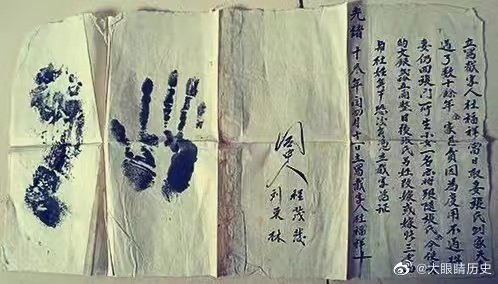
\includegraphics[height=0.36\textwidth,width=0.56\textwidth,viewport=0 0 375 240,clip]{Hand_and_foot-print.png}}

\setlength{\hangindent}{60pt}{\caption*{\hei\hspace{10pt}~ 微博网页提供的清代光绪十八年~(公元1892年)~的休书} }

\setlength{\hangindent}{60pt}{\label{Collect_Liu_Wu}}

\setlength{\hangindent}{60pt}{\end{figure}}

\setlength{\hangindent}{60pt}{\includegraphics{.jpeg}}

\setlength{\hangindent}{60pt}{立写截字人杜福祥}

\setlength{\hangindent}{60pt}{当日娶妻张氏到家,夫妻过了数十余年。余家甚贫,因为度用不过,将妻仍回张门,所生小女一名,亦将跟随张氏。余今休妻的(得)文银贰拾伍两整,日后张氏另姓改嫁,或嫁张三、李四,与杜姓无干。恐说无凭,立截字为证。}

\setlength{\hangindent}{60pt}{\begin{flushright}}

\setlength{\hangindent}{60pt}{光绪十八年~闰四月十一日~立写截字人~~杜福祥 ~~(画 ``十字押'') ~~~\\}

\setlength{\hangindent}{60pt}{\large{同中人~程茂发、刘秉林} ~~~~~~~~~~~~~~~ \\}

\setlength{\hangindent}{60pt}{\huge{手模}、\huge{足印} ~~~~~~~~~~~}

\setlength{\hangindent}{60pt}{\end{flushright}}

\setlength{\hangindent}{60pt}{\newpage}

\setlength{\hangindent}{60pt}{\hypertarget{ux6253ux9c7cux6740ux5bb6-ux4e4b-ux8427ux6069}{%}

\setlength{\hangindent}{60pt}{\subsection{\texorpdfstring{打鱼杀家\protect\footnote{ 此戏是《庆顶珠》中的一部分,据有关资料载,原《庆顶珠》全剧有``得宝''、``庆珠''、``比武''、``珠聘''、``打鱼''、``恶讨''、``屈责''、``献珠''、``杀家''、``投亲''、``劫牢''、``珠圆''等场次。一般习惯从``打鱼''演到``杀家'',故称《打鱼杀家》;旧时戏单``鱼''、``渔''混用,亦作``打渔杀家''。据吴小如先生告,1949年后因田汉建议,戏名统一为《打渔杀家》。{514}}}

\setlength{\hangindent}{60pt}{之}

\setlength{\hangindent}{60pt}{萧恩}{打鱼杀家514 之 萧恩}}\label{ux6253ux9c7cux6740ux5bb6-ux4e4b-ux8427ux6069}}}

\setlength{\hangindent}{60pt}{{{[}第一场{]}}}

\setlength{\hangindent}{60pt}{{开船呐!}}

\setlength{\hangindent}{60pt}{{儿啊------}}

\setlength{\hangindent}{60pt}{{【{\akai 西皮摇板}】父女打鱼在河下,家贫哪怕人笑咱。拉住篷索父把网撒,}}

\setlength{\hangindent}{60pt}{{【{\akai 西皮散板}】年纪衰迈气力不佳。}}

\setlength{\hangindent}{60pt}{{唉,本当不做这河下生意,你我父女何以度日呀?}}

\setlength{\hangindent}{60pt}{{儿啊,不要啼哭,将船湾在柳荫之下,凉爽凉爽。}}

\setlength{\hangindent}{60pt}{{儿啊,将几尾鲜鱼烹煮好了,少时为父还要饮酒。}}

\setlength{\hangindent}{60pt}{{有人唤我。}}

\setlength{\hangindent}{60pt}{{是哪一位?}}

\setlength{\hangindent}{60pt}{{哦,原来是李贤弟。}}

\setlength{\hangindent}{60pt}{{敢莫要到舟中走走?}}

\setlength{\hangindent}{60pt}{{待我搭了扶手。}}

\setlength{\hangindent}{60pt}{{此位是------?}}

\setlength{\hangindent}{60pt}{{(惊介)这做什么?}}

\setlength{\hangindent}{60pt}{{老了,不中用了。}}

\setlength{\hangindent}{60pt}{{儿啊,出舱来见过二位叔父。}}

\setlength{\hangindent}{60pt}{{小女桂英。}}

\setlength{\hangindent}{60pt}{{一十六岁,痴长啊。}}

\setlength{\hangindent}{60pt}{{且慢,方才打得几尾鲜鱼,就在船头之上,你我弟兄畅快饮一回。}}

\setlength{\hangindent}{60pt}{{儿啊,看酒来。}}

\setlength{\hangindent}{60pt}{{啊,二位贤弟,愚兄有个酒令儿。}}

\setlength{\hangindent}{60pt}{愚兄做的是河下生意,忌的是``干''、``旱''二字。}

\setlength{\hangindent}{60pt}{不敢说罚,要敬酒三杯。}

\setlength{\hangindent}{60pt}{请------}

\setlength{\hangindent}{60pt}{呃,敬你三杯。}

\setlength{\hangindent}{60pt}{哦,待我看来。}

\setlength{\hangindent}{60pt}{诶!做什么的?}

\setlength{\hangindent}{60pt}{问的是哪一家呀?}

\setlength{\hangindent}{60pt}{你来看,就在前面,八字粉墙,合脊门楼,那就是丁$\cdots{}\cdots{}$}

\setlength{\hangindent}{60pt}{诶,哼,放肆!}

\setlength{\hangindent}{60pt}{量他也不敢呐。}

\setlength{\hangindent}{60pt}{请------}

\setlength{\hangindent}{60pt}{哦,又有人唤我。}

\setlength{\hangindent}{60pt}{二位贤弟再饮几杯。}

\setlength{\hangindent}{60pt}{哦,原来是丁郎儿,到此何事啊?}

\setlength{\hangindent}{60pt}{你来看,这几日天旱水浅,鱼不上网。改日有了银钱,送上府去。}

\setlength{\hangindent}{60pt}{哦,是是是。}

\setlength{\hangindent}{60pt}{放他去罢,}

\setlength{\hangindent}{60pt}{教他去罢。}

\setlength{\hangindent}{60pt}{(李俊、倪荣\hspace{30pt}~ 啊,萧兄为何这等$\cdots{}\cdots{}$。) }

\setlength{\hangindent}{60pt}{他们的人多。}

\setlength{\hangindent}{60pt}{他们的势力大。}

\setlength{\hangindent}{60pt}{这就难讲话了。}

\setlength{\hangindent}{60pt}{本当不做河下生意,怎奈这囊中------唉,惭愧。}

\setlength{\hangindent}{60pt}{哪位贤弟送来?}

\setlength{\hangindent}{60pt}{当面谢过。}

\setlength{\hangindent}{60pt}{有了人家了。}

\setlength{\hangindent}{60pt}{花荣之子,名唤花逢春。}

\setlength{\hangindent}{60pt}{请------}

\setlength{\hangindent}{60pt}{二位贤弟慢走,愚兄不能远送了。}

\setlength{\hangindent}{60pt}{哦,来了。}

\setlength{\hangindent}{60pt}{儿问的是他?}

\setlength{\hangindent}{60pt}{儿啊------}

\setlength{\hangindent}{60pt}{{【{\akai 西皮摇板}】他本江湖二豪侠,倪荣、李俊就是他。蟒袍、玉带不愿挂,弟兄双双走天涯。}}

\setlength{\hangindent}{60pt}{{【{\akai 西皮散板}】猛抬头见红日坠落西斜。}}

\setlength{\hangindent}{60pt}{{儿啊,天色不早,我们回去了吧。}}

\setlength{\hangindent}{60pt}{{正是: ({\akai 念})父女打鱼在江下,}}

\setlength{\hangindent}{60pt}{{({\akai 念})堪堪不觉红日落,}}

\setlength{\hangindent}{60pt}{{[}第二场{]}}

\setlength{\hangindent}{60pt}{{【{\akai 西皮快三眼}】昨夜晚吃酒醉和衣而卧,稼场鸡惊醒了梦里南柯。二贤弟在河下相劝与我,他教我把打鱼的事啊一旦丢却。我本当不打鱼啊关门闲坐,怎奈我家贫穷无计奈何。清早起开柴扉乌鸦叫过,飞过来叫过去【转西皮二六}】却是为何。将身儿来至在草堂内坐,桂英儿取茶来为父解渴。}}

\setlength{\hangindent}{60pt}{{不教儿渔家打扮,怎么偏偏要渔家打扮?}}

\setlength{\hangindent}{60pt}{{呃------不听父言,就为不孝哇。}}

\setlength{\hangindent}{60pt}{{这便才是!}}

\setlength{\hangindent}{60pt}{{是哪个?}}

\setlength{\hangindent}{60pt}{{你们是哪里来的?}}

\setlength{\hangindent}{60pt}{{哦,原来是丁府上的教师爷。}}

\setlength{\hangindent}{60pt}{{哼!}}

\setlength{\hangindent}{60pt}{{做什么来了?}}

\setlength{\hangindent}{60pt}{{这几日天旱水浅,鱼不上网。改日有钱,送上府去,何必你来!}}

\setlength{\hangindent}{60pt}{{旁人来了无有,教师爷你来了么,}}

\setlength{\hangindent}{60pt}{{哼哼,越发的无有了!}}

\setlength{\hangindent}{60pt}{{朝廷王法,要它何用?}}

\setlength{\hangindent}{60pt}{{哼!}}

\setlength{\hangindent}{60pt}{{哼,尔要锁?}}

\setlength{\hangindent}{60pt}{{当真要锁?}}

\setlength{\hangindent}{60pt}{{果然要锁?}}

\setlength{\hangindent}{60pt}{{如此你就------锁!}}

\setlength{\hangindent}{60pt}{{不教锁。}}

\setlength{\hangindent}{60pt}{{哼!}}

\setlength{\hangindent}{60pt}{{话么,倒是两句好话呀,可惜呀可惜,}}

\setlength{\hangindent}{60pt}{{可惜你二大爷无有工夫啊。}}

\setlength{\hangindent}{60pt}{{尔要讲打?}}

\setlength{\hangindent}{60pt}{{诶呀!老汉幼年间,听说打架,如同小孩子穿新鞋、过新年的一般;如今呐------老了,打不动了啊!}}

\setlength{\hangindent}{60pt}{{尔当真要打?}}

\setlength{\hangindent}{60pt}{{果然要打?!}}

\setlength{\hangindent}{60pt}{{娃娃!待老汉将衣帽留在家中,打个样儿与你们见识见识。}}

\setlength{\hangindent}{60pt}{{【{\akai 西皮导板}】听一言不由我七窍冒火,}}

\setlength{\hangindent}{60pt}{{【{\akai 西皮摇板}】不由我年迈人咬碎牙车}\protect\footnote{ 据樊百乐君告知,刘曾复先生强调,``牙车''是``牙床''的意思。吴小如先生曾撰文指出,天津的王庾生先生此句唱作``这才是闭门坐平地生波''。{515}}{。江湖上叫萧恩不才是我,}}

\setlength{\hangindent}{60pt}{{【{\akai 西皮摇板}】大战场、小战场见过许多。爷本是出山虎独自一个,}}

\setlength{\hangindent}{60pt}{{【{\akai 西皮摇板}】尔好比看家犬一群一窝。你本是奴下奴敢来欺我。}}

\setlength{\hangindent}{60pt}{{慢说是三``羊头'',就是尔这三``狗头'',二大爷何惧!}}

\setlength{\hangindent}{60pt}{{你是丁府上的教师爷?}}

\setlength{\hangindent}{60pt}{{你好本领呐!老汉要领教领教。}}

\setlength{\hangindent}{60pt}{{一定要领教。}}

\setlength{\hangindent}{60pt}{{这是大十八般武艺?}}

\setlength{\hangindent}{60pt}{{这小十八样兵器?}}

\setlength{\hangindent}{60pt}{{这拳脚是?}}

\setlength{\hangindent}{60pt}{{软硬功夫?}}

\setlength{\hangindent}{60pt}{{呃,这叫什么?}}

\setlength{\hangindent}{60pt}{{不好哇。}}

\setlength{\hangindent}{60pt}{{这叫什么?}}

\setlength{\hangindent}{60pt}{{呃,不好。}}

\setlength{\hangindent}{60pt}{{呃,越发的不好啊。}}

\setlength{\hangindent}{60pt}{{方才撞了老汉三``羊头'',如今我要打你三拳头,放你过去。}}

\setlength{\hangindent}{60pt}{{哪里有功夫。}}

\setlength{\hangindent}{60pt}{{着打!}}

\setlength{\hangindent}{60pt}{{着打!}}

\setlength{\hangindent}{60pt}{{打得好,只恐打出祸来了!}}

\setlength{\hangindent}{60pt}{{那贼回去,定不甘休。待为父赶至县衙,抢他一个原告!}}

\setlength{\hangindent}{60pt}{{不要儿管,取为父的衣帽过来。}}

\setlength{\hangindent}{60pt}{{好好看守门户,为父去去就来。}\protect\footnote{ 陈超老师注: 刘曾复先生曾说明: 此处萧恩\textless{}\!{\bfseries\akai 扫头}\!\textgreater{}下场,不踢大带: 出门,褶子倒手,右手向上一指,弹髯下。这个\textless{}\!{\bfseries\akai 扫头}\!\textgreater{}扫的是一个``对儿'',``闭门家中坐,祸从天上来'',因此这一指表示``祸从天上来''。{516}}}

\setlength{\hangindent}{60pt}{{[}第三场{]}}

\setlength{\hangindent}{60pt}{{(萧桂英}

\setlength{\hangindent}{60pt}{【{\akai 西皮散板}】老爹爹清晨出前去出首,)}\protect\footnote{ 刘曾复先生为樊百乐君说《审刺客》一戏时,顺便说了``萧恩挨打''部分的内容。{517}}}

\setlength{\hangindent}{60pt}{{(众\hspace{40pt}~ ({\akai 内})一十!)} }

\setlength{\hangindent}{60pt}{{(萧桂英\hspace{40pt}~ 【{\akai 西皮散板}】倒叫我桂英儿挂在心头。)} }

\setlength{\hangindent}{60pt}{{(众\hspace{40pt}~ ({\akai 内})二十!)} }

\setlength{\hangindent}{60pt}{{(萧桂英\hspace{40pt}~ 【{\akai 西皮散板}】将身儿来至在草堂门口,)} }

\setlength{\hangindent}{60pt}{{(众\hspace{40pt}~ ({\akai 内})三十!)} }

\setlength{\hangindent}{60pt}{{(萧桂英\hspace{40pt}~ 【{\akai 西皮散板}】只等得爹爹回细问根由。)} }

\setlength{\hangindent}{60pt}{{(众\hspace{40pt}~ ({\akai 内})四十打完!)} }

\setlength{\hangindent}{60pt}{{(吕子秋\hspace{40pt}~ ({\akai 内})赶下堂去!)} }

\setlength{\hangindent}{60pt}{{好贼!}}

\setlength{\hangindent}{60pt}{{【{\akai 西皮散板}】恼恨那吕子秋为官不正,仗势力欺压我受苦的良民呐。上堂来他那里一言不问,责打我四十板呐赶出了头门。}}

\setlength{\hangindent}{60pt}{{【{\akai 西皮散板}】我这里咬牙关忙往家奔,叫一声桂英儿你快来开门呐。}}

\setlength{\hangindent}{60pt}{{为父上得堂去,那贼一言不问,将为父重责。}}

\setlength{\hangindent}{60pt}{{这还不算受屈。他教为父连夜过江与那老贼赔礼,那才算受屈呢。}}

\setlength{\hangindent}{60pt}{{哎呀------我恨不得飞过江去,我就杀$\cdots{}\cdots{}$}}

\setlength{\hangindent}{60pt}{{我要杀贼的满门,方消我心头之恨!}}

\setlength{\hangindent}{60pt}{{小小年纪,懂得什么?!不用多管,取为父衣帽、戒刀过来。}}

\setlength{\hangindent}{60pt}{{不用儿管,快些取来。}}

\setlength{\hangindent}{60pt}{{为父去也。}}

\setlength{\hangindent}{60pt}{{何事?}}

\setlength{\hangindent}{60pt}{{小小年纪,去之无益。}}

\setlength{\hangindent}{60pt}{{有此胆量?}}

\setlength{\hangindent}{60pt}{{快将儿的衣服、兵刃收拾好了。}}

\setlength{\hangindent}{60pt}{{壮胆量也是好的。}}

\setlength{\hangindent}{60pt}{{走哇$\cdots{}\cdots{}$}}

\setlength{\hangindent}{60pt}{{做什么?}}

\setlength{\hangindent}{60pt}{{这门么,关也罢,不关也罢呀。}}

\setlength{\hangindent}{60pt}{{又做什么?}}

\setlength{\hangindent}{60pt}{{唉!门都不要了,还要什么家具呀?}}

\setlength{\hangindent}{60pt}{{唉,不明白的冤家呀,呃$\cdots{}\cdots{}$(哭介)}}

\setlength{\hangindent}{60pt}{{不要啼哭,随为父的走哇。}}

\setlength{\hangindent}{60pt}{{儿啊,此番前去,教儿骂,儿就骂,教儿杀,儿就杀,不要害怕。}}

\setlength{\hangindent}{60pt}{{走哇。}}

\setlength{\hangindent}{60pt}{{儿啊,夜晚行船,比不得白日,儿要掌稳了舵!}}

\setlength{\hangindent}{60pt}{{【{\akai 西皮快板}】这件事不由我心头冒火,今夜晚过江去将他杀却。恨不得插双翅江河越过,}}

\setlength{\hangindent}{60pt}{{【{\akai 西皮散板}】我的儿因何故放了篷索。}}

\setlength{\hangindent}{60pt}{{杀人还有什么假的不成?}}

\setlength{\hangindent}{60pt}{{呀呸!为父在家中不教儿前来,儿是偏偏地要来。这船行半江之中,儿又要回去------也罢!待为父拨转船头,送儿回去。}}

\setlength{\hangindent}{60pt}{{\textless{}哭头\textgreater{}啊,桂英,我的儿呀!}}

\setlength{\hangindent}{60pt}{{少时还在此处上船,儿记下了?}}

\setlength{\hangindent}{60pt}{{儿啊,庆顶珠}\protect\footnote{ 吴小如先生告,萧恩对萧桂英提及``庆顶珠''时,念白作``聘礼珠子'',``庆顶珠''作戏名。{518}}{可在身旁?}}

\setlength{\hangindent}{60pt}{{此番前去,倘有不测,儿自带庆顶珠逃往花家去吧。}}

\setlength{\hangindent}{60pt}{{我么------儿就不用管了哇。}}

\setlength{\hangindent}{60pt}{{不要啼哭,随我走哇。}}

\setlength{\hangindent}{60pt}{{来此已是。}}

\setlength{\hangindent}{60pt}{{且慢。}}

\setlength{\hangindent}{60pt}{{收拾好了。}}

\setlength{\hangindent}{60pt}{{有人么?走出一个来呀。}}

\setlength{\hangindent}{60pt}{{过府赔罪来了。}}

\setlength{\hangindent}{60pt}{{哼!}}

\setlength{\hangindent}{60pt}{{请了。}}

\setlength{\hangindent}{60pt}{{我来问你: 这鱼税银子,可有圣上旨意?}}

\setlength{\hangindent}{60pt}{{户部公文?}}

\setlength{\hangindent}{60pt}{{凭着何来?}}

\setlength{\hangindent}{60pt}{{敢是那吕子秋?!}}

\setlength{\hangindent}{60pt}{{哼!}}

\setlength{\hangindent}{60pt}{{【{\akai 西皮摇板}】这税银我不纳是我的本分,你不该差人役打上我门。}}

\setlength{\hangindent}{60pt}{{儿啊,骂呀!}}

\setlength{\hangindent}{60pt}{{且慢,我父女有好心献上。}}

\setlength{\hangindent}{60pt}{{打鱼之时,得来一宗宝贝,名唤庆顶珠。}}

\setlength{\hangindent}{60pt}{{这$\cdots{}\cdots{}$耳目甚多。}}

\setlength{\hangindent}{60pt}{{看刀!}}

\setlength{\hangindent}{60pt}{{儿啊,随为父的杀呀!}}

\setlength{\hangindent}{60pt}{\newpage}

\setlength{\hangindent}{60pt}{\hypertarget{ux7843ux7802ux75e3-ux4e4b-ux97e9ux5ef7ux51e4ux8c2dux6d3e}{%}

\setlength{\hangindent}{60pt}{\subsection{硃砂痣 之}

\setlength{\hangindent}{60pt}{韩廷凤(谭派)}\label{ux7843ux7802ux75e3-ux4e4b-ux97e9ux5ef7ux51e4ux8c2dux6d3e}}}

\setlength{\hangindent}{60pt}{{{[}第一场{]}}}

\setlength{\hangindent}{60pt}{{唉!}}

\setlength{\hangindent}{60pt}{{【{\akai 二黄摇板}】为续弦前后厅灯光明亮,梦不想今夜晚再做新郎。}}

\setlength{\hangindent}{60pt}{{抬上堂来({\akai 或}: }搭上堂来)\protect\footnote{ 以下括号中的念白据吴焕老师整理的剧本(经刘曾复先生审订)添加。{519}}{。}}

\setlength{\hangindent}{60pt}{{每人赏银二分({\akai 或}: }每人赏钱四个){。}}

\setlength{\hangindent}{60pt}{{带他们下面用饭。}}

\setlength{\hangindent}{60pt}{{待我观看一回。}}

\setlength{\hangindent}{60pt}{{【{\akai 二黄慢板}】我这里借灯光用目观望,我看她({\akai 或}: 只见她)与前妻一样风光。}}

\setlength{\hangindent}{60pt}{{【{\akai 二黄慢板}】为什么({\akai 或}: 因何故)皱眉间泪带面上({\akai 或}: 泪带脸上),莫不是嫌年迈难配鸾凰。}}

\setlength{\hangindent}{60pt}{{【{\akai 二黄慢板}】要穿衣锦绣衫任你选样,}}

\setlength{\hangindent}{60pt}{{【{\akai 二黄慢板}】要用饭现有那谷米陈仓。}}

\setlength{\hangindent}{60pt}{{【{\akai 二黄慢板}】这不是那不是难以猜想,尊娘行({\akai 或}: 问娘行)因何事珠泪汪汪,为的是哪桩,你何妨({\akai 或}: 又何妨)细说端详?}}

\setlength{\hangindent}{60pt}{{【{\akai 二黄摇板}】听她言这婚姻({\akai 或}: 好一似)冰结霜降,一时里惹动我烦恼愁肠。看起来断不可此事勾当,自情愿伴孤灯独守空房。}}

\setlength{\hangindent}{60pt}{{韩福过来。}}

\setlength{\hangindent}{60pt}{{命你同媒婆送这位大娘子回去,对他丈夫言讲({\akai 或}: 与他丈夫言讲): 前番(那)一百两银子不要,再送他一百两银子,教他好好将养疾病,将大娘子送回,成全他夫妻恩义。就此去罢。}}

\setlength{\hangindent}{60pt}{{啊大娘子,还有这婚书呢。}}

\setlength{\hangindent}{60pt}{{唉,就在灯前焚化了罢。}}

\setlength{\hangindent}{60pt}{{【{\akai 二黄摇板}】伊言道她丈夫病卧床上,没奈何卖妻子暂度时光。将自己比旁人俱是({\akai 或}: 皆是)一样,我岂肯拆散他恩爱鸳鸯。({\akai 或}: 善与恶自有那天理昭彰。)}}

\setlength{\hangindent}{60pt}{{{[}第二场{]}}}

\setlength{\hangindent}{60pt}{{【{\akai 二黄摇板}\protect\footnote{ 据吴焕老师整理的剧本注: 汪派在``想当年''前面还有两句,词句是``劝世人一个个须要学好,皆因是自有那天理昭彰。''{520}}{】想当年为太守何等荣耀,遇兵荒妻和子无有下梢。多亏了陈太尉将我来保,才能得归田园自在逍遥。}}

\setlength{\hangindent}{60pt}{{【{\akai 二黄摇板}】忙迫中呃挽定了把礼还到,一时里好教我难解根苗。}}

\setlength{\hangindent}{60pt}{{呜,你不是昨晚送回去的大娘子么?}}

\setlength{\hangindent}{60pt}{{既然将你送回,你又来则甚呐?}}

\setlength{\hangindent}{60pt}{{哦,(原来是)吴相公来了。}}

\setlength{\hangindent}{60pt}{{哎呀,请坐请坐。}}

\setlength{\hangindent}{60pt}{{呃,还有话讲啊。}}

\setlength{\hangindent}{60pt}{{(有话叙谈,}哪有不坐之理,请坐请坐。{)}}

\setlength{\hangindent}{60pt}{{啊大娘子,你也坐下。}}

\setlength{\hangindent}{60pt}{{啊吴相公,昨日听得大娘子说到家中一番苦楚,甚是凄惨。相公有恙在身,改日再来叙谈,为何带病前来?({\akai 或}: 大相公,昨日听得大娘子说到家中一番苦楚。相公你有病在床,病体好了,再来不迟。)}}

\setlength{\hangindent}{60pt}{{哦,你见了银子,出了一身的通汗,这病就好了么?}}

\setlength{\hangindent}{60pt}{{哎呀呀,吴相公啊,看将起来,这银子啊,是好物件!}}

\setlength{\hangindent}{60pt}{{【{\akai 二黄碰板垛板}】我救你的急,救你的难,救你的贫困;全尔的节,全尔的义,全尔的婚呐姻。纵有妻不生子前生造定,我岂肯拆婚姻}\protect\footnote{ 此处刘曾复先生说戏录音近似``错婚姻'',吴小如先生从夏山楼主学的是``拆婚姻'',此处从吴小如先生。李楠君认为,此处系刘曾复先生将``拆''字按上口字处理。{521}}{落下了骂名。}}

\setlength{\hangindent}{60pt}{{啊,啊,呵呵呵哈哈哈$\cdots{}\cdots{}$(笑介)}}

\setlength{\hangindent}{60pt}{{请坐请坐。}}

\setlength{\hangindent}{60pt}{{哎呀呀吴相公啊,我当日也是恩爱夫妻,只因兵荒马乱,中途失散,却无子嗣。若有一子传宗接代,我也就不续弦再娶的了哇。}}

\setlength{\hangindent}{60pt}{{这$\cdots{}\cdots{}$子孙前世所修,再续么,也就不必了。({\akai 或}: }子孙之事,前生所修。再娶么,唉,也就不必了。{)}}

\setlength{\hangindent}{60pt}{{言得极是,只是本处孩儿多有不便呐。}}

\setlength{\hangindent}{60pt}{{本当如此,奈无机会。}}

\setlength{\hangindent}{60pt}{{这只好凭天机、遇时宜了。}}

\setlength{\hangindent}{60pt}{{吴相公慢些走啊!}}

\setlength{\hangindent}{60pt}{{【{\akai 二黄摇板}】他夫妻进门来双双拜倒({\akai 或}: 双双跪倒),口声声叫恩人泪似呃雨抛。非是我用银钱假意行好哇,韩廷凤全仁义一片心苗。}}

\setlength{\hangindent}{60pt}{{{[}第三场{]}}}

\setlength{\hangindent}{60pt}{{【四平调】叹光阴去不归无限烦闷,不觉已老两鬓如银。读古书难解我心头烦闷,饮香醪怎畅我衷肠凄清。}}

\setlength{\hangindent}{60pt}{{哦,你是吴相公,呃,请坐请坐。}}

\setlength{\hangindent}{60pt}{{你往成都收取账目,呃,必定是发了财了哇。({\akai 或}: }闻你往成都,收取账目,一定发财的了。{)}}

\setlength{\hangindent}{60pt}{{请便。}}

\setlength{\hangindent}{60pt}{{哦,这是何人?}}

\setlength{\hangindent}{60pt}{{哦,罢了(罢了),一旁坐下。}}

\setlength{\hangindent}{60pt}{{呃,不妨不妨,只管地坐下。}}

\setlength{\hangindent}{60pt}{{呵呵呵哈哈哈$\cdots{}\cdots{}$(笑介)}}

\setlength{\hangindent}{60pt}{{啊吴相公,你看这小小的孩童,呃,也(很)知大体呀。}}

\setlength{\hangindent}{60pt}{{是啊,小孩子原要(他)爹娘教导哇。}}

\setlength{\hangindent}{60pt}{{啊吴相公,你买他前来,还是为子啊,还是为仆呢?}}

\setlength{\hangindent}{60pt}{{哦,这等说来({\akai 或}: }如此说来){,是送与我的?}}

\setlength{\hangindent}{60pt}{{哎呀呀吴相公啊,你真是({\akai 或}: }你真乃){信实人也。}}

\setlength{\hangindent}{60pt}{{【四平调】吴官人你真真言而有信,你与我谋后代不惜辛勤。感谢你这好意情深义尽,\textless{}行弦\textgreater{}}}

\setlength{\hangindent}{60pt}{{吴大哥,你请来上坐。({\akai 或}: }这边坐,这边坐。{)}}

\setlength{\hangindent}{60pt}{{请坐,请坐。}}

\setlength{\hangindent}{60pt}{{【四平调】退一日自当另有条陈。}}

\setlength{\hangindent}{60pt}{{呵呵哈哈哈$\cdots{}\cdots{}$(笑介)}}

\setlength{\hangindent}{60pt}{{哎呀吴官人呐,我如今有了儿子就不愁了。}}

\setlength{\hangindent}{60pt}{{是啊,吴官人离家日久,我也不便相留({\akai 或}: }不便强留{),改日我父子要登门叩谢。}}

\setlength{\hangindent}{60pt}{{儿啊,送过你吴大爷。}}

\setlength{\hangindent}{60pt}{{(啊,吴官人何事?)}}

\setlength{\hangindent}{60pt}{{请来吃酒,请来吃酒。}}

\setlength{\hangindent}{60pt}{{啊$\cdots{}\cdots{}$呃,吴官人,请转请转。}}

\setlength{\hangindent}{60pt}{{改日我父子,呃,要登门再谢。}}

\setlength{\hangindent}{60pt}{{呃一定要去,一定要去。}}

\setlength{\hangindent}{60pt}{{啊$\cdots{}\cdots{}$呃,无有了,请便请便。({\akai 或}: }吴官人,请呐请呐。{)}}

\setlength{\hangindent}{60pt}{{哦------哈哈哈$\cdots{}\cdots{}$(笑介)}}

\setlength{\hangindent}{60pt}{{儿啊,随为父的进来。}}

\setlength{\hangindent}{60pt}{{一旁坐下,待我细看一回({\akai 或}: 待我}细观一回{)。}}

\setlength{\hangindent}{60pt}{{【{\akai 二黄原板}】我的儿须从容端然坐定,看形象并非是平等之人。细观他各部位五官端正,这两鬓齐开朗目秀眉清。儿在家可读过圣贤书本,一一地对为父细说分明。}}

\setlength{\hangindent}{60pt}{{【{\akai 二黄原板}】他说话有分寸智慧聪明,倒像个宦门后不差毫分。可记得是何年月日生辰,说出来将八字细与儿评。}}

\setlength{\hangindent}{60pt}{{【{\akai 二黄原板}】这小娃言语中隐藏暗景,再问他亲父母便知真情。儿父母年多少在不在,因何故图银钱卖与他人。}}

\setlength{\hangindent}{60pt}{{儿今年多大年纪了({\akai 或}: }儿今年几岁了{) ?}}

\setlength{\hangindent}{60pt}{{儿父?}}

\setlength{\hangindent}{60pt}{{死了五载。}}

\setlength{\hangindent}{60pt}{{儿母?}}

\setlength{\hangindent}{60pt}{{七旬有余。}}

\setlength{\hangindent}{60pt}{{(惊介)儿有一十三岁({\akai 或}: }儿才一十三岁{)。}}

\setlength{\hangindent}{60pt}{{(惊介)嗯$\cdots{}\cdots{}$}}

\setlength{\hangindent}{60pt}{{【{\akai 二黄原板}】这其间又盘出}\protect\footnote{ 吴焕老师整理的剧本记作``又攀出''。{522}}{奇情种种,哪有个花甲年又产娇生。}}

\setlength{\hangindent}{60pt}{{儿啊------}}

\setlength{\hangindent}{60pt}{{【{\akai 二黄原板}】必然是那老娘将儿蒙混,这内中另有个生儿的娘亲。}}

\setlength{\hangindent}{60pt}{{哦,儿是捡来的么?}}

\setlength{\hangindent}{60pt}{{【{\akai 二黄原板}】细盘问这来由日月推论,仔细想当年事越加是真: 宣和年四月里成都调任,行至在青州府路遇贼兵。亲生儿在娘怀无有踪影,实可怜贤德妻命赴幽冥。}}

\setlength{\hangindent}{60pt}{{【{\akai 二黄散板}】这形象好一似韩门真种,举动间与老夫骨肉有情。我这里取菱花照照相品呐,}}

\setlength{\hangindent}{60pt}{{【{\akai 二黄散板}】半像我半像妻不差毫分。}}

\setlength{\hangindent}{60pt}{{【{\akai 二黄散板}】亲生子再相逢三生有幸,这才是天地意弄假成真。}}

\setlength{\hangindent}{60pt}{{不对了,不对了!}}

\setlength{\hangindent}{60pt}{{(韩玉印\hspace{40pt}~ 怎么不对呢?)} }

\setlength{\hangindent}{60pt}{{我那亲生的孩儿,落生下来,左足心上有硃砂红痣。你无有,不是我的亲生儿子啊。}}

\setlength{\hangindent}{60pt}{{怎么,儿也有?}}

\setlength{\hangindent}{60pt}{{为父的不信呐,待我看来。}}

\setlength{\hangindent}{60pt}{{(唉,儿啊------)}}

\setlength{\hangindent}{60pt}{{【{\akai 二黄散板}】你是我亲生的儿呀名唤玉印,遇兵荒遭失散十有二春。盼娇儿盼得我身染重病,盼娇儿盼得我昼夜不宁。盼娇儿啊不做官告归故呃井,喂呀我的儿呀,梦不想天保佑枯木哇逢春。}}

\setlength{\hangindent}{60pt}{{你母命丧东平,也曾命人搬尸去了$\cdots{}\cdots{}$哇,呃$\cdots{}\cdots{}$(哭介)}}

\setlength{\hangindent}{60pt}{{言得极是,派人接她前来就是。}}

\setlength{\hangindent}{60pt}{{正是: ({\akai 念})北转南来西复东,今朝骨肉又重逢。父子再把菱花照,}}

\setlength{\hangindent}{60pt}{{(儿啊------)}}

\setlength{\hangindent}{60pt}{{({\akai 念})只怕相逢在梦中。}}

\setlength{\hangindent}{60pt}{{哦,不是做梦?}}

\setlength{\hangindent}{60pt}{{玉印,我儿,啊------啊------哈哈哈$\cdots{}\cdots{}$(笑介)}}

\setlength{\hangindent}{60pt}{{随我来。}}

\setlength{\hangindent}{60pt}{\newpage}

\setlength{\hangindent}{60pt}{\hypertarget{ux96c4ux5ddeux5173}{%}

\setlength{\hangindent}{60pt}{\subsection{雄州关}\label{ux96c4ux5ddeux5173}}}

\setlength{\hangindent}{60pt}{{{[}第一场{]}}}

\setlength{\hangindent}{60pt}{{呼延狄\hspace{40pt}~ ({\akai 念})百万熊罴犯中原,} }

\setlength{\hangindent}{60pt}{{雷洪切\hspace{40pt}~ ({\akai 念})搅乱宋室不安然!} }

\setlength{\hangindent}{60pt}{{达林呈\hspace{40pt}~ ({\akai 念})渴饮马上刀头血,} }

\setlength{\hangindent}{60pt}{{季乐芬\hspace{40pt}~ ({\akai 念})嘿!饥饿人头当饭餐!} }

\setlength{\hangindent}{60pt}{{众\hspace{40pt}~ 俺------} }

\setlength{\hangindent}{60pt}{{呼延狄\hspace{40pt}~ 金邦大将军呼延狄是也!} }

\setlength{\hangindent}{60pt}{{雷洪切\hspace{40pt}~ 金邦副将军雷洪切是也!} }

\setlength{\hangindent}{60pt}{{达林呈\hspace{40pt}~ 金邦左先锋达林呈是也!} }

\setlength{\hangindent}{60pt}{{季乐芬\hspace{40pt}~ 金邦右先锋季乐芬是也!} }

\setlength{\hangindent}{60pt}{{萨里哈\hspace{40pt}~ 前营骁骑大将军萨里哈是也!} }

\setlength{\hangindent}{60pt}{{耶律浑\hspace{40pt}~ 后营骁骑大将军耶律浑是也!} }

\setlength{\hangindent}{60pt}{{提尔雄\hspace{40pt}~ 左营压队大将军提尔雄是也!} }

\setlength{\hangindent}{60pt}{{虎骨达\hspace{40pt}~ 右营护卫大将军虎骨达是也!} }

\setlength{\hangindent}{60pt}{{呼延狄\hspace{40pt}~ 列位将军请了------} }

\setlength{\hangindent}{60pt}{{众\hspace{40pt}~ 请了!} }

\setlength{\hangindent}{60pt}{{呼延狄}

\setlength{\hangindent}{60pt}{你我奉了狼主之命,随定四太子,领兵夺取宋室天下,兵到即克。也是宋王气数当尽了。}}

\setlength{\hangindent}{60pt}{{众\hspace{40pt}~ 着啊!} }

\setlength{\hangindent}{60pt}{{呼延狄\hspace{40pt}~ 这些蛮子怎能苦争恶战,这也是我家狼主洪福齐天也!} }

\setlength{\hangindent}{60pt}{{众}

\setlength{\hangindent}{60pt}{听觱篥}\protect\footnote{ 段公平君注: 觱篥,又作``筚篥'',竹管乐器,源于西域,类似``胡笳''。即俗称``牛角觱篥''者,番邦号角。{523}}{一声响,太子升帐,你我两厢伺候。请------}}

\setlength{\hangindent}{60pt}{{金兀朮}

\setlength{\hangindent}{60pt}{\textless{}点绛唇\textgreater{}军营号响}\protect\footnote{ 段公平君建议作``各路豪强''。{524}}{,威武雄壮;中军帐,排列刀枪,杀气呃------}}

\setlength{\hangindent}{60pt}{{众\hspace{40pt}~ 参见殿下!} }

\setlength{\hangindent}{60pt}{{金兀朮\hspace{40pt}~ 站立两厢!} }

\setlength{\hangindent}{60pt}{{金兀朮}

\setlength{\hangindent}{60pt}{({\akai 念})杀气腾腾满乾坤,哀声处处震天庭。宋王失政宠奸佞,锦绣江山一旦倾。}}

\setlength{\hangindent}{60pt}{{金兀朮}

\setlength{\hangindent}{60pt}{孤,北番大金邦女真国老王殿下四太子、昌平王、御营总兵完颜兀朮。今有宋主无道,宠信奸臣。内奸童贯封为广阳王}\protect\footnote{ 此处从《传统剧目汇编》,童贯封``广阳王''。{525}}{之职。是他前者有密书到孤父王驾下,约定我国兴兵夺取他家社稷。有他以为内应,这宋室天下岂不是唾手而得。自兴兵以来,战无不胜,攻无不取。前日又破了潞安州,守将陆登自刎身亡,甚是悲惨。前面乃是雄州关,守将韩世忠。此人乃是忠勇之士,孤家不忍逼迫于他。意欲招他归顺,助孤一臂之力,何愁大事不成。}}

\setlength{\hangindent}{60pt}{{金兀朮\hspace{40pt}~ 众番儿!} }

\setlength{\hangindent}{60pt}{{众\hspace{40pt}~ 有!} }

\setlength{\hangindent}{60pt}{{金兀朮\hspace{40pt}~ 此番兴兵行至雄州关,不可杀掠黎民,违令者斩!} }

\setlength{\hangindent}{60pt}{{众\hspace{40pt}~ 啊!} }

\setlength{\hangindent}{60pt}{{金兀朮\hspace{40pt}~ 由此发动人马!} }

\setlength{\hangindent}{60pt}{{{[}第二场{]}}}

\setlength{\hangindent}{60pt}{{探子\hspace{40pt}~ 马来。} }

\setlength{\hangindent}{60pt}{{探子}

\setlength{\hangindent}{60pt}{({\akai 念})短甲随身衲袄齐,肩上横担令字旗。年年岁岁领皇赏。一马冲至军队里。}}

\setlength{\hangindent}{60pt}{{探子}

\setlength{\hangindent}{60pt}{俺,韩元帅麾下能行探子是也。奉了元帅将令,着俺四路哨探。今有圣上差孙浩督兵前来剿灭金邦,已至三山口。不免飞骑报韩元帅知道!就此马上加鞭。}}

\setlength{\hangindent}{60pt}{{{[}第三场{]}}}

\setlength{\hangindent}{60pt}{{韩世忠}

\setlength{\hangindent}{60pt}{【{\akai 西皮三眼}】为金兵急得我心神不定,盼救}兵望眼穿昼夜不宁。陆元帅尽了忠自刎丧命,只一子失陷在万马军营。好教人止不住啊【转{西皮二六}】腮边泪滚,可叹他夫妻们饮恨幽冥。行公文\protect\footnote{ 夏行涛君建议作``赍公文''。{526}}求圣上遣将助阵,因何故十数日渺无回音。在二堂思无计心呃中忧闷,我父子只恐怕难退雄兵。}

\setlength{\hangindent}{60pt}{中军\hspace{40pt}~ ({\akai 念})探马如飞急,叩禀元帅知。 }

\setlength{\hangindent}{60pt}{中军\hspace{40pt}~ 启元帅: 探马求见。 }

\setlength{\hangindent}{60pt}{韩世忠\hspace{40pt}~ 吩咐开门! }

\setlength{\hangindent}{60pt}{中军\hspace{40pt}~ 开门! }

\setlength{\hangindent}{60pt}{众\hspace{40pt}~ 啊! }

\setlength{\hangindent}{60pt}{韩世忠\hspace{40pt}~ {({\akai 念})}探马报音信,升帐问分明。 }

\setlength{\hangindent}{60pt}{韩世忠\hspace{40pt}~ 传探马。 }

\setlength{\hangindent}{60pt}{中军\hspace{40pt}~ 元帅有令: 探马进见。 }

\setlength{\hangindent}{60pt}{探马\hspace{40pt}~ 报------告进。 }

\setlength{\hangindent}{60pt}{探马\hspace{40pt}~ 帅爷在上,探马叩头。 }

\setlength{\hangindent}{60pt}{韩世忠\hspace{40pt}~ 打听哪路军情,起来快些讲。 }

\setlength{\hangindent}{60pt}{探马\hspace{40pt}~ 啊,帅爷听禀:  }

\setlength{\hangindent}{60pt}{探马}

\setlength{\hangindent}{60pt}{({\akai 念})一马哨探似流星,朝中差来孙总兵。十万人马到疆界,禀报元帅得知情。}

\setlength{\hangindent}{60pt}{韩世忠\hspace{40pt}~ 朝中无有什么姓孙的呀! }

\setlength{\hangindent}{60pt}{探马\hspace{40pt}~ 在元帅帐下当过副将的。 }

\setlength{\hangindent}{60pt}{韩世忠\hspace{40pt}~ 哦------敢是孙浩?! }

\setlength{\hangindent}{60pt}{探马\hspace{40pt}~ 正是。 }

\setlength{\hangindent}{60pt}{韩世忠\hspace{40pt}~ 赏尔金牌一面,再去打探。 }

\setlength{\hangindent}{60pt}{探马\hspace{40pt}~ 得令! }

\setlength{\hangindent}{60pt}{韩世忠}

\setlength{\hangindent}{60pt}{且住!想那孙浩,在某帐下曾为副将。只因犯我将令,将他捆打,是他逃至京中,投在{广阳}府内,做了随侍。今番奉旨督兵前来,焉有不接之理。}

\setlength{\hangindent}{60pt}{韩世忠\hspace{40pt}~ 中军! }

\setlength{\hangindent}{60pt}{中军\hspace{40pt}~ 有! }

\setlength{\hangindent}{60pt}{韩世忠\hspace{40pt}~ 传众将进帐。 }

\setlength{\hangindent}{60pt}{中军\hspace{40pt}~ 众将进帐呃! }

\setlength{\hangindent}{60pt}{{四将}\hspace{40pt}~ ({\akai 内})来也! }

\setlength{\hangindent}{60pt}{{四将}}

\setlength{\hangindent}{60pt}{({\akai 念})元帅传军令,将士共趋迎\protect\footnote{ 夏行涛君建议作``躬躯迎''。{527}}。}

\setlength{\hangindent}{60pt}{{四将}\hspace{40pt}~ 参见元帅。 }

\setlength{\hangindent}{60pt}{韩世忠\hspace{40pt}~ 众位将军少礼! }

\setlength{\hangindent}{60pt}{{四将}\hspace{40pt}~ 啊! }

\setlength{\hangindent}{60pt}{{四将}\hspace{40pt}~ 传末将等进帐,有何军情议论? }

\setlength{\hangindent}{60pt}{韩世忠\hspace{40pt}~ 圣上命孙浩督兵前来,征剿金人,已到三山口。命你等前去迎接。 }

\setlength{\hangindent}{60pt}{{四将}\hspace{40pt}~ 啊元帅,那孙浩若问: 你家元帅为何不来。我等怎样回答? }

\setlength{\hangindent}{60pt}{韩世忠}

\setlength{\hangindent}{60pt}{你等就说: 我家元帅因金兵犯境,城内空虚,不敢擅离汛地,故命我等前来迎接。}

\setlength{\hangindent}{60pt}{{四将}\hspace{40pt}~ 那孙浩缘何授得此职? }

\setlength{\hangindent}{60pt}{韩世忠\hspace{40pt}~ 唉!你等不知他的来历,听我令下:  }

\setlength{\hangindent}{60pt}{{韩世忠}

\setlength{\hangindent}{60pt}{【{\akai 西皮}原板}】韩世忠坐宝帐传言发令,叫一声众将官细听详情: 那孙浩平日间行为不正,犯军令责罚他不能徇情呃。逃到了京师地{广阳}府进,童太尉听谗言懵懂圣君。迎接他务须要言语谨慎,}

\setlength{\hangindent}{60pt}{{韩世忠\hspace{40pt}~ 【{\akai 西皮摇板}】防贼子寻仇起暗箭伤人。 }

\setlength{\hangindent}{60pt}{{四将\hspace{40pt}~ 得令!} }

\setlength{\hangindent}{60pt}{{四将\hspace{40pt}~ 【{\akai 西皮摇板}】韩元帅忠义士谁人不敬,何惧那孙浩贼势利小人。} }

\setlength{\hangindent}{60pt}{{韩世忠}

\setlength{\hangindent}{60pt}{【{\akai 西皮摇板}】大宋朝八代君徽宗失政,贪酒色戮忠良信宠谗臣。恨蔡京与童贯伤害民命,惹得那四路里齐动刀兵。金兀朮领人马抢夺州郡,逼元戎劳将士苦及黎民。众将官退宝帐各归管汛,}}

\setlength{\hangindent}{60pt}{{韩世忠\hspace{40pt}~ 【{\akai 西皮摇板}】且等候四将回再定计行。} }

\setlength{\hangindent}{60pt}{{{[}第四场{]}}}

\setlength{\hangindent}{60pt}{{孙浩}

\setlength{\hangindent}{60pt}{\textless{}点绛唇\textgreater{}奉旨领雄兵,蟒罗袍,不愧先人;定斩世忠消吾恨,还报他痛打军刑。}}

\setlength{\hangindent}{60pt}{{孙浩}}

\setlength{\hangindent}{60pt}{({\akai 念}){胸怀巧诈极聪明,不近贵人怎升腾?只道一生空劳力,运至时来命通亨。}}

\setlength{\hangindent}{60pt}{{孙浩}

\setlength{\hangindent}{60pt}{某,孙浩,塞北人也。昔在韩世忠麾下以为步军,只因不守军规,专意花酒情浓。抢得一有夫之妇作乐,不想韩世忠便要将俺斩首。是俺推在步兵列名身上,彼时将那步兵斩首号令。又道俺带领无方,将俺捆打,削去头领,赶出不用。俺又羞又恼,一怒奔至京中。恰遇童太尉朝罢而归,是俺闯了他的禁道,将我拿到府中拷问。俺将韩世忠打革之事从头诉说一遍,不想童太尉与韩世忠是旧有仇恨,听了此言,便把俺留在府呃中。因俺善于奉承,是他心中欢喜,想要重用于俺。如今金兀朮兴兵犯界,破了无数城池。眼看要到雄州,那韩世忠本章进京,求兵添将。童太尉奏上一本,命俺提兵前来,剿灭番贼。若是得胜,道韩世忠贪生怕死;若是损兵,便道韩世忠按兵不动。慢说是一个韩世忠,就是百个,也教他有死无生。看前面已是三山口,众将,催动人马!}}

\setlength{\hangindent}{60pt}{{孙浩\hspace{40pt}~ 【{\akai 西皮导板}】见旌旗空中飘人声喧震,} }

\setlength{\hangindent}{60pt}{{孙浩}

\setlength{\hangindent}{60pt}{【{\akai 西皮原板}】抖起}了万丈尘沸沸腾腾。曾记得到京都那般光景,岂料我今日里督领雄兵。韩世忠好比那儿童之分,怎知晓暗中刀要你残生。咱料他如南柯梦魂未醒,}

\setlength{\hangindent}{60pt}{{孙浩\hspace{40pt}~ 【{\akai 西皮摇板}】绑云阳一命倾才晓前情。 }

\setlength{\hangindent}{60pt}{{孙浩}

\setlength{\hangindent}{60pt}{前道}\protect\footnote{ 段公平君建议作``前导''。{528}}{为何不行?}}

\setlength{\hangindent}{60pt}{{四将\hspace{40pt}~ 雄州关总戎麾下四营将校迎接总爷。} }

\setlength{\hangindent}{60pt}{{众\hspace{40pt}~ 雄州关总戎麾下四营将校迎接总爷。} }

\setlength{\hangindent}{60pt}{{孙浩\hspace{40pt}~ 传。} }

\setlength{\hangindent}{60pt}{{众\hspace{40pt}~ 传。} }

\setlength{\hangindent}{60pt}{{四将\hspace{40pt}~ 雄州关四营将校迎接总爷} }

\setlength{\hangindent}{60pt}{{孙浩\hspace{40pt}~ 你家主帅有多大的官儿,怎么不来迎接本镇。} }

\setlength{\hangindent}{60pt}{{四将}

\setlength{\hangindent}{60pt}{启禀总爷: 主帅为金兵临界,关内空虚,不敢擅离汛地,故而命末将等前来迎接总爷。}}

\setlength{\hangindent}{60pt}{{孙浩}

\setlength{\hangindent}{60pt}{哼------你住了!本镇钦奉圣命,广阳王钧旨,领兵剿贼,你们主帅也不看在眼内,本当将尔等捆打------}}

\setlength{\hangindent}{60pt}{{四将\hspace{40pt}~ 总爷开恩。} }

\setlength{\hangindent}{60pt}{{孙浩\hspace{40pt}~ 也罢!待本镇破了金兵回来,再与你主帅辩理。} }

\setlength{\hangindent}{60pt}{{孙浩\hspace{40pt}~ 来呀,乱棍逐出!} }

\setlength{\hangindent}{60pt}{{孙浩\hspace{40pt}~ 催------军!} }

\setlength{\hangindent}{60pt}{{孙浩}

\setlength{\hangindent}{60pt}{【{\akai 西皮摇板}】定教他主帅们无处逃奔,少不得斩尔等碎尸粉身。叫众将越过了飞龙奇岭,扫灭了番邦贼奏达捷音。}}

\setlength{\hangindent}{60pt}{{{[}第五场{]}}}

\setlength{\hangindent}{60pt}{{韩世忠}

\setlength{\hangindent}{60pt}{【{\akai 西皮摇板}】命四将接孙浩渺无音信,倒教我背地里暗自思忖呐。必然他要报那从先的仇恨,可惜我空费了一片精神。}}

\setlength{\hangindent}{60pt}{{四将\hspace{40pt}~ 【{\akai 西皮摇板}】贼孙浩忒无礼令人可恨,全不念数年间共事同营。} }

\setlength{\hangindent}{60pt}{{四将\hspace{40pt}~ 参见元帅!} }

\setlength{\hangindent}{60pt}{{韩世忠\hspace{40pt}~ 你们回来了。} }

\setlength{\hangindent}{60pt}{{四将\hspace{40pt}~ 回来了。} }

\setlength{\hangindent}{60pt}{{韩世忠\hspace{40pt}~ 迎接孙浩他可曾讲些什么?} }

\setlength{\hangindent}{60pt}{{四将\hspace{40pt}~ 末将等奉令迎接孙浩,那厮言道: 你家主帅为何不来?} }

\setlength{\hangindent}{60pt}{{韩世忠\hspace{40pt}~ 你等怎生回答?} }

\setlength{\hangindent}{60pt}{{四将}

\setlength{\hangindent}{60pt}{末将言道: 金兵临界,城内空虚,不敢擅离汛地,故命我等前来迎接}}

\setlength{\hangindent}{60pt}{{韩世忠\hspace{40pt}~ 那厮如何言道?} }

\setlength{\hangindent}{60pt}{{四将}

\setlength{\hangindent}{60pt}{那厮言道: 本镇钦奉圣命,广阳王钧旨,领兵剿贼,你主帅有多大的官儿,不来迎接本镇。本当将尔捆绑------待等破了金兵回来,再与你主帅辩理。说罢此言,呃,将我等乱棍,呵,逐出来了。}}

\setlength{\hangindent}{60pt}{{韩世忠\hspace{40pt}~ 小人得志,以致如此。} }

\setlength{\hangindent}{60pt}{{探子\hspace{40pt}~ 报!启禀元帅: 孙浩越过飞龙岭,迎战金兵去了。} }

\setlength{\hangindent}{60pt}{{韩世忠\hspace{40pt}~ 再探!} }

\setlength{\hangindent}{60pt}{{韩世忠}

\setlength{\hangindent}{60pt}{且住!我想孙浩越过飞龙岭与金兵迎战,倘有差池本帅难逃罪责。}}

\setlength{\hangindent}{60pt}{{韩世忠\hspace{40pt}~ 来,传彦直进帐。} }

\setlength{\hangindent}{60pt}{{中军\hspace{40pt}~ 有请少将军。} }

\setlength{\hangindent}{60pt}{{韩彦直\hspace{40pt}~ 来也!} }

\setlength{\hangindent}{60pt}{{韩彦直\hspace{40pt}~ ({\akai 念})战国英雄数伍员,一忿扫平楚国兵。} }

\setlength{\hangindent}{60pt}{{韩彦直\hspace{40pt}~ 参见父帅。} }

\setlength{\hangindent}{60pt}{{韩世忠\hspace{40pt}~ 罢了!坐下。} }

\setlength{\hangindent}{60pt}{{韩彦直\hspace{40pt}~ 谢座。唤孩儿进帐,有何吩咐?} }

\setlength{\hangindent}{60pt}{{韩世忠}

\setlength{\hangindent}{60pt}{圣上命孙浩督兵前来,征剿金人,那贼从飞龙岭迎敌去了。命你带领人马,暗地保护,需要小心在意,听为父令下: }}

\setlength{\hangindent}{60pt}{{韩世忠}

\setlength{\hangindent}{60pt}{【{\akai 西皮摇板}】广阳王点孙浩身当重任,命四将迎接他赶回州城。我的儿领人马暗地接应,钦命官须保护谨慎小心。}}

\setlength{\hangindent}{60pt}{{韩彦直\hspace{40pt}~ 得令!} }

\setlength{\hangindent}{60pt}{{韩彦直}

\setlength{\hangindent}{60pt}{【{\akai 西皮摇板}】在帐中领将令怎敢迟顿,暗地里保孙浩谨慎殷勤。}\protect\footnote{ 刘曾复先生介绍,此处唱下是程继先的演法,金仲仁的演法是念下。{529}}}

\setlength{\hangindent}{60pt}{{韩世忠\hspace{40pt}~ 众将官,随本帅披挂,催动人马,起兵前往!} }

\setlength{\hangindent}{60pt}{{{[}第六场{]}}}

\setlength{\hangindent}{60pt}{{金兀朮\hspace{40pt}~ 马前来的将官,可是韩元帅?} }

\setlength{\hangindent}{60pt}{{孙浩\hspace{40pt}~ 逆贼,俺乃童太尉府中的心腹之人,剿贼大将军孙浩是也!} }

\setlength{\hangindent}{60pt}{{金兀朮\hspace{40pt}~ 奸贼一党,休要放走之呃!} }

\setlength{\hangindent}{60pt}{{{[}第七场{]}}}

\setlength{\hangindent}{60pt}{{韩彦直}

\setlength{\hangindent}{60pt}{({\akai 念})头戴束发紫金冠,金锁铠甲扣连环。胸怀重瞳英雄胆,宝剑出鞘血未干。}}

\setlength{\hangindent}{60pt}{{韩彦直\hspace{40pt}~ 俺,韩彦直。奉了父帅之命,暗地保护孙浩。} }

\setlength{\hangindent}{60pt}{{韩彦直\hspace{40pt}~ 众将官!} }

\setlength{\hangindent}{60pt}{{众\hspace{40pt}~ 有!} }

\setlength{\hangindent}{60pt}{{韩彦直\hspace{40pt}~ 杀上前去!} }

\setlength{\hangindent}{60pt}{{{[}第八场{]}}}

\setlength{\hangindent}{60pt}{{探子\hspace{40pt}~ 启元帅: 孙浩落马;少爷杀进番营去了!} }

\setlength{\hangindent}{60pt}{{韩世忠\hspace{40pt}~ 再探!} }

\setlength{\hangindent}{60pt}{{韩世忠\hspace{40pt}~ 且住!孙浩落马,我儿杀进番营,这还了得!} }

\setlength{\hangindent}{60pt}{{韩世忠\hspace{40pt}~ 众将官,} }

\setlength{\hangindent}{60pt}{{众\hspace{40pt}~ 有!} }

\setlength{\hangindent}{60pt}{{韩世忠\hspace{40pt}~ 奋勇当先!} }

\setlength{\hangindent}{60pt}{{{[}第九场{]}}}

\setlength{\hangindent}{60pt}{{金兀朮}

\setlength{\hangindent}{60pt}{住了,你这小儿,二次杀进番营,倒有些胆量,饶尔不死,通名上来!}}

\setlength{\hangindent}{60pt}{{韩彦直\hspace{40pt}~ 听者: 俺乃雄州关总戎之子韩彦直是也。} }

\setlength{\hangindent}{60pt}{{金兀朮\hspace{40pt}~ 你就是韩世忠之子么?!} }

\setlength{\hangindent}{60pt}{{韩彦直\hspace{40pt}~ 然也。} }

\setlength{\hangindent}{60pt}{{金兀朮\hspace{40pt}~ 哎,真乃是将门之子!} }

\setlength{\hangindent}{60pt}{{韩彦直\hspace{40pt}~ 呔,番贼通名受死。} }

\setlength{\hangindent}{60pt}{{金兀朮\hspace{40pt}~ 孤乃大金邦四太子昌平王兀朮是也。} }

\setlength{\hangindent}{60pt}{{韩彦直\hspace{40pt}~ 着打!} }

\setlength{\hangindent}{60pt}{{韩世忠\hspace{40pt}~ 彦直,孙浩何在?} }

\setlength{\hangindent}{60pt}{{韩彦直\hspace{40pt}~ 被番兵踹为肉泥。} }

\setlength{\hangindent}{60pt}{{韩世忠\hspace{40pt}~ 好哇!儿啊,下马来,为父有话言讲。} }

\setlength{\hangindent}{60pt}{{韩彦直\hspace{40pt}~ 是。} }

\setlength{\hangindent}{60pt}{{韩世忠\hspace{40pt}~ 好奴才!} }

\setlength{\hangindent}{60pt}{{韩世忠}

\setlength{\hangindent}{60pt}{【{\akai 西皮散板}】为父怎样将儿命,断送孙浩丧番营。金枪刺儿咽喉哽,}}

\setlength{\hangindent}{60pt}{{韩彦直\hspace{40pt}~ 【{\akai 西皮散板}】要杀孩儿为何情?} }

\setlength{\hangindent}{60pt}{{韩世忠}

\setlength{\hangindent}{60pt}{大胆畜生,为父可曾}\protect\footnote{ 段公平君建议作``何等''。{530}}{吩咐与你?!那孙浩乃是圣上差来,又是广阳王的保举,教儿小心暗护,竟被番营杀死,倘若圣上闻知,必道为父有按兵不动之罪。哎呀!儿啊!岂不把为父的送在枉死城去?!}}

\setlength{\hangindent}{60pt}{{韩彦直}

\setlength{\hangindent}{60pt}{哎呀,爹爹呀!孩儿奉命暗护孙浩,杀进番营,并无此人。况且儿又不认识于他。}}

\setlength{\hangindent}{60pt}{{韩世忠\hspace{40pt}~ 住了!那孙浩乃是领兵元戎,必有旗号,儿也不认得吗?} }

\setlength{\hangindent}{60pt}{{韩彦直}

\setlength{\hangindent}{60pt}{哎呀,爹爹呀!孩儿虽然奉令暗护孙浩,但是万马营中,犹如刀山剑岭,难道教儿束手待死不成?!}}

\setlength{\hangindent}{60pt}{{四将\hspace{40pt}~ 元帅,公子之言甚是,还望元帅开恩。} }

\setlength{\hangindent}{60pt}{{韩世忠}

\setlength{\hangindent}{60pt}{也罢,命儿三次杀进番营,杀退番邦便罢,如若不然,定斩尔的首级。}}

\setlength{\hangindent}{60pt}{{韩彦直\hspace{40pt}~ 得令呐!呵$\cdots{}\cdots{}$(哭介)} }

\setlength{\hangindent}{60pt}{{韩世忠\hspace{40pt}~ 哼!} }

\setlength{\hangindent}{60pt}{{韩世忠\hspace{40pt}~ 众将官,直踹番营!} }

\setlength{\hangindent}{60pt}{{{[}第十场{]}}}

\setlength{\hangindent}{60pt}{{金兀朮\hspace{40pt}~ 呔,马前来的敢是韩元帅?} }

\setlength{\hangindent}{60pt}{{韩世忠\hspace{40pt}~ 然。马前搭话敢是兀朮?} }

\setlength{\hangindent}{60pt}{{金兀朮\hspace{40pt}~ 然。} }

\setlength{\hangindent}{60pt}{{韩世忠}

\setlength{\hangindent}{60pt}{兀朮!吾主有何亏负尔等,既破潞安州,又来兵犯吾郡,是何理也?}}

\setlength{\hangindent}{60pt}{{金兀朮}

\setlength{\hangindent}{60pt}{韩元帅,你且停战马,听某一言告禀: 你主贪淫失政,宠信奸佞,忠良遭戮,以致刀兵四起。莫若归顺我邦,得了宋室天下,定是三台鼎鼐之位。元帅上察!}}

\setlength{\hangindent}{60pt}{{韩世忠}

\setlength{\hangindent}{60pt}{兀朮,你韩元帅兵虽少个个勇。你强夺州郡}\protect\footnote{ 夏行涛君建议作``抢夺州郡''。{531}}{,伤害人民,恨不得食尔之肉,还敢多言么?}}

\setlength{\hangindent}{60pt}{{韩世忠}

\setlength{\hangindent}{60pt}{【{\akai 西皮摇板}】战鼓嗵嗵山岳动}\protect\footnote{ 此处俗作``山摇动''。{532}}{,番邦贼寇敢逞能。扫灭狼烟归大宋,方显男儿是英雄。}}

\setlength{\hangindent}{60pt}{{金兀朮\hspace{40pt}~ 韩元帅。} }

\setlength{\hangindent}{60pt}{{金兀朮}

\setlength{\hangindent}{60pt}{【{\akai 西皮摇板}】久闻世忠武艺灵}\protect\footnote{ 夏行涛君建议作``有威名''。{533}}{,今日见面果俊英。堂堂仪表非俗品,胜似战国楚伍员。}}

\setlength{\hangindent}{60pt}{{金兀朮\hspace{40pt}~ 韩元帅。} }

\setlength{\hangindent}{60pt}{{金兀朮\hspace{40pt}~ 【{\akai 西皮摇板}】你若马前来归顺,孤家与你皇兄称。} }

\setlength{\hangindent}{60pt}{{韩世忠\hspace{40pt}~ 住了!} }

\setlength{\hangindent}{60pt}{{韩世忠}

\setlength{\hangindent}{60pt}{【{\akai 西皮摇板}】兀朮开言真堪恨,气得本帅怒上升。收兵回马保众命,不然杀尔草寇平。}}

\setlength{\hangindent}{60pt}{{{[}第十一场{]}}}

\setlength{\hangindent}{60pt}{{韩世忠\hspace{40pt}~ 参见圣上!} }

\setlength{\hangindent}{60pt}{{童贯}

\setlength{\hangindent}{60pt}{韩世忠!按兵不动,陷害朝廷命官,有降顺金邦之意!来啊!打入囚车!}}

\setlength{\hangindent}{60pt}{{韩世忠\hspace{40pt}~ 唉呀!} }

\setlength{\hangindent}{60pt}{{探子\hspace{40pt}~ 报!金兵四面围困。} }

\setlength{\hangindent}{60pt}{{童贯\hspace{40pt}~ 再探!} }

\setlength{\hangindent}{60pt}{{童贯\hspace{40pt}~ 唉呀!} }

\setlength{\hangindent}{60pt}{{童贯\hspace{40pt}~ 也罢!韩世忠,命你杀退金兵,将功折罪呀!} }

\setlength{\hangindent}{60pt}{{韩世忠\hspace{40pt}~ 奋勇当先!} }

\setlength{\hangindent}{60pt}{{金兀朮\hspace{40pt}~ 好小子呃!} }

\setlength{\hangindent}{60pt}{{韩世忠\hspace{40pt}~ 追呃!} }

\setlength{\hangindent}{60pt}{{韩世忠\hspace{40pt}~ 哈哈,哈哈,啊------呵呵哈哈哈$\cdots{}\cdots{}$(笑介)} }

\setlength{\hangindent}{60pt}{{韩世忠\hspace{40pt}~ 收兵呐!} }

\setlength{\hangindent}{60pt}{\newpage}

\setlength{\hangindent}{60pt}{\hypertarget{ux9547ux6f6dux5dde-ux4e4b-ux5cb3ux98deux6768ux749f}{%}

\setlength{\hangindent}{60pt}{\subsection{镇潭州 之}

\setlength{\hangindent}{60pt}{岳飞、杨璟}\label{ux9547ux6f6dux5dde-ux4e4b-ux5cb3ux98deux6768ux749f}}}

\setlength{\hangindent}{60pt}{{{[}第一场{]}}}

\setlength{\hangindent}{60pt}{{岳飞}

\setlength{\hangindent}{60pt}{\textless{}点绛唇\textgreater{}报国精忠,虎啸龙吟;迎二圣,扫荡烟尘,保主锦绣春。}}

\setlength{\hangindent}{60pt}{{岳飞}

\setlength{\hangindent}{60pt}{({\akai 念})旌旗招展出禁城,武将心思汗马勋。剖心要尽凌云志,迎回二圣方称心。}}

\setlength{\hangindent}{60pt}{{岳飞}

\setlength{\hangindent}{60pt}{本帅,姓岳名飞字鹏举,宋室驾前为臣。只因奸佞当道,张邦昌陷二圣于沙漠,坐井观天。是我退归林下;今蒙太后二次诏宣,官拜天下都招讨、兵马大元帅;后宫娘娘恩赐五色锦旗,亲绣``精忠报国''。}}

\setlength{\hangindent}{60pt}{{岳飞}

\setlength{\hangindent}{60pt}{本帅亲承王命,统领六师,扫荡烟尘,恢复河山。今乃黄道吉日,正好兴兵。众位贤弟!}}

\setlength{\hangindent}{60pt}{{岳飞\hspace{40pt}~ 人马可齐?} }

\setlength{\hangindent}{60pt}{{岳飞\hspace{40pt}~ 香案伺候!} }

\setlength{\hangindent}{60pt}{{岳飞}

\setlength{\hangindent}{60pt}{祝告: ({\akai 念})山川社稷、万里旗纛尊神: 信官岳飞,今奉圣命,扫荡九龙山杨再兴、长沙王罗延庆、洞庭湖水贼杨幺等。但愿此行,旗开得胜!}\protect\footnote{ {据陈超老师介绍: }奠酒上丑司仪,圆纱白四喜青褶子(不穿官衣),上三炷香、三叩首。很特别。{534}}}

\setlength{\hangindent}{60pt}{{岳飞\hspace{40pt}~ 打道出府。}\protect\footnote{ ``{打道出府}''一句,陈超老师从刘曾复先生学的是``{撤去香案}''。省事。{535}}}

\setlength{\hangindent}{60pt}{{岳飞\hspace{40pt}~ 牛皋听令。} }

\setlength{\hangindent}{60pt}{{岳飞\hspace{40pt}~ 命你去到潭州晓谕节度使,命他高垒城郭,本帅大兵随后就到。} }

\setlength{\hangindent}{60pt}{{岳飞\hspace{40pt}~ 转来。} }

\setlength{\hangindent}{60pt}{{岳飞\hspace{40pt}~ 岳云听令。} }

\setlength{\hangindent}{60pt}{{岳飞\hspace{40pt}~ 解押粮草} }

\setlength{\hangindent}{60pt}{{岳飞\hspace{40pt}~ 张宪听令。} }

\setlength{\hangindent}{60pt}{{岳飞\hspace{40pt}~ 催运粮草} }

\setlength{\hangindent}{60pt}{{岳飞}\hspace{40pt}~ 张保{听令。} }

\setlength{\hangindent}{60pt}{{岳飞\hspace{40pt}~ 命你以为总督粮官。} }

\setlength{\hangindent}{60pt}{{岳飞\hspace{40pt}~ 吉青听令。} }

\setlength{\hangindent}{60pt}{{岳飞\hspace{40pt}~ 随营护卫。} }

\setlength{\hangindent}{60pt}{{岳飞\hspace{40pt}~ 施全听令。} }

\setlength{\hangindent}{60pt}{{岳飞}

\setlength{\hangindent}{60pt}{命你总督三军。}传令下去,众将一路之上,不可马踏青苗,扰害百姓,违令者斩!}

\setlength{\hangindent}{60pt}{{岳飞}\hspace{40pt}~ 就此起兵潭州。 }

\setlength{\hangindent}{60pt}{{{[}第二场{]}}}

\setlength{\hangindent}{60pt}{{岳飞\hspace{40pt}~ 哦,恩师!} }

\setlength{\hangindent}{60pt}{{岳飞\hspace{40pt}~ 不敢,恩师请!} }

\setlength{\hangindent}{60pt}{{岳飞\hspace{40pt}~ 门生放肆。} }

\setlength{\hangindent}{60pt}{{岳飞\hspace{40pt}~ 门生有何德能,敢劳恩师迎接十里之外?} }

\setlength{\hangindent}{60pt}{{岳飞\hspace{40pt}~ 惶恐啊惶恐!} }

\setlength{\hangindent}{60pt}{{岳飞\hspace{40pt}~ 我命牛皋前来,为何不见?} }

\setlength{\hangindent}{60pt}{{岳飞\hspace{40pt}~ 哦,牛皋至此,未憩鞍马,径自立功去了?} }

\setlength{\hangindent}{60pt}{{岳飞\hspace{40pt}~ 嗯------想他此去,必然是大败而归。} }

\setlength{\hangindent}{60pt}{{岳飞\hspace{40pt}~ 贤弟,你与敌人交战,胜负如何?} }

\setlength{\hangindent}{60pt}{{岳飞\hspace{40pt}~ 怎么样?} }

\setlength{\hangindent}{60pt}{{岳飞\hspace{40pt}~ 可曾问过敌人的名姓?} }

\setlength{\hangindent}{60pt}{{岳飞}

\setlength{\hangindent}{60pt}{呃------你跟随愚兄出兵多年,还是这样粗鲁,倘若得胜而归,教愚兄怎上功劳簿。}}

\setlength{\hangindent}{60pt}{{岳飞\hspace{40pt}~ 敢是那杨再兴?} }

\setlength{\hangindent}{60pt}{{岳飞\hspace{40pt}~ 此人英勇无敌,你岂是他人对手,待本帅亲自会他。} }

\setlength{\hangindent}{60pt}{{岳飞}

\setlength{\hangindent}{60pt}{众位贤弟!有所不知,想那杨再兴,乃是将门之子,名门之后,武艺高强,本帅意欲,将他收留帐下,做一膀臂。今日出马,非比寻常,众将只许观阵,不许助战,违令者斩!}}

\setlength{\hangindent}{60pt}{{岳飞\hspace{40pt}~ 恩师不必拦阻,待门生先见一阵。} }

\setlength{\hangindent}{60pt}{{岳飞\hspace{40pt}~ 就烦恩师谨守城池。} }

\setlength{\hangindent}{60pt}{{岳飞\hspace{40pt}~ 众将官,带马迎敌者。} }

\setlength{\hangindent}{60pt}{{岳飞\hspace{40pt}~ 杨将军,别来无恙!} }

\setlength{\hangindent}{60pt}{{岳飞\hspace{40pt}~ 杨将军,想那年在汴梁小校场,会过一面,难道将军你就忘怀了?} }

\setlength{\hangindent}{60pt}{{岳飞\hspace{40pt}~ 然也。} }

\setlength{\hangindent}{60pt}{{岳飞}

\setlength{\hangindent}{60pt}{杨将军,想你乃是将门之子,忠良之后,因甚事失身落草,岂不玷辱杨氏祖先?听本帅相劝,归顺皇朝,共灭金寇,不失封侯之位,将军三思。}}

\setlength{\hangindent}{60pt}{{岳飞\hspace{40pt}~ 住口!好言相劝,执意不听,少时擒在马前,悔之晚矣!} }

\setlength{\hangindent}{60pt}{{岳飞\hspace{40pt}~ 决一胜负。} }

\setlength{\hangindent}{60pt}{{岳飞\hspace{40pt}~ 这个$\cdots{}\cdots{}$杨将军,俺若不胜,情愿将潭州奉让。} }

\setlength{\hangindent}{60pt}{{岳飞}

\setlength{\hangindent}{60pt}{杨将军,你我今日交战,非比寻常,必须一对一个;两下各传将令,众将只许观阵,不许助战,违令者斩。}}

\setlength{\hangindent}{60pt}{{岳飞\hspace{40pt}~ 军令不严非为丈夫也。} }

\setlength{\hangindent}{60pt}{{岳飞\hspace{40pt}~ \textless{}叫头\textgreater{}众将官!} }

\setlength{\hangindent}{60pt}{{岳飞\hspace{40pt}~ 只许观阵,不许助战,违令者斩!} }

\setlength{\hangindent}{60pt}{{岳飞\hspace{40pt}~ 【{\akai 西皮小导板}】叫三军与爷战鼓操,} }

\setlength{\hangindent}{60pt}{{岳飞}

\setlength{\hangindent}{60pt}{【{\akai 西皮快板}】马前闪出一英豪。杨家世代把国保,因何埋名在山巢。劝你马前归顺好,封妻荫子永在朝。}}

\setlength{\hangindent}{60pt}{(上手(岳飞)大边,一扯两扯,幺二三往外把盖下手(杨再兴)枪左转身(下手右转身)到里边打一个腰封、两个腰封,被往里面盖右转身(下手左转身)到外边,接一个腰封、两个腰封,把盖撤枪,撤右脚斜向上场门,上左脚刺在上场边里面的下手左右两马腿,左刺耳\protect\footnote{ 陈超老师注: 此处{老生左刺耳是两枪},{小生是刺一枪}。刘先生当初稿里写了两枪,《戏曲艺术》发表时漏排。要是一枪小生倒不过抢来,老生刺两枪,小生枪鐏接一个,剜花,枪头接一个。{536}},被下手盖,撤枪撤左腿在下场门边外面接下手两个刺马腿,盖下手左刺耳,搭、拉归里边面外、下手面里,搭、兜转身过到小边,面对过大边的下手掣肘,撤枪两人对脸左右左三个刺马腿,一二三绕、边绕边走从外面过到大边,一二三绕,边绕边走从外面过到小边,下手向内侧刺上手马腿、上手挑起向里刺肚,从里边左转身到外边向外侧刺下手马腿、下手挑起来刺肚,下手直着过到小边,上手接刺肚向右反转身从里边过到大边,二人合身往里一盖两盖,上手手平伸扎下手一枪左转身(下手左手拿枪滑上手扎出的枪、右转身右手掏翎,送到嘴叼翎,枪交右手),上手左手捋胡子、跨右腿、左转身又扎下手一枪(下手右手枪滑上手枪,右转身左手掏翎子),上手转过来扔胡子、枪收回来平托、左手山膀,大边里边站斜向外亮住(下手转过来右手枪剜萝卜、右手伸出、枪头斜向下,左手拿翎横胸前,弓箭步外边站斜向里亮住)\protect\footnote{ 这是刘砚芳介绍的杨小楼的《镇潭州》中岳飞与杨再兴开打的``枪架子''头场的打法。  杨的岳飞学谭鑫培,所用的把子能显出大将风度,马上交锋,彼此较量,稳重沉着,棋逢对手,合乎剧情。  \begin{quote}  陈超老师补注: 杨小楼跟梅兰芳唱过《镇潭州》,也打这套把子,是杨小楼教的。程继先、杨小楼没唱过这出戏,程继先从没搭过杨小楼班,也不单独与杨合作唱戏,只是在窝窝头会或堂会偶尔合作大义务戏。  \end{quote}  {537}}}

\setlength{\hangindent}{60pt}{(拉上、斜亮,到台口正亮,一二三夺换位亮,一二三夺分开,一合两合,岳飞归小边,幺二三岳被勾走马腰封到大边、再被一压、被漫头左转身到中间面向里一别(杨同时归中间里面向外一别),岳飞撤枪向里面斜刺、刺空(杨出枪贴岳背扎脖),岳飞左转身用枪杆把杨枪搕出去、捋胡子下,杨望岳捋枪向外望、斜托枪亮住,耍下场追下)\protect\footnote{ 这是岳飞失利下的打法。  \begin{quote}  {特别值得一提的是: 《镇潭州》戏中会战的唱和开打里,  传统灵活地用}\textless{}\!{\bfseries\akai 战场}\!\textgreater{}{锣鼓,适合人物和戏情。}  \end{quote}  {538}}}

\setlength{\hangindent}{60pt}{{岳飞\hspace{40pt}~ 绑了!} }

\setlength{\hangindent}{60pt}{{{[}第三场{]}}}

\setlength{\hangindent}{60pt}{{岳飞\hspace{40pt}~ 杨将军,你我再决胜负。} }

\setlength{\hangindent}{60pt}{{岳飞\hspace{40pt}~ 回营!} }

\setlength{\hangindent}{60pt}{{{[}第四场{]}}}

\setlength{\hangindent}{60pt}{{岳飞\hspace{40pt}~ 将岳云绑了上来!} }

\setlength{\hangindent}{60pt}{{岳飞\hspace{40pt}~ 小奴才,何人教你出马?何人教你出马?} }

\setlength{\hangindent}{60pt}{{岳飞}

\setlength{\hangindent}{60pt}{大胆奴才!想那杨再兴,乃是将门之后,为父指望收服于他,作为膀臂。故而不许旁人助战,你众位叔父都不敢违抗为父的将令,惟有你这小畜生,你敢犯我的军规吗?}}

\setlength{\hangindent}{60pt}{{岳飞\hspace{40pt}~ 斩!} }

\setlength{\hangindent}{60pt}{{岳飞\hspace{40pt}~ 众位贤弟,敢是与奴才讲情?} }

\setlength{\hangindent}{60pt}{{岳飞\hspace{40pt}~ 可知本帅令出山岳动,这言发------神鬼惊!} }

\setlength{\hangindent}{60pt}{{岳飞\hspace{40pt}~ 斩!} }

\setlength{\hangindent}{60pt}{{岳飞\hspace{40pt}~ \textless{}叫头\textgreater{}岳云,奴才!} }

\setlength{\hangindent}{60pt}{{岳飞\hspace{40pt}~ 怎么你要回去见你那祖母、娘亲么?} }

\setlength{\hangindent}{60pt}{{岳飞\hspace{40pt}~ 掌起面来!} }

\setlength{\hangindent}{60pt}{{岳飞\hspace{40pt}~ \textless{}三叫头\textgreater{}岳云,娇儿,唉,儿啊!} }

\setlength{\hangindent}{60pt}{{岳飞\hspace{40pt}~ 为父今日要将儿斩首,怎么你要回去见你那祖母、娘亲么?} }

\setlength{\hangindent}{60pt}{{岳飞\hspace{40pt}~ 嗯,只怕儿今生今世就不能相见了。} }

\setlength{\hangindent}{60pt}{{岳飞\hspace{40pt}~ 斩!} }

\setlength{\hangindent}{60pt}{{岳飞\hspace{40pt}~ 赦了。} }

\setlength{\hangindent}{60pt}{{岳飞\hspace{40pt}~ 将岳云带了上来!} }

\setlength{\hangindent}{60pt}{{岳飞}

\setlength{\hangindent}{60pt}{奴才,本当将你斩首,念在你众位叔父苦苦讲情,死罪已免,活罪难容。}}

\setlength{\hangindent}{60pt}{{岳飞\hspace{40pt}~ 牢子手,将奴才重责四十!} }

\setlength{\hangindent}{60pt}{{岳飞}\hspace{40pt}~ 张保{听令!} }

\setlength{\hangindent}{60pt}{{岳飞}

\setlength{\hangindent}{60pt}{命你押解岳云,去到杨再兴营盘,对他言讲: 岳云解粮在先,本帅传令在后,不知有此军令,在阵前冒犯将军,回营就要斩首;多亏满营将官讲情,死罪已免,活罪难容,重责四十,请将军验伤。上覆杨将军,明日还在阵前相会。掩门!}}

\setlength{\hangindent}{60pt}{{{[}第五场{]}}}

\setlength{\hangindent}{60pt}{{杨璟\hspace{40pt}~ ({\akai 念})生前为大将,死后做忠魂。} }

\setlength{\hangindent}{60pt}{{杨璟}

\setlength{\hangindent}{60pt}{吾乃杨璟阴魂是也。今有孙男再兴,落草为寇。岳元帅难以收服,我不免去至宋营,梦中授他撒手金锏,助他成功。}}

\setlength{\hangindent}{60pt}{{杨璟\hspace{40pt}~ 鬼卒,宋营去者。} }

\setlength{\hangindent}{60pt}{{杨璟}

\setlength{\hangindent}{60pt}{【{\akai 二黄原板}】我杨家祖居在梅花山后,老王爷锤换带才把宋投。都只为再兴儿落草为寇,岳元帅无良谋难把他收。教鬼卒前引路宋营来走,见了那岳元帅细}说从头。}

\setlength{\hangindent}{60pt}{{{[}第六场{]}}}

\setlength{\hangindent}{60pt}{{岳飞}

\setlength{\hangindent}{60pt}{【{\akai 二黄原板}】清晨起打一仗龙争虎斗,战不过杨再兴脸面惭羞。在虎帐传一令严加防守,迎二圣我才得展放眉头。}}

\setlength{\hangindent}{60pt}{{杨璟\hspace{40pt}~ 【{\akai 二黄摇板}】听谯楼打罢了三更时候,到宋营见元帅细说根由。} }

\setlength{\hangindent}{60pt}{{岳飞\hspace{40pt}~ 请问老先生尊姓大名,家住哪里,来到我营有何贵干?} }

\setlength{\hangindent}{60pt}{{杨璟\hspace{40pt}~ 老夫祖居磁州梅花山后,杨璟是也。} }

\setlength{\hangindent}{60pt}{{岳飞\hspace{40pt}~ 哦,原来是前辈老先生,失敬了。老先生有何见谕?} }

\setlength{\hangindent}{60pt}{{岳飞\hspace{40pt}~ 元帅受我一礼。} }

\setlength{\hangindent}{60pt}{{岳飞\hspace{40pt}~ 老先生施礼为何?} }

\setlength{\hangindent}{60pt}{{杨璟\hspace{40pt}~ 只因孙儿再兴,不幸失身落草,还望元帅加以收服。} }

\setlength{\hangindent}{60pt}{{岳飞\hspace{40pt}~ 本帅倒有此意,怎奈再兴武艺高强,难以收服。} }

\setlength{\hangindent}{60pt}{{杨璟\hspace{40pt}~ 杨家梅花枪暗藏撒手锏,待老夫传授与你。} }

\setlength{\hangindent}{60pt}{{岳飞\hspace{40pt}~ 领教了!} }

\setlength{\hangindent}{60pt}{{杨璟\hspace{40pt}~ 【{\akai 二黄摇板}】我杨家梅花枪暗藏撒手,} }

\setlength{\hangindent}{60pt}{{岳飞\hspace{40pt}~ 【{\akai 二黄摇板}】老先生秉忠心万古名留。} }

\setlength{\hangindent}{60pt}{{杨璟\hspace{40pt}~ 【{\akai 二黄摇板}】但愿得收服他鞍前马后,} }

\setlength{\hangindent}{60pt}{{岳飞\hspace{40pt}~ 【{\akai 二黄摇板}】他本是将门子啊必定封侯。} }

\setlength{\hangindent}{60pt}{{杨璟\hspace{40pt}~ 【{\akai 二黄摇板}】哗喇喇打开了玲珑甲胄,} }

\setlength{\hangindent}{60pt}{{(众\hspace{40pt}~ $\cdots{}\cdots{}$醒来。)} }

\setlength{\hangindent}{60pt}{{岳飞\hspace{40pt}~ 【{\akai 二黄散板}】多蒙你进帐来枪锏传授。猛然间又只见红日当头。} }

\setlength{\hangindent}{60pt}{{(报子\hspace{40pt}~ 再兴讨战。)} }

\setlength{\hangindent}{60pt}{{岳飞\hspace{40pt}~ 带马阵前去者。} }

\setlength{\hangindent}{60pt}{{岳飞\hspace{40pt}~ 杨将军,昨日小儿阵前多有冒犯!} }

\setlength{\hangindent}{60pt}{{岳飞\hspace{40pt}~ 岂敢。你我今日再决胜负。} }

\setlength{\hangindent}{60pt}{{岳飞\hspace{40pt}~ 话出不悔,真丈夫也。放马过来。} }

\setlength{\hangindent}{60pt}{{(岳飞、杨再兴开打)}}

\setlength{\hangindent}{60pt}{{岳飞\hspace{40pt}~ 杨将军,本帅失手了。} }

\setlength{\hangindent}{60pt}{{岳飞\hspace{40pt}~ 弃暗投明,真乃俊杰也。欲与将军结为金兰,万勿见却?} }

\setlength{\hangindent}{60pt}{{岳飞\hspace{40pt}~ 不必推辞,你我望空一拜。} }

\setlength{\hangindent}{60pt}{{岳飞\hspace{40pt}~ 不必查点,兵合一处。} }

\setlength{\hangindent}{60pt}{{岳飞\hspace{40pt}~ 众将官,同进潭州!} }

\setlength{\hangindent}{60pt}{\newpage}

\setlength{\hangindent}{60pt}{\hypertarget{ux516bux5927ux9524}{%}

\setlength{\hangindent}{60pt}{\subsection{八大锤}\label{ux516bux5927ux9524}}}

\setlength{\hangindent}{60pt}{{{[}第一场{]}}}

\setlength{\hangindent}{60pt}{{(【撤锣】【帽子头】王佐上)}}

\setlength{\hangindent}{60pt}{{王佐\hspace{40pt}~ ({\akai 念})若为({\akai 或}: 欲为)天下奇男子,须立人间未有功。} }

\setlength{\hangindent}{60pt}{{探子\hspace{40pt}~ 陆文龙讨战。} }

\setlength{\hangindent}{60pt}{{岳飞\hspace{40pt}~ 再探!} }

\setlength{\hangindent}{60pt}{{探子\hspace{40pt}~ 得令!} }

\setlength{\hangindent}{60pt}{{岳飞}

\setlength{\hangindent}{60pt}{\textless{}叫头\textgreater{}天呐,天!番邦出了陆文龙,此乃------天亡宋也。}}

\setlength{\hangindent}{60pt}{{王佐\hspace{40pt}~ 啊元帅,想那陆文龙,敢莫是当年潞安州节度使陆登之子么?} }

\setlength{\hangindent}{60pt}{{岳飞\hspace{40pt}~ 正是。} }

\setlength{\hangindent}{60pt}{{王佐\hspace{40pt}~ 闻得他父命丧金人之手,如今为何反助仇人?} }

\setlength{\hangindent}{60pt}{{岳飞}

\setlength{\hangindent}{60pt}{贤弟哪里知道,当初金兵大破潞安州,此子未满三月,他怎能知晓。}}

\setlength{\hangindent}{60pt}{{王佐}

\setlength{\hangindent}{60pt}{也罢,待俺王佐,诈降番营。顺说陆文龙来降,不知元帅意下如何?}}

\setlength{\hangindent}{60pt}{岳飞\hspace{40pt}~ 唉,贤弟,画虎不成反类其犬。哎,你料理军务去吧。 }

\setlength{\hangindent}{60pt}{{王佐\hspace{40pt}~ 是,告呃退。} }

\setlength{\hangindent}{60pt}{{岳飞\hspace{40pt}~ 众将官,小心防守。} }

\setlength{\hangindent}{60pt}{{[}第二场{]}}

\setlength{\hangindent}{60pt}{{(王佐\hspace{40pt}~ 唉!)} }

\setlength{\hangindent}{60pt}{{王佐\hspace{40pt}~ 【{\akai 二黄导板}】听谯楼打初更玉兔东上,} }

\setlength{\hangindent}{60pt}{{王佐\hspace{40pt}~ 【{\akai 回龙}】为国家、秉忠心、食君禄、报王恩,昼夜奔忙。} }

\setlength{\hangindent}{60pt}{{王佐}

\setlength{\hangindent}{60pt}{【{\akai 二黄原板}】想当年在洞呃庭逍遥放荡,到如今食君禄未报宋王。岳大哥他待我手足一样,我王佐无功劳怎受荣光?今夜晚思一计番营去闯,落一个美名儿万载传扬。}}

\setlength{\hangindent}{60pt}{{王佐}

\setlength{\hangindent}{60pt}{想}俺({\akai 或}: 想我)王佐,自投宋以来,寸功未立。今日岳元帅杀得大败。俺王佐}

\setlength{\hangindent}{60pt}{若能思得一计,诈降番营,顺说陆文龙来降,岂不是大功一场,名垂千古?}

\setlength{\hangindent}{60pt}{{王佐}

\setlength{\hangindent}{60pt}{【{\akai 二黄原板}】怎能够今夜晚番营得进,前后话向文龙细说真情({\akai 或}: 衷情)。}}

\setlength{\hangindent}{60pt}{{王佐\hspace{40pt}~ 【{\akai 二黄原板}】前也思、后又想无有计定,倒不如上公案细看古今。} }

\setlength{\hangindent}{60pt}{{王佐\hspace{40pt}~ 《前唐》?} }

\setlength{\hangindent}{60pt}{{王佐\hspace{40pt}~ 不好哇!} }

\setlength{\hangindent}{60pt}{{王佐\hspace{40pt}~ 《后汉》!} }

\setlength{\hangindent}{60pt}{{王佐}

\setlength{\hangindent}{60pt}{呜哙呀!想汉室卫律、苏武,同往北国催贡,一个降顺番邦,一个打入羊群,食}

\setlength{\hangindent}{60pt}{毡饮雪,还是忠心不改,与岳大哥一般无二矣!}}

\setlength{\hangindent}{60pt}{{王佐}

\setlength{\hangindent}{60pt}{【{\akai 二黄原板}】汉室中({\akai 或}: 汉朝中)卫律声名不正,却为何那苏武一片丹心。饥食毡、渴饮雪忠心耿耿,天保护、地保佑暗有神灵。}}

\setlength{\hangindent}{60pt}{{王佐\hspace{40pt}~ 《后汉》?} }

\setlength{\hangindent}{60pt}{{王佐\hspace{40pt}~ 不好呃!} }

\setlength{\hangindent}{60pt}{{王佐\hspace{40pt}~ 《(东周)列国(志)》。} }

\setlength{\hangindent}{60pt}{{王佐\hspace{40pt}~ 还是看看《列国》罢。} }

\setlength{\hangindent}{60pt}{{王佐\hspace{40pt}~ ``要离断臂刺庆忌'',``要离断臂刺庆忌''$\cdots{}\cdots{}$} }

\setlength{\hangindent}{60pt}{{王佐}

\setlength{\hangindent}{60pt}{且住,想那要离断臂,刺死公子庆忌,(此)乃大丈夫所为,俺王佐何不学他一学?}}

\setlength{\hangindent}{60pt}{{王佐}

\setlength{\hangindent}{60pt}{【{\akai 二黄散板}】那要离呀断臂行果有志量({\akai 或}: 颇有志量)呐,留下了美名儿万载传扬。我王佐学断臂番营呐去闯啊,顾不得生和死啊天作主张。}}

\setlength{\hangindent}{60pt}{{旗牌\hspace{40pt}~ (王将军)醒来!)} }

\setlength{\hangindent}{60pt}{{王佐}

\setlength{\hangindent}{60pt}{【{\akai 二黄散板}】霎时间痛得我神魂不定,好一似滚油煎乱箭攒心。睁开了昏花眼难以扎挣,为国家斩断臂要留美名。}}

\setlength{\hangindent}{60pt}{{旗牌\hspace{40pt}~ 将军为何如此?} }

\setlength{\hangindent}{60pt}{{王佐}

\setlength{\hangindent}{60pt}{尔等不可声张。来来来,这有书信一封,送往大帐({\akai 或}: 送到大帐)岳元帅。就说我,呃,另有公干去了哇。}}

\setlength{\hangindent}{60pt}{{旗牌\hspace{40pt}~ 遵命。} }

\setlength{\hangindent}{60pt}{{王佐\hspace{40pt}~ 转来。} }

\setlength{\hangindent}{60pt}{{旗牌\hspace{40pt}~ 在。} }

\setlength{\hangindent}{60pt}{{王佐\hspace{40pt}~ 千万不可走漏风声。} }

\setlength{\hangindent}{60pt}{{旗牌\hspace{40pt}~ 遵命。} }

\setlength{\hangindent}{60pt}{{王佐\hspace{40pt}~ 且住,趁此天色朦胧,我不免诈降番营去者。} }

\setlength{\hangindent}{60pt}{{王佐\hspace{40pt}~ 呼------呜$\cdots{}\cdots{}$} }

\setlength{\hangindent}{60pt}{{[}第三场{]}}

\setlength{\hangindent}{60pt}{{旗牌\hspace{40pt}~ 有请元帅。} }

\setlength{\hangindent}{60pt}{{岳飞\hspace{40pt}~ ({\akai 念})闷坐大营无良计,愁思昼夜费心机。} }

\setlength{\hangindent}{60pt}{{岳飞\hspace{40pt}~ 何事。} }

\setlength{\hangindent}{60pt}{{旗牌\hspace{40pt}~ 王将军书信呈上。} }

\setlength{\hangindent}{60pt}{{岳飞\hspace{40pt}~ 待我看来。} }

\setlength{\hangindent}{60pt}{{岳飞\hspace{40pt}~ 呜哙呀,原来王贤弟诈降番营去了。} }

\setlength{\hangindent}{60pt}{{岳飞\hspace{40pt}~ 来,王贵进帐。} }

\setlength{\hangindent}{60pt}{{王贵\hspace{40pt}~ 参见元帅。} }

\setlength{\hangindent}{60pt}{{岳飞\hspace{40pt}~ 命你巡营瞭哨,待等王佐将军消息。需要小心!} }

\setlength{\hangindent}{60pt}{{王贵\hspace{40pt}~ 得令!} }

\setlength{\hangindent}{60pt}{{[}第四场{]}}

\setlength{\hangindent}{60pt}{{金兀朮\hspace{40pt}~ ({\akai 念})兴兵攻宋室,} }

\setlength{\hangindent}{60pt}{{陆文龙\hspace{40pt}~ ({\akai 念})一战建奇功。} }

\setlength{\hangindent}{60pt}{{金兵\hspace{40pt}~ 启狼主,拿住奸细一名。} }

\setlength{\hangindent}{60pt}{{金兀朮\hspace{40pt}~ 押进帐来。} }

\setlength{\hangindent}{60pt}{{王佐\hspace{40pt}~ 叩见狼主。} }

\setlength{\hangindent}{60pt}{{金兀朮\hspace{40pt}~ 唗!大胆奸细,竟敢前来窥探。来------推出斩了!} }

\setlength{\hangindent}{60pt}{{王佐\hspace{40pt}~ (啊)慢来慢来,留头讲话呀。} }

\setlength{\hangindent}{60pt}{{陆文龙\hspace{40pt}~ 啊,是啊,父王要留头讲话。} }

\setlength{\hangindent}{60pt}{{金兀朮\hspace{40pt}~ 你且讲来。} }

\setlength{\hangindent}{60pt}{{王佐}

\setlength{\hangindent}{60pt}{是。难臣王佐,乃岳飞帐下一名随营参军。见他屡次杀得大败,是我劝他归降({\akai 或}: }

\setlength{\hangindent}{60pt}{归顺);(不想)他是执意不肯。当时拔剑,断臣左臂,言道: 誓要扫灭金邦,迎}

\setlength{\hangindent}{60pt}{请二圣还朝,然后再将难臣斩首。哎呀狼主啊!如今,我死又死不了,活是活受}

\setlength{\hangindent}{60pt}{罪呀!唉,狼主救命呐,呃$\cdots{}\cdots{}$(哭介)}}

\setlength{\hangindent}{60pt}{{金兀朮\hspace{40pt}~ 孤家不信,一派谎言。} }

\setlength{\hangindent}{60pt}{{王佐\hspace{40pt}~ 现有断臂(在此)为证。} }

\setlength{\hangindent}{60pt}{{金兀朮\hspace{40pt}~ 我却不信。} }

\setlength{\hangindent}{60pt}{{王佐\hspace{40pt}~ 狼主请看------} }

\setlength{\hangindent}{60pt}{{金兀朮\hspace{40pt}~ 呜哙呀,岳飞呀岳飞,降与不降,但凭于你。为何下此毒手?!} }

\setlength{\hangindent}{60pt}{{金兀朮\hspace{40pt}~ 罢了,你起来,孤家收留于你也就是了。} }

\setlength{\hangindent}{60pt}{{王佐\hspace{40pt}~ 谢狼主!} }

\setlength{\hangindent}{60pt}{{金兀朮\hspace{40pt}~ 如今归顺我国,就是我国人了,必须与你改个名字。你叫什么?} }

\setlength{\hangindent}{60pt}{{陆文龙\hspace{40pt}~ 是呀,要改个名字的才是。他叫什么?} }

\setlength{\hangindent}{60pt}{{王佐\hspace{40pt}~ 唉,苦------哇!呃$\cdots{}\cdots{}$(哭介)} }

\setlength{\hangindent}{60pt}{{金兀朮\hspace{40pt}~ 有了有了,你为孤家吃了苦了。就叫作``苦人儿''罢!} }

\setlength{\hangindent}{60pt}{{陆文龙\hspace{40pt}~ ``苦人儿''------呵,甚好。} }

\setlength{\hangindent}{60pt}{{王佐\hspace{40pt}~ 是。} }

\setlength{\hangindent}{60pt}{{金兀朮\hspace{40pt}~ 我命太医与你调治伤痕。满营之中,任你闲游。出帐调治去罢。} }

\setlength{\hangindent}{60pt}{{王佐\hspace{40pt}~ 是,谢狼主。} }

\setlength{\hangindent}{60pt}{{王佐\hspace{40pt}~ 呼------呜$\cdots{}\cdots{}$} }

\setlength{\hangindent}{60pt}{{金兀朮\hspace{40pt}~ 啊,儿啊,}为父已命人去搬取铁浮图,攻打宋营。正是:  }

\setlength{\hangindent}{60pt}{{金兀朮\hspace{40pt}~ ({\akai 念})}恼恨岳飞太不仁, }

\setlength{\hangindent}{60pt}{陆文龙\hspace{40pt}~ {({\akai 念})}军中哪有断臂刑! }

\setlength{\hangindent}{60pt}{{[}第五场{]}}

\setlength{\hangindent}{60pt}{{(乳娘}

\setlength{\hangindent}{60pt}{【{\akai 二黄摇板}】何日里才能得冤冤相报,思想起当年事心似火烧。撇故土到他乡谁为倚靠,屡次里想回国无路可逃。}\protect\footnote{ 这是刘曾复先生示范的罗福山唱法。{539}}{)}}

\setlength{\hangindent}{60pt}{{王佐\hspace{40pt}~ 走哇!} }

\setlength{\hangindent}{60pt}{{王佐}

\setlength{\hangindent}{60pt}{【{\akai 二黄摇板}】这几天到番营未有巧机}\protect\footnote{ 夏行涛君建议作``未有巧计''。{540}}{,怎能够向他人来把话提({\akai 或}: 细说端的;细说端倪)。}}

\setlength{\hangindent}{60pt}{{王佐\hspace{40pt}~ 来此已是陆文龙的营盘,待我来偷觑偷觑。} }

\setlength{\hangindent}{60pt}{{乳娘\hspace{40pt}~ 啊------哪里来的奸细,小番,与我拿下了。} }

\setlength{\hangindent}{60pt}{{王佐}

\setlength{\hangindent}{60pt}{啊老太太,莫要高声呐。(我不是奸细呀,)我就是狼主新收下的一个残废人,}

\setlength{\hangindent}{60pt}{取名``苦人儿'',就是我哇。}}

\setlength{\hangindent}{60pt}{{乳娘}

\setlength{\hangindent}{60pt}{啊,不错不错。殿下言道,有一南朝将官,名唤王佐,投顺我邦,改名``苦人}

\setlength{\hangindent}{60pt}{儿'',呃,就是足下么?}}

\setlength{\hangindent}{60pt}{{王佐\hspace{40pt}~ 正是!} }

\setlength{\hangindent}{60pt}{{乳娘\hspace{40pt}~ 哦,我们是幸会呀。} }

\setlength{\hangindent}{60pt}{{王佐\hspace{40pt}~ 幸会呀。} }

\setlength{\hangindent}{60pt}{{王佐\hspace{40pt}~ 啊老太太,听你讲话,不像此地({\akai 或}: 此处)人氏啊。} }

\setlength{\hangindent}{60pt}{{乳娘\hspace{40pt}~ 本不是此地人氏。} }

\setlength{\hangindent}{60pt}{{王佐\hspace{40pt}~ 哪里人氏?} }

\setlength{\hangindent}{60pt}{{乳娘\hspace{40pt}~ 老身乃是湖广潭州人氏。} }

\setlength{\hangindent}{60pt}{{王佐\hspace{40pt}~ 哦,老太太,你是湖广潭州人么?} }

\setlength{\hangindent}{60pt}{{乳娘\hspace{40pt}~ 正是。} }

\setlength{\hangindent}{60pt}{{王佐\hspace{40pt}~ 呵呵,这倒巧得紧({\akai 或}: 这倒巧得很)呐,我也是湖广潭州人呐。} }

\setlength{\hangindent}{60pt}{{乳娘\hspace{40pt}~ 哦,如此说来,我们是同乡?!} }

\setlength{\hangindent}{60pt}{{王佐\hspace{40pt}~ 是同乡啊。} }

\setlength{\hangindent}{60pt}{{(乳娘\hspace{40pt}~ 重见一礼。)} }

\setlength{\hangindent}{60pt}{{王佐\hspace{40pt}~ 好,重见一礼。} }

\setlength{\hangindent}{60pt}{{乳娘\hspace{40pt}~ ({\akai 念})久旱逢甘雨,} }

\setlength{\hangindent}{60pt}{{王佐\hspace{40pt}~ ({\akai 念})他乡遇故知。} }

\setlength{\hangindent}{60pt}{{王佐\hspace{40pt}~ 啊,老太太你缘何至此?} }

\setlength{\hangindent}{60pt}{{乳娘}

\setlength{\hangindent}{60pt}{噤声!我与将军乃是同乡,说也无妨: 老身薛氏,当年在潞安州陆登陆大老爷府}

\setlength{\hangindent}{60pt}{中,以为乳娘;那年金兵打破城池,老爷、夫人尽忠、尽节而死,撇下未满三}

\setlength{\hangindent}{60pt}{月的陆公子,,被狼主捉回金邦,算来一十六载。唉,陆家的冤仇何日得报哇,}

\setlength{\hangindent}{60pt}{啊,啊$\cdots{}\cdots{}$(哭介)}}

\setlength{\hangindent}{60pt}{{(王佐\hspace{40pt}~ 哦哦哦,是是是$\cdots{}\cdots{}$)} }

\setlength{\hangindent}{60pt}{{王佐\hspace{40pt}~ 唉!实实地可怜呐!} }

\setlength{\hangindent}{60pt}{{乳娘\hspace{40pt}~ 唉!实实地可怜呐!} }

\setlength{\hangindent}{60pt}{{王佐\hspace{40pt}~ 啊老太太,(但不知)那陆公还有后么?} }

\setlength{\hangindent}{60pt}{{乳娘}

\setlength{\hangindent}{60pt}{怎说无有呃,昨日在两军阵前,连挑宋将数员上将}\protect\footnote{ 此处念是``连挑宋营数员上将'',似亦可。{541}}{,那不就是陆公子么。}}

\setlength{\hangindent}{60pt}{{王佐\hspace{40pt}~ 哦?那就是陆公子么?} }

\setlength{\hangindent}{60pt}{{乳娘\hspace{40pt}~ 嗯,正是。} }

\setlength{\hangindent}{60pt}{{王佐\hspace{40pt}~ 呵呵,我王佐今日来的好机会也!} }

\setlength{\hangindent}{60pt}{{王佐}

\setlength{\hangindent}{60pt}{【{\akai 二黄摇板}】听罢言来喜心上,尊声安人听端详: 我断臂原本为小殿下呀,舍死忘生到番邦。}}

\setlength{\hangindent}{60pt}{{乳娘\hspace{40pt}~ 如此说来,呃,你为我家公子吃了苦了哇!} }

\setlength{\hangindent}{60pt}{{王佐\hspace{40pt}~ 呜------不妨啊。} }

\setlength{\hangindent}{60pt}{{王佐}

\setlength{\hangindent}{60pt}{【{\akai 二黄摇板}】这断臂的情由休声嚷啊,泄漏机关祸难当。待等殿下回营帐,全仗安人作主张。}}

\setlength{\hangindent}{60pt}{{(乳娘}

\setlength{\hangindent}{60pt}{公子已回,快快躲避。}\protect\footnote{ 刘曾复先生为陈超老师说戏时没有此句,此处根据《京剧丛刊》第十三集  《八大锤》增补,使文意通顺。{542}}{)}}

\setlength{\hangindent}{60pt}{{王佐\hspace{40pt}~ 哦,来了!} }

\setlength{\hangindent}{60pt}{{王佐\hspace{40pt}~ 来了。} }

\setlength{\hangindent}{60pt}{{(陆文龙上)}}

\setlength{\hangindent}{60pt}{{王佐\hspace{40pt}~ ``苦人儿''叩见殿下。} }

\setlength{\hangindent}{60pt}{{陆文龙\hspace{40pt}~ 罢了。``苦人儿'',这几日你往哪里去了?} }

\setlength{\hangindent}{60pt}{{王佐}

\setlength{\hangindent}{60pt}{这几日({\akai 或}: 这些天)被那些平章、将官们,这个请我吃酒,那个叫我({\akai 或}: 请我)}

\setlength{\hangindent}{60pt}{说评书,故而未能前来,与殿下请安({\akai 或}: 与千岁请安)呐。}}

\setlength{\hangindent}{60pt}{{陆文龙\hspace{40pt}~ 哦,你还会说评书么?} }

\setlength{\hangindent}{60pt}{{王佐\hspace{40pt}~ 呃,我是一肚子的(评)书啊。} }

\setlength{\hangindent}{60pt}{{陆文龙\hspace{40pt}~ 你且稍待。乳娘有请!} }

\setlength{\hangindent}{60pt}{{乳娘\hspace{40pt}~ 殿下何事?} }

\setlength{\hangindent}{60pt}{{陆文龙\hspace{40pt}~ 啊乳娘,有个``苦人儿'',他会说评书。请至出来,一同听书。} }

\setlength{\hangindent}{60pt}{{乳娘\hspace{40pt}~ 好好好。} }

\setlength{\hangindent}{60pt}{{陆文龙\hspace{40pt}~ 啊``苦人儿'',这就是我家乳娘,上前见过。} }

\setlength{\hangindent}{60pt}{{王佐\hspace{40pt}~ 哦,这就是乳娘老太太?} }

\setlength{\hangindent}{60pt}{{王佐\hspace{40pt}~ 啊老太太,你好哇。} }

\setlength{\hangindent}{60pt}{{乳娘\hspace{40pt}~ ``苦人儿''你好哇!} }

\setlength{\hangindent}{60pt}{{陆文龙\hspace{40pt}~ 呃,你快快说来。} }

\setlength{\hangindent}{60pt}{{乳娘\hspace{40pt}~ 啊,殿下,此时要有一个座位。} }

\setlength{\hangindent}{60pt}{{陆文龙\hspace{40pt}~ 你坐下说吧。} }

\setlength{\hangindent}{60pt}{{王佐\hspace{40pt}~ 呃,慢来慢来,殿下在此,哪有``苦人儿''的座位呀?} }

\setlength{\hangindent}{60pt}{{陆文龙\hspace{40pt}~ 咱们师兄弟,您甭客气。} }

\setlength{\hangindent}{60pt}{{乳娘\hspace{40pt}~ 我们是自己人,不要客气。坐下罢。} }

\setlength{\hangindent}{60pt}{{王佐\hspace{40pt}~ 谢座。} }

\setlength{\hangindent}{60pt}{{王佐\hspace{40pt}~ 啊殿下,你是爱听文的呀,还是爱听武的呢?} }

\setlength{\hangindent}{60pt}{{陆文龙\hspace{40pt}~ 小王习武,自然是爱听武的。} }

\setlength{\hangindent}{60pt}{{王佐\hspace{40pt}~ 哦,武的。} }

\setlength{\hangindent}{60pt}{{乳娘\hspace{40pt}~ 自然武的好哇({\akai 或}: 我是爱听武的)。} }

\setlength{\hangindent}{60pt}{{王佐\hspace{40pt}~ 是忠的,还是奸的呢?} }

\setlength{\hangindent}{60pt}{{陆文龙\hspace{40pt}~ 小王喜的是忠臣,恨的是奸佞。} }

\setlength{\hangindent}{60pt}{{王佐\hspace{40pt}~ 哦------爱听忠的。呃,待我来说一段``骅骝思乡''罢。} }

\setlength{\hangindent}{60pt}{{陆文龙\hspace{40pt}~ 哦,``骅骝思乡''?嗯,这个故事,呃,倒是要听上一听。} }

\setlength{\hangindent}{60pt}{{乳娘\hspace{40pt}~ 是啊,``苦人儿''你且讲来。} }

\setlength{\hangindent}{60pt}{{(王佐拍醒木)}}

\setlength{\hangindent}{60pt}{{陆文龙\hspace{40pt}~ 啊,这做什么?} }

\setlength{\hangindent}{60pt}{{王佐\hspace{40pt}~ 这是我们说评书的}规矩呀。 }

\setlength{\hangindent}{60pt}{陆文龙\hspace{40pt}~ 哦,说书的有规矩?那唱戏的就更有规矩了。 }

\setlength{\hangindent}{60pt}{{王佐\hspace{40pt}~ 是啊,({\akai 或}: 呃,)无有规矩,就不成方圆了。} }

\setlength{\hangindent}{60pt}{{乳娘\hspace{40pt}~ 是啊,殿下,无有规矩,就不成方圆了。} }

\setlength{\hangindent}{60pt}{{陆文龙\hspace{40pt}~ 哦,这是他们的规矩?} }

\setlength{\hangindent}{60pt}{{乳娘\hspace{40pt}~ 是啊。} }

\setlength{\hangindent}{60pt}{{陆文龙\hspace{40pt}~ 哎,就依你的``规矩''。} }

\setlength{\hangindent}{60pt}{{王佐}

\setlength{\hangindent}{60pt}{({\akai 念})道德三皇五帝,功名夏后商周;英雄五霸闹春秋,顷刻兴亡过手。}}

\setlength{\hangindent}{60pt}{{王佐}

\setlength{\hangindent}{60pt}{({\akai 念})青史几行名姓,北邙无数荒丘;前人田地后人收,说甚龙争虎斗。}}

\setlength{\hangindent}{60pt}{{(王佐拍醒木)}}

\setlength{\hangindent}{60pt}{{陆文龙\hspace{40pt}~ 哎,他又来了。} }

\setlength{\hangindent}{60pt}{{王佐}

\setlength{\hangindent}{60pt}{残词道罢({\akai 或}: 残词念罢),书归正传。花开两朵,各表一枝。话表: 大宋朝真}

\setlength{\hangindent}{60pt}{宗天子在位,朝中有一家大大的忠良,名唤杨延昭。}}

\setlength{\hangindent}{60pt}{{(王佐拍醒木)}}

\setlength{\hangindent}{60pt}{{陆文龙\hspace{40pt}~ 嗯------杨延昭是个忠良?} }

\setlength{\hangindent}{60pt}{{乳娘\hspace{40pt}~ 是啊。({\akai 或}: 忠良事啊。)} }

\setlength{\hangindent}{60pt}{{王佐}

\setlength{\hangindent}{60pt}{只因北国屡次交战,被那杨元帅杀得大败。那北国萧后就勾通了南朝一个大大}

\setlength{\hangindent}{60pt}{的奸佞({\akai 或}: 一家大大的奸佞),名叫王钦若。}}

\setlength{\hangindent}{60pt}{{陆文龙\hspace{40pt}~ 王钦若是个奸佞么?} }

\setlength{\hangindent}{60pt}{{王佐}

\setlength{\hangindent}{60pt}{嗯,大大的奸佞呐。他与杨家旧有仇恨。一日,真宗早朝,那王钦若出班奏道,说道,北国出了一骑好马,日行千里,夜走八百,名为``日月骕骦马''。}}

\setlength{\hangindent}{60pt}{{陆文龙\hspace{40pt}~ 嗯,是一骑好马!} }

\setlength{\hangindent}{60pt}{{乳娘\hspace{40pt}~ 嗯,是一骑好马啊。} }

\setlength{\hangindent}{60pt}{{王佐}

\setlength{\hangindent}{60pt}{那圣上闻奏,就动了爱马之意({\akai 或}: 爱马之心)。问道: 命何人前去盗马呀?那王钦若又奏道: 非杨延昭不可哇。那圣上({\akai 或}: 宋王)就命杨延昭(前)去盗马。那杨元帅奉旨回来,是闷闷而不乐哇。他帐下有一员虎将,此人姓孟名良字佩仓------}}

\setlength{\hangindent}{60pt}{{(王佐拍醒木)}}

\setlength{\hangindent}{60pt}{{陆文龙\hspace{40pt}~ 啊?} }

\setlength{\hangindent}{60pt}{{王佐\hspace{40pt}~ (呃,这)三关的孟良是哪个(儿)不晓哇?!} }

\setlength{\hangindent}{60pt}{{乳娘\hspace{40pt}~ 是啊,三关孟良哪个不晓。} }

\setlength{\hangindent}{60pt}{{陆文龙\hspace{40pt}~ 哦,哦------嗯。} }

\setlength{\hangindent}{60pt}{{王佐}

\setlength{\hangindent}{60pt}{进帐问起情由,当时就讨下了一枝将令。呃,呃,不到一日二啊,二日三,他就混进番营去了。}}

\setlength{\hangindent}{60pt}{{陆文龙\hspace{40pt}~ 他是怎样混进去的?} }

\setlength{\hangindent}{60pt}{{王佐}

\setlength{\hangindent}{60pt}{呃、呃,(呃$\cdots{}\cdots{}$)他会说({\akai 或}: 他能通)三川六国的番语呀。}}

\setlength{\hangindent}{60pt}{{陆文龙\hspace{40pt}~ 哦------原来如此。嗯,后来呢?} }

\setlength{\hangindent}{60pt}{{王佐\hspace{40pt}~ 嗯,(呃,呃,)不到一月呀,竟将此马盗回来了。} }

\setlength{\hangindent}{60pt}{{陆文龙\hspace{40pt}~ 哦------盗回来了?!嗯,此人有能耐。} }

\setlength{\hangindent}{60pt}{{王佐\hspace{40pt}~ 不错,有能耐。可惜呀!} }

\setlength{\hangindent}{60pt}{{陆文龙\hspace{40pt}~ 可惜什么?} }

\setlength{\hangindent}{60pt}{{王佐}

\setlength{\hangindent}{60pt}{可惜那马,七日七夜,不食草料,眼望北番,大叫(了)三声,呵嘿,就饿死了。}}

\setlength{\hangindent}{60pt}{{陆文龙\hspace{40pt}~ 哦------?这是何意呀?} }

\setlength{\hangindent}{60pt}{{王佐\hspace{40pt}~ 呃,不过是思乡罢!} }

\setlength{\hangindent}{60pt}{{陆文龙\hspace{40pt}~ 哦,这畜类还会思乡么?} }

\setlength{\hangindent}{60pt}{{乳娘\hspace{40pt}~ 啊殿下,畜类会思乡,何况人乎?} }

\setlength{\hangindent}{60pt}{{王佐\hspace{40pt}~ 啊老太太,如今的人呐,还不如个畜类呢!} }

\setlength{\hangindent}{60pt}{{王佐}

\setlength{\hangindent}{60pt}{【{\akai 二黄摇板}】那马倒有思乡意,如今的人儿不如它。父母冤仇全不管({\akai 或}: 父母冤仇抛撇下),反把仇人当自家。}}

\setlength{\hangindent}{60pt}{{陆文龙\hspace{40pt}~ 好------} }

\setlength{\hangindent}{60pt}{{(王佐拍醒木)}}

\setlength{\hangindent}{60pt}{{王佐\hspace{40pt}~ 完了。} }

\setlength{\hangindent}{60pt}{{陆文龙\hspace{40pt}~ 啊?完了么?} }

\setlength{\hangindent}{60pt}{{王佐\hspace{40pt}~ 完了。} }

\setlength{\hangindent}{60pt}{{陆文龙\hspace{40pt}~ 哎呀,不热闹哇$\cdots{}\cdots{}$} }

\setlength{\hangindent}{60pt}{{王佐}

\setlength{\hangindent}{60pt}{(呵,《八大锤》带``断臂'',还不热闹?)不热闹$\cdots{}\cdots{}$唉,待我来说一段本朝四狼主,当年大破潞安州的故事罢。}}

\setlength{\hangindent}{60pt}{{陆文龙\hspace{40pt}~ 哦?可是我父王?} }

\setlength{\hangindent}{60pt}{{王佐\hspace{40pt}~ 正是。} }

\setlength{\hangindent}{60pt}{{陆文龙\hspace{40pt}~ 嗯。我倒要听上一听。呵哈,可热闹?} }

\setlength{\hangindent}{60pt}{{王佐\hspace{40pt}~ (哼,)热闹得很呐!} }

\setlength{\hangindent}{60pt}{{陆文龙\hspace{40pt}~ 哦,你快些讲来。} }

\setlength{\hangindent}{60pt}{{王佐}

\setlength{\hangindent}{60pt}{呃------慢来,慢来。我这里有画图一幅,我们挂将起来({\akai 或}: 悬挂起来),照图言讲啊。}}

\setlength{\hangindent}{60pt}{{陆文龙\hspace{40pt}~ 挂了起来。} }

\setlength{\hangindent}{60pt}{{陆文龙}

\setlength{\hangindent}{60pt}{啊------``苦人儿'',这画图之上,有许多的兵将,是金兵还是宋将?}}

\setlength{\hangindent}{60pt}{{王佐\hspace{40pt}~ 金兵也有,}宋将也有哇。 }

\setlength{\hangindent}{60pt}{{陆文龙}

\setlength{\hangindent}{60pt}{啊,``苦人儿'',有一员大将,手执宝剑,自刎而死,他是何人?}}

\setlength{\hangindent}{60pt}{{王佐}

\setlength{\hangindent}{60pt}{(呃,)这就是潞安州节度使,陆登陆老先生。只因我国狼主打破城池,他万般}

\setlength{\hangindent}{60pt}{无奈,拔剑自刎尽忠了。}}

\setlength{\hangindent}{60pt}{{陆文龙}

\setlength{\hangindent}{60pt}{哦------尽忠了。啊``苦人儿'',那旁有一妇人,悬梁自尽,她是何人?}}

\setlength{\hangindent}{60pt}{{王佐\hspace{40pt}~ 这就是陆老夫人。见她丈夫尽忠,她就悬梁自缢,尽节了哇。} }

\setlength{\hangindent}{60pt}{{陆文龙}

\setlength{\hangindent}{60pt}{哦------尽节了。哦,``苦人儿'',有一员大将,跪在尘埃,好像我父王模样,他是何人?}}

\setlength{\hangindent}{60pt}{{王佐\hspace{40pt}~ (呃,)正是我国四狼主。} }

\setlength{\hangindent}{60pt}{{陆文龙\hspace{40pt}~ 哦,是我父王。他为何与他下拜呀?} }

\setlength{\hangindent}{60pt}{{王佐\hspace{40pt}~ 我国四狼主念他是个忠良,故(而)与他下拜呀。} }

\setlength{\hangindent}{60pt}{{陆文龙\hspace{40pt}~ 哦------我父王拜得,呃,小王也可拜得么?} }

\setlength{\hangindent}{60pt}{{王佐\hspace{40pt}~ (哦,)殿下(要下拜)么?} }

\setlength{\hangindent}{60pt}{{陆文龙\hspace{40pt}~ 正是。} }

\setlength{\hangindent}{60pt}{{王佐\hspace{40pt}~ 呃呃,正拜,正拜!} }

\setlength{\hangindent}{60pt}{{陆文龙\hspace{40pt}~ 啊------陆老先生在上,受小王大礼参拜!} }

\setlength{\hangindent}{60pt}{{王佐\hspace{40pt}~ (啊,)陆老先生,我家殿下拜你,你要明白呀。} }

\setlength{\hangindent}{60pt}{{陆文龙\hspace{40pt}~ 啊``苦人儿'',有一妇人,怀抱婴儿,躲在一旁,她是何人?} }

\setlength{\hangindent}{60pt}{{王佐}

\setlength{\hangindent}{60pt}{这就是陆$\cdots{}\cdots{}$呃,呃,这就是陆府的乳娘。见她主人一个尽忠,一个尽节,死得可怜,她在一旁落泪呀。}}

\setlength{\hangindent}{60pt}{{乳娘\hspace{40pt}~ 呃------呜呜呜$\cdots{}\cdots{}$(哭介)} }

\setlength{\hangindent}{60pt}{{陆文龙\hspace{40pt}~ 啊乳娘,你为何啼哭啊?} }

\setlength{\hangindent}{60pt}{{乳娘}

\setlength{\hangindent}{60pt}{唉!我见他一家死得可怜,故而------啼哭啊,呜呜呜$\cdots{}\cdots{}$(哭介)}}

\setlength{\hangindent}{60pt}{{陆文龙\hspace{40pt}~ 啊``苦人儿'',我把乳娘好有一比呀。} }

\setlength{\hangindent}{60pt}{{王佐\hspace{40pt}~ 比作何来?} }

\setlength{\hangindent}{60pt}{{陆文龙\hspace{40pt}~ 看兵书落泪------} }

\setlength{\hangindent}{60pt}{{王佐\hspace{40pt}~ 此话怎讲?} }

\setlength{\hangindent}{60pt}{{陆文龙\hspace{40pt}~ 替古人担忧哇。} }

\setlength{\hangindent}{60pt}{{王佐\hspace{40pt}~ (啊------)是啊,老太太你可替古人担的什么忧哇?} }

\setlength{\hangindent}{60pt}{{乳娘\hspace{40pt}~ 唉!是啊,我替古人担的什么忧。} }

\setlength{\hangindent}{60pt}{{陆文龙\hspace{40pt}~ 啊``苦人儿'',他为何立尸不倒?} }

\setlength{\hangindent}{60pt}{{王佐\hspace{40pt}~ 若问(他)立尸不倒么?} }

\setlength{\hangindent}{60pt}{{陆文龙\hspace{40pt}~ 是啊。} }

\setlength{\hangindent}{60pt}{{王佐\hspace{40pt}~ 唉!恐怕他后人,不与他父母报仇,故而立尸不倒。} }

\setlength{\hangindent}{60pt}{{陆文龙\hspace{40pt}~ 哦------他还有后人么?} }

\setlength{\hangindent}{60pt}{{王佐\hspace{40pt}~ 有道是``忠良不绝后''呃。} }

\setlength{\hangindent}{60pt}{{乳娘\hspace{40pt}~ 是啊,忠良不绝后哇。} }

\setlength{\hangindent}{60pt}{{陆文龙\hspace{40pt}~ 嗯------此子何在?} }

\setlength{\hangindent}{60pt}{{王佐\hspace{40pt}~ 被我国四狼主带回来了。} }

\setlength{\hangindent}{60pt}{{陆文龙\hspace{40pt}~ 哦?带回来了------他,他,他今年有多大年纪?} }

\setlength{\hangindent}{60pt}{{王佐}

\setlength{\hangindent}{60pt}{(呃,他)今年么$\cdots{}\cdots{}$呃,哦,哦$\cdots{}\cdots{}$(他今年)一十六岁了哇。}}

\setlength{\hangindent}{60pt}{{陆文龙\hspace{40pt}~ 哦,一十六岁?与小王同庚呐。} }

\setlength{\hangindent}{60pt}{{王佐\hspace{40pt}~ 哦,殿下也是一十六岁么?} }

\setlength{\hangindent}{60pt}{{陆文龙\hspace{40pt}~ 正是。} }

\setlength{\hangindent}{60pt}{{王佐\hspace{40pt}~ 呃({\akai 或}: 呵呵),这倒巧得很呐。} }

\setlength{\hangindent}{60pt}{{陆文龙\hspace{40pt}~ 嗯------此子本领如何?} }

\setlength{\hangindent}{60pt}{{王佐\hspace{40pt}~ 若论他的本领么,嗯------两军阵前,他,他,他能力敌万人!} }

\setlength{\hangindent}{60pt}{{陆文龙\hspace{40pt}~ 哦------他、他、他------能力敌万人?} }

\setlength{\hangindent}{60pt}{{王佐\hspace{40pt}~ 嗯------} }

\setlength{\hangindent}{60pt}{{陆文龙}

\setlength{\hangindent}{60pt}{呵,呵,哼------(冷笑介)他既然力敌万人,为何不与他父母报仇?}}

\setlength{\hangindent}{60pt}{{王佐\hspace{40pt}~ 唉!不提``报仇''还则罢了,提起``报仇'',令人好恨呐!} }

\setlength{\hangindent}{60pt}{{陆文龙\hspace{40pt}~ 恨者何来?} }

\setlength{\hangindent}{60pt}{{王佐\hspace{40pt}~ 他非但不替他父母报仇,如今反认仇人为父!} }

\setlength{\hangindent}{60pt}{{陆文龙\hspace{40pt}~ 哦------} }

\setlength{\hangindent}{60pt}{{陆文龙\hspace{40pt}~ 嗯------他叫什么名字?} }

\setlength{\hangindent}{60pt}{{王佐\hspace{40pt}~ (他叫陆$\cdots{}\cdots{}$)他叫------陆文龙。(低声)} }

\setlength{\hangindent}{60pt}{{陆文龙\hspace{40pt}~ 他叫什么名字?} }

\setlength{\hangindent}{60pt}{{王佐\hspace{40pt}~ (他)叫陆文龙。(含糊)} }

\setlength{\hangindent}{60pt}{{陆文龙\hspace{40pt}~ 到底叫什么?} }

\setlength{\hangindent}{60pt}{{王佐\hspace{40pt}~ 诶------他、他$\cdots{}\cdots{}$他叫陆文龙啊!} }

\setlength{\hangindent}{60pt}{{陆文龙\hspace{40pt}~ 唗!胆大``苦人儿'',戏耍小王,休走,看剑!} }

\setlength{\hangindent}{60pt}{{乳娘\hspace{40pt}~ 唉------殿下,这就是你全家遭害的故事。} }

\setlength{\hangindent}{60pt}{{陆文龙\hspace{40pt}~ 怎么讲?!} }

\setlength{\hangindent}{60pt}{{乳娘\hspace{40pt}~ 遭害的故事呀!} }

\setlength{\hangindent}{60pt}{{陆文龙\hspace{40pt}~ \textless{}双叫头\textgreater{}爹爹,母亲!哎呀------} }

\setlength{\hangindent}{60pt}{{王佐\hspace{40pt}~ (公子)醒来!} }

\setlength{\hangindent}{60pt}{{陆文龙\hspace{40pt}~ 【{\akai 二黄散板}】听一言来珠泪掉,} }

\setlength{\hangindent}{60pt}{{王佐\hspace{40pt}~ (公子)醒来!} }

\setlength{\hangindent}{60pt}{{陆文龙}

\setlength{\hangindent}{60pt}{\textless{}三叫头\textgreater{}爹爹,母亲!唉------爹娘啊$\cdots{}\cdots{}$(哭介)}}

\setlength{\hangindent}{60pt}{{陆文龙\hspace{40pt}~ 【{\akai 二黄散板}】不由小王怒全消。三尺龙泉出了鞘,} }

\setlength{\hangindent}{60pt}{{王佐\hspace{40pt}~ 哪里去?} }

\setlength{\hangindent}{60pt}{{陆文龙\hspace{40pt}~ 【{\akai 二黄散板}】斩尽金兵回宋朝。} }

\setlength{\hangindent}{60pt}{{王佐\hspace{40pt}~ \textless{}叫头\textgreater{}公子!} }

\setlength{\hangindent}{60pt}{{王佐\hspace{40pt}~ 【{\akai 二黄散板}】公子休要({\akai 或}: 公子不必)珠泪掉,快想良谋回南朝。} }

\setlength{\hangindent}{60pt}{{陆文龙}

\setlength{\hangindent}{60pt}{\textless{}叫头\textgreater{}哎呀叔父啊!那贼见岳元帅闭门不出,明日欲用取铁浮图攻打宋营,如何是好?}}

\setlength{\hangindent}{60pt}{{王佐}

\setlength{\hangindent}{60pt}{(哎呀!)------有了,待我修下书信一封,公子用箭,射入宋营,教那岳元帅也好作一准备。}}

\setlength{\hangindent}{60pt}{{陆文龙}

\setlength{\hangindent}{60pt}{待我溶墨。}\protect\footnote{ 此处王佐也可同念{``}与我溶墨{''}。{543}}}

\setlength{\hangindent}{60pt}{{王佐\hspace{40pt}~ 待我修书。} }

\setlength{\hangindent}{60pt}{{王佐\hspace{40pt}~ 公子!} }

\setlength{\hangindent}{60pt}{{陆文龙\hspace{40pt}~ 恩公、乳娘,受我一拜!} }

\setlength{\hangindent}{60pt}{{陆文龙}

\setlength{\hangindent}{60pt}{\textless{}三叫头\textgreater{}爹爹,母亲!唉------我那$\cdots{}\cdots{}$(哭介)}}

\setlength{\hangindent}{60pt}{{王佐\hspace{40pt}~ 噤声!} }

\setlength{\hangindent}{60pt}{{(陆文龙下)}}

\setlength{\hangindent}{60pt}{{乳娘\hspace{40pt}~ 这一下他就明白了。} }

\setlength{\hangindent}{60pt}{{王佐\hspace{40pt}~ 他明白了,我也残废了。} }

